% load lecture note class
\documentclass{lectureNotes}
\usepackage{./template}

\begin{document}
\begin{titlepage}
    \university{National Taiwan University}
    \courseid{CommE5065}
    \title{Modern Coding Theory \& Technology \\Lecture Note}
% [needs frontpageimg]
    \author{Wen Perng}
    \version{2025 Spring}
    \instructor{Instructor: Prof.~Hsin-Po Wang \par}
    \maketitle
\end{titlepage}

\setcounter{page}{1}
\addcontentsline{toc}{chapter}{About the Course}
\begin{center}
    {\Large\textbf{About the Course}}
\end{center}
This is the course on Modern Coding Theory and Technologies given by professor Hsin-Po Wang in the spring semester of 2025.

The lecture goes over the modern coding theory on polar codes and LDPC codes. Many of the properties and the required mathematical preliminaries such as concentration inequalities, martingale theory, and field theory are introduced along the way.

Besides on coding theory, professor Wang also has deep interest in group testing and matrix multiplication. Many such detours on diverse topics are given to broaden the students' horizon.

\vspace{1cm}
\hrule

Here is a brief description of the items covered in each week:
\begin{itemize}
    \item \textbf{Week 1 (2/18)}: an introduction to modern coding theory, covering the origin of polar coding and binary erasure channel.
    \item \textbf{Week 2 (2/25)}: basic knowledge on concentration bounds and Shannon's channel coding theorem, the wiring structure to polar code is written down.
    \item \textbf{Week 3 (3/04)}: special attention on decoding procedure, introduced martingale for applying on polar code over BEC, decomposition of BSC from analyzing BMSC.
    \item \textbf{Week 4 (3/11)}: large deviation theory and its relation with martingale theory, Reed-Muller code. Further discussion on source coding through Shannon's method, arithmetic encoding, and source polarization arguments.
    \item \textbf{Week 5 (3/18)}: channel parameters + martingale theory to give more characterization of polar transformation. Distributed source coding (Slepian-Wolf).
    \item \textbf{Week 6 (03/25)}: algebra of linear code, the functional equation regarding the speed of polarization, showing how polar code can do both source and channel coding.
    \item \textbf{Week 7 (04/01)}: a mock test on the midterm, covering many of the mentioned unproven results from previous lectures.
    \item \textbf{Week 8 (04/08)}: midterm.
    \item \textbf{Week 9 (04/15)}: the construction, existence and uniqueness of finite fields. Further applying the result to Reed--Solomon codes.
    \item \textbf{Week 10 (04/22)}: introduction to LDPC, also the evolution of erasure of LDPC over BEC. A detour into entropy complexity.
    \item \textbf{Week 11 (04/29)}: how to decode RS code, the quality evolution of LDPC code over BSC, solving group testing using RS code.
    \item \textbf{Week 12 (05/06)}: More on group testing! The binary search method and the subsequent discussions on progeny are also interesting.
    \item \textbf{Week 13} (05/13): Tradeoffs between different aspects of group testing. Distributed matrix multiplication.
    \item \textbf{Week 14}:
    \item \textbf{Week 15}:
    \item \textbf{Week 16}:
\end{itemize}
% For a more detailed description and summary of what is taught every week, please refer to \autoref{sec:weekly_summary}.

\vspace{1cm}
\hrule
To be updated (2025/05/18):
\begin{itemize}
    \item Section 4.7 on the application of RS code on group testing.
    \item Appendix on Catalan numbers.
    \item W12 and W13 on group testing.
    \item References on algorithms for group testing.
    \item W13 on fast matrix multiplication.
\end{itemize}
\newpage

% Depth to Table of Contents
\setcounter{tocdepth}{1}
\tableofcontents

%%%%%%%%%%%%%%%%%%%%%%%%%%%%%%%%%%%%%%%%%%%%%%%%%%%%%%%
\chapter{An Invitation to Polar Codes}
\lecture{18 Feb.}

Our course is essentially centered around the modern coding theory of polar codes and LDPC codes. The first half will be about polar coding. Here we give an introduction to the motivation of how polar coding was come up with by Erdal Ar{\i}kan, some of the most non-trivial but stunning results are presented and proven later in the course. We will see how generalizations to polar codes and it related topics influence the agenda of our course.

\section{The Origin of Polar Codes} \label{sec:w1_origin_of_polar_code}

Here we shall trace the paths walked by Ar{\i}kan when he first came up with the ideas of polar coding. For more details, one can refer to the paper ``On the Origin of Polar Coding'' written by Ar{\i}kan \cite{Origin_of_Polar}.

Imaging sending two bits $u_1$ and $u_2$ over the following channel:
\begin{figure}[H]
    \centering
    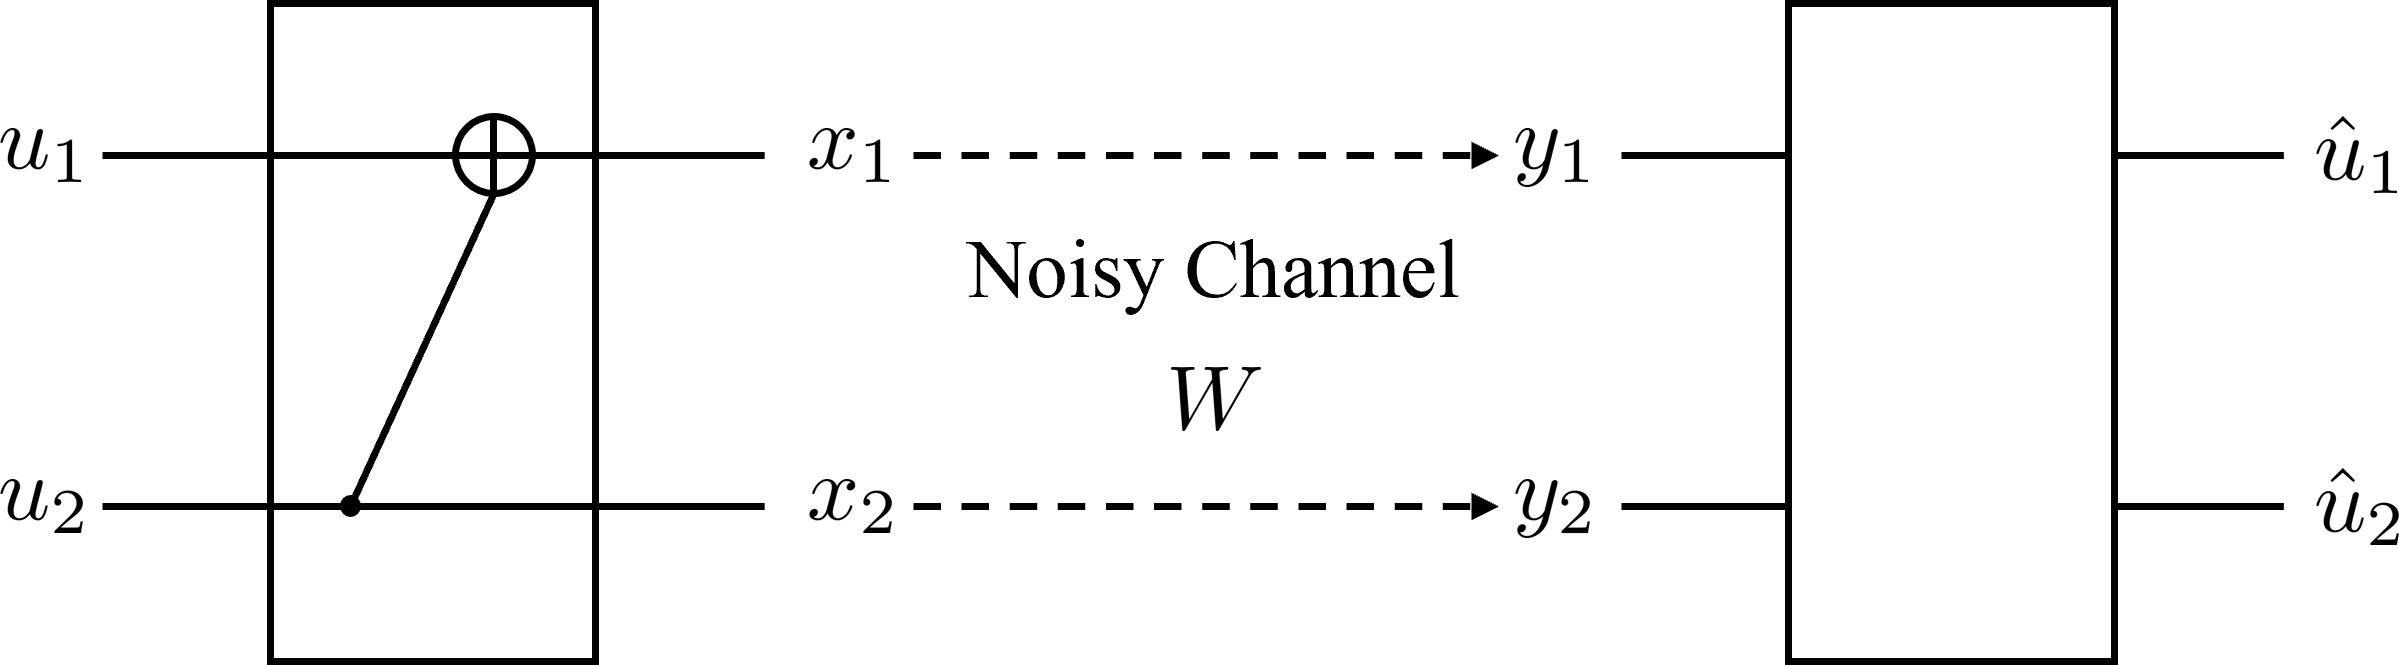
\includegraphics[width=0.7\linewidth]{w1_channel.png}
    \caption{Single-layer polar code.}
    % \label{fig:enter-label}
\end{figure}
We have $y_1$ and $y_2$ being the channel outputs to the channel inputs $x_1=u_1\oplus u_2$ and $x_2=u_2$, respectively, where $\oplus$ is the addition modular 2. If the context is clear, we may write $\oplus$ simply as $+$. If the channel $W$ is faithful, then we can simply set the estimates as $\hat{u}_1 = y_1 \oplus y_2$ and $\hat{u}_2 = y_2$. However, since our channel is noisy, this is simply not the case. What Ar{\i}kan did to construct $\hat{u}_1$ and $\hat{u}_2$ from $y_1$ and $y_2$ was the following procedure:
\begin{enumerate}
    \item Guess $u_1$ by looking at $y_1$ and $y_2$, either via sufficient statistics, or by consensus.
    \item Assume that we did get $u_1$ right, guess $u_2$ by looking at $y_1$, $y_2$, and $u_1$.
\end{enumerate}

What was Ar{\i}kan's motivation for considering the above channel coding scheme? How did he came up with the ``magical'' decoding procedure? First off, one needs to know that his considering of this transformed channel is motivated by the improving of the \textit{cutoff rate} of a channel.

\newpage %formatting

\begin{definition}[Cutoff Rate]
    Given a channel $W:x\rightarrow y$, the cutoff rate is defined as
    \begin{equation}\begin{aligned}
        R_0(W) \defeq&~ \max_{Q\in\Delta(\mathcal{X})}-\lg \sum_{y\in\mathcal{Y}}\left(\sum_{x\in\mathcal{X}}Q(x)\sqrt{W(y\vert x)}\right)^2 \\
        =&~\text{ the rate at which we can communicate ``easily.''}
    \end{aligned}\end{equation}
\end{definition}
Though the mathematical definition of the cutoff rate is fairly complicated, let us only focus on the text description of its purpose: one can immediately tell that $0 < R_0(W) \le C(W)$, where $C(W)=\max_{P_X}I(X;Y)$ is the channel capacity, the theoretical maximum rate for communication over a noisy channel.

Let us denote the whole channel from the bits to the estimates as
\begin{equation}\begin{aligned}
    W^{-} &: u_1 \rightarrow \hat{u}_1, \\
    W^{+} &: u_2 \rightarrow \hat{u}_2.
\end{aligned}\end{equation}
Ar{\i}kan made the following critical observation on the two sub-channels above.

\textbf{Observation}: The cutoff rate of the channel increases:
\begin{equation}
    R_0(W^{-}) + R_0(W^{+}) \ge 2\cdot R_0(W), \label{eq:w1_cutoff_rate_ineq}
\end{equation}
where the inequality is almost always strict.

\begin{remark}
    Note that the capacity remains unchanged:
    \begin{equation}
        C(W^{-}) + C(W^{+}) = 2\cdot C(W).
    \end{equation}
    The equality sign to the cutoff rate inequality \autoref{eq:w1_cutoff_rate_ineq} holds when $W$ is ``extreme'', what is its definition?
\end{remark}

If there is a trick that can increase the cutoff rate \textit{costlessly}, we can do it again and again: an example will be to do it twice, see the figure below.
\begin{figure}[H]
    \centering
    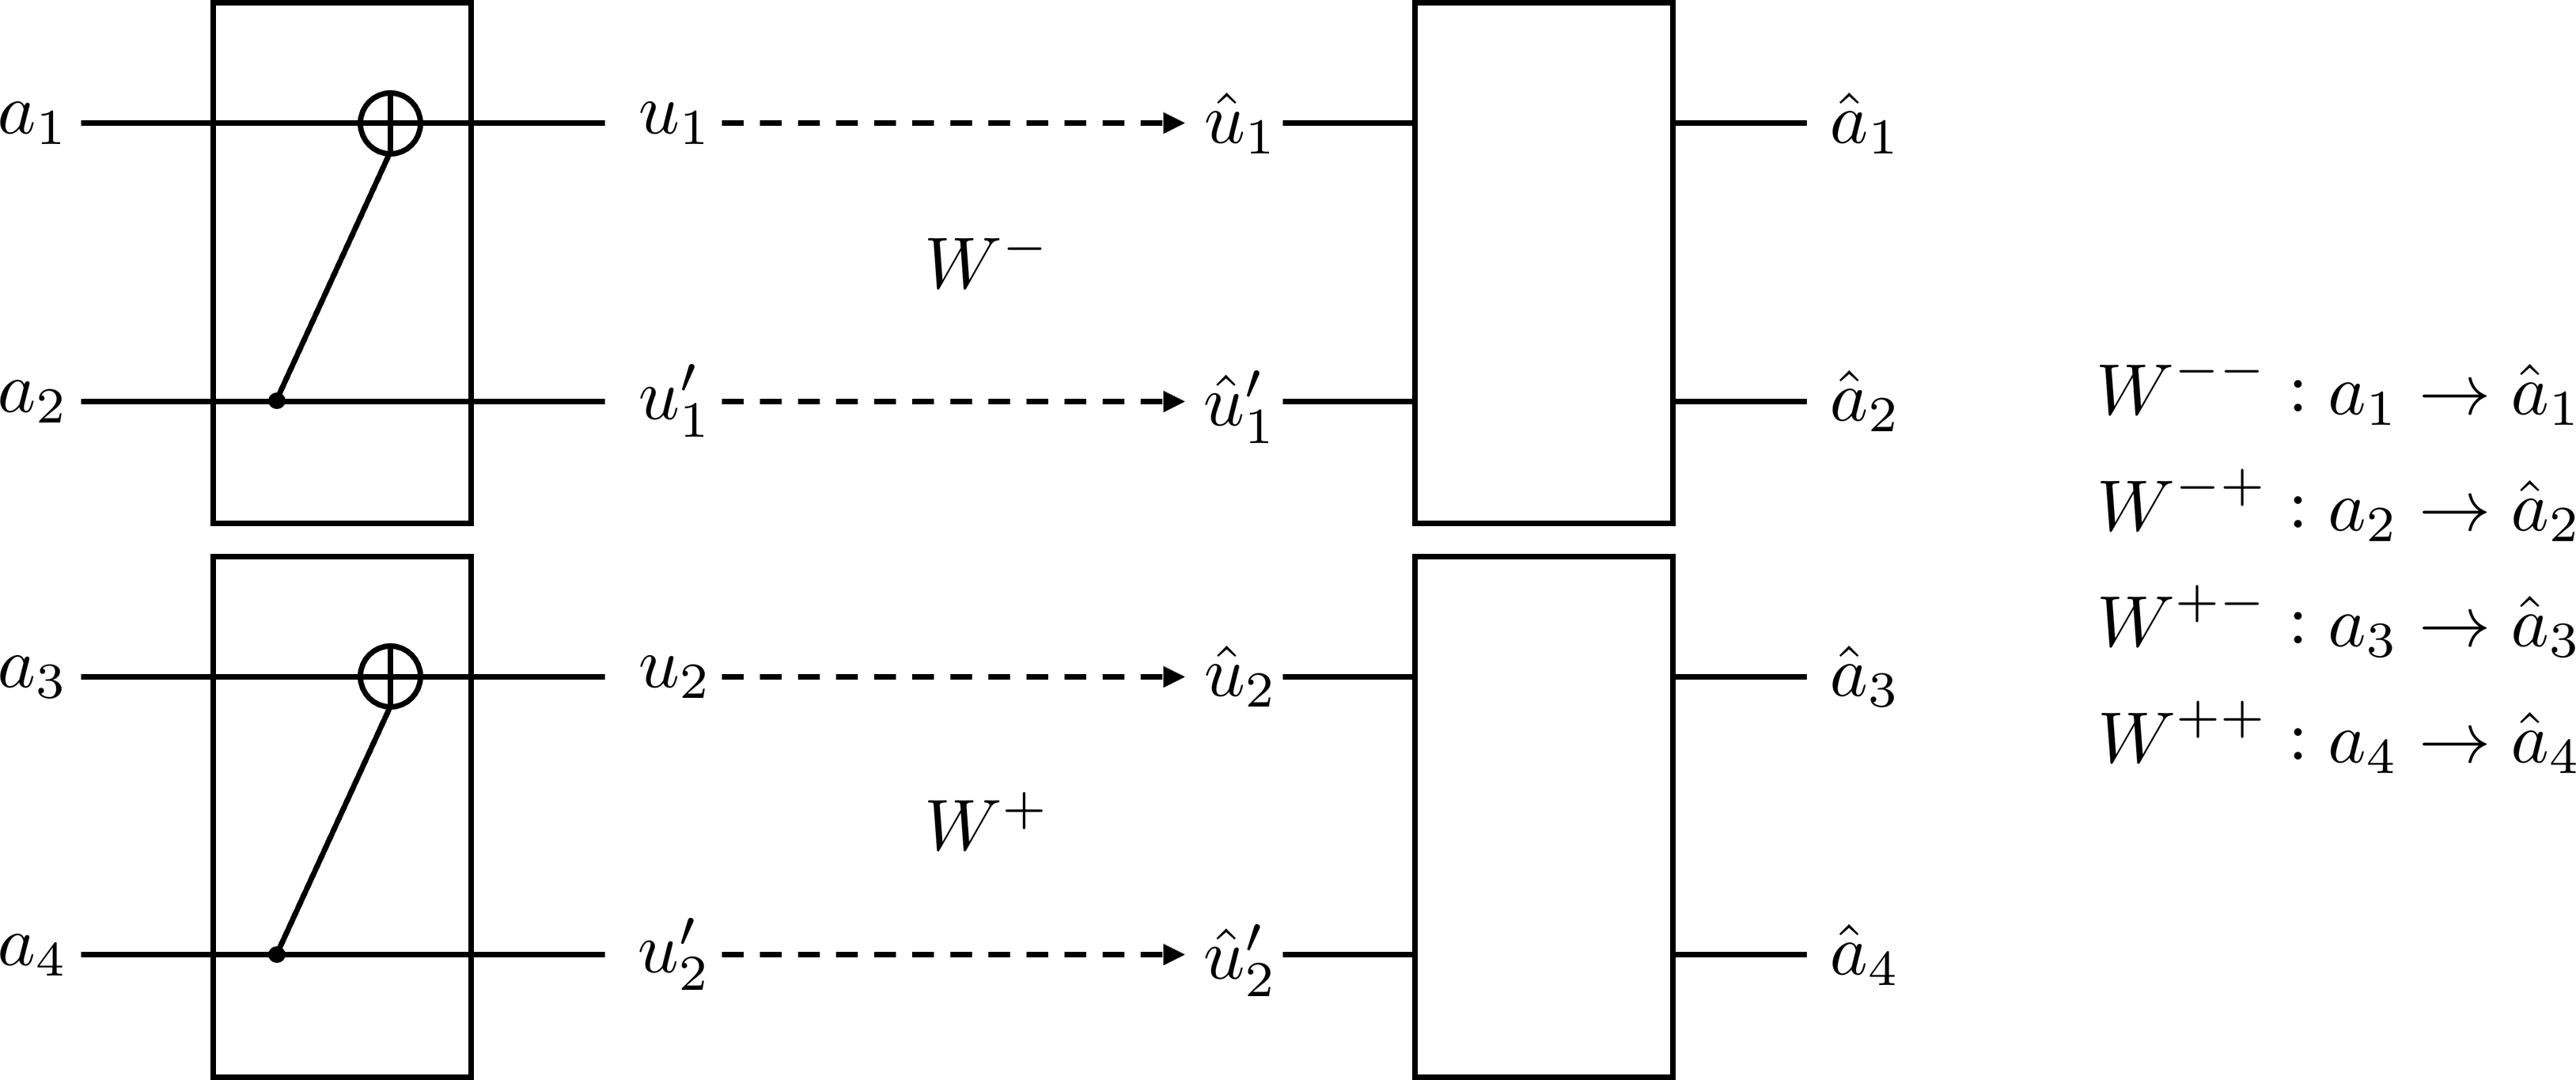
\includegraphics[width=0.8\linewidth]{w1_split_channel.png}
    \caption{Splitting channels.}
    % \label{fig:enter-label}
\end{figure}

Now we have four new sub-channels indexed by the string $s\in\{+,-\}^2$, denoting whether they are from the $+$ or the $-$ branch. The average cutoff rate thus increases further:
\begin{equation}
    R_0(W^{--}) + R_0(W^{-+}) + R_0(W^{+-}) + R_0(W^{++}) \ge 2\cdot R_0(W^{-}) + 2\cdot R_0(W^{+}) \ge 4\cdot R_0(W).
\end{equation}

\textbf{Observation}: if we repeat it indefinitely, then the average cutoff rate will continue to increase with an upper bound of $C(W)$. This bound \textit{can}, in fact, be reached:
\begin{equation}
    \frac{1}{2^n} \sum_{s\in\{+,-\}^n} R_0(W^s) \xrightarrow{n\rightarrow\infty} C(W) = \frac{1}{2^n}\sum_{s\in\{+,-\}^n} C(W^s).
\end{equation}

Amazingly, we seem to have to accept that coding at any rate under the channel capacity is ``easy.''  At this stage, Ar{\i}kan have almost invented polar code.

\section{Why ``Polar''? Asymptotic Behaviors of Polar Codes}

This section is from the paper ``Channel polarization: A method for constructing capacity-achieving codes for symmetric binary-input memoryless channels'' \cite{Channel_Polarization}. The usage of the word ``polar'' comes from the following observation:

\textbf{Observation}: For most strings $s\in\{+,-\}^n$, the values $C(W^s)$ and $R_0(W^s)$ are ``almost'' close to 0 or 1. So that the sub-channels are ``polarized.''

To wrap up, let us combine our observations above:
\begin{enumerate}
    \item $\frac{1}{2^n}\sum_{s\in\{+,-\}^n}C(W^s) = C(W)$.
    \item $C(W^s)$ is either very close to 0 or 1.
    \item The number of strings $s$ such that $C(W^s)=1$ is about $2^n C(W)$; the number of strings $s$ such that $C(W^s)=0$ is about $2^n \left(1 - C(W)\right)$.
\end{enumerate}
As a first example, let us see the easiest case of polar code over binary erasure channels. The cases for BSC, AWGN, or other general channels are harder and is considered later.

Observe that fixing an $s$ such that $C(W^s) \approx 1$, $W^s$ is such a good channel that we can transmit messages ``\textit{uncoded},'' and most of the time it transmits messages faithfully. Funnily enough, we can forget cutoff rate as a whole. We will send uncoded messages over the good sub-channels $W^s$ where $C(W^s) \approx 1$, and send deterministic bit values of 0 over the bad ones, we have the code rate as
\begin{equation}
    \text{Code rate} = \frac{\text{\# bits transmitted}}{\text{\# channel uses}=2^n} \approx C(W).
\end{equation}
Hence, polar code is capacity-achieving. All that is left is to focus on what the ``magic decoding procedures'' are from $y_i$'s to $\hat{u}_i$'s.

\begin{remark}\label{rmk:1.2}
    For $n=1$, we denote $W^{+}$ as the good sub-channel and $W^{-}$ as the bad sub-channel. Agreeing on sending 0's across the bad sub-channels ensures that we know that $\hat{u}_1$ is, and hence is good for obtaining the estimate $\hat{u}_2$ over $W^{+}$.
\end{remark}


\subsection{Binary Erasure Channel}
A binary erasure channel is a tuple represented by $(\mathcal{X},\mathcal{Y},W)$, where $\mathcal{X} = \{0,1\}$ is the input alphabet, $\mathcal{Y} = \{0,1,\mathcal{E}\}$ is the output alphabet, $\mathcal{E}$ is the erasure symbol, and
\begin{equation}
    W = \left[\begin{matrix}
        1-p & 0 & p \\
        0 & 1-p & 0
    \end{matrix}\right]
\end{equation}
is the transition matrix (see diagram below). One should be careful that in literature, the misleading notational similarity between the transition probability $W(y\vert x)$ and posterior probability $W(x|y)$ exists, one should be careful of which one is used.
\begin{figure}[H]
    \centering
    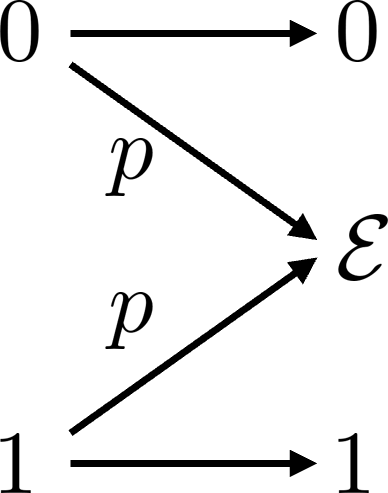
\includegraphics[width=0.1\linewidth]{w1_erasure.png}
    \caption{Illustration of a binary erasure channel.}
    % \label{fig:enter-label}
\end{figure}

A BEC is parameterized by its erasure probability $p\in[0,1]$, i.e., a BEC channel can be simply denoted uniquely as $\mathrm{BEC}(p)$.

Why do we want to use the BEC as a first example? It is due to the following two properties:
\begin{lemma}[Properties of BEC]
    \begin{enumerate}
        \item The sub-channels $\mathrm{BEC}^{+}$ and $\mathrm{BEC}^{-}$ are still BECs!
        \item We have 
        \begin{align}
            \mathrm{BEC}^{+}(x) &= \mathrm{BEC}(x^2), \label{eq:w1_bec+}\\
            \mathrm{BEC}^{-}(x) &= \mathrm{BEC}(2x-x^2). \label{eq:w1_bec-}
        \end{align}
    \end{enumerate}
\end{lemma}

\begin{lemma}[Channel Capacity of BEC]
    \begin{equation}
        C\left(\mathrm{BEC}(x)\right) = 1-x
    \end{equation}
\end{lemma}

\begin{proof}
    Let $X\sim \mathrm{Ber}(\alpha)$, then the mutual information will be
    \begin{align*}
        I(X;Y) &= H(Y) - H(Y|X) \\
        % &= -\left[\alpha(1-p) \lg\alpha(1-p) + (1-\alpha)(1-p) \lg(1-\alpha)(1-p) + p \lg p\right] \\
        % &\;\;\;\;\;+ \left[\alpha \cdot \left(p\lg p + (1-p)\lg(1-p)\right) + (1-\alpha) \cdot \left(p\lg p + (1-p)\lg(1-p)\right)\right] \\
        &= -\alpha(1-p) \lg\alpha(1-p) - (1-\alpha)(1-p) \lg(1-\alpha)(1-p) + (1-p)\lg(1-p).
    \end{align*}
    The maximum is achieved at
    \begin{align*}
        \diff{}{\alpha} I(X;Y) = 0 &= -(1-p)\left(\lg\alpha(1-p) + 1\right) + (1-p)\left(\lg(1-\alpha)(1-p) + 1\right) \\
        &\rightarrow \lg\alpha = \lg(1-\alpha) \rightarrow \alpha = \frac{1}{2}.
    \end{align*}
    Hence the channel capacity is
    \begin{align*}
        C\left(\mathrm{BEC}(p)\right) = \left.I(X;Y)\right|_{\alpha=\frac{1}{2}} = -(1-p)\lg\frac{1-p}{2} + (1-p) \lg (1-p) = (1-p).
    \end{align*}
    Thus it is proven.
\end{proof}

From the above lemmas, we can check that BEC satisfies our previous observation:
\begin{equation*}
    C\left(\mathrm{BEC}(p)^{+}\right) + C\left(\mathrm{BEC}(p)^{-}\right) = (1-x^2) + (1-2x+x^2) = 2-2x = 2\cdot C\left(\mathrm{BEC}(p)\right).
\end{equation*}
Further, for the $+$ channels, the erasure probability reduces to $x^2$, while for the $-$ channels, the erasure probability increases to $1-(1-x)^2$. The $+$ channels quickly become faithful as their erasure probability $p\rightarrow 0$, while the $-$ channels quickly become useless as $p\rightarrow1$. A quantitative description is as follows:
\begin{theorem}[Speed of Polarization] \label{thm:w1_polar_speed}
    There exists a function $f:[0,1] \rightarrow [0,1]$ that has shape quite similar to $[x(1-x)]^{0.7}$ satisfying the following functional equation:
    \begin{equation}\label{eq:w1_speed_of_polarization_1}
        \frac{f(x^2) + f(2x-x^2)}{2f(x)} \approx 2^{-\frac{1}{3.627}} \approx 0.826.
    \end{equation}
    Consequently,
    \begin{equation}\label{eq:w1_speed_of_polarization_2}
        \frac{1}{2^nf(x)} \sum_{s\in\{+,-\}^n} f\left(\text{erasure probability of }\mathrm{BEC}(x)^s\right) \approx 2^{-\frac{n}{3.627}} \approx 0.826^n.
    \end{equation}
\end{theorem}
Since the RHS of the above equation is small, most of ``$f\left(\text{erasure probability of }\mathrm{BEC}(x)^s\right)$'' is small as well. Looking at the graph of $f\approx[x(1-x)]^{0.7}$, we see that $x$ must be close to 0 or 1. Henceforth, $\mathrm{BEC}^s(x)$ is mostly equal to either $\mathrm{BEC}(0)$ or $\mathrm{BEC}(1)$. What's more, the theorem above states that the quantitative speed of channel polarization is exponential in the order of $2^{-\frac{n}{3.627}}$. For general channels, we have the speed of polarization in the order of $2^{-\frac{n}{4}}$, with a mathematically rigorous bound currently at $2^{-\frac{n}{4.71\cdots}}$. Moreover, the derivation from \autoref{eq:w1_speed_of_polarization_1} to \autoref{eq:w1_speed_of_polarization_2} is as follows:
\begin{proof}
    Assume such $f$ exists, then plugging in $x^2$ and $2x-x^2$, we obtain
    \begin{equation*}
    \begin{cases}
        f(x^4) + f(2x^2-x^4) = 2^{-\frac{1}{3.627}}\cdot 2 f(x^2) \\
        f((2x-x^2)^2) + f(2(2x-x^2)-(2x-x^2)^2) = 2^{-\frac{1}{3.627}}\cdot 2 f(2x-x^2)
    \end{cases}.
    \end{equation*}
    Then, we have
    \begin{align*}
        f(x^4) + f(2x^2-x^4) &+ f((2x-x^2)^2) + f(2(2x-x^2)-(2x-x^2)^2) \\
        &= 2^{-\frac{1}{3.627}}\cdot2\left(f(x^2) + f(2x-x^2)\right) = 2^{-\frac{2}{3.627}}\cdot 4f(x).
    \end{align*}
    Continue on this trend, we will obtain \autoref{eq:w1_speed_of_polarization_2} by induction.
\end{proof}
\autoref{eq:w1_speed_of_polarization_1} is sort of like an eigenvalue problem, with $f$ as the eigenfunction and $2^{-\frac{1}{3.627}}$ as the eigenvalue. As of when this script was written, the only method for proving and showing speed of polarization is using the above ``power-sum method'' or some other similar variants. For more details, also refer to the paper ``On the rate of channel polarization'' \cite{On_the_Rate_of_Channel_Polarization}.

If the erasure probability $x$ is very small, say $2^{-20}$, then $x^2 = 2^{-40}$ and $2x - x^2 \approx 2^{-19}$. We can approximate the sub-channels as
\begin{equation}
    \mathrm{BEC}(x)^s \approx \mathrm{BEC}(x^{\overbrace{2\times\cdots\times 2}^{\text{\# of $+$'s in $s$}}}).
\end{equation}

Then, for arbitrary $s\in\{+,-\}^n$, as a conservative bound we have about $n(\frac{1}{2}-\varepsilon)$ of $+$'s in $s$ with high probability. Then if $x$ is small, then most $\mathrm{BEC}(x)^s \approx \mathrm{BEC}(x^{2^{n/2}})$. Further recall that the amount of strings $s$ such that $\mathrm{BEC}(x)^s$ has small erasure probability is $2^n C\left(\mathrm{BEC}(x)\right)$. Now we know that not only are a fraction (approximately $C(W)$) of $W^s$'s are good, but they are also approximately $\mathrm{BEC}(x^{2^{n/2}})$-good, i.e., we have good channels that are ``exponentially exponentially decaying!''

% \section{Agenda}
The agenda for this course will hence be to prove the \textit{observations} and facts listed above. Further, we will also discuss generalizations of polar codes: BEC, BSC, AWGN, asymmetric channels, deletion channels, Markovian channels, non-stationary channels, source coding, rate distortion, wiretap, broadcast, multiple access channels, larger alphabet, larger kernel, $\ldots$.


\section{The Big Picture}
There is a correspondence between probability theory and coding theory:

\begin{table}[H]
    \centering
    \begin{tabularx}{\textwidth}{X|X|X}
        \multicolumn{1}{c}{Probability Theory} & \multicolumn{1}{c}{Random Codes} & \multicolumn{1}{c}{Polar Codes} \\ \hline\hline
        For i.i.d. $X_1,\ldots,X_N$, we have the \textit{concentration inequality}:
        \resizebox{\linewidth}{!}{
        $\begin{aligned}
            \mathrm{Pr}\left\{\frac{X_1+\cdots+X_N}{N} -\mathbb{E}[X_1] \ge t\right\} \\ \le \exp(-ct^2N)
        \end{aligned}$
        }
        for some constant $c$. This is also known as the \textit{large deviation principle / behavior}, it can be derived from Hoeffding's inequality. &
        Over a channel $W$ with fix rate $R<C(W)=C$, let the block length be $N$. Then there exists a good code of block error probability
        \begin{equation*}
            \approx \exp(-c(C-R)^2N)
        \end{equation*}
        for some constant $C$. &
        At block length $N$, code rate $R<C$, the bound for error probability is $\approx\exp(-\sqrt{N})$ for polar code, and can be improved to $\approx\exp(-N^{0.9})$ for other schemes.\\ \hline
        The central limit theorem (CLT) states that
        \resizebox{\linewidth}{!}{
        $\begin{aligned}
            Z \defeq \frac{X_1+\cdots+X_N}{\sqrt{N}} - \sqrt{N}\mu \\ \sim \mathcal{N}(0,\sigma^2),
        \end{aligned}$
        }
        where $\mu=\mathbb{E}[X_1]$ and $\sigma^2=\mathrm{Var}(X_1)$. This is also known as the \textit{small deviation principle}. & 
        At block length $N$, and fix $p$ as block error probability. The code rate is
        \begin{equation*}
            R \approx C- O\left(\frac{1}{\sqrt{N}}\right).
        \end{equation*} &
        At block length $N$, and fix $p$ as block error probability. The code rate is
        \begin{equation*}
            R\approx C-O(N^{-1/3.6})
        \end{equation*}
        for polar code, and the exponent can be improved to $N^{-1/2.1}$. \\ \hline
        The \textit{moderate deviation principle} asks what is the distribution that the following R.V. follows?
        \begin{equation*}
            Y \defeq \frac{X_1+\cdots+X_N}{N^\alpha}-\frac{N\mu}{N^\alpha}
        \end{equation*} &
        There is a tradeoff between $R$ and $p$. &
        There is a tradeoff between $R$ and $p$.
    \end{tabularx}
    % \caption{Caption}
    % \label{tab:my_label}
\end{table}
As a side note, if the polar code is $n$-layer deep, then the block length $N=2^n$.

This big picture is what one should keep in mind throughout this lecture note. Further note that the results for coding theory are often proved using random coding, which is not really practical. Hence, we also provided the bounds for practical codes such as the polar codes in the table above.

% \begin{remark}[Block Length]
%     In case one forgot, the block length $N$ of a code is the number of bits in a block. It is related to the number $n$ defined in \autoref{sec:w1_origin_of_polar_code} by $N=2^n$.
% \end{remark}

% The relation between small, moderate, and large deviation behaviors are also seen in source coding and hypothesis testing. See the lecture slides by prof. Hao-Chung Cheng on Quantum Compression, Classical Communication in the course Quantium Information and Computation for nice illustrations and more information. An excerpt from the source coding theory is shown in the figure below:
% \begin{figure}[H]
%     \centering
%     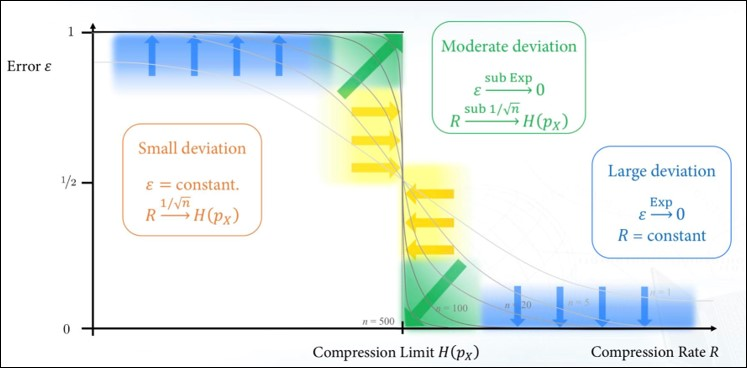
\includegraphics[width=0.8\linewidth]{figures/w1_deviation.jpg}
% \end{figure}


\chapter{Polar Codes}
\lecture{25 Feb.}

At the end of the last chapter, we characterize the behavior of codes in the asymptotic regime due to the fact that they are easier to compute and analyze. This chapter starts off by developing the essential tools in obtaining these concentration inequalities. Further, the Shannon's channel coding theorem on noisy channels is also introduced as an inspiration on how information is possible to be transmitted through erroneous channels.

Next, we delve into the theory and analysis of polar codes over noisy channels. Using tools such as the martingale theory, we see how the many observations mentioned from the last chapter are actually derived.

\section{Concentration Inequalities}
Given a collection of random variables, say $X_1$, $X_2$, $\ldots$, and $X_n$, that may or may not be independent or identically distributed, we would like to \textit{control} their joint distribution. A way to control their joint distribution is to bound their moments, an example would be to assume that they are independent and identically distributed (i.i.d.), then we know that
\begin{equation*}
    \frac{X_1+\cdots+X_n}{n} \approx \mathbb{E}[X_1].
\end{equation*}
The following theorem will be to characterize in what way does ``$\approx$'' hold.

\begin{theorem}[Hoeffding's Inequality]
    For i.i.d. R.V.s $X_1$, $\ldots$, and $X_n$, there exists a real number $c>0$ dependent on the distribution such that
    \begin{equation}
        \mathrm{Pr}\left\{\frac{X_1+\cdots+X_n}{n} - \mathbb{E}[X_1] \ge t\right\} \le \exp\left(-cnt^2\right).
    \end{equation}
\end{theorem}
The exact value to $c$ doesn't matter, and may vary from text to text. All that one has to know is that as long as $n\rightarrow\infty$, the bound approaches zero exponentially.

Let us consider a simple example on Bernoulli random variables and see that the Hoeffding's inequality indeed holds.
\begin{example}
    Consider i.i.d. $X_1$, $\ldots$, $X_n\sim\mathrm{Ber}(0.5)$ and $t>0$, we have
    \begin{align*}
        \mathrm{Pr}\left\{\frac{X_1+\cdots+X_n}{n} - \frac{1}{2} \ge t\right\} &= \mathrm{Pr}\left\{X_1+\cdots+X_n \ge n\left(t+1/2\right)\right\} \\
        &= \mathrm{Pr}\left\{\exp\left(s(X_1+\cdots+X_n)\right) \ge \exp\left(s\left(nt+n/2\right)\right)\right\}.
    \end{align*}
    This holds for all $s<0$, hence
    \begin{align*}
         \mathrm{Pr}\left\{\frac{X_1+\cdots+X_n}{n} - \frac{1}{2} \ge t\right\} &\le \inf_{s>0} \frac{\mathbb{E}\left[\exp\left(s(X_1+\cdots+X_n)\right)\right]}{\exp\left(s(nt+n/2)\right)} \\
        &= \inf_{s>0} \frac{\left[\frac{1}{2}(1+\ee^s)\right]^n}{\exp\left(s(nt+n/2)\right)}\;\;\;\;\;(\text{consider the MGF}) \\
        &\eqdef \exp(-cn),
    \end{align*}
    where
    \begin{equation*}
        c = \frac{1}{2}(2t+1)\ln\left(\frac{1+2t}{1-2t}\right) + \ln\left(1-2t\right) \gtrsim 2t^2 > 0.
    \end{equation*}
    Thus, it is shown. The right hand side to the first inequality written above is known as the Chernoff bound.
\end{example}


\begin{remark}
    There are two ways to generalize the Hoeffding's inequality:
    \begin{enumerate}
        \item find the best $c$.
        \item use non-i.i.d. random variables.
    \end{enumerate}
    
    Amazingly, if the random variables ${X_i}'s$ are correlated, or even not identically distributed, we can still obtain similar results! But the details are more technical.

    Consider the example on Bernoulli R.V.s above, replacements are required in calculating the expectation $\mathbb{E}\left[\exp(s(X_1+\cdots+X_n))\right]$. We need a different way to bound this expectation.

    This introduces us to the theory of \textit{sub-Gaussian random variables}. A random variable is called sub-Gaussian if $\mathbb{E}[\ee^{tX}] < \ee^{ct^2}$ for some constant $c$. This definition is motivated by the bounding of the tail probability: for $t>0$,
    \begin{equation}
        \mathrm{Pr}\{X\ge t\} = \mathrm{Pr}\left\{\exp(sX)\ge\exp(st)\right\}  \le \mathbb{E}[\exp(sX)] \ee^{-st} = \ee^{cs^2-st} \stackrel{s=\frac{t}{2c}}{=} \ee^{-\frac{t^2}{4c}}.
    \end{equation}
    All bounded random variables are sub-Gaussian. For a weaker decaying tail, one may use the \textit{sub-gamma random variables} to bound the tail probability.

    Another nice property of sub-Gaussians is that their sum concentrates the mean, hence we have that their average having a smaller and smaller variance. The same thing sadly does not apply for sub-Gammas.
\end{remark}

Besides the Chernoff bound and Hoeffding's inequality, the Chebyshev inequality and Markov inequality are also commonly used bounds. It is interesting to note that Chebyshev is actually the teacher of Markov and some may regard all the inequalities above as just special cases of Markov's inequality.




\section{Shannon's Noisy-Channel Coding Theorem}
A very well written paper which forms the onset of the information theory is C. E. Shannon's 1948 paper ``A Mathematical Theory of Communication'' \cite{Shannon}, in which the famous results such as source-channel separation, source coding, and channel coding are given.

\subsection{Channels}
In the first chapter, we have introduced terms such as capacity and rate, which are properties of a channel. So what exactly are channels? We shall illustrate them with examples.

The first three discrete channels shown below are, in order from left to right, \textit{binary erasure channel} (\textit{BEC}), \textit{binary symmetric channel} (\textit{BSC}), and Z-channel. The probability $p$ in BEC is termed the erasure probability; the probability $p$ in BSC is termed the cross-over probability.
\begin{figure}[H]
    \centering
    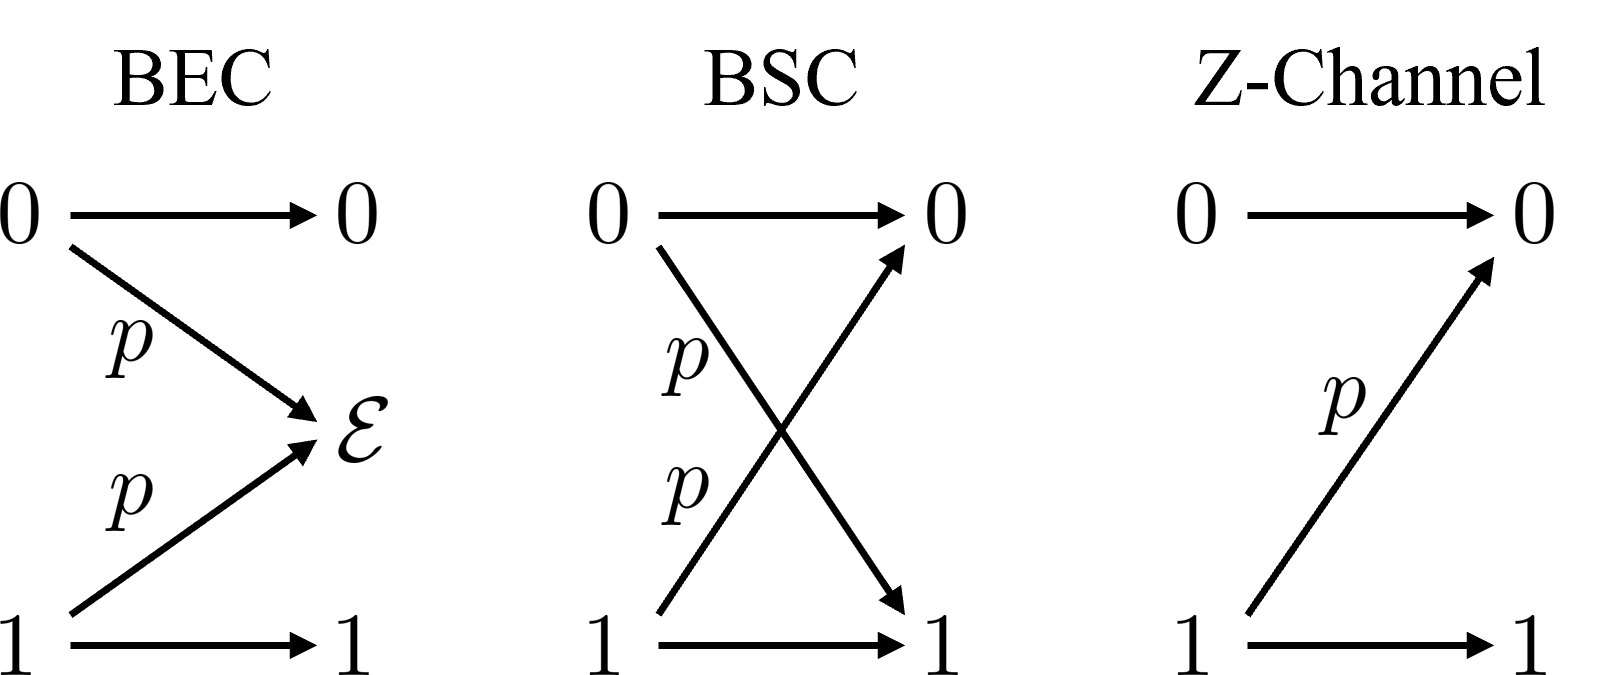
\includegraphics[width=0.5\linewidth]{figures/w2_discrete_channels.png}
    \caption{Some common channels: binary erasure channel, binary symmetric channel, Z channel.}
\end{figure}
Note that the Z-channel is a really bad channel. Though it seems to be a much simpler channel in comparison to BEC or BSC, it is bad since we cannot use linear code on it. The literature on linear code is so vast and widely used that if a channel cannot use linear code, the channel is deemed as a bad one.

Another example of a channel would be the continuous \textit{additive white Gaussian noise} (AWGN) channel. See the figure below, when an input bit is sent, a white (unbiased) Gaussian noise of variance $\sigma^2$ is added, resulting in a continuous spectrum of possible received signal.

\begin{figure}[H]
    \centering
    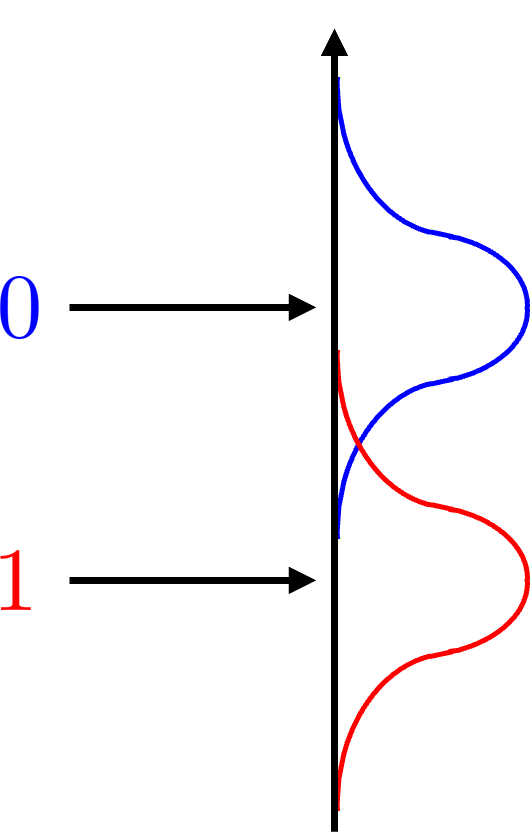
\includegraphics[width=0.15\linewidth]{figures/w2_AWGN.png}
    \caption{Additive white Gaussian noise channel.}
\end{figure}

In general, a discrete memoryless channel is characterized by the tuple $(\mathcal{X},\mathcal{Y},W)$, where the transition probability from $x\in\mathcal{X}$ to $y\in\mathcal{Y}$ is $W(y\vert x)$.

\subsection{Shannon's Noisy-Channel Coding Theorem}
Here we give a more hand-wavy description of Shannon's theory, relating the capacity, rate, allowed error of a channel with its possibility to transmit information.

\begin{theorem}[Noisy-Channel Coding Theorem]
    For a channel $W$, there exists a number $C(W)>0$, such that one can transmit $C(W)-\varepsilon$ bits per usage and guarantee the existence of a code with error probability arbitrarily small.
\end{theorem}

First off, this is a highly \textit{non-trivial} result! How is it even possible for one to transmit information in the face of noises and errors? 

Let us consider the following demonstration using BEC: select a subset $\mathcal{C}\subset\{0,1\}^n$ of \textit{codewords} for transmission. For example, in the case of $n=3$, the repetition code is $\mathcal{C}=\{000,111\}$, sending 000 if the message 0 is to be sent, sending 111 if the message 1 is to be sent. The repetition code has a code rate of $R=(\#\text{ of bits of information sent})/(\#\text{ of channel use}) = 1/3$. Can we do better? Yes, consider sending the message 1, 2, 3, and 4 with the codewords $\mathcal{C}=\{000,011,101,110\}$. This code has a code rate of $R=2/3$. And in the face of erasure, we can still determine the message most of the time: the decoder will be
\begin{align*}
    \mathrm{Dec}: 1\mathcal{E}0 &\mapsto 110 = \text{message 4} \\
    00\mathcal{E} &\mapsto 000 = \text{message 1} \\
    1\mathcal{EE} &\mapsto ?
\end{align*}
Notice that if two or more erasures occur, the above code will not have perfect reconstruction. But this is alright, since we can just try again and again to decrease the failure probability.

A characteristic of the above demonstration is that when we increase the code rate, the error probability also increases. In practical designs, we care more about the increasing code rate instead of reducing the error probability, after all, who knows the difference between $10^{-6}$ and $10^{-9}$?

Here we will give a more detailed example regarding the existence of a good coding scheme on BEC.
\begin{example}
    Consider transmission with the channel $\mathrm{BEC}(0.5)$. Suppose that $n$ is big, and we can pick a $\mathcal{C}\subset\{0,1\}^n$. How do we choose good codewords $\mathcal{C}$? A common strategy for theoretical analysis is by \textit{random coding}.

    First, let us consider picking random codewords $w^1$ and $w^2\in\{0,1\}^n$. Let us send $w^1$ over $W$ to obtain, for example
    \begin{equation*}
        W:w^1 = 0011011\ldots \mapsto 0\mathcal{E}110\mathcal{E}1\ldots=y,
    \end{equation*}
    a question will be to ask what is the error probability that $y$ is \textit{compatible} with $w^2$?

    The received $y$ will be compatible with $w^2$ if for all index $1$ to $n$, either $y_i=\mathcal{E}$, or that $w^2_i=y_i=w^1_i$, each happening with probability $\frac{1}{2}$ and $\frac{1}{2}\cdot\frac{1}{2}=\frac{1}{4}$. So the total probability of a single bit being compatible will be $\frac{3}{4}$. So as $n\rightarrow \infty$, $y$ is compatible with $w^2$ with a probability of $\left(\frac{3}{4}\right)^n\rightarrow0$, meaning the two are incompatible. Moreover, we know that $y$ is compatible with $w^1$ with a probability of $1-\left(\frac{3}{4}\right)^n\rightarrow1$, meaning we have a high probability of knowing $y$ is indeed $w^1$.

    
\end{example}
However good the success probability may be, the rate of the above scheme is $R=1/n\rightarrow 0$. Can we do any better?
\begin{example}
    Consider the same as above, but this time, we allow for a larger set of codewords: $\mathcal{C}=\{w^i\}_{i=1}^m$. By including $m$ codewords, we can ask the same question on the compatibility of $y$ with $w^2$, $w^3$, $\ldots$, and $w^m$, and obtain a \textit{lower} bound on the success probability being
    \begin{equation*}
        \mathrm{Pr}\{\text{success detecting $w^1$ from $y$}\} = 1-(m-1)\left(\frac{3}{4}\right)^n.
    \end{equation*}
    And by choosing $m\approx\frac{1}{100}\left(\frac{3}{4}\right)^n$, we have the success probability being approximately $99\%$ with a non-zero code rate of
    \begin{equation*}
        R = \frac{\# \text{ bits of information sent}}{\# \text{ channel use}} = \frac{\lg m}{n} = \frac{\lg\left(\frac{3}{4}\right)^n}{n} = 0.415,
    \end{equation*}
    where $\lg(\cdot)=\log_2(\cdot)$. This is a constant code rate scheme!
\end{example}
Note that for the $\mathrm{BEC}(0.5)$ channel, the theoretical limit is $R=0.5$, which is the capacity of the channel. We can certainly improve further, but what is the problem with our analysis above that made it not able to saturate the bound? The devils are in the details. The ``bad events'' have intersections, and the over-estimation of the error probability costs us some capacity. For example, the all erasure string $\mathcal{EE\ldots E}$ is compatible with all ${w^i}'s$. A more careful analysis should be able to achieve the bound.

\begin{remark}
    The above analysis utilizes random codes. But it is only good for theory, since the implementation of its encoder and decoder requires $\exp(\mathrm{O}(n))$ of calculations. In practice, we need \textit{low complexity codes}. As we will see later, polar codes has the complexity of $\mathrm{O}(n\lg n)$.
\end{remark}

As an end to this chapter on the noisy-channel theorem, let us also consider another example on BSC. What happens with BSC and random coding? Just on an intuitive level, one should be able to obserbe the following:
\begin{enumerate}
    \item The channel $\mathrm{BSC}(0.5)$ is a bad channel (though it is a really good random seed generator).
    \item Our analysis should use $\mathrm{BSC}\left(1/4\right)$ instead.
    \item The channel $\mathrm{BSC}\left(3/4\right) = \mathrm{BSC}\left(1/4\right)$ since one can simply flip the 0 and 1 after passing through the former to obtain the latter.
    \item Pick $w^i\in\{0,1\}^n$ randomly, send $w^1=00\ldots0$.
    \item Obtain $y$, compute compatibility with $w^1$ by \textit{Hamming distance}. One should obtain $d_\mathrm{H}(y,w^1)\approx \frac{n}{4}$.
    \item Compute the compatibility of $y$ with other codewords, for example, $d_\mathrm{H}(y,w^2) \approx \frac{n}{2}$.
    \item We can set the decoding algorithm to be: If $d_\mathrm{H}(y,w^i)<\frac{n}{3}$, then we determine it to be $w^i$.
    \item The above decoding scheme fails when: (w.p. = with probability)
    \begin{enumerate}[label=(\arabic*)]
        \item $d_\mathrm{H}(y,w^1) > \frac{n}{3}$, w.p. $\le\left(\frac{1}{4}\right)^{n/3}$ (define this error to be $\alpha$), or
        \item $d_\mathrm{H}(y,w^{i\neq1}) < \frac{n}{3}$, w.p. $\le \left(\frac{1}{2}\right)^{2n/3}$ (define this error to be $\beta$).
    \end{enumerate}
    \item We can further bound the above via Chernoff bound: for $i=1\sim n$, let $F_i=1$ if the $i$th bit of $w^1$ is flipped to obtain $y$, else it is 0, then
    \begin{equation*}
        \alpha = \mathrm{Pr}\left\{F_1+\cdots+F_n\ge\frac{n}{3}\right\} = \mathrm{Pr}\left\{\frac{F_1+\cdots+F_n}{n} - \frac{1}{4}\ge\frac{1}{12}\right\} \le \exp(-cn).
    \end{equation*}
    \item Similarly, for $i=1\sim n$, let $X_i=1$ if the $i$th bit of $w^{i\neq1}$ is the same as $y_i$, else it is 0, then
    \begin{equation*}
        \beta = \mathrm{Pr}\left\{X_1+\cdots+X_n\ge\frac{2n}{3}\right\} = \mathrm{Pr}\left\{\frac{X_1+\cdots+X_n}{n} - \frac{1}{2}\ge\frac{1}{6}\right\} \le \exp(-c'n).
    \end{equation*}
    \item The total error probability is hence upper bounded by $\exp(-cn) + (m-1)\exp(-c'n)$.
    \item Consider the number of codewords to be $m\approx \frac{1}{100} \ee^{c'n}$, the code rate will hence be a constant $R\approx c'\lg e$, with success probability in decoding to be $\approx 99\%$. To obtain the exact value to the channel capacity (maximum possible code rate), one needs to solve a min-max program. Finally, with hard work, one should obtain that the channel capacity to be $C(p)=1+p\lg(p)+(1-p)\lg(1-p) = 1-(\text{binary entropy function})$.
\end{enumerate}

\section{Polar Code over BEC}
Consider again the binary erasure channel with a ``magical decoder'' as shown in the figure below.
\begin{figure}[H]
    \centering
    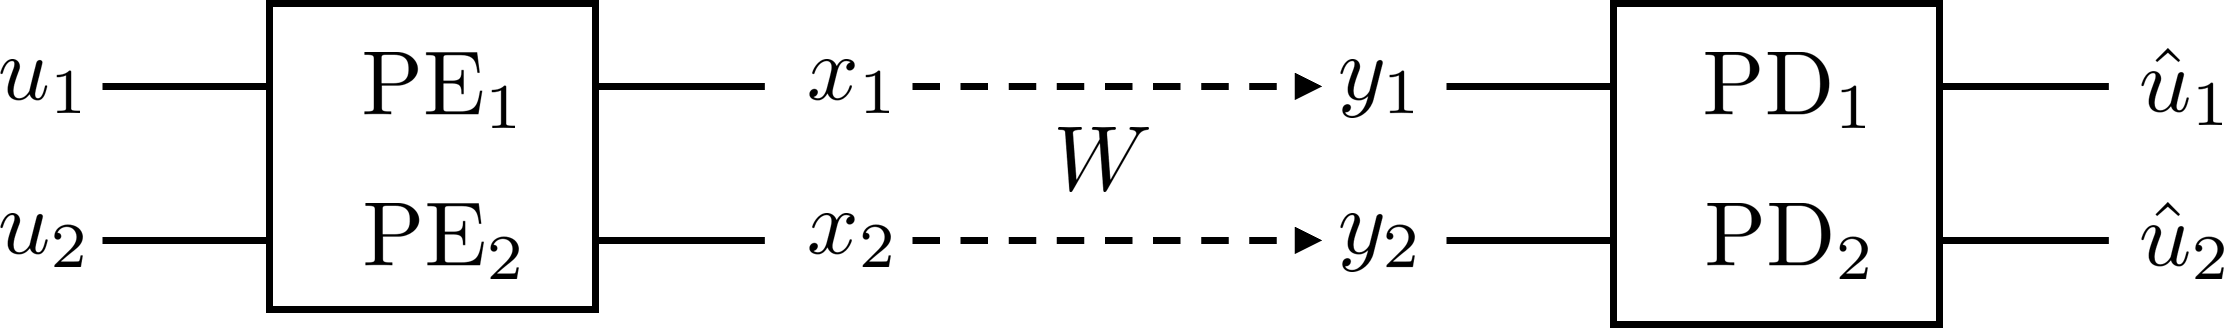
\includegraphics[width=0.6\linewidth]{figures/w2_split_channel.png}
    \caption{A single block for polar code encoding and decoding.}
\end{figure}
We have the polar encoders
\begin{equation}\begin{aligned}
    x_1\defeq \mathrm{PE}_1(u_1,u_2) &= u_1 \oplus u_2, \\
    x_2\defeq \mathrm{PE}_2(u_1,u_2) &= u_2.
\end{aligned}\end{equation}
The channel is
\begin{equation}
    W=\mathrm{BEC}(p),\; W(x)=\begin{cases}
        x &\text{w.p. } 1-p,\\
        \mathcal{E} &\text{w.p. } p.
    \end{cases}
\end{equation}
The polar decoders are
\begin{equation}\begin{aligned}
    \hat{u}_1\defeq \mathrm{PD}_1(y_1,y_2) &= \begin{cases}
        y_1 \oplus y_2 &\text{if $y_1\neq\mathcal{E}$ and $y_2\neq\mathcal{E}$}, \\
        \mathcal{E} &\text{otherwise;}
    \end{cases} \\
    \hat{u}_2\defeq \mathrm{PD}_2(y_1,y_2,u_1) &= \text{best guess of $u_2$}= \begin{cases}
        y_2 &\text{if $y_2\neq\mathcal{E}$,}\\
        y_1\oplus u_1 &\text{if $y_1\neq\mathcal{E}$ and $y_2=\mathcal{E}$,}\\
        \mathcal{E} &\text{otherwise.}
    \end{cases}
\end{aligned}\end{equation}
Note that the $u_1$ used in $\mathrm{PD}_2$ is \textit{the real one}, and not an estimate. These are the magical decoders used.

\subsection{Multi-Layered Polar Code}
We can combine it to form a two-layer polar code as below:
\begin{figure}[H]
    \centering
    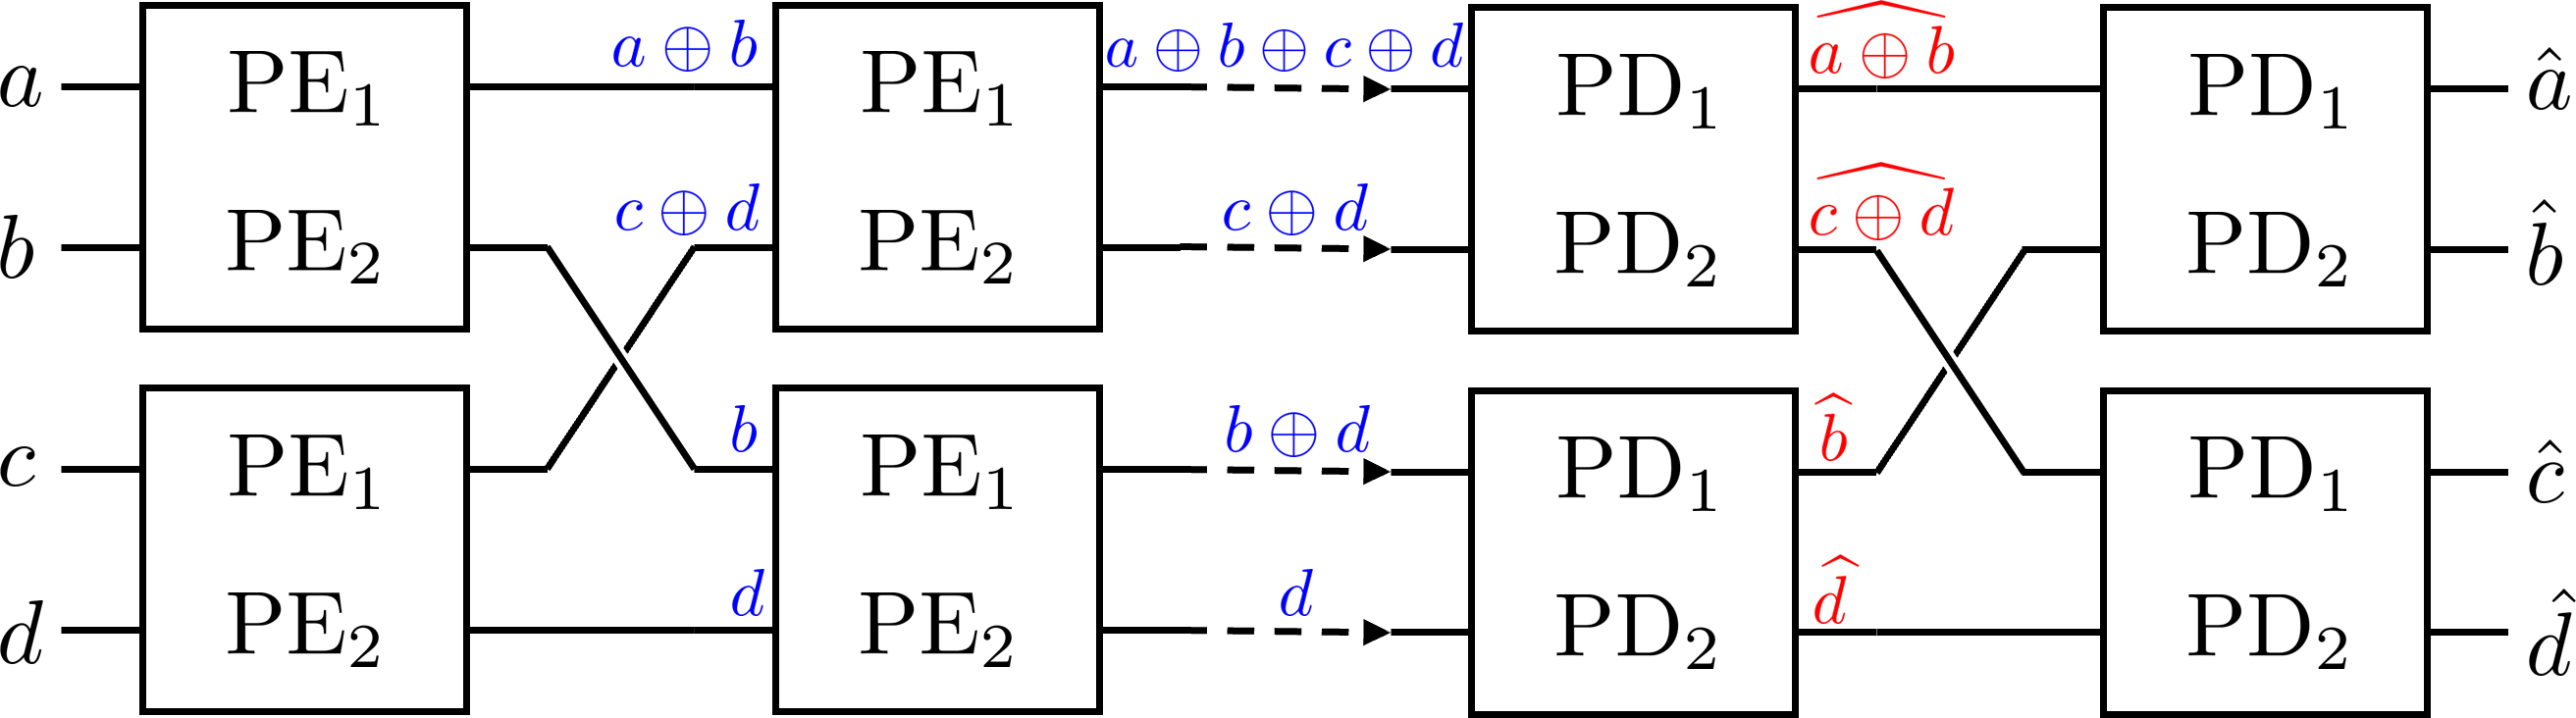
\includegraphics[width=0.7\linewidth]{figures/w2_polar_2layer.png}
    \caption{Two-layer polar code.}
\end{figure}
The variables with hats $\widehat{(\cdot)}$ once again represent estimates. On each transmission line, the variables being sent is also marked. We can further extend to a three-layer one, as shown in \autoref{fig:w2_polar_3layer}.
\begin{figure}[h]
    \centering
    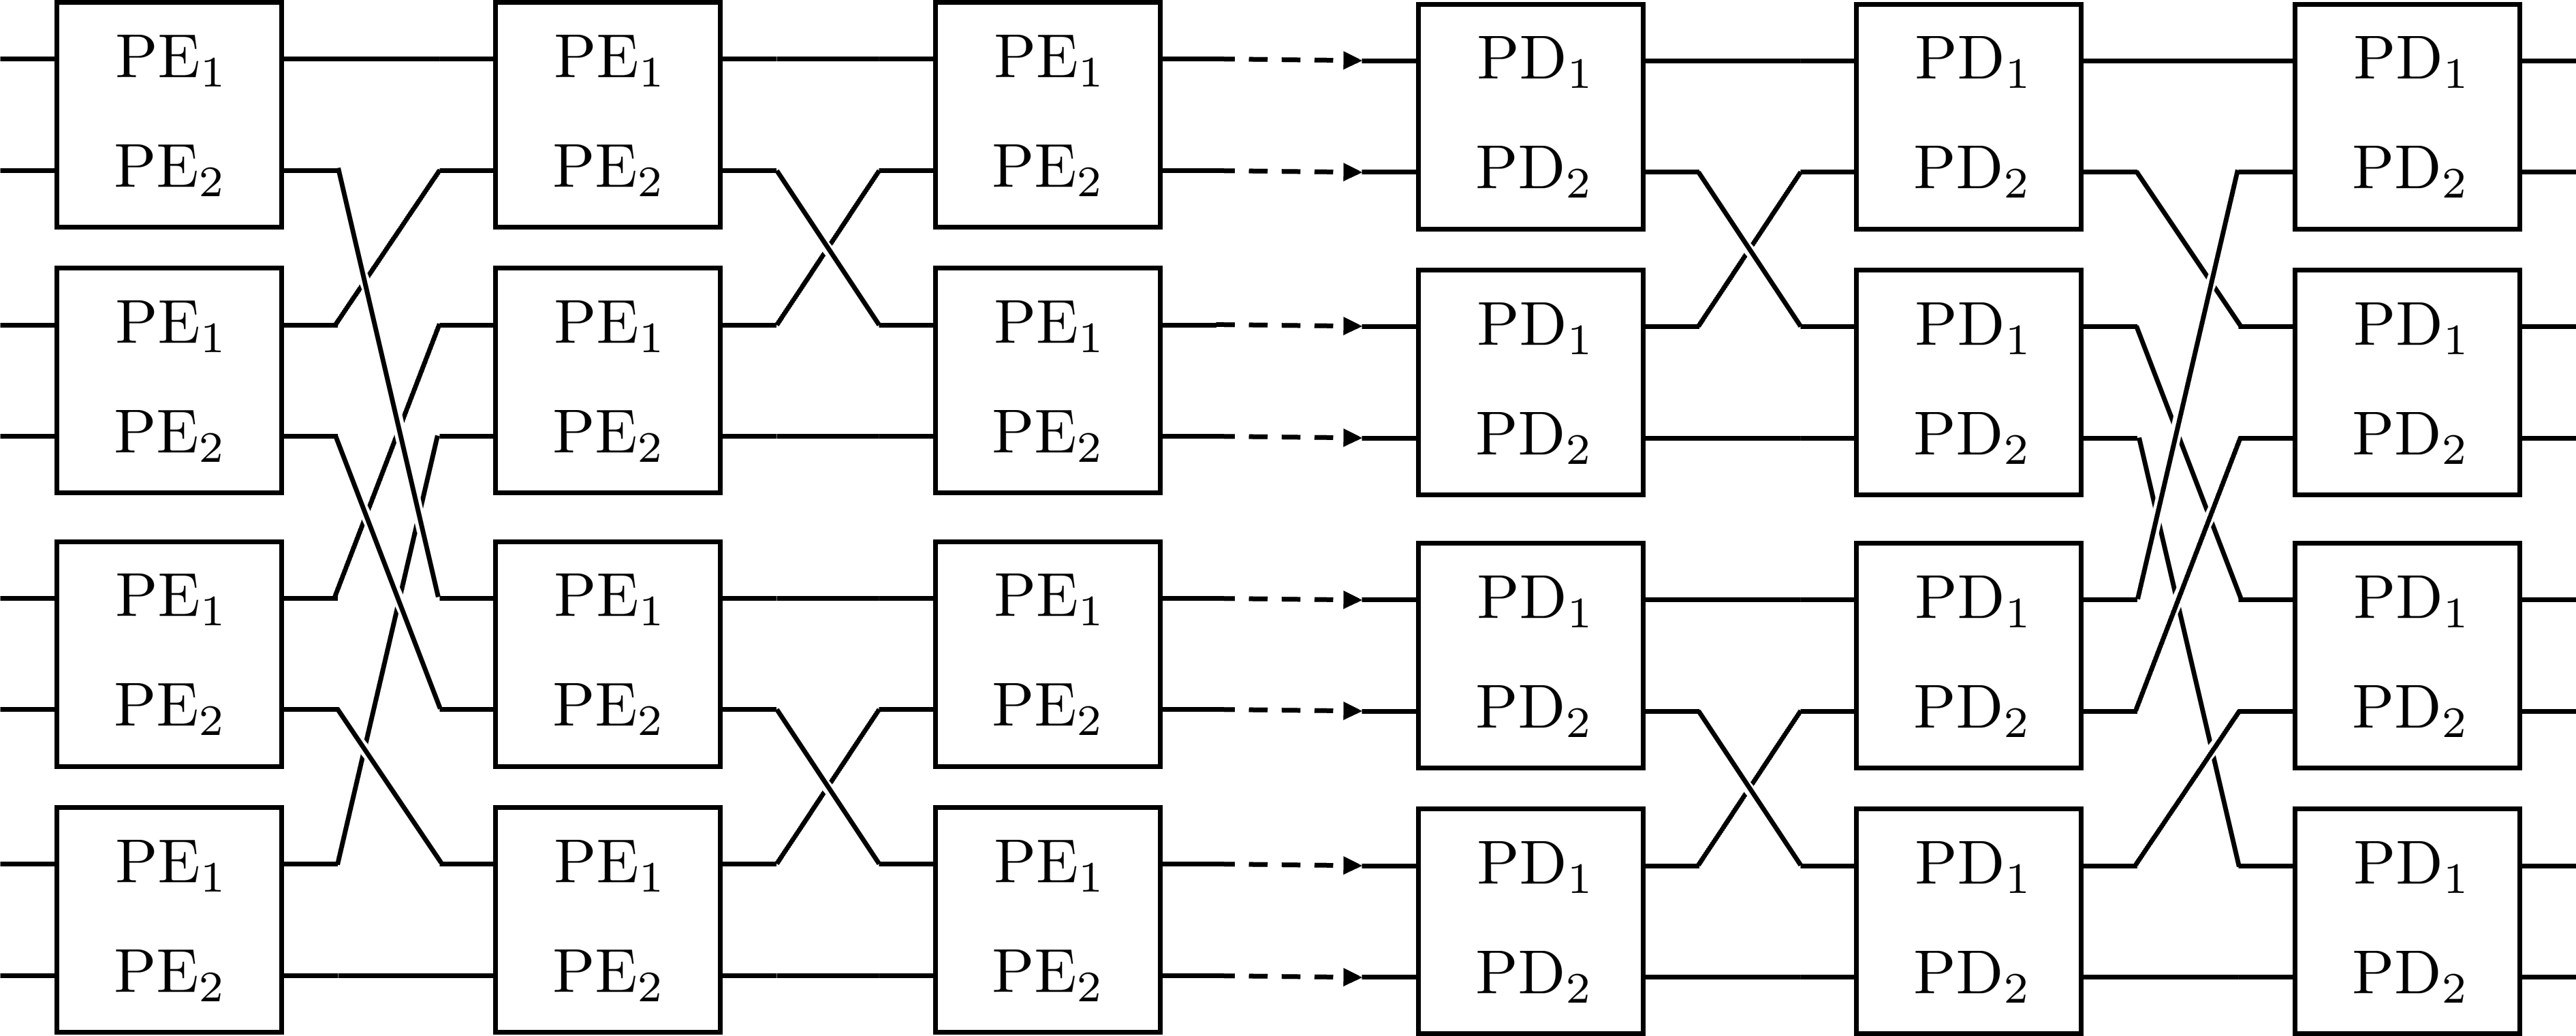
\includegraphics[width=0.8\linewidth]{figures/w2_polar_3layer.png}
    \caption{Three-layer polar code.}
    \label{fig:w2_polar_3layer}
\end{figure}
Amazingly, the structure of the encoder bears close resemblance to the \textit{butterfly diagram} used in the circuitry realization of the fast Fourier transform (FFT)! For $n$ bit inputs, the FFT algorithm has a computation complexity of $\mathrm{O}(n\lg n)$. Henceforth, the encoder structure of polar code has the operation complexity of $\mathrm{O}(n\lg n)$ as well. Random codes, on the other hand, though very useful for theoretical analysis, has a complexity of $\exp(O(n))$.

Finally, note that even though we draw the decoder also in the form of a butterfly diagram, it is not implemented so. Since $\mathrm{PD}_2$ requires the \textit{true value} to $u_1$ in calculating $\hat{u}_2$, the decoders are completed in an intertwined manner: The $\mathrm{PD}_1$'s are first calculated to obtain the required real values of $u_2$ for the $\mathrm{PD}_2$'s. As an exercise, one should check that for both the two-layer and three-layer polar code above, what is the order in which the $\mathrm{PD}_1$'s and $\mathrm{PD}_2$'s are performed? One can refer to the procedure shown in \autoref{fig:w3_polar_decoder} as a hint.

\subsection{Polar Code on BSC}
The same structure can be extended to $W=\mathrm{BSC}(p)$, the encoders can remain the same, however, the decoders need to be modified to a case-wise decision map. I.e., define the log-likelihood ratio function $\mathrm{LLR}(u\vert\theta) = \ln \left(\mathrm{Pr}\{u=0\vert\theta\} / \mathrm{Pr}\{u=1\vert\theta\}\right)$,
\begin{equation}\begin{aligned}
    \mathrm{PD}_1(y_1,y_2) &= \left[\phi\left(u_1\middle\vert\, y_1,y_2\right) \underset{1}{\overset{0}{\gtrless}} 0\right],\\
    \mathrm{PD}_2(y_1,y_2,u_1) &= \left[\phi\left(u_2\middle\vert\, y_1,y_2,u_1\right) \underset{1}{\overset{0}{\gtrless}} 0\right].
\end{aligned}\end{equation}
The value of $\phi$ needs to be determined case-wise. Even though it is more complicated than the BEC case, it still only requires finitely many steps, and hence the polar code works on BSC even in practical cases.


\section{Polar Decoder}
\lecture{4 Mar.}

As was mentioned at the end of the last section, the decoding procedure to the polar code is different from that of the encoder, and one has to go backwards and forwards between layers. The following discussion focuses on multi-layered polar codes with encoding and decoding boxes of size $2\times 2$. However, the size of encoding and decoding boxes can be $2\times2$, $3\times3$, or even $\ell\times\ell$. Please refer to Fig. 2, 3, and 4 of the paper  ``Polar Codes' Simplicity, Random Codes' Durability'' \cite{Polar_Code_Simplicity} for a more general and rigorous description of the below analysis.

\begin{figure}[h]
    \centering
    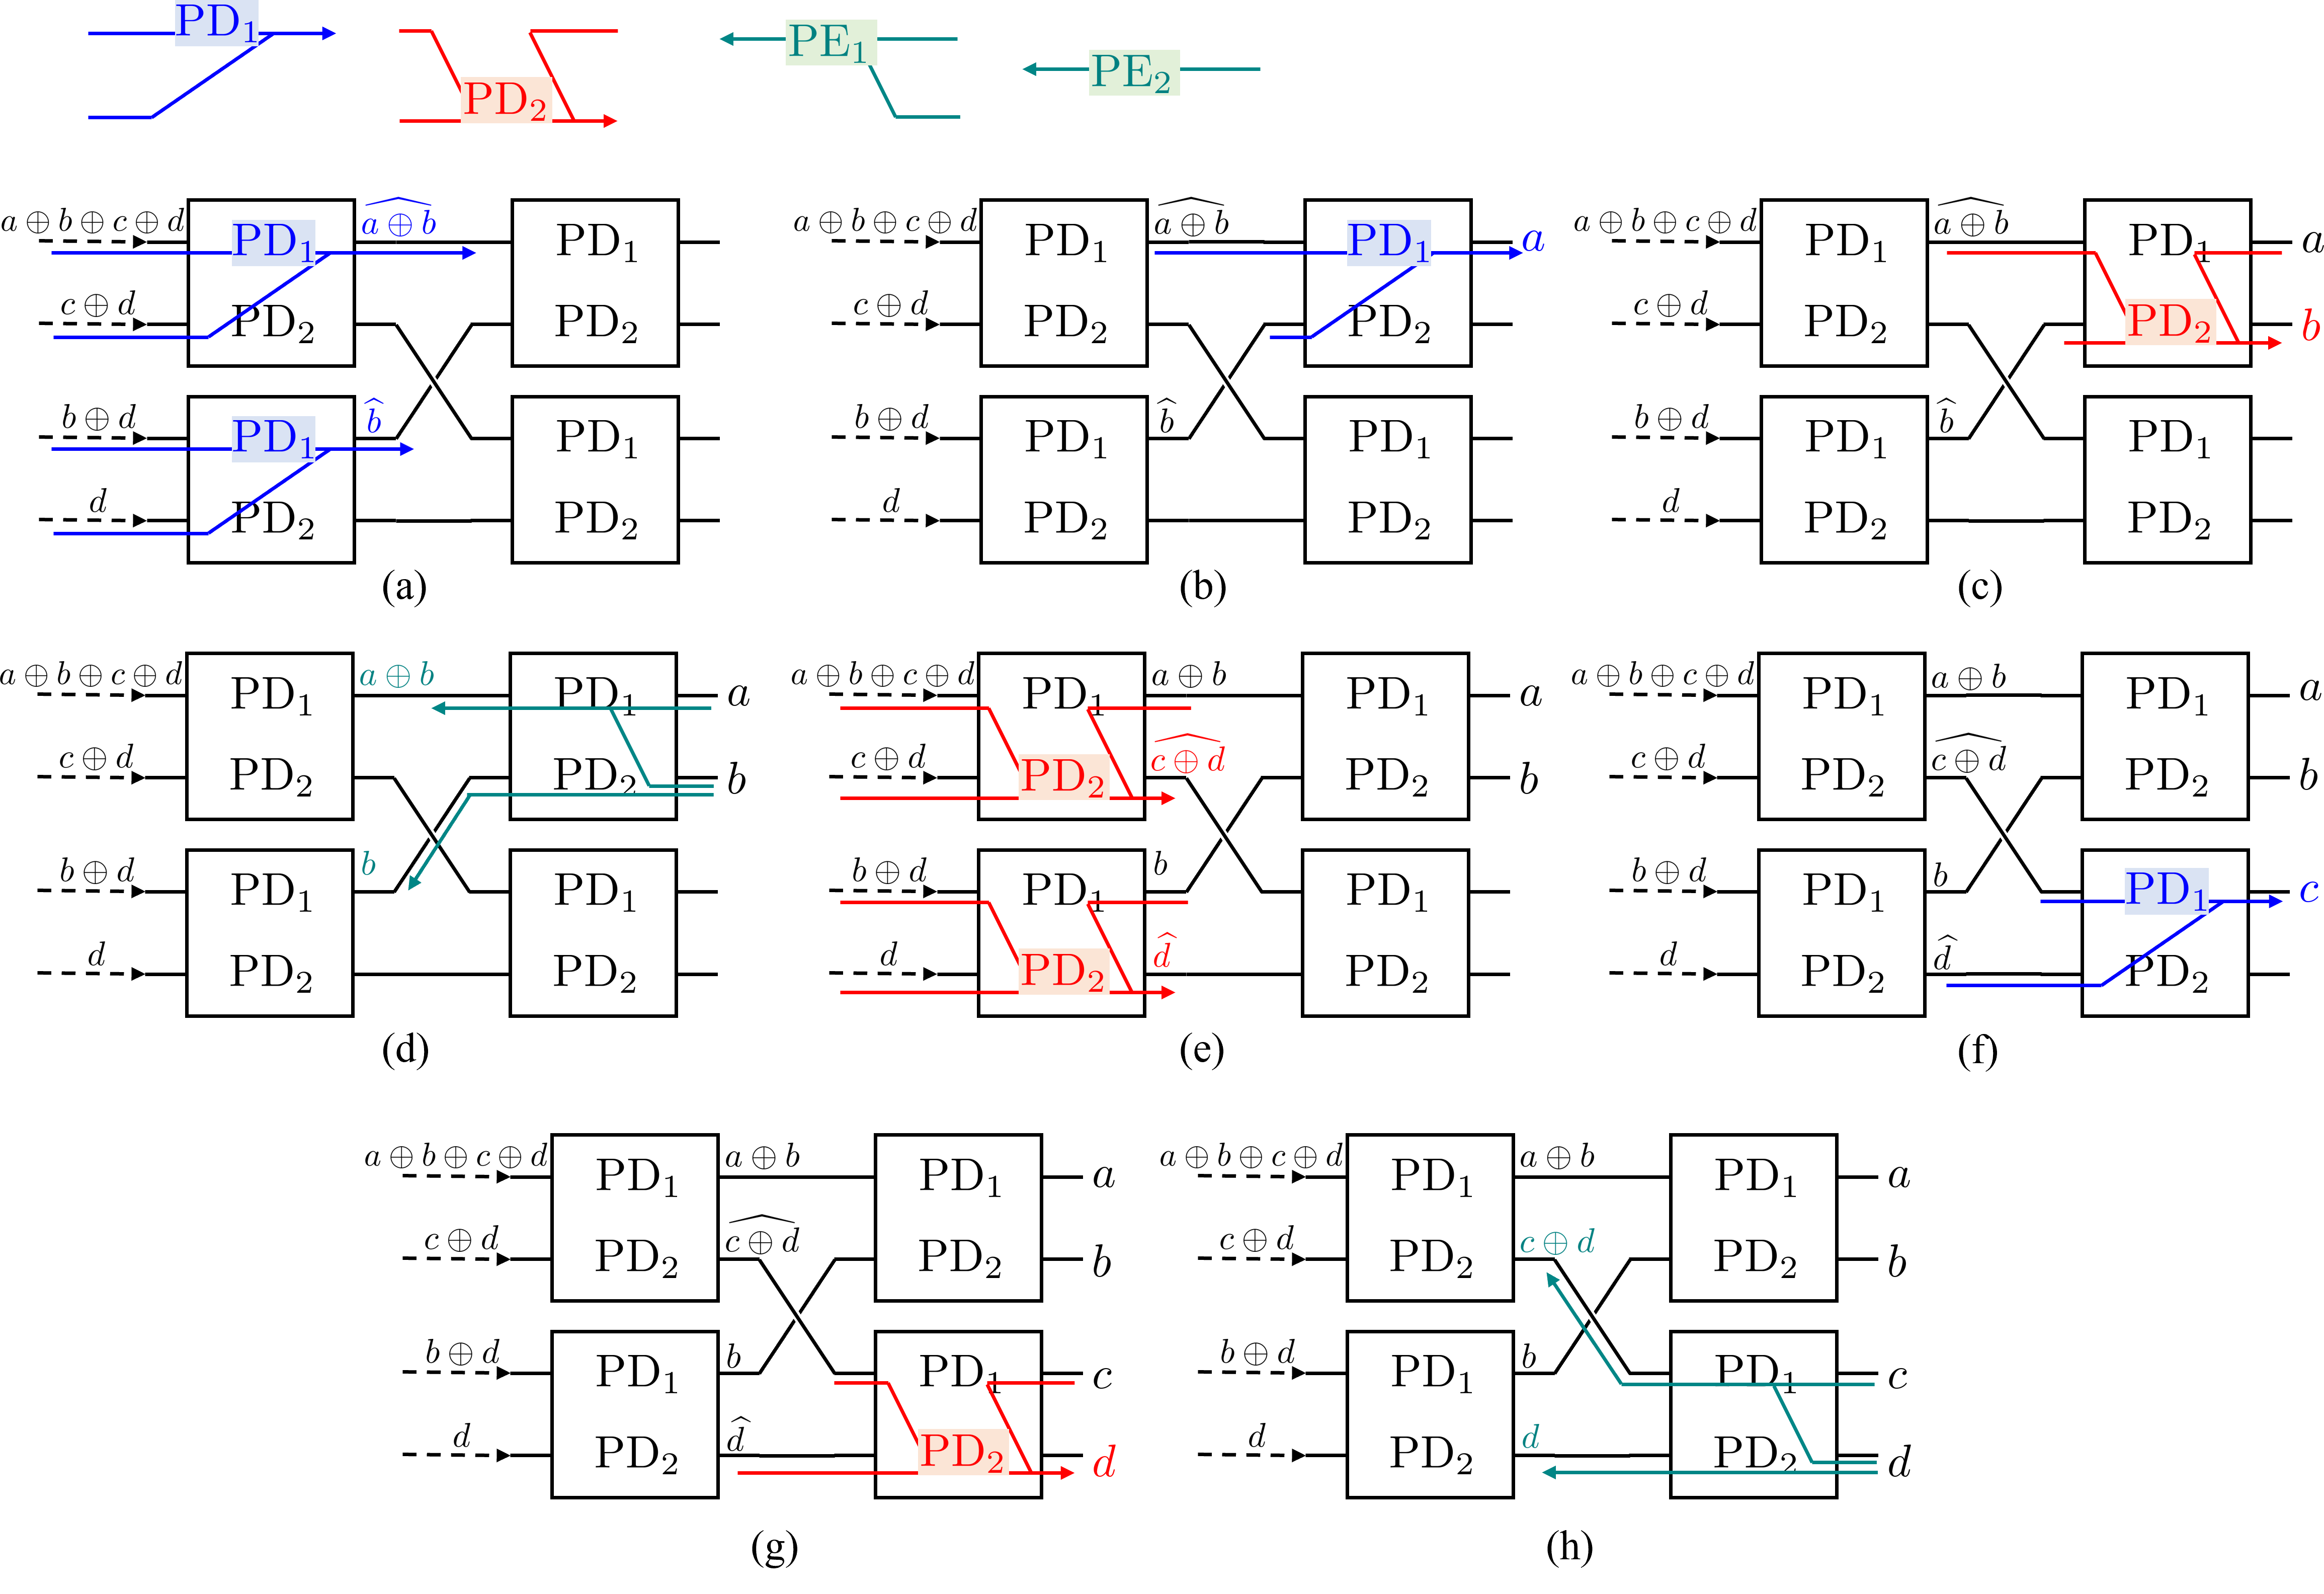
\includegraphics[width=1\linewidth]{figures/w3_2layer_decode.png}
    \caption{Decoding procedure of a two-layer polar code.}
    \label{fig:w3_polar_decoder}
\end{figure}

See the decoding procedure \autoref{fig:w3_polar_decoder} for a 2-layer polar code. Going from (a) to (h), the decoders sequentially went through the $\mathrm{PD}_1$'s and $\mathrm{PD}_2$'s. Note that since $\mathrm{PD}_2$'s require the knowledge of $u_1$'s, the box on their left will send the values by back propagating through $\mathrm{PE}_1$'s and $\mathrm{PE}_2$'s, here denoted by the teal arrows in the figure above. Moreover, we only treat the values obtained at the final column as the \textit{true} $u_1$'s.

Similar procedures can be drawn for 3-layer polar codes or more, and is left as an exercise for the readers.

The decoding of $\mathrm{PD}_2$ requires the back-propagation of true values via the polar encoders, however, what if the obtained true values are the error $\mathcal{E}$? Recall from \autoref{rmk:1.2}, it is stated that we can agree on sending $0$ over \textit{bad sub-channels} that are more erroneous. Consider having a genie\footnote{A genie is chosen since Ar{\i}kan is Turkish.} that tells us, for example, there are 4 good and 4 bad sub-channels in the 3-layer polar code as in \autoref{fig:w3_genie_aided}\footnote{What is the channel capacity implied by this distribution of good and bad channels? And no, this footnote is not an exponent.}. We can send information bits (IB) over the good sub-channels, and send frozen bits (FB) over the bad sub-channels. As mentioned, the frozen bits are chosen to be 0.

\begin{figure}[h]
    \centering
    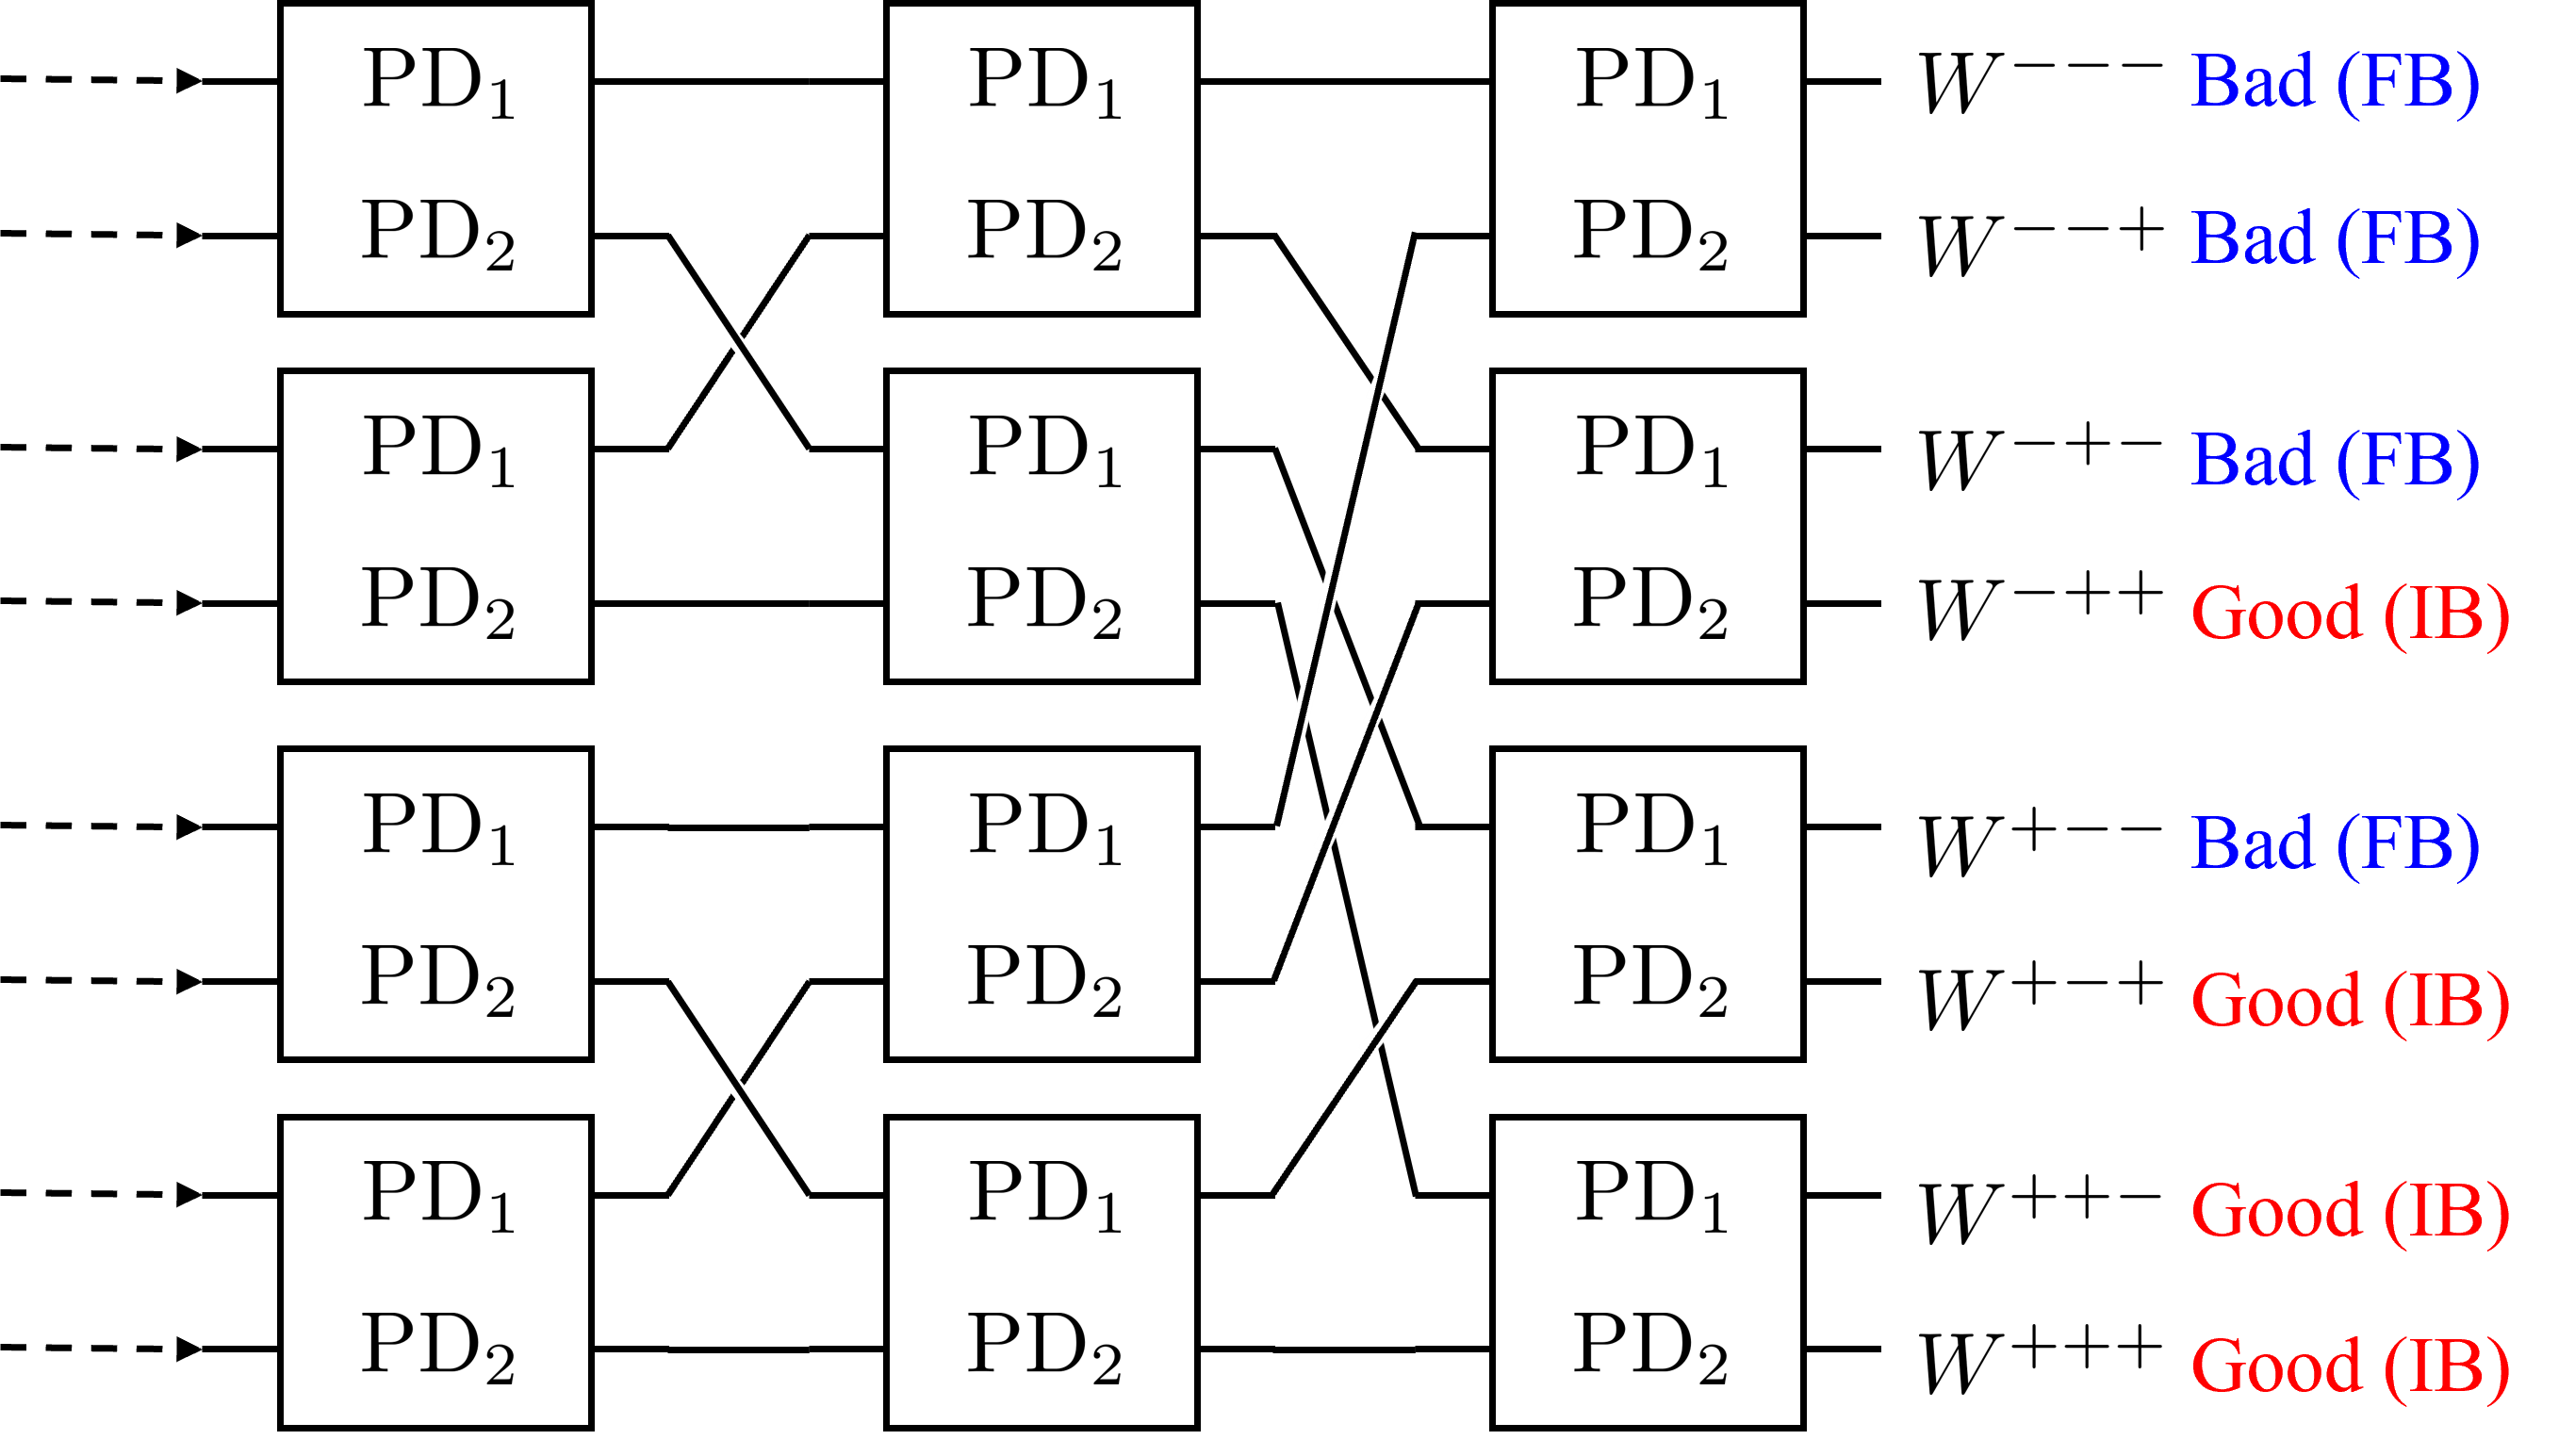
\includegraphics[width=0.6\linewidth]{figures/w3_genie.png}
    \caption{Genie-aided three-layer polar code.}
    \label{fig:w3_genie_aided}
\end{figure}

During decoding, the genie will simply send back 0 for the frozen bits as their true values; the genie will ask the decoders to figure out the true values to the information bits. One should ask themselves: why is the assignment of good and bad not \textit{continuous}? How are they determined?

Let us analyze the error probability under this scenario over BEC. Since the frozen bits can never be wrong, everything that could go wrong is when the genie gets an information bit wrong, and we simply throw out the entire block of code. The error probability will hence be: denote the polarized channels by $W^4=W^{-++}$, $W^6=W^{+-+}$, $W^7=W^{++-}$, and $W^8=W^{+++}$,
\begin{equation*}\begin{aligned}
    P_e =\; &\mathrm{Pr}\{W^{4}\text{ is wrong}\} + \mathrm{Pr}\{W^{6}\text{ is wrong}\,;\,W^{4}\text{ is right}\} \\&+ \mathrm{Pr}\{W^{7}\text{ is wrong}\,;\,W^{4},W^{6}\text{ are right}\} + \mathrm{Pr}\{W^{8}\text{ is wrong}\,;\,W^{4},W^{6},W^{7}\text{ are right}\}.
\end{aligned}\end{equation*}
If $W^4$ makes mistake, then everything else doesn't matter; if $W^4$ is correct but $W^6$ is wrong, then everything else doesn't matter; if $W^4$ and $W^6$ is correct but $W^7$ is wrong, then everything doesn't matter; if only $W^8$ is wrong, then the block is still discarded. This is also a result from the fact that the polar code is decoded sequentially. Note that from \autoref{eq:w1_bec+} and \autoref{eq:w1_bec-}, we have
\begin{equation*}
    P_e = \left((2x-x^2)^2\right)^2 + (2x^2-x^4)^2 + (2x^4-x^8) + (x^8).
\end{equation*}

The above analysis evidently shows why we choose $W^{-++}$ as a good sub-channel over $W^{+--}$.
\begin{remark}
    We choose $W^{-++}$ over $W^{+--}$ due to the fact that
    \begin{equation}
        P_e(W^{-++}) = \left((2x-x^2)^2\right)^2 \le 2(2x-x^2) - (2x-x^2)^2 = P_e(W^{+--})\;\;\;\;\;\forall\, x\in[0,1],
    \end{equation}
    with equality satisfied only at the extremals 0 and 1. See the illustration below for a clearer idea of the inequality.
    \begin{figure}[H]
        \centering
        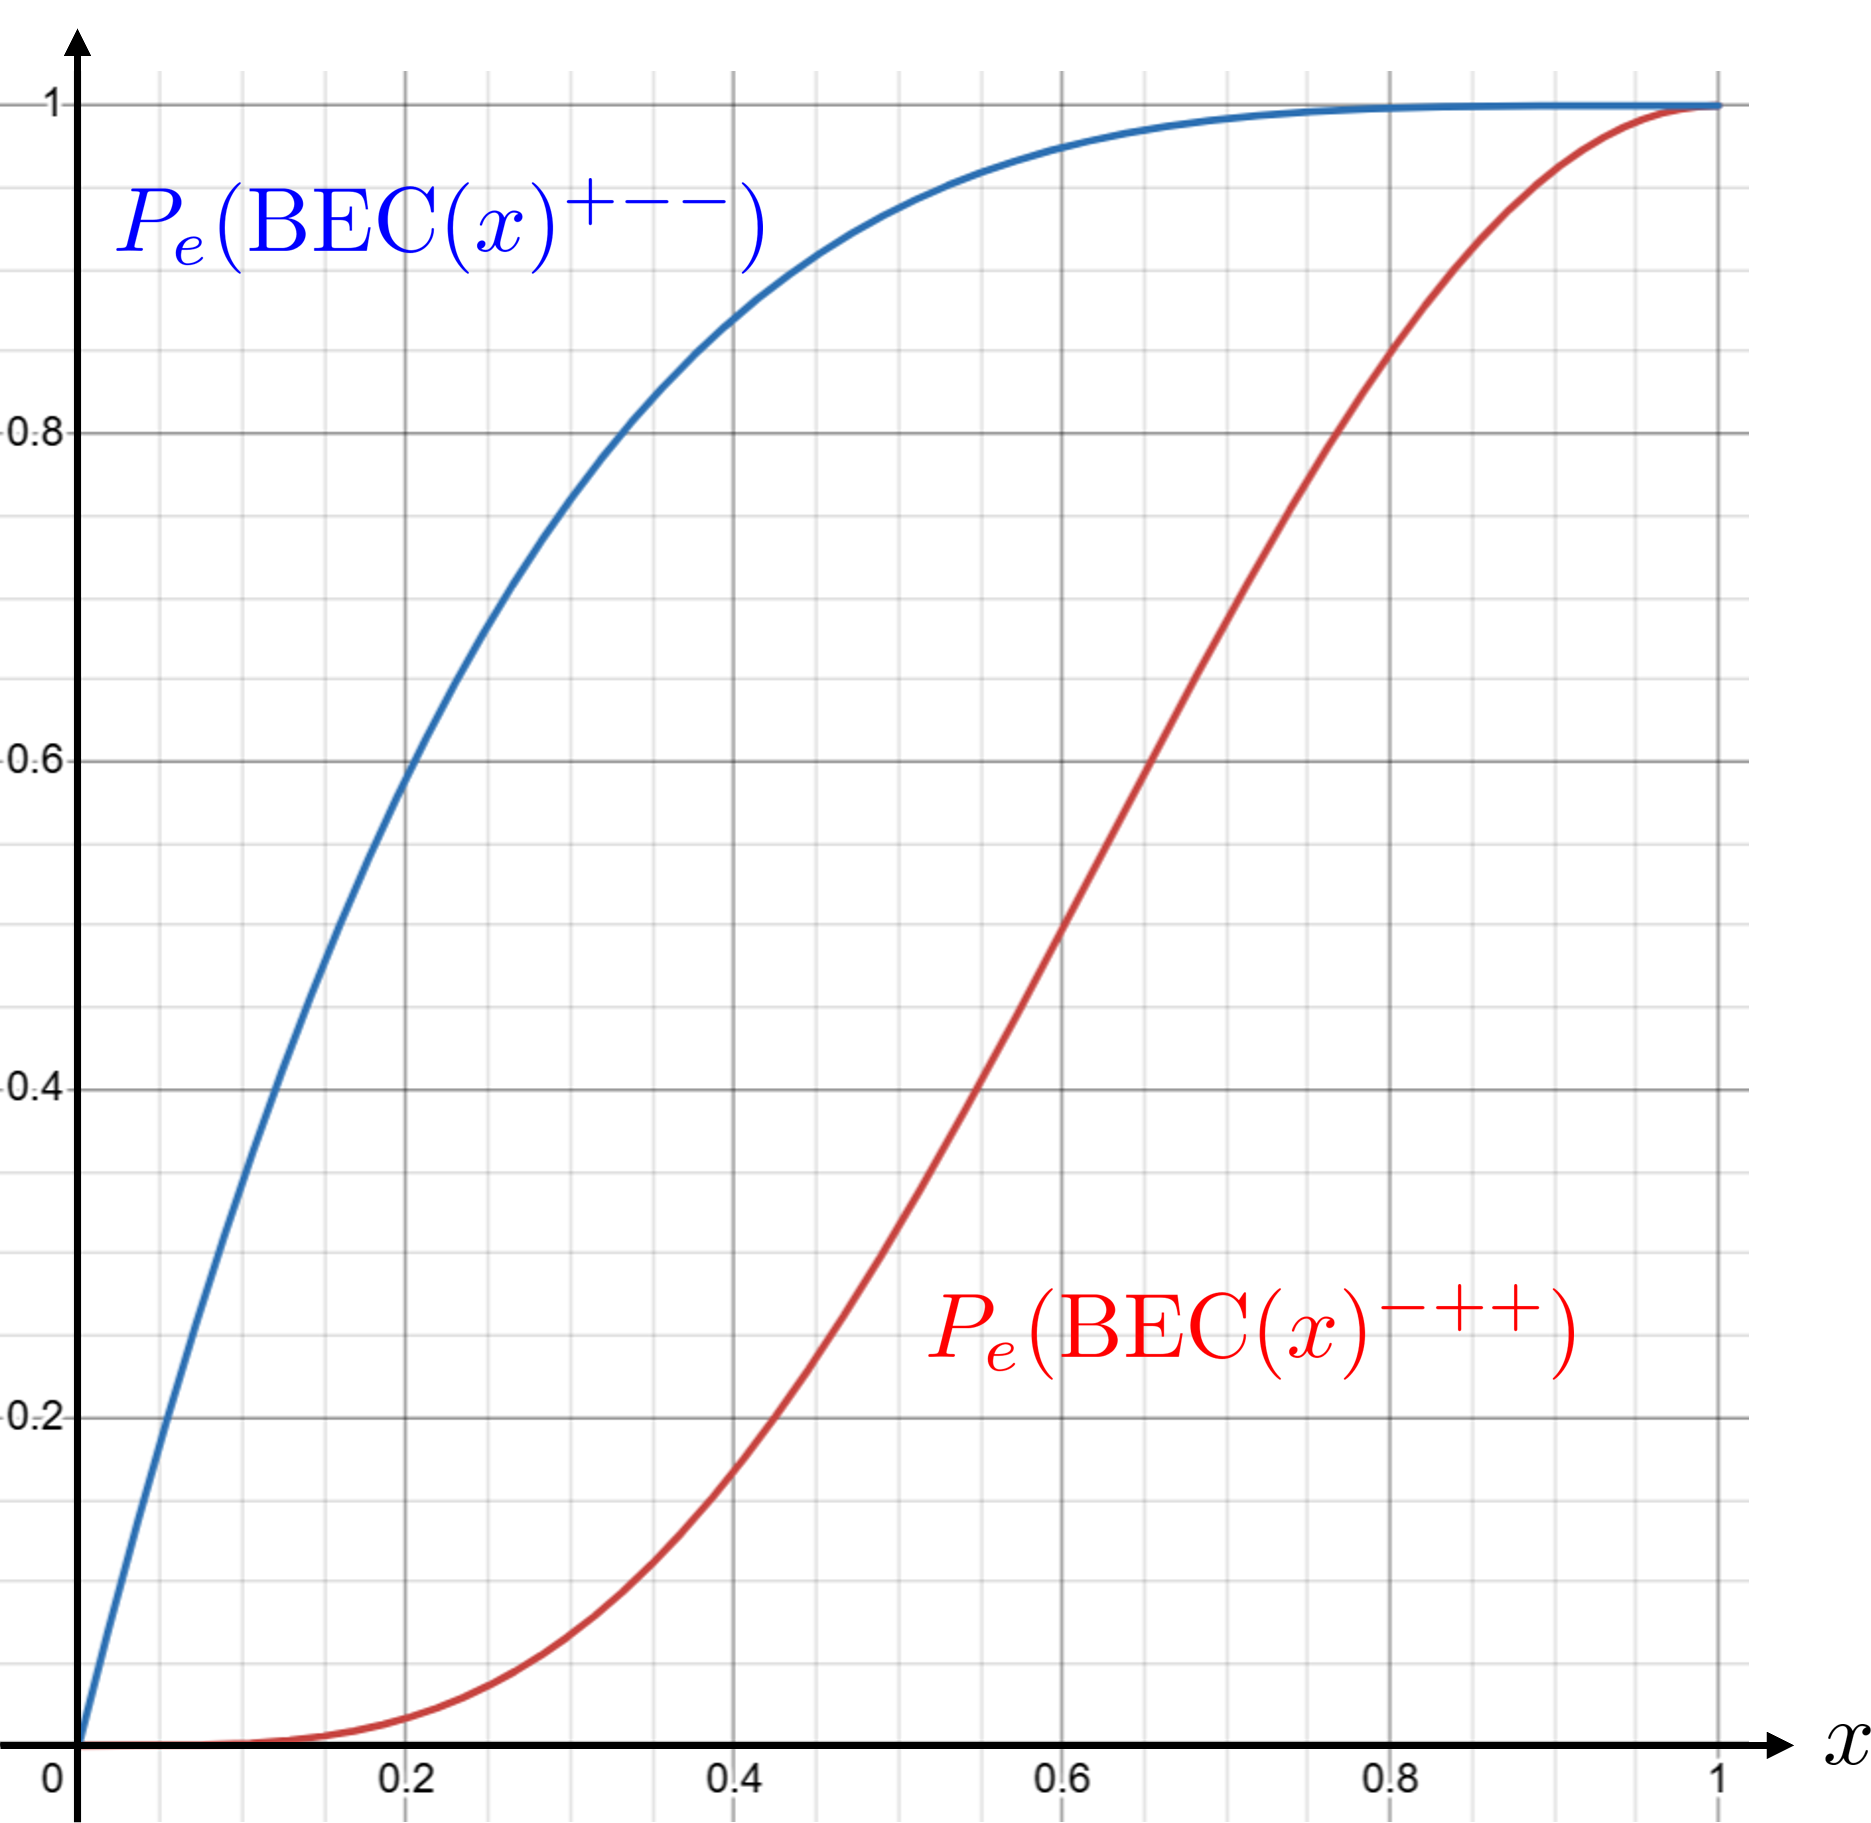
\includegraphics[width=0.35\linewidth]{figures/w3_partial_order.png}
        \caption{Ordering of the polarized error probabilities.}
    \end{figure}

    For 2-, 3-, and 4-layer polar codes over $\mathrm{BEC}(x)$, a total ordering of the sub-channels via their error probability exists.

    However, for block length greater than or equal to 32, intersections start to appear on the different error probability curves between each sub-channels. Hence, in this case, only a \textit{partial ordering} between the sub-channels exists.

    Partial-order theory is useful in deciding which sub-channel is better than which, important for the allocation of information bits, especially in the cases of long block lengths.
\end{remark}



\section{Martingale}
In this section, we take a detour and introduce the idea of a \textit{martingale}. Martingale is a special kind of random sequence that provides many useful tools from stochastic calculus in aiding our analysis of the performance of polar codes. For a proof and a more rigorous description of all the theorems below, one can refer to the book ``Probability: Theory and Examples'' \cite{Durrett} by Rick Durrett on graduate-level probability theory.

\subsection{A Brief Overview of Martingale Theory}
\begin{definition}[Martingale]
    A sequence of random variables $\{M_t\}_t$ is termed a martingale if
    \begin{align}
        &\mathbb{E}\left[\abs{M_t}\right]<\infty,&\mathbb{E}[M_{t+1}\vert M_t] = M_t.
    \end{align}
\end{definition}

Some examples of a martingale is shown below:
\begin{figure}[H]
    \centering
    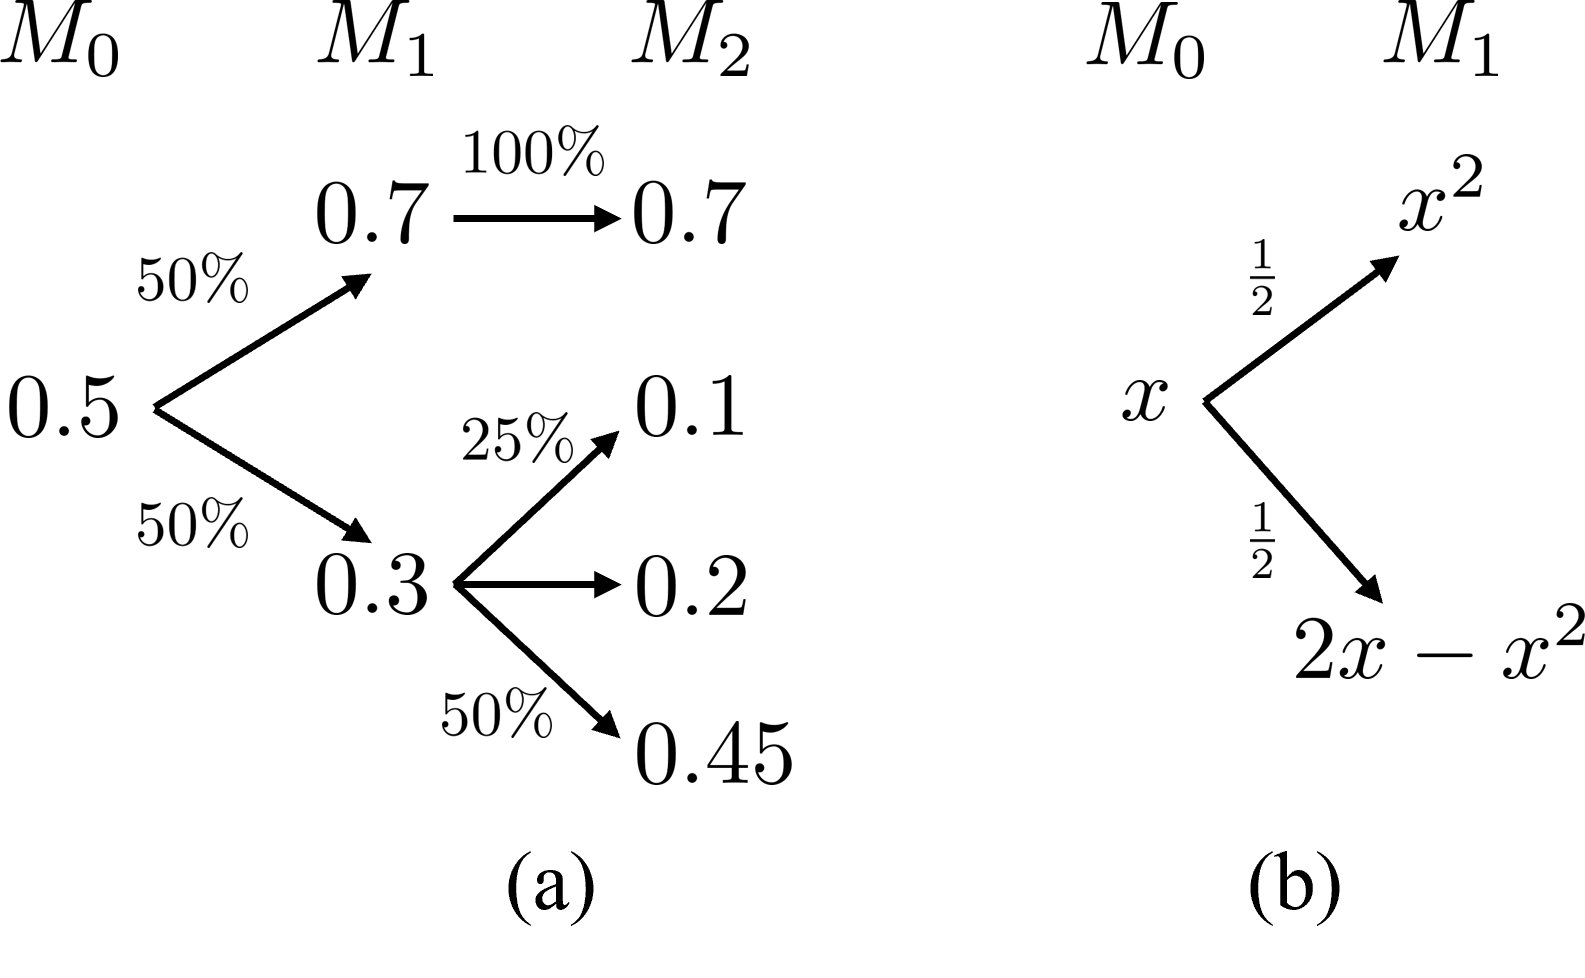
\includegraphics[width=0.5\linewidth]{figures/w3_martingale.png}
    \caption{Illustration of martingales.}
\end{figure}
One should observe that the last example given above is exactly that of the division of a BEC!

\begin{remark}
    The word ``martingale'' comes from J. Doob, the founding father of the theory of martingales. It is inspired a piece of horse gear: \textit{a long leather belt that bifurcates, at one end, into two strips of the same length}. Excerpted from ``\href{https://www.jehps.net/juin2009/Mansuy.pdf}{The origin of the word martingale},'' by Roger Mansuy.
\end{remark}

Let us now introduce the readers to a few useful theorems from the theory of martingales.
\begin{theorem}[Martingale Convergence Theorem]
    For a martingale $\{M_t\}$ that is bounded, i.e., $\abs{M_t}<\infty$\footnote{The absolutely boundedness is a really strong constraint, which can be relaxed to bounded absolute expectation.}, there exists a random variable $M_\infty$ such that $M_t\xrightarrow{\text{a.s.}} M_\infty$ as $t\rightarrow\infty$.
\end{theorem}

Here we shall give a more illustrative example showing that the theorem above is reasonable and should instinctively hold:
\begin{example}
    Define $\{M_t\}$ as the \textit{polarization process} of polar code over BEC. Let $M_0 = x$, with
    \begin{equation}
        M_{t+1} = \begin{cases}
            M_t^2 &\text{w.p. }\frac{1}{2},\\
            2M_t-M_t^2 &\text{w.p. }\frac{1}{2}.
        \end{cases}
    \end{equation}
    By the theorem above, $M_\infty$ should exist, and we further claim that $M_\infty\in\{0,1\}$.

    If $\mathrm{Pr}\left\{M_\infty=x\neq\{0,1\}\right\}\ge0$, then for all $t\ge T$, there exists a $T\gg0$ such that $M_t\in[x-\varepsilon,x+\varepsilon]$ for some fixed $\varepsilon>0$. However, $M_{T+1}$, there are 50\% chances that either of the following happens:
    \begin{align*}
        M_T^2 &\le (x+\varepsilon)^2 < x-\varepsilon,\\
        2M_T-M_T^2 &\ge 2(x-\varepsilon)-(x-\varepsilon)^2 > x+\varepsilon,
    \end{align*}
    both leading to a contradiction by choosing an $\varepsilon$ small enough. The claim that $M_\infty\in\{0,1\}$ is thus proven by contradiction.
\end{example}

\begin{example}
    Again consider $\{M_t\}$ as the polarization process of polar code over $\mathrm{BEC}(x)$. We have
    \begin{align}
        \mathrm{Pr}\{M_\infty=1\} = \mathbb{E}[M_\infty] &= \mathbb{E}\left[\lim_{t\rightarrow\infty} M_t\right] \notag\\
        &= \lim_{t\rightarrow\infty} \mathbb{E}[M_t] \label{eq:w3_martingale}\\
        &= \lim_{t\rightarrow\infty} \mathbb{E}[M_{t-1}] = \cdots = \lim_{t\rightarrow\infty} \mathbb{E}[M_0] = x. \notag
    \end{align}
    The validity of the exchange of the limit and expectation in \autoref{eq:w3_martingale} is guaranteed by the convergence of the martingale in the limit.

    Similarly, we have $\mathrm{Pr}\{M_\infty=0\} = 1-x$.
    
    Further consider a random $s\in\{+,-\}^n$, we have
    \begin{equation}\begin{aligned} \label{eq:w3_martingale_conv}
        \mathrm{Pr}\{\mathrm{BEC}(x)^s \text{ is close to }\mathrm{BEC}(1)\} &= x, \\
        \mathrm{Pr}\{\mathrm{BEC}(x)^s \text{ is close to }\mathrm{BEC}(0)\} &= 1-x.
    \end{aligned}\end{equation}
    The number of $s\in\{+,-\}^n$ such that $\mathrm{BEC}(x)^s$ is good is $2^n(1-x-\varepsilon)$, corresponding to the number of information bits; the rest of $2^n(x+\varepsilon)$ are bad, corresponding to the frozen bits.
\end{example}


\begin{definition}[Stopping Time]
    An integer random variable $\sigma$ is called a \textit{stopping time} if whether or not $\sigma\le t$ depends only on $M_1,\ldots,M_t$, and not on $M_{t+1},M_{t+1},\ldots$.
\end{definition}
\begin{theorem}[Optional Stopping Time]
    For a martingale $\{M_t\}$ with stopping time $\sigma$, we have
    \begin{equation}
        \mathbb{E}[M_\sigma] = \mathbb{E}[M_0].
    \end{equation}
\end{theorem}
The proof can be directly seen from the example above.

\begin{example}
    Let us consider a martingale $\{M_t\}$ with $M_t\ge0$. Let $M_0=0.001$ be deterministic. Define its stopping time as $\sigma\defeq\min\setdef{t}{M_t\ge1}\cup\{N\}$ where $N$ is very large. In the context of a stock market, this definition of stopping time corresponds to ones strategy of selling out when reaching a gain of profit larger than 1 with a small initial investment. Let us bound the success probability of such strategy.
    \begin{align*}
        M_0 \equiv \mathbb{E}[M_\sigma] &= \mathbb{E}\left[M_\sigma\cdot\mathbbm{1}\{M_\sigma\ge1\}\right] + \mathbb{E}\left[M_N\cdot\mathbbm{1}\{M_\sigma\text{ is never larger than }1\}\right] \\
        &\ge \mathbb{E}\left[M_\sigma\cdot\mathbbm{1}\{M_\sigma\ge1\}\right] \\
        &\ge \mathrm{Pr}\{M_\sigma\ge1\}.
    \end{align*}
    Henceforth, we have $\mathrm{Pr}\{M_\sigma\ge1\}\le M_0=0.1\%$. The probability of gaining huge profit from small investment in this model is small.
\end{example}
This result above can be generalized via the Markov inequality: given a martingale $M_t\ge0$, we have $\mathrm{Pr}\{M_\sigma\ge a\} \le \mathbb{E}[M_\sigma]/a = \mathbb{E}[M_0]/a$. This is known as Doobs's maximum inequality.
\begin{theorem}[Doob's Maximum Inequality]
    Let the optional stopping time for a martingale $\{M_t\}$ be
    \begin{equation}
        \sigma:\text{ minimum }t\text{ that }M_t\text{ reaches }A.
    \end{equation}
    Then since
    \begin{equation}
        M_\sigma \ge A \Leftrightarrow \max_t M_t \ge A,
    \end{equation}
    we have
    \begin{equation}
        \mathrm{Pr}\{\max_t M_t\ge A\} = \mathrm{Pr}\{M_\sigma\ge A\} \le \frac{M_0}{A}.
    \end{equation}
\end{theorem}
\begin{remark}
    Doob single-handedly translated the theory of martingale from a competing theory of description of probability to the now widely-used measure-theoretical probability theory.
\end{remark}
\begin{remark}
    The applications to martingale often includes stochastic calculus and stock market analysis. The concept of stopping time can be, as an example, interpreted as the time one sells out their stocks.

    Moreover, two other kinds of martingales exist:
    \begin{enumerate}
        \item Supermartingale: $\mathbb{E}[M_{t+1}\vert M_t] \le M_t$;
        \item Submartingale: $\mathbb{E}[M_{t+1}\vert M_t] \ge M_t$.
    \end{enumerate}
\end{remark}

We can proof the (Doob's) martingale convergence theorem from the Doob's maximum inequality:
\begin{proof}
    Assume that we are considering a bounded martingale $0\le M_t\le 1$. We claim that if $M_t$ does not converge, then there exists $0< a<b<1$ such that $M_t$ oscillates infinitely many times between $a$ and $b$. See the figure below:
    \begin{figure}[H]
        \centering
        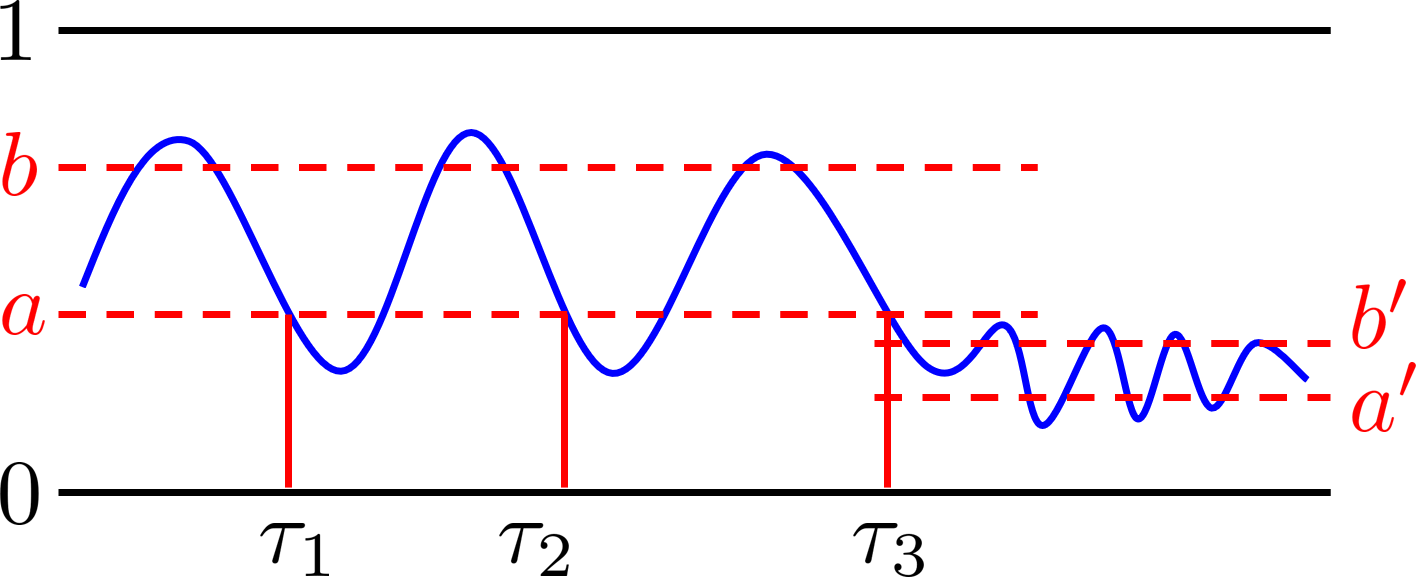
\includegraphics[width=0.5\linewidth]{figures/w4_martingale_oscillate.png}
        \caption{Illustration of the martingale convergence theorem.}
    \end{figure}
    If the martingale oscillates outside $[a,b]$, one can find another interval $[a',b']$ in which the martingale will finally reside in. Denote the time when $M_t=a$ as $\tau$'s, we have, from the maximum inequality:
    \begin{equation}
        \mathrm{Pr}\{M_{\tau+t}\ge b\vert M_\tau=a\} \le \frac{a}{b} <1.
    \end{equation}
    Since the oscillation happens infinitely many times, we have the total probability $(\frac{a}{b})^n\rightarrow 0$. Thus, if the sequence doesn't bound between 2 numbers, it must be \textit{almost surely} convergent.
\end{proof}

\subsection{McDiarmid's Inequality}
Recall from large deviation theory that we have, for i.i.d. and bounded random variables $X_1$, $\ldots$, $X_n$,
\begin{equation}
    \mathrm{Pr}\left\{\frac{X_1+\cdots+X_n}{n} - \mathbb{E}[X_1] \ge \varepsilon\right\} \le \exp(-c\varepsilon^2n)
\end{equation}
for some constant $c$. This is known as the Chernoff bound or Hoeffding's inequality.

A similar version for martingale exists:
\begin{theorem}[Azuma's Inequality]
    For a martingale $\{M_t\}$ with bounded variation $\abs{M_{t+1}-M_t}\le C$, we have
    \begin{equation}
        \mathrm{Pr}\left\{\frac{M_n}{n}-M_0 > \varepsilon\right\} < \exp(-c\varepsilon^2n)
    \end{equation}
    for some constant $c$.
\end{theorem}
This inequality can be used to show the capacity-achieving property of polar codes. Moreover, by defining $M_t$ as
\begin{equation}
    M_t \defeq X_1+\cdots+X_t - t\cdot\mathbb{E}[X_1],
\end{equation}
we can see that it is indeed a martingale:
\begin{equation*}
    \mathbb{E}[M_{t+1}\vert M_t] = M_t + \mathbb{E}\left[X_{t+1}-\mathbb{E}[X_1]\right] = M_t.
\end{equation*}
We readily obtained the Hoeffding's inequality from Azuma's inequality.

This result can, obviously, be further generalized. Let us define some similar notions needed for the description of the following theorem.
\begin{definition}[Bounded Variation]
    A function $f:[0,1]^n\rightarrow \mathbb{R}$ is of bounded variation if there exists a $C_i$ such that
    \begin{equation}
        \abs{f(a_{1:i-1},b_i,a_{i+1:n}) - f(a_{1:i-1},c_i,a_{i+1:n})} < C_i
    \end{equation}
    is satisfied for all possible $i$, $b_i$, and $c_i$.
\end{definition}
\begin{definition}[Doob's Martingale]
    For an $n$-variable function $f$, the following sequence is a martingale:
    \begin{align}
        M_0 &= \mathbb{E}_Y[f(Y_{1:n})], \\
        M_t &= \mathbb{E}_{Y_{t+1:n}}[f(X_{1:t},Y_{t+1:n})], \\
        M_n &= f(X_1,\ldots,X_n).
    \end{align}
\end{definition}
\begin{theorem}[McDiarmid's Inequality]
    For $f$ of bounded variation, there exists $L$ such that
    \begin{equation}
        \mathrm{Pr}\{f(X_{1:n}) - L > \varepsilon\} < \exp(-c\varepsilon^2n).
    \end{equation}
\end{theorem}
The McDiarmid's inequality is often used in statistical learning, where $X_{1:n}$ can be seen as a random data set obtained. All in all, both Azuma's and McDiarmid's inequality show the concentration of bounded-variational martingales or functions, respectively.

\subsection{Analyzing Polar Code over BEC via Martingale}
This subsection utilizes our newly obtained skills from the martingale theory to apply to an example of polar code over BEC.

\begin{example}
    Let us construct a $2n$-layer polar code (with block length being $2^{2n}=4^n$) over $\mathrm{BEC}(x)$ with $x$ small. Let us define the set
    \begin{equation*}
        \mathcal{A} \defeq \setdef{s\in\{+,-\}^n}{P_e\left(\mathrm{BEC}(x)^s\right) < 2^{-10}}.
    \end{equation*}
    For a fixed sub-channel $s\in\mathcal{A}$, we further pick a random $t\in\{+,-\}^n$. One should be immediately be curious of the bound to
    \begin{equation*}
        \mathrm{Pr}\left\{P_e\left(\mathrm{BEC}(x)^{st_{1:j}}\right) \ge 2^{-6}\right\},
    \end{equation*}
    where $st_{1:j}$ is the concatenation of the string $s$ with $t_{1:j}$, the first to $j$th element of $t$.
    
    By the optional stopping time theorem in the previous subsection, we have that
    \begin{equation*}
        \mathrm{Pr}\left\{P_e\left(\mathrm{BEC}(x)^{st_{1:j}}\right) \ge 2^{-6}\right\} \le 2^{-10}\cdot 2^{6} = 2^{-4} \;\;\;\;\;\text{for some stopping time $j$.}
    \end{equation*}
    
    Next, let
    \begin{equation*}
        \mathcal{B} \defeq \setdef{st\in\{+,-\}^{2n}}{s\in\mathcal{A},\; P_e\left(\mathrm{BEC}(x)^{st} \le 2^{-6}\right) \text{ for fixed }s}.
    \end{equation*}
    What will $\abs{\mathcal{B}} / \left(2^n\abs{\mathcal{A}}\right)$ be? It is easy to see that
    \begin{equation*}
        \frac{\abs{\mathcal{B}}}{2^n\abs{\mathcal{A}}} \ge 1-2^{-4}.
    \end{equation*}
    
    For an $st\in\mathcal{B}$, every new $+$ sign sends $x$ to $x^2$; and every new $-$ sign send $x$ to $2x$ (since $x$ is assumed to be small, the term $-x^2$ is omitted). One further asks that, for example, if $t$ contains at least $n/3$ $+$'s and at most $2n/3$ $-$'s, what is the error probability $P_e\left(\mathrm{BEC}(x)^{st}\right)$?
    
    We can bound it by considering the variables
    \begin{equation}\begin{aligned}
        a_0 &\defeq \lg\left(-\lg P_e\left(\mathrm{BEC}(x)^s\right)\right), \\
        a_j &\defeq \lg\left(-\lg P_e\left(\mathrm{BEC}(x)^{st_{1:j}}\right)\right),
    \end{aligned}\end{equation}
    satisfying the following recursion relation:
    \begin{equation}
        a_{j+1} = \begin{cases}
            a_j + 1 &\text{if }t_{j+1}=+, \\
            a_j - \varepsilon_k &\text{if }t_{j+1}=-.
        \end{cases}
    \end{equation}
    Then we have that $a_n\ge\frac{n}{3} - (\max_k\varepsilon_k)\frac{2n}{3} = rn$ for a constant $r$. Thus, for an $st\in\mathcal{B}$, the error probability has a bound
    \begin{equation*}
        P_e\left(\mathrm{BEC}(x)^{st}\right) < 2^{-2^{rn}} \text{ w.p. }\mathrm{Pr}\left\{\text{a random $t$ has $\ge \frac{n}{3}$ of +'s}\right\} \ge 1-\ee^{-cn},
    \end{equation*}
    for some constant $c$ derived from the Chernoff bound. The Chernoff bound is applicable since $\frac{n}{3}\le \frac{n}{2} = \mathbb{E}[\text{\# of $+$'s in a random $t$}]$. Lastly, the number of $st\in\{+,-\}^{2n}$ subject to $P_e\left(\mathrm{BEC}(x)^{st}\right)<2^{-2^{rn}}$ is greater than $2^n\abs{\mathcal{A}} - 2^{2n}\left(2^{-4} - \exp(-cn)\right)$.
\end{example}

\section{Polar Code over BSC and BMSC}
\subsection{Binary Memoryless Symmetric Channel}
Binary memoryless symmetric channel (BMSC) is a generalization to BSC.
\begin{definition}[BMSC]
    A channel $W:\{0,1\}\rightarrow\mathcal{Y}$ with an involution $\iota:\mathcal{Y}\rightarrow\mathcal{Y}$ (an involution is a permutation that satisfies $\iota^2=\mathrm{identity}$) is called a BMSC if
    \begin{equation}
        W(y\vert0) = W(\iota(y)\vert 1).
    \end{equation}
\end{definition}

Some prime examples of a BMSC are BSC and BEC. The figure below shows another example of a BMSC and its involution.
\begin{figure}[H]
    \centering
    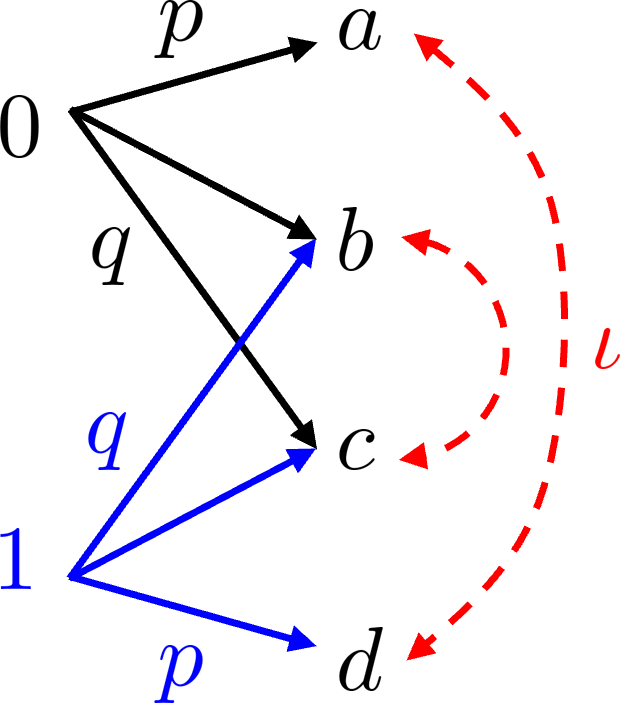
\includegraphics[width=0.2\linewidth]{figures/w3_BMSC.png}
    \caption{Involution of a BMSC.}
\end{figure}
A more general construction of a BMSC channel is shown as follow:
\begin{figure}[H]
    \centering
    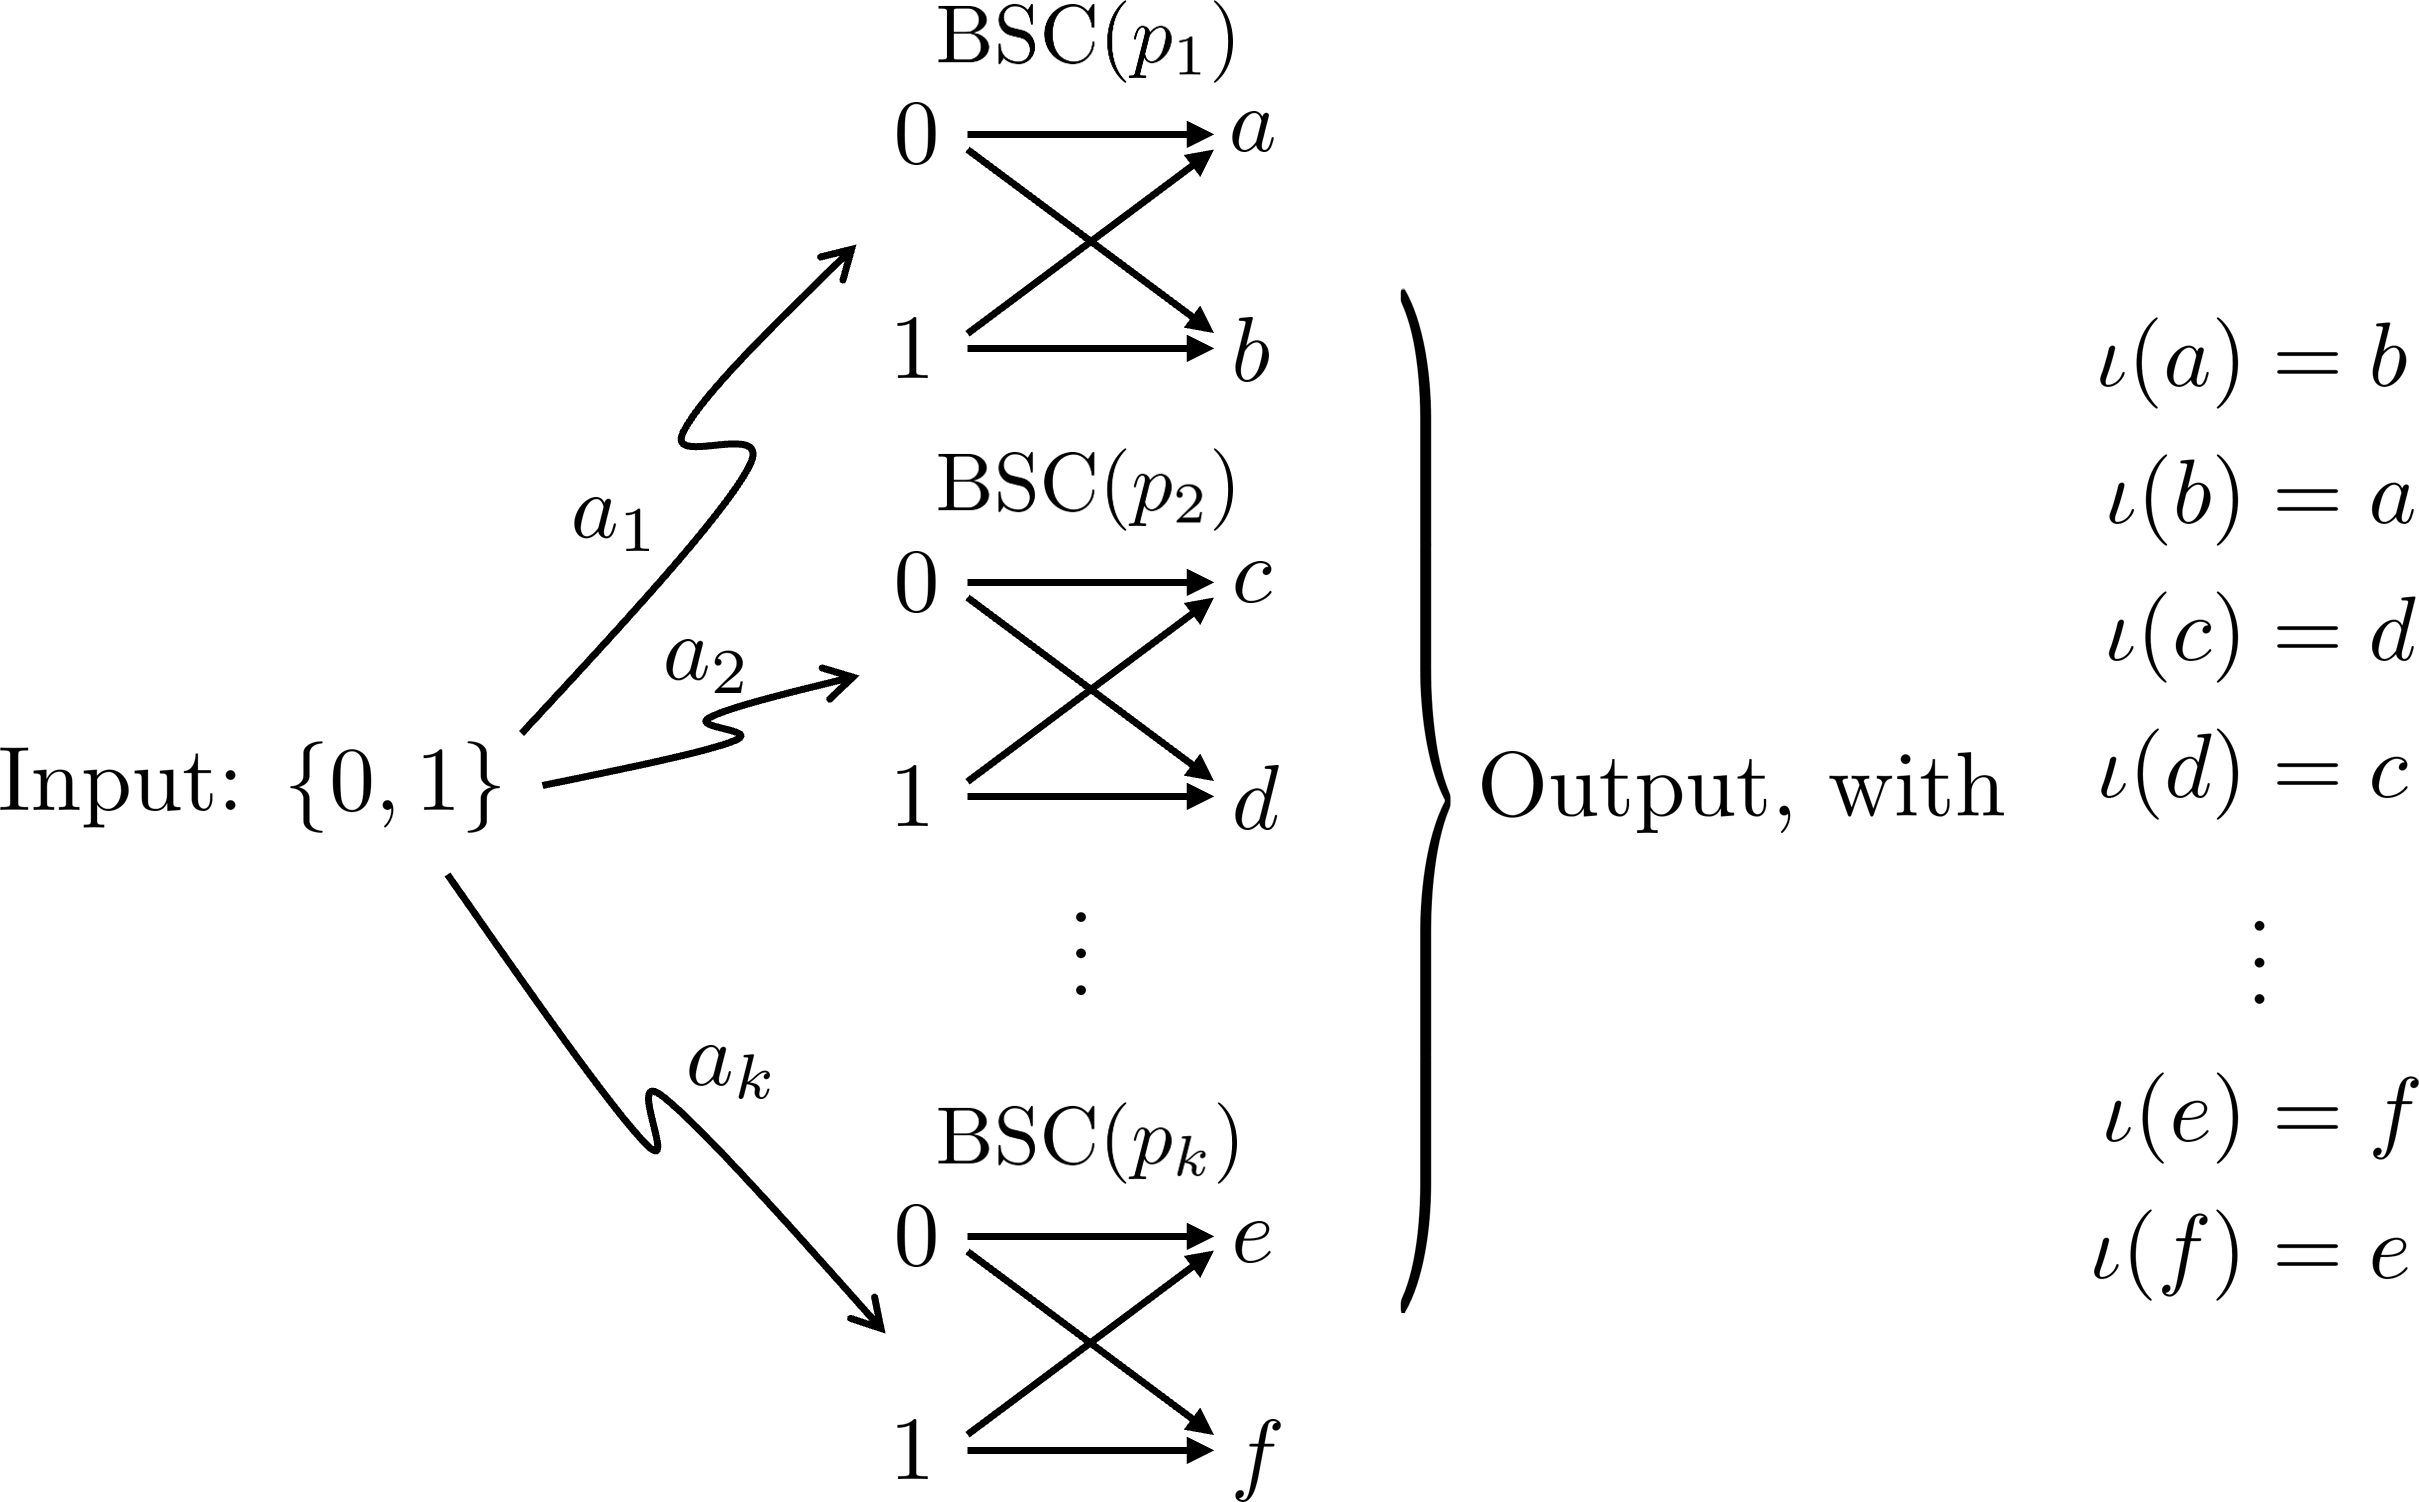
\includegraphics[width=0.7\linewidth]{figures/w3_construct_BMSC.png}
    \caption{Illustration of a general BMSC.}
\end{figure}
By probabilistically assigning a channel $\mathrm{BSC}(p_i)$ with probability $a_i$, we can create seemingly any possible BMSC using BSCs. Note that the involution relations are needed.


In general, we have the following theorem.
\begin{theorem}[BMSC as a Compound of BSCs]
    Given $0<p_1,\ldots,p_k\le\frac{1}{2}$ and $0<a_1,\ldots,a_k<1$ satisfying $a_1+\cdots+a_k=1$, the compound channel
    \begin{equation}
        \sum_{i=1}^k a_i\cdot\mathrm{BSC}(p_i)
    \end{equation}
    is a BMSC. Similarly, any BMSC is equivalent to a decomposition $\sum_{i=1}^k a_i\cdot\mathrm{BSC}(p_i)$.
\end{theorem}
The convex combination of channels corresponds to a probabilistic mixture of the channels.

\begin{remark}
    The decomposition of a BMSC into BSCs holds true even for continuous channels such as an AWGN, where we can replace the summation by an integral:
    \begin{equation*}
        \mathrm{AWGN}(\sigma) = \int A_\sigma(p)\; \mathrm{BSC}(p)\;\dd p.
    \end{equation*}
\end{remark}

For a more general construction and detailed descriptions on BMSC, please refer to the book ``Modern Coding Theory'' \cite{Modern_Coding_Theory} and the paper ``Channel Polarization through the Lens of Blackwell Measures'' \cite{Blackwell_Measure}.


\subsection{The $+$ and $-$ Sub-Channels}
From the above, we know that we can obtain analytical results of any BMSC by analyzing BSCs. In this subsection, we aim to understand the meaning to $\mathrm{BSC}(p)^+$, $\sum a_i\,\mathrm{BSC}(p_i)^+$, $\mathrm{BSC}(p)^-$, and $\sum a_i\,\mathrm{BSC}(p_i)^-$. The paper ``Channel Polarization through the Lens of Blackwell Measures'' \cite{Blackwell_Measure} again provided a detailed and expansive discussion of the following topic.

The most general language that we can use the discussion over the \textit{parallel} and \textit{serial combination} of BSCs, which are denoted by $\mathrm{BSC}(p) \ostar \mathrm{BSC}(q)$ and $\mathrm{BSC}(p) \boxstar \mathrm{BSC}(q)$, respectively. \\

\paragraph{Parallel Combination:}
The parallel combination channel $\mathrm{BSC}(p)\ostar\mathrm{BSC}(q)$ describes what we know about $x\in\{0,1\}$ given the outputs $\mathrm{BSC}(p)(x)$ and $\mathrm{BSC}(q)(x)$. The diagram of the channel is as shown below:
\begin{figure}[H]
    \centering
    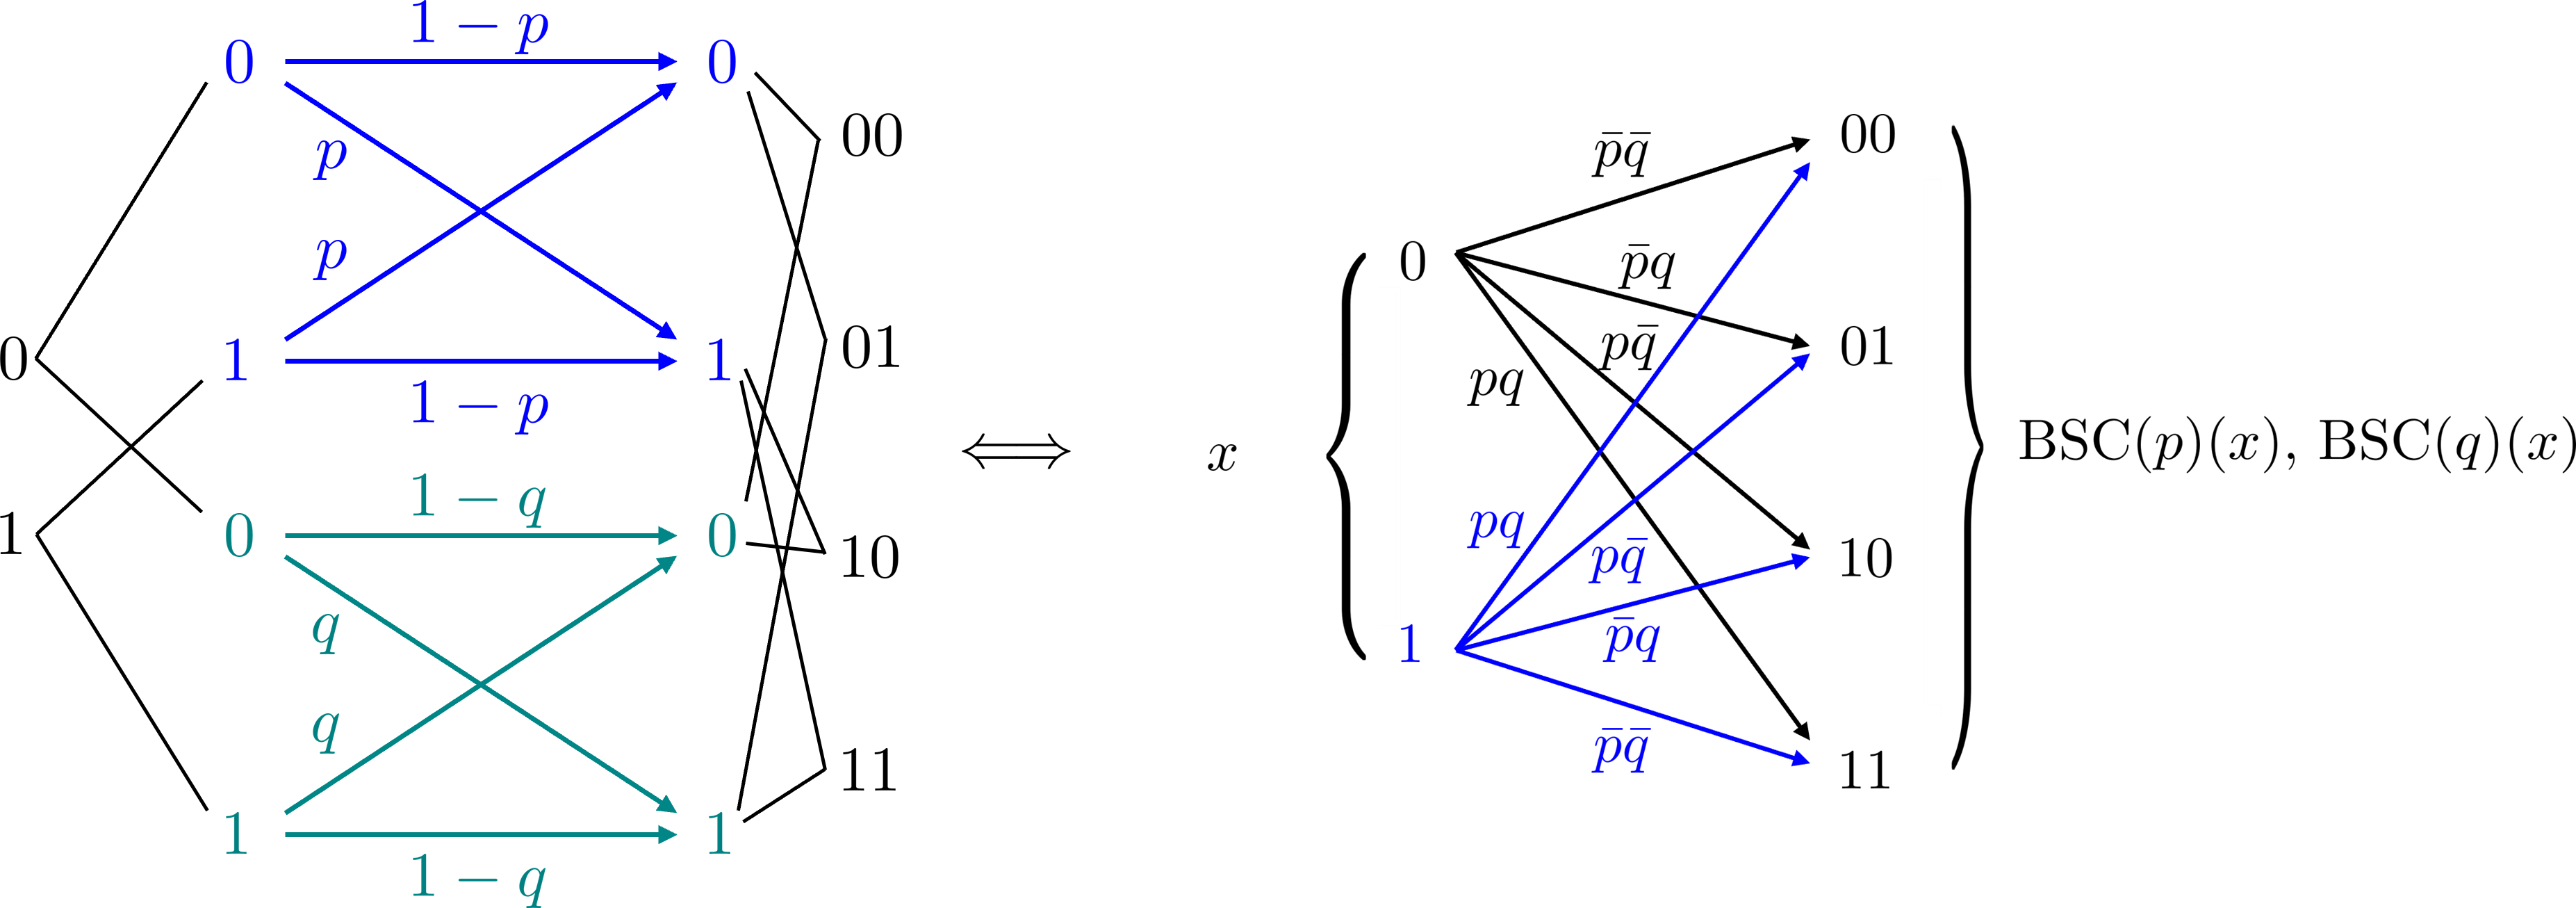
\includegraphics[width=1\linewidth]{figures/w3_parallel_combination.png}
    \caption{Parallel combination of $\textcolor{blue}{\mathrm{BSC}(p)}\ostar\textcolor{teal}{\mathrm{BSC}(q)}$. An input is sent through two parallel channels, with the output compared in parallel to obtain information about the input.}
\end{figure}
By introducing the notation $\bar{x}=1-x$, we have the involution $\iota(x)=\bar{x}$. Furthermore, by an abuse of notation, we also have $\bar{p}=1-p$ and $\bar{q}=1-q$. For an input of $x$, we have the outputs
\begin{align*}
    \begin{cases}
        xx &\text{w.p. }\bar{p}\bar{q},\\
        \bar{x}\bar{x} &\text{w.p. }pq,\\
        x\bar{x} &\text{w.p. }\bar{p}{q},\\
        \bar{x}x &\text{w.p. }{p}\bar{q}.
    \end{cases}
\end{align*}
Henceforth, by considering the involute pairs of $(xx,\bar{x}\bar{x})$ and $(\bar{x}x,x\bar{x})$ as the individual BSC components (since $\iota(xx)=\bar{x}\bar{x}$ and $\iota(\bar{x}x)=x\bar{x}$), we can view the combined channel as
\begin{equation}
    \mathrm{BSC}(p) \ostar \mathrm{BSC}(q) = (pq+\bar{p}\bar{q}) \cdot \mathrm{BSC}\left(\frac{pq}{pq+\bar{p}\bar{q}}\right) + (p\bar{q}+\bar{p}q) \cdot \mathrm{BSC}\left(\frac{p\bar{q}}{p\bar{q}+\bar{p}q}\right).
\end{equation}
The result can be further extended by linearity to
\begin{equation}
    \left(\sum_i a_i \cdot \mathrm{BSC}(p_i)\right) \ostar \left(\sum_i b_i \cdot \mathrm{BSC}(q_i)\right) = \sum_{i,j} a_ib_j \cdot\mathrm{BSC}(p_i)\ostar\mathrm{BSC}(q_j).
\end{equation}


\paragraph{Serial Combination:} The serial combination channel $\mathrm{BSC}(p)\boxstar\mathrm{BSC}(q)$ describes what we know about $x+y$ (mod 2 addition) given the outputs $\mathrm{BSC}(p)(x)$ and $\mathrm{BSC}(q)(y)$. The diagram of the channel is as shown below:
\begin{figure}[H]
    \centering
    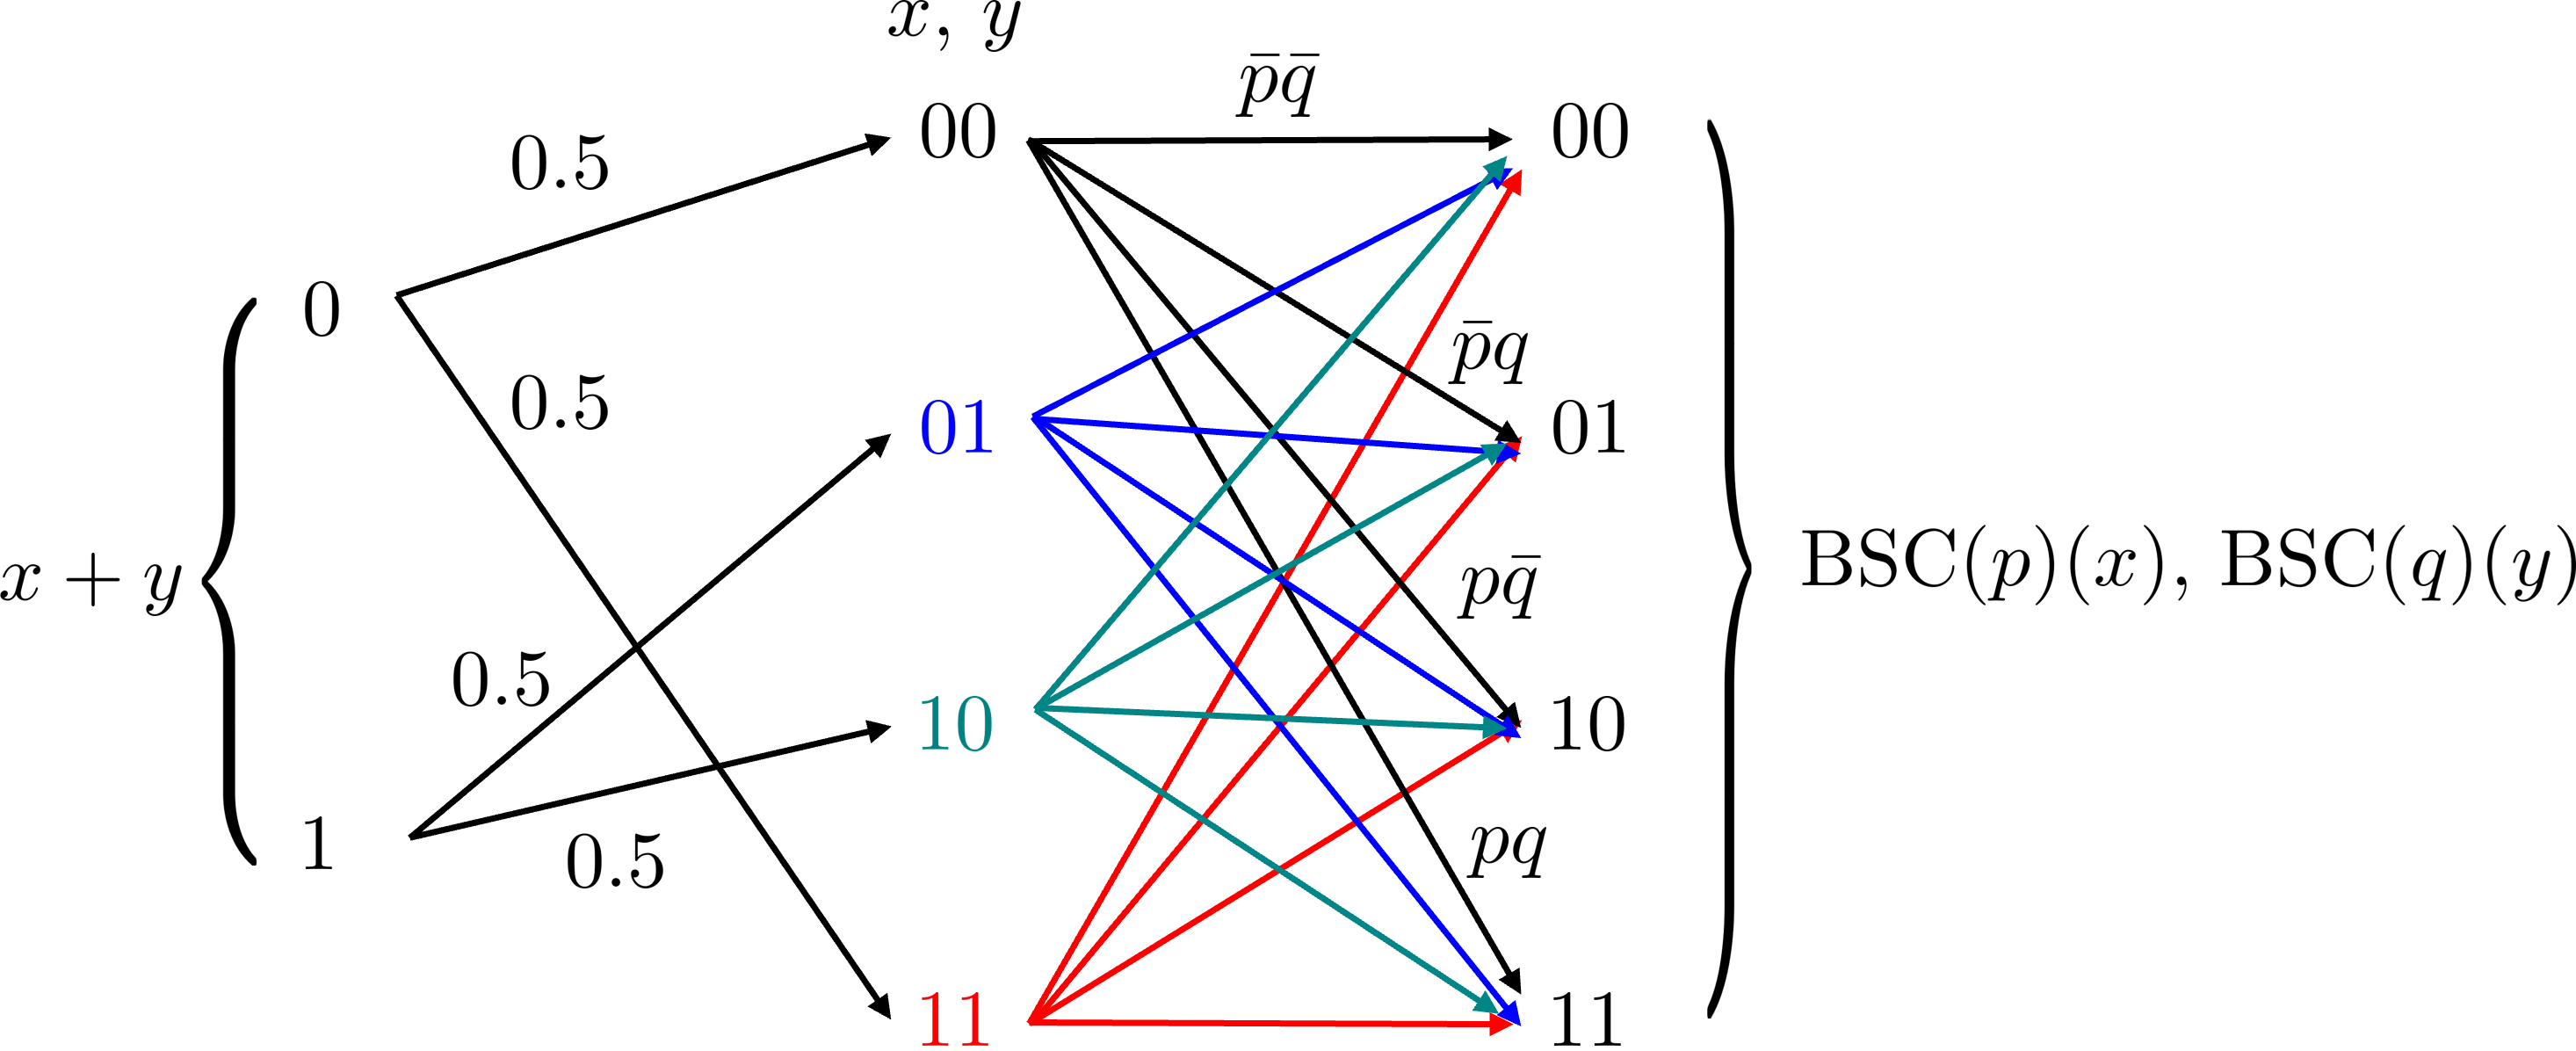
\includegraphics[width=0.8\linewidth]{figures/w3_serial_combination.png}
    \caption{Serial combination of channels. An input is sent through two channels with the output summed together. For the two channels both being BSC, the total effect is equivalent to serial combining the two channels where the output of the first becomes the input of the second.}
    \label{fig:w3_serial}
\end{figure}
The combined channel law is
\begin{align*}
    W(00\vert0) = W(11\vert0) = W(01\vert1) = W(10\vert1) &= \frac{1}{2}(\bar{p}\bar{q}+pq),\\
    W(01\vert0) = W(10\vert0) = W(00\vert1) = W(11\vert1) &= \frac{1}{2}(\bar{p}q+p\bar{q}).
\end{align*}
By considering the super-symbols of involute pairs $A=(00,11)$ and $B=(01,10)$ since the symbols in each super-symbol provides the same information over what $x+y$ is, one can check that the above channel is equivalent to the channel below.
\begin{figure}[H]
    \centering
    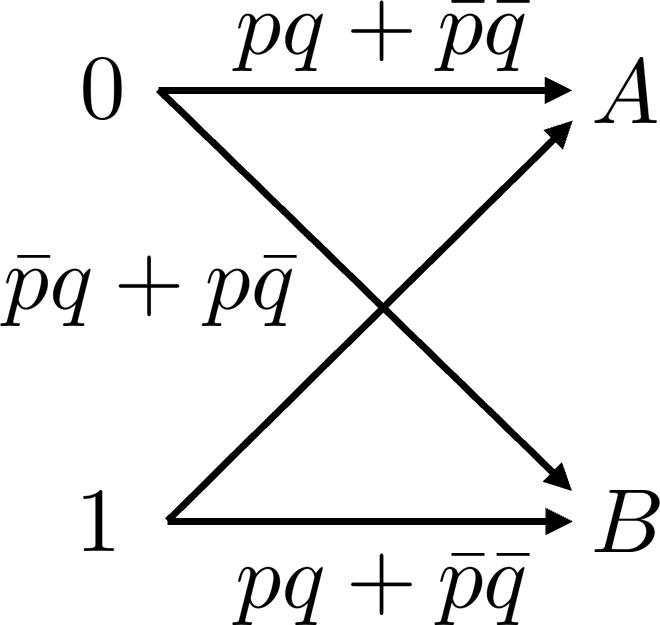
\includegraphics[width=0.2\linewidth]{figures/w3_serial_combination_reduced.png}
    \caption{The serial combination of BSC's is still a BSC.}
\end{figure}
Henceforth, we can view the combined channel as
\begin{equation}
    \mathrm{BSC}(p)\boxstar\mathrm{BSC}(q) = \mathrm{BSC}(pq+\bar{p}\bar{q}).
\end{equation}
The result can be further extended by linearity to
\begin{equation}
    \left(\sum_i a_i \cdot \mathrm{BSC}(p_i)\right) \boxstar \left(\sum_i b_i \cdot \mathrm{BSC}(q_i)\right) = \sum_{i,j} a_ib_j \cdot\mathrm{BSC}(p_i)\boxstar\mathrm{BSC}(q_j).
\end{equation}

\begin{theorem}[Parallel and Serial Combination of BSC]
    For probabilities $p$ and $q$, we have
    \begin{align}
        \mathrm{BSC}(p) \ostar \mathrm{BSC}(q) &= (pq+\bar{p}\bar{q}) \cdot \mathrm{BSC}\left(\frac{pq}{pq+\bar{p}\bar{q}}\right) + (p\bar{q}+\bar{p}q) \cdot \mathrm{BSC}\left(\frac{p\bar{q}}{p\bar{q}+\bar{p}q}\right) \label{w3:BSC_parallel}\\
        \mathrm{BSC}(p)\boxstar\mathrm{BSC}(q) &= \mathrm{BSC}(pq+\bar{p}\bar{q}). \label{w3:BSC_serial}
    \end{align}
\end{theorem}

Note that we can clarify the terms mentioned at the start of this subsection by the following theorem:
\begin{theorem}[The $+$ and $-$ Sub-Channels for BSC]
    For sub-channels of a BSC, we have
    \begin{align}
        \mathrm{BSC}(p)^+ &= \mathrm{BSC}(p)\ostar\mathrm{BSC}(p),\\
        \mathrm{BSC}(p)^- &= \mathrm{BSC}(p)\boxstar\mathrm{BSC}(p).
    \end{align}
\end{theorem}

Lastly, note that for the special case where we are only considering the serial combination of BSCs, and with super-symbols in mind, \autoref{fig:w3_serial} can be transformed into \autoref{fig:w3_serial_BSC}.
\begin{figure}[H]
    \centering
    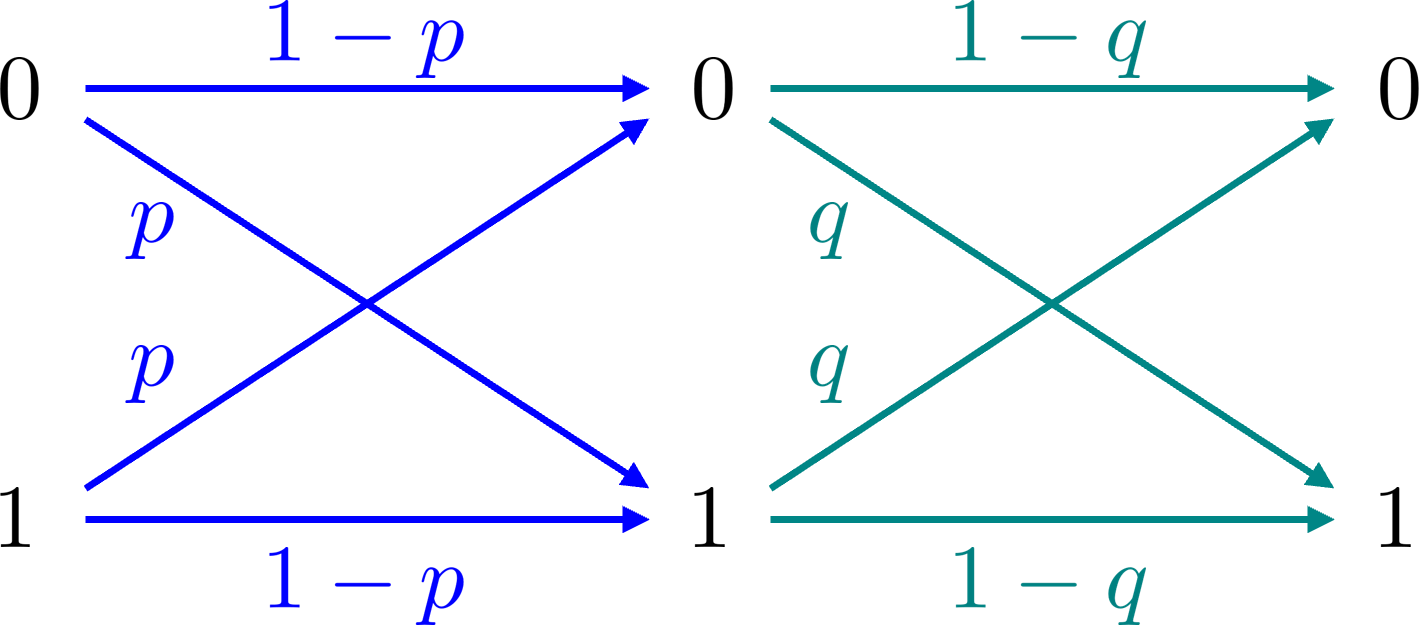
\includegraphics[width=0.5\linewidth]{figures/w3_serial_BSC.png}
    \caption{Serial combination of $\textcolor{blue}{\mathrm{BSC}(p)}\boxstar\textcolor{teal}{BSC}(q)$.}
    \label{fig:w3_serial_BSC}
\end{figure}


By the referenced provided (using the tools derived from the \textit{Blackwell measures}), we have the following general result.
\begin{theorem}[Polar Transform]
    Given two BMSCs $(W_1,\mathcal{Y}_1)$ and $(W_2,\mathcal{Y}_2)$, the \textit{polar transform} maps them into another pair of BMSCs $W_1\ostar W_2$ and $W_1\boxstar W_2$ defined as
    \begin{align}
        (W_1\ostar W_2)(y_1,y_2,u\vert x) &\defeq \frac{1}{2} W_1(y_1\vert x+u) W_2(y_2\vert x), \label{eq:w3_parallel}\\
        (W_1\boxstar W_2)(y_1,y_2\vert x) &\defeq \frac{1}{2} \sum_{u\in\{0,1\}} W_1(y_1\vert x+u) W_2(y_2\vert u) \label{eq:w3_serial}
    \end{align}
    for all $y_1\in\mathcal{Y}_1$, $y_2\in\mathcal{Y}_2$, and $x,u\in\{0,1\}$. The former sub-channel is an improved channel, while the latter is a weaker channel. Especially when $W_1=W_2=W$, we have
    \begin{equation}
        W^+ = W\ostar W \text{ and } W^- = W\boxstar W,
    \end{equation}
    where the equality, if written rigorously, should be an \textit{equivalence} by the \textit{Blackwell measure}.
\end{theorem}
It can be readily seen that under the polar coding scheme: by setting $u_1=u$ and $u_2=x$, with $u$ uniformly distributed, \autoref{eq:w3_parallel} represents the probability of inputting $(u,x)$ and having a channel output of $(y_1,y_2)$ -- if $W_1=W_2=W$, and we group certain symbols into a super-symbol by considering how the polar decoder decodes, this is indeed the channel $W^+$.

Similarly, by setting $u_1=x$ and $u_2=u$, with $u$ uniformly distributed, \autoref{eq:w3_serial} represents the probability of inputting $(x,u)$ and having a channel output of $(y_1,y_2)$ -- if $W_1=W_2=W$, and we group certain symbols into a super-symbol by considering how the polar decoder decodes, this is indeed the channel $W^-$.

% We provide here an alternate proof of this general theorem here, which doesn't require the knowledge of Blackwell measures.
% \begin{proof}
%     Let us consider the two cases separately.
% \begin{enumerate}
%     \item $W_1\ostar W_2$: Under the terminologies of polar code, consider calling $u_1=u$, and $u_2=x$, let us consider the transition probability from $x$ to $(y_1,y_2,u)$ with a uniform prior on $u$. It should be immediate that one arrives at right hand side of \autoref{eq:w3_parallel}. This definition coincide with that of \autoref{eq:w3_parallel_BSC}. For $W_1=W_2$, this is also exactly how we define $W^+$. Hence the equality.

%     \item $W_1\boxstar W_2$: Under the terminologies of polar code, consider calling $u_1=x$, and $u_2=u$, let us consider the transition probability from $x$ to $(y_1,y_2)$ with a uniform prior on $u$. It should be immediate that one arrives at right hand side of \autoref{eq:w3_serial}. This definition coincide with that of \autoref{eq:w3_serial_BSC} in which we consider the transition from $x$ to $y_1+y_2$ if $\mathcal{Y}_1=\mathcal{Y}_2=\{0,1\}$. For $W_1=W_2$, this is also exactly how we define $W^-$. Hence the equality.
% \end{enumerate}
% \end{proof}

Let us demonstrate the theorem above by the following two examples:
\begin{example}
    It can be readily checked that the following equation holds:
    \begin{equation}
        \mathrm{BEC}(x) = \bar{x}\cdot\mathrm{BSC}(1) + x\cdot\mathrm{BSC}(1/2).
    \end{equation}
    Henceforth, we have the two sub-channels calculated to be
    \begin{align*}
        \mathrm{BEC}(x)^+ &= \left(\bar{x} \cdot \mathrm{BSC}(1) + x \cdot \mathrm{BSC}(1/2)\right) \ostar \left(\bar{x} \cdot \mathrm{BSC}(1) + x \cdot \mathrm{BSC}(1/2)\right) \\
        &= \bar{x}^2 \cdot \mathrm{BSC}(1)^+ + x^2 \cdot \mathrm{BSC}(1/2)^+ +2\bar{x}x \cdot \mathrm{BSC}(1)\ostar\mathrm{BSC}(1/2) \\
        &= (1-2x+x^2) \cdot \mathrm{BSC}(1) + x^2 \cdot \mathrm{BSC}(1/2) + (2x-2x^2) \cdot \mathrm{BSC}(1) \\
        &= (1-x^2) \cdot \mathrm{BSC}(1) + x^2 \cdot \mathrm{BSC}(1/2) \\
        &= \mathrm{BEC}(x^2),
    \end{align*}
    \begin{align*}
        \mathrm{BEC}(x)^- &= \left(\bar{x} \cdot \mathrm{BSC}(1) + x \cdot \mathrm{BSC}(1/2)\right) \boxstar \left(\bar{x} \cdot \mathrm{BSC}(1) + x \cdot \mathrm{BSC}(1/2)\right) \\
        &= \bar{x}^2 \cdot \mathrm{BSC}(1)^- + x^2 \cdot \mathrm{BSC}(1/2)^- + 2\bar{x}x \cdot \mathrm{BSC}(1)\boxstar\mathrm{BSC}(1/2) \\
        &= (1-2x+x^2) \cdot \mathrm{BSC}(1) + x^2 \cdot \mathrm{BSC}(1/2) + (2x-2x^2) \cdot \mathrm{BSC}(1/2) \\
        &= (1-2x+x^2) \cdot \mathrm{BSC}(1) + (2x-x^2) \cdot \mathrm{BSC}(1/2)\\
        &= \mathrm{BEC}(2x-x^2).
    \end{align*}
    Thus, we have proven the sub-channel laws of polar code on BEC observed in the first chapter, where $\ostar$ results in a better sub-channel, and $\boxstar$ results in a worse sub-channel.
\end{example}
\begin{example}
    The sub-channels to BEC can also be directly calculated from the polar transformation. Note that $W_1=W_2 = \mathrm{BEC}(x)$ and $\mathcal{Y}_1=\mathcal{Y}_2=\{0,1,\mathcal{E}\}$. Hence, by abbreviating $W\ostar W$ as $W_p$, we have for parallel combination
    \begin{align*}
        \frac{1}{2}\bar{x}^2 &= W_p(0,0,0\vert0) = W_p(1,1,0\vert1) = W_p(1,0,1\vert0) = W_p(0,1,1\vert1), \\
        \frac{1}{2}\bar{x}x &= W_p(\mathcal{E},0,0\vert0) = W_p(\mathcal{E},1,0\vert1) = W_p(\mathcal{E},0,1\vert0) = W_p(\mathcal{E},1,1\vert1) \\
        &= W_p(0,\mathcal{E},0\vert0) = W_p(1,\mathcal{E},0\vert1) = W_p(1,\mathcal{E},1\vert0) = W_p(0,\mathcal{E},1\vert1), \\
        \frac{1}{2}x^2 &= W_p(\mathcal{E},\mathcal{E},0\vert0) = W_p(\mathcal{E},\mathcal{E},0\vert1) = W_p(\mathcal{E},\mathcal{E},1\vert0) = W_p(\mathcal{E},\mathcal{E},1\vert1),
    \end{align*}
    all the other cases have a value of 0. Consider the following disjoint sets of possible outputs,
    \begin{align*}
        \mathcal{S}_0 &= \{(0,0,0),(1,0,1),(\mathcal{E},0,0),(0,\mathcal{E},0),(\mathcal{E},0,1),(1,\mathcal{E},1)\}, \\
        \mathcal{S}_1 &= \{(1,1,0),(0,1,1),(\mathcal{E},1,0),(1,\mathcal{E},0),(\mathcal{E},1,1),(0,\mathcal{E},1)\}, \\
        \mathcal{S}_\mathcal{E} &= \{(\mathcal{E},\mathcal{E},0),(\mathcal{E},\mathcal{E},1)\},
    \end{align*}
    they can be viewed as super-symbols, where the polar decoder will decode $\mathcal{S}_y$ into $y$. Then we can calculate the probability of each set happening:
    \begin{align*}
        1-x^2 &= \mathrm{Pr}\{\mathcal{S}_0\vert0\} = \mathrm{Pr}\{\mathcal{S}_1\vert1\},\\
        0 &= \mathrm{Pr}\{\mathcal{S}_1\vert0\} = \mathrm{Pr}\{\mathcal{S}_0\vert1\},\\
        x^2 &= \mathrm{Pr}\{\mathcal{S}_\mathcal{E}\vert0\} = \mathrm{Pr}\{\mathcal{S}_\mathcal{E}\vert1\}.
    \end{align*}
    Hence, we have that $\mathrm{BEC}(x)^+ = \mathrm{BEC}(x)\ostar\mathrm{BEC}(x) \equiv \mathrm{BEC}(x^2)$.

    Next, let us analyze the serial combination. By abbreviating $W\boxstar W$ as $W_s$, we have
    \begin{align*}
        \frac{1}{2}\bar{x}^2 &= W_s(0,0\vert0) = W_s(1,1\vert0) = W_s(0,1\vert1) = W_s(1,0\vert1), \\
        \frac{1}{2}\bar{x}x &= W_s(\mathcal{E},0\vert0) = W_s(\mathcal{E},1\vert0) = W_s(\mathcal{E},1\vert1) = W_s(\mathcal{E},0\vert1) \\
        &= W_s(0,\mathcal{E}\vert0) = W_s(1,\mathcal{E}\vert0) = W_s(0,\mathcal{E}\vert1) = W_s(1,\mathcal{E}\vert1), \\
        x^2 &= W_s(\mathcal{E},\mathcal{E}\vert0) = W_s(\mathcal{E},\mathcal{E}\vert1).
    \end{align*}
    all the other cases have a value of 0. Consider the following disjoint sets of possible outputs,
    \begin{align*}
        \mathcal{S}_0 &= \{(0,0),(1,1)\}, \\
        \mathcal{S}_1 &= \{(0,1),(1,0)\}, \\
        \mathcal{S}_\mathcal{E} &= \{(\mathcal{E},0),(\mathcal{E},1),(0,\mathcal{E}),(1,\mathcal{E}),(\mathcal{E},\mathcal{E})\},
    \end{align*}
    they are again viewed as super-symbols, representing the decoding scheme. Then we can calculate the probability of each set happening:
    \begin{align*}
        \bar{x}^2 &= \mathrm{Pr}\{\mathcal{S}_0\vert0\} = \mathrm{Pr}\{\mathcal{S}_1\vert1\},\\
        0 &= \mathrm{Pr}\{\mathcal{S}_1\vert0\} = \mathrm{Pr}\{\mathcal{S}_0\vert1\},\\
        2x-x^2 &= \mathrm{Pr}\{\mathcal{S}_\mathcal{E}\vert0\} = \mathrm{Pr}\{\mathcal{S}_\mathcal{E}\vert1\}.
    \end{align*}
    Hence, we have that $\mathrm{BEC}(x)^- = \mathrm{BEC}(x)\boxstar\mathrm{BEC}(x) \equiv \mathrm{BEC}(2x-x^2)$.
\end{example}

By the tedious work above, we have successfully proven the two roads to be equivalent. It should be noted that the grouping of the super-symbols are achieved by considering the polar decoder, which is a decoding scheme based on maximum likelihood test.

\begin{remark}
    Channels can have arbitrary output alphabets, and need not be integers that can be added. For both serial and parallel combinations, we talked about \textit{aggregating} the output symbols in certain ways (for example, adding the symbols as accounting for parity or creating super-symbols), but these interpretations are actually based on the fact that we treat \textit{symbols posing the same coding challenge as the same}.

    We cal a BMSC channel $W:\{0,1\}\rightarrow\mathcal{Y}_W$ a \textit{symbol aggregation} of another BMSC $V:\{0,1\}\rightarrow\mathcal{Y}_V$ if there exists a map $\pi:\mathcal{Y}_V\rightarrow\mathcal{Y}_W$ satisfying
    \begin{equation}\begin{aligned}
        V(y\mid0):V(y\mid1) &= W(\pi(y)\mid0):W(\pi(y)\mid1), \\
        \sum_{v\in\pi^{-1}(y)}V(v\mid0)+V(v\mid1) &= W(y\mid0):W(y\mid1).
    \end{aligned}\end{equation}
\end{remark}

\section{Reed-Muller Code}
\label{sec:RMcode}
\lecture{11 Mar.}

As a closing-off to this chapter, let us look at the Reed-Muller code and its similarities with the polar code. This section is highly related to \autoref{sec:w7_RM_RS}.

Consider the encoding of a 2-layer polar code:
\begin{figure}[H]
    \centering
    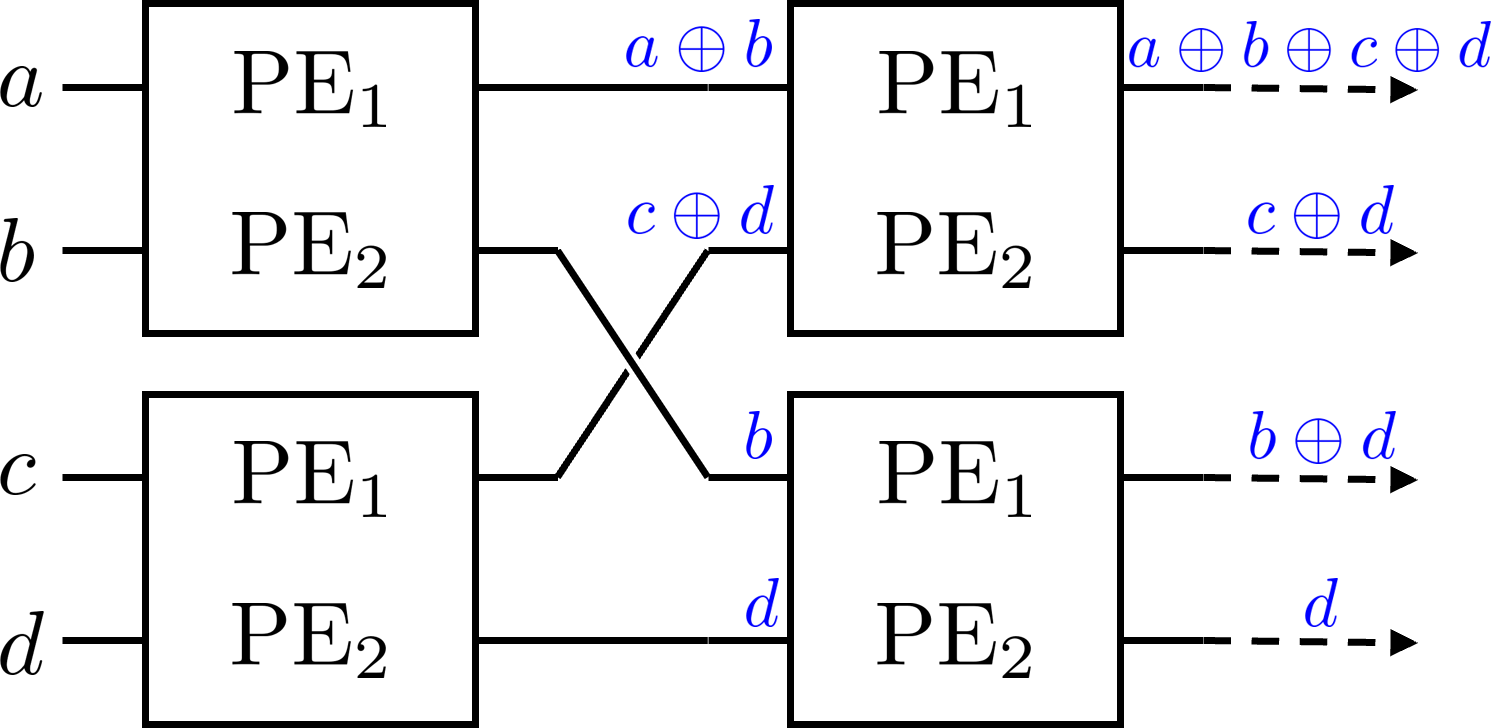
\includegraphics[width=0.4\linewidth]{figures/w4_polar_2layer_enc.png}
    \caption{Codewords of the two-layer polar code.}
\end{figure}
We can rewrite the encoding as a matrix product
\begin{equation}
    \left[\begin{matrix}
        a & c & b & d
    \end{matrix}\right] \left[\begin{matrix}
        1 & 0 & 0 & 0 \\
        1 & 1 & 0 & 0 \\
        1 & 0 & 1 & 0 \\
        1 & 1 & 1 & 1
    \end{matrix}\right] = \left[\begin{matrix}
        a & c & b & d
    \end{matrix}\right] \left[\begin{matrix}
        1 & 0 \\
        1 & 1
    \end{matrix}\right]^{\otimes 2},
\end{equation}
where $\otimes$ is the Kronecker product of matrices.
\begin{definition}[Kronecker Product]
    The Kronecker product of matrices $A= [a_{ij}]$, $B$ is
    \begin{equation}
        A\otimes B = \left[\begin{matrix}
            a_{11} B & a_{12} B & \cdots \\
            a_{21} B & a_{22} B & \cdots \\
            \vdots & \vdots & \ddots
        \end{matrix}\right].
    \end{equation}
    This is also known as the ``tensor product'' of matrices. Note that we also have $A^{\otimes n} = \underbrace{A\otimes \cdots\otimes A}_{n \text{ times}}$.
\end{definition}
In general, under a permutation of the channel orders, we can describe the encoding of an $n$-layer polar code via the matrix
\begin{equation}
    \left[\begin{matrix}
        1 & 0 \\ 1 & 1
    \end{matrix}\right]^{\otimes n},
\end{equation}
this matrix is known as the Ar{\i}kan matrix or the 1011-matrix, which is the \textit{generator matrix} of polar code. By writing out the elements to the Ar{\i}kan matrix explicitly, it beautifully represents the famous fractal \textit{Sierpinski's triangle}. Each row to the Ar{\i}kan's matrix represents a channel $W^s$, where $s\in\{0,1\}^{2^n}$.

Now, how will this help us with the analysis of the code? Recall our scheme for polar code encoding with genie, and compare with the following scheme for Reed-Muller code proposed.
\begin{itemize}
    \item \textbf{Polar Code Encoding:} choose rows of the Ar{\i}kan's matrix with lower $P_e(\mathrm{BEC}(x)^s)$ by applying $f(x)=x^2$ and $g(x)=2x-x^2$ recursively. A partial ordering is created by ordering the error probability.
    \item \textbf{Reed-Muller Code:} choose rows of the Ar{\i}kan's matrix with a lot of $1$'s. Explicitly, choose those with the higher Hamming weights.
\end{itemize}
\begin{example}
    Consider the 3-layer polar code, we have the Ar{\i}kan's matrix with the weights listed as
    \begin{equation*}
        \begin{array}{lc}
            \text{Ar{\i}kan's matrix} & \text{Hamming weight} \\\hline
            1 & 1 \\
            1\;1 & 2 \\
            1\;{\color{lightgray}0}\;1 & 2 \\
            1\;1\;1\;1 & \color{red}4 \\
            1\;{\color{lightgray}0\;0\;0}\;1 & 2 \\
            1\;1\;{\color{lightgray}0\;0}\;1\;1 & \color{red}4 \\
            1\;{\color{lightgray}0}\;1\;{\color{lightgray}0}\;1\;{\color{lightgray}0}\;1 & \color{red}4 \\
            1\;1\;1\;1\;1\;1\;1\;1 & \color{red}8
        \end{array}
    \end{equation*}
    See how those with higher Hamming weights are the ones chosen by the genie! They correspond to those with a lower error probability. Moreover, unlike the analysis of partial ordering over the error probability polynomials. The Hamming weights to $n$-layer polar codes can be easily generalized by doubling the weights to the $(n-1)$-layer polar codes. This is a much simpler ordering scheme when compared to polar code.
\end{example}

The exact amount of rows chosen by the genie to be the good channels under the Reed-Muller code depends on the code rate desired, but the ordering is simply based on the Hamming weights.
\begin{definition}[Reed-Muller Code]
    We define the Reed-Muller code $\mathrm{RM}(r,m)\subseteq\{0,1\}^{2^m}$ as the rows of channels of the Ar{\i}kan's matrix chosen such that their Hamming weights $\ge 2^{m-r}$.
\end{definition}
The higher $r$ is for a given Reed-Muller code $\mathrm{RM}(r,m)$, the higher rate the coding scheme is; on the contrary, for a lower $r$, one pursues a code with high standards.

\begin{remark}
    Some examples to Reed-Muller code listed on Wikipedia are:
    \begin{enumerate}
        \item $\mathrm{RM}(0,m)$: repetition code, 1-dimensional code generate by all-1 vector,
        \item $\mathrm{RM}(m,m)$: the entire space,
        \item $\mathrm{RM}(1,m)$: Hadamard code,
        \item $\mathrm{RM}(m-1,m)$: single-parity-check code,
        \item $\mathrm{RM}(m-2,m)$: extended Hamming code.
    \end{enumerate}
\end{remark}
\chapter{Polar Code in Source Coding}
\section{Source Coding}
\lecture{11 Mar.}

\subsection{Shannon's Source Coding Theorem}
In Shannon's 1948 paper, he introduced source coding as a mean of compression for a source, i.e., a sequence of symbols $X_i$. The information theorist Blahut further defines \textit{compression} as \textit{lossy compression}, and \textit{compaction} as \textit{lossless compression}.

The following information quantity is useful in describing source coding:
\begin{definition}[Entropy]
    For an i.i.d. source $X$ following a probability density function (can be easily extended to the continuous case) $p(x)$, we define its entropy to be
    \begin{equation}
        H(X) = -\sum_{x}p(x)\lg p(x) \text{ bits.}
    \end{equation}
    If $\ln$ is used in place of $\lg$, the units changes from ``bits'' to ``nats''.
\end{definition}
\begin{theorem}[Shannon's Source Coding Theorem]
    Given an i.i.d. source $X_1$, $X_2$, $\ldots$, a total of $H(X)+\varepsilon$ bits are needed per observation to describe the source.
\end{theorem}
\begin{example}
    Consider the following \textit{Huffman coding}, which is an easier version of Shannon's source coding theorem. Let a random source of nucleobases $X$ be equal to $A$ w.p. $\frac{1}{2}$, $C$ w.p. $\frac{1}{4}$, $G$ w.p. $\frac{1}{8}$, or $T$ w.p. $\frac{1}{8}$. Since $-\lg p(A) = 1$, we should use 1 bit to describe $A$; since $-\lg p(C) = 2$, we should use 2 bits to describe $C$; and similarly, we should use 3 bits to describe both $G$ and $T$. For example, we encode the nucleobases by $A:0$, $C:10$, $G:110$, and $T:111$. If one tries to encode $n$ nucleobases, we have the total expected bits used as
    \begin{equation*}
        \frac{n}{2}\cdot1 + \frac{n}{4}\cdot2 + \frac{n}{8}\cdot 3 + \frac{n}{8}\cdot3 = \frac{7}{4}n \text{ bits} = n\cdot H(X).
    \end{equation*}
\end{example}

Let us define a few more terms:
\begin{definition}[Information Density]
    We define the information density / surprisal of a realization $x$ of the random variable $X$ as
    \begin{equation}
        h(x) = -\lg p(x).
    \end{equation}
    Entropy is equal to the expected surprisal, i.e., $H(X) = \mathbb{E}[h(X)]$.
\end{definition}
\begin{definition}[Asymptotic Equipartition Property, AEP]
    This describes the log version of the law of large number. Notice that
    \begin{equation}
        h(x_1\ldots x_n) = -\lg\left(p(x_1)\cdots p(x_n)\right) = \sum_{i=1}^n -\lg p(x_i) = \sum_{i=1}^n h(x_i).
    \end{equation}
    This is an i.i.d. sum of R.V.s! We can use the concentration inequality:
    \begin{equation*}
        \mathrm{Pr}\left\{\frac{\sum_{i=1}^n h(X_i)}{n} - H(X) \ge \varepsilon\right\} \le \exp(-c\varepsilon^2n).
    \end{equation*}
    The AEP property simply states the concentration of the average of information density converges to the entropy.
\end{definition}
Let us now prove the theorem. We will further use polar code to achieve it. 
\begin{proof}[Proof. (Shannon's Source Coding Theorem, fixed length version)]
    Let us try to encode as many length $n$ strings as possible using only $n\left(H(X)+2\varepsilon\right)$ bits. Let us define a \textit{typical set}
    \begin{equation}
        \mathcal{A}(\varepsilon) \defeq \setdef{x_1\ldots x_n \in \mathcal{X}^n}{h(x_1\ldots x_n) \le n\left(H(X)+\varepsilon\right)}.
    \end{equation}
    For a string $x_1\ldots x_n\in\mathcal{A}(\varepsilon)$, we have
    \begin{equation}
        p(x_1\ldots x_n) \ge 2^{-n\left(H(X)+\varepsilon\right)} \Rightarrow \abs{\mathcal{A}(\varepsilon)} \le 2^{n\left(H(X)+\varepsilon\right)}.
    \end{equation}
    Thus, the set $\mathcal{A}(\varepsilon)$ can be mapped injectively onto bit string of length $n\left(H(X)+\varepsilon\right)$. What about the sequences outside of $\mathcal{A}(\varepsilon)$? Luckily, by the concentration inequality, their total probability of appearing is exponentially small and can be neglected.
\end{proof}
\begin{proof}[Proof. (Shannon's Source Coding Theorem, variable length version)]
    If fix length encoding fails to describe a source, we can use the suboptimal ``literal'' encoding for some strings. An encoding of a string either looks to have around $n H(X)$ bits for those in $\mathcal{A}(\varepsilon)$, or that they are described by $Cn$ bits, where $C$ is a constant. Then the expected value of the code length will be
    \begin{align*}
        \mathbb{E}[\text{length}] = \left(1-\exp(-c\varepsilon^2n)\right) \cdot n\left(H(X)+\varepsilon\right) + \exp(-c\varepsilon^2n)\cdot Cn = n\left(H(X)+2\varepsilon\right).
    \end{align*}
\end{proof}

In fact, most of our modern day coding uses variable length coding, as one can easily check that photos saved in your phone album has varying file size.

\subsection{Arithmetic Encoding}
\begin{example}
    Consider a source $X$ being equal to $A$ w.p. $\frac{2}{3}$, equal to $C$ w.p. $\frac{1}{3}$. Then given a string, for example $ACAACAC$, we can encode it into a binary string by the following procedure:
    \begin{figure}[H]
        \centering
        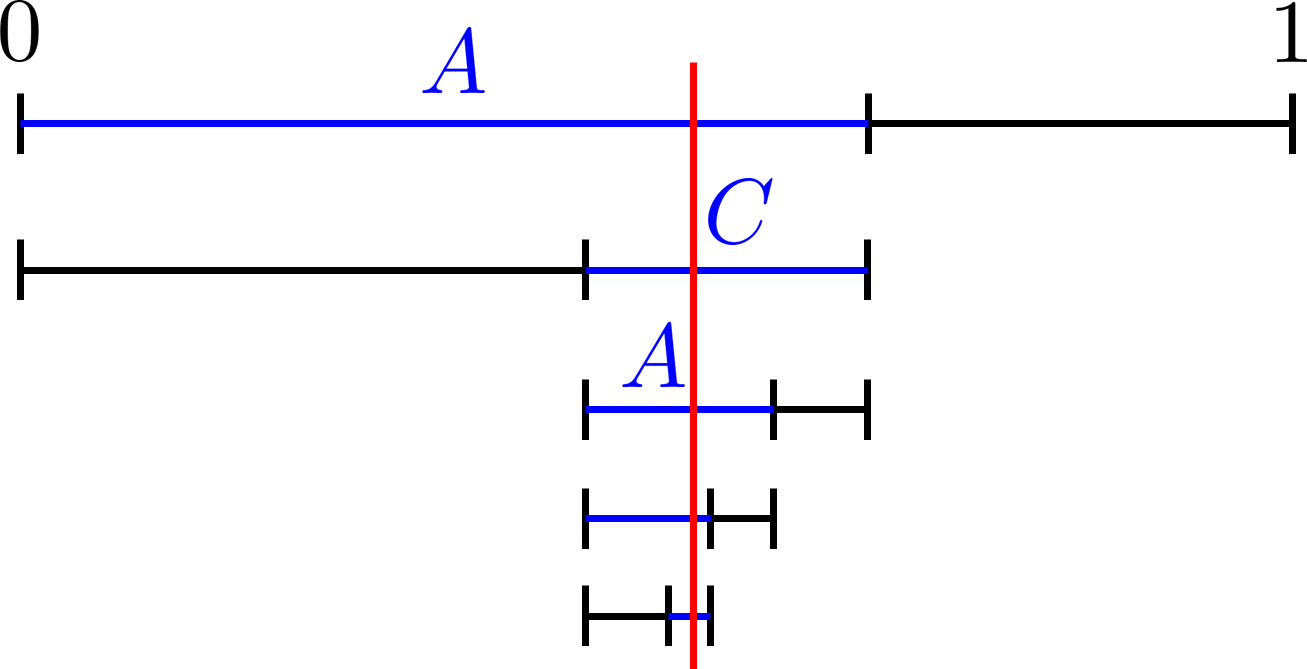
\includegraphics[width=0.5\linewidth]{figures/w4_arithmetic_encoding.png}
        \caption{Illustration of arithmetic encoding.}
    \end{figure}
    By continuing partitioning the interval with respect to the probability one can find a shortest binary string in the last interval and use it to represent the original string of symbols. In our case above, the last interval is $[124/243,44/81]\approx[0.510288,0.543209]$, the shortest bit string within is $0.10001$ in binary. The number of bits needed is approximately
    \begin{align*}
        \lg\frac{1}{\text{smallest interval size}} &= \lg\left(\frac{2}{3}\cdot\frac{1}{3}\cdot\frac{2}{3}\cdot\frac{2}{3}\cdot\frac{1}{3}\cdot\frac{2}{3}\cdot\frac{1}{3}\right)^{-1} \\
        &= -\lg\left(\prod p(x_i)\right)\\
        &\approx -\lg\left.2^{nH(X)}\right|_{n=7} = n H(X)\approx 6.4.
    \end{align*}
\end{example}
Note that arithmetic encoding is in fact capacity-achieving as seen in the example above. However, due to patent reasons, this code is not widely used.

\subsection{Source Coding with Incorrect Code}
Suppose that we have a coding scheme designed specifically for $\mathrm{Ber}(q)$. However, if the true underlying distribution is $\mathrm{Ber}(p)$ where $q\neq p$, what will happen?

Obviously, the compression to the code would not be as good as initially expected. In fact, we can characterize the extra length to the code paid by our ignorance to be
\begin{align*}
    \mathbb{E}_{\mathrm{Ber}(p)}\left[-\lg q(X)\right] - \mathbb{E}_{\mathrm{Ber}(p)}\left[-\lg p(X)\right] &= \left[-p\lg q - (1-p)\lg(1-q)\right] \\
    &\;\;\;\;\;\;- \left[-p\lg p - (1-p)\lg(1-p)\right] \\
    &= p\lg\frac{p}{q} + (1-p)\lg\frac{1-p}{1-q} \\
    &\eqdef D_{\mathrm{KL}}(P\mid\mid Q).
\end{align*}
The term $D_{\mathrm{KL}}$ that we obtained here is another important information theoretical quantity:
\begin{definition}[Kullback-Leibler Divergence, KL Divergence]
    For two distributions $P$ and $Q$, we can define their KL divergence to be
    \begin{equation}
        D_\mathrm{KL}(P\mid\mid Q) \defeq \mathbb{E}_{P}\left[\lg\frac{P}{Q}\right] = \sum p_i \lg\frac{p_i}{q_i}.
    \end{equation}
\end{definition}
It is easy to see that the KL divergence must be greater than or equal to zero. Moreover, given $D_{\mathrm{KL}}(P\mid\mid Q)$, it describes the expected surprise from modeling as $Q$ given the true underlying distribution being $P$.

\subsection{Source Polarization}
For source coding, there are three different methods: Shannon's source coding theorem, arithmetic encoding, and Ar{\i}kan's source polarization. We have talked about the previous two already, let us discuss how the polarization trick we have seen earlier from noisy-channel coding can also be used in source coding. Note that the following trick we introduce has great advantage when we want to apply it to distribution shaping in the future.

In essence, source polarization is equivalent to channel polarization but without looking at the channel outputs. Given two symbols $U_1$, $U_2$ in a field $F$. Then, let us consider a similar scheme as in channel polarization:
\begin{enumerate}
    \item What is the distribution of $X_1\defeq U_1+U_2$?
    \item Given $U_1+U_2$, what is the distribution of $X_2\defeq U_2$?
    \item Do the same polarization recursion: given two copies of $U$ from the same distribution, construct $X_1$ and $X_2$ as $U^+$ and $U^-$. Given two copies of $U^+$, construct $U^{++}$ and $U^{+-}$; given two copies of $U^-$, construct $U^{-+}$ and $U^{--}$. And so on.
\end{enumerate}
One should be able to observe that $H(U^{\pm\pm\ldots})$ polarizes to 0 or $\lg\abs{F}$, which corresponds to a constant random variable or a uniform distribution over $F$, respectively.

The number of $s\in\{+,-\}^n$ such that $H(U^s)\approx 0$ is about $2^n(1-\frac{H(U)}{\lg\abs{F}})$; the number of $s\in\{+,-\}^n$ such that $H(U^s)\approx \lg\abs{F}$ is about $2^n(\frac{H(U)}{\lg\abs{F}})$. By a similar argument using martingale, the quantity going up or down remains balanced so as to have the expectation unchanged. We do not provide a detailed proof here.

The source coding scheme under this setup is: remember those $U^s$ that satisfy $H(U^s) \approx \lg\abs{F}$, i.e., remember those that are random. This scheme is, in fact, capacity-achieving.

Amazingly, polar code can do both source coding and noisy-channel coding as defined by Shannon's 1948 paper.


\subsection{Source Coding with Side Information} \label{sec:slepian_wolf_1}
Given a source that generates a pair of random variables $(X_i,Y_i)$ where $X_i$ is what one tries to remember, and $Y_i$ is the \textit{side information} available at both the encoder and decoder.
\begin{figure}[H]
    \centering
    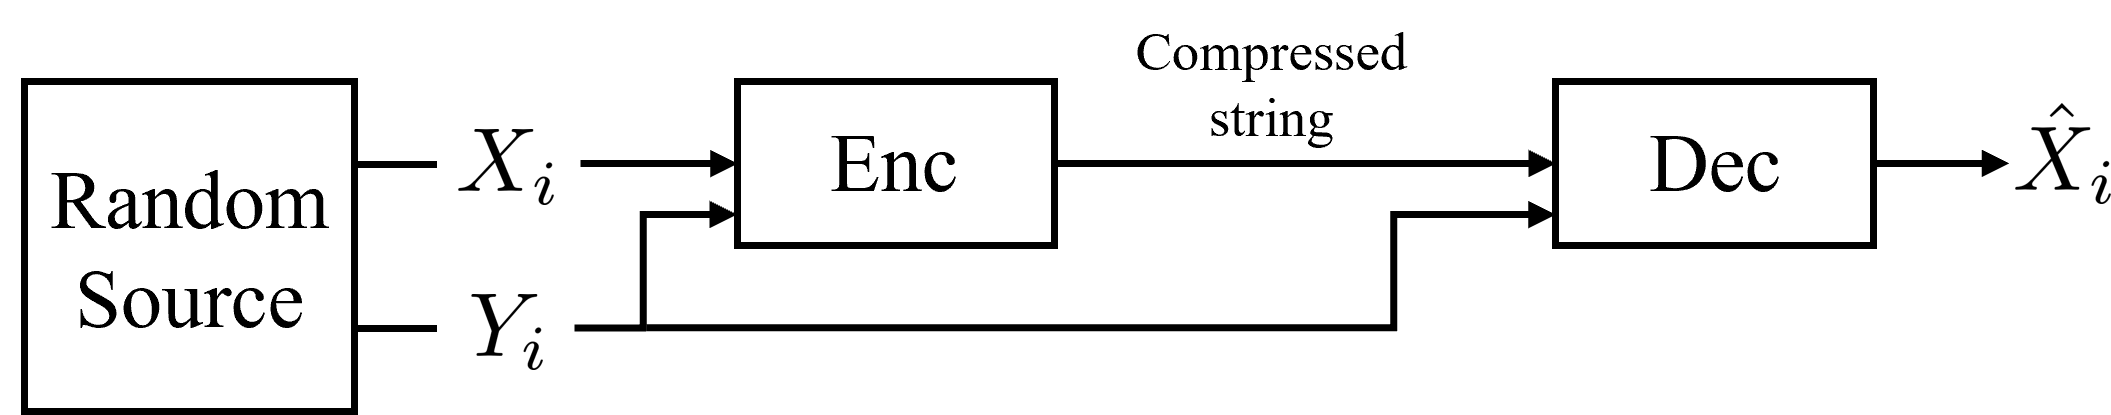
\includegraphics[width=0.8\linewidth]{figures/w4_enc_dec.png}
    \caption{Illustration of source coding with side information.}
\end{figure}
The code rate is the \textit{conditional entropy} $H(X\vert Y) = H(X,Y) = H(Y)$, which satisfies $H(X\vert Y)\le H(X)$. This is the Slepian-Wolf coding, developed after WWII to figure out the amount of information needed to be sent from spy planes with overlapping scanning areas.

The proof to the Slepian-Wolf coding as a valid coding method is similar to that as Shannon's source coding theorem:
\begin{enumerate}
    \item Define conditional information density $h(x_i\vert y_i) = -\lg p(x_i\vert y_i)$.
    \item $h(x_1\ldots x_n\vert y_1\ldots y_n) = $ sum of i.i.d. R.V.s $ = \sum_i h(x_i\vert y_i)$.
    \item $\mathcal{A}(\varepsilon) = \setdef{\text{string}}{h\le n(H(X\vert Y)+\varepsilon)}$. (AEP and typical set)
    \item Find injection between $\mathcal{A}(\varepsilon)$ and strings of length $n(H(X\vert Y)+\varepsilon)$.
    \item Bound error probability by concentration inequality.
\end{enumerate}

Similarly, one can realize the capacity-achieving property using polar code. The proof is also of similar fashion:
\begin{enumerate}
    \item Define polarized random variables $(X\vert Y)^\pm$.
    \item Check for polarization: $H((X\vert Y)^s)=0$ or $\lg\abs{F}$.
    \item Find number of $s$ such that $H$ is high is about $2^n(H(X\vert Y)+\varepsilon)$.
    \item Remember these random variables that are almost uniformly random.
    \item Check for capacity-achieving property.
\end{enumerate}


\section{Channel Parameters}
\lecture{18 Mar.}

Let us define a few channel parameters that will aid our analysis of channels latter on.

We especially consider those that respect the structure of the decomposition of a compound channel into BSCs. Consider an arbitrary BMSC $W=\sum_{i}a_i\mathrm{BSC}(p_i)$, let us define
\begin{definition}[Channel Parameters]
    \begin{itemize}
        \item \textbf{Conditional Entropy}:
        \begin{align}
            &H(W) \defeq \sum_{i}a_i H\left(\mathrm{BSC}(p_i)\right),\\
            &H\left(\mathrm{BSC}(p)\right) \defeq h_b(p) = -p\lg p - \bar{p}\lg\bar{p}.
        \end{align}
        The function $h_b$ is the binary entropy, and $\bar{p}=1-p$. Note that the capacity of a BSC is $C(\mathrm{BSC}(p)) \defeq 1-H(\mathrm{BSC}(p))$.
        \item \textbf{Bhattacharyya Parameter}:
        \begin{align}
            &Z(W) \defeq \sum_{i}a_i Z\left(\mathrm{BSC}(p_i)\right),\\
            &Z\left(\mathrm{BSC}(p)\right) \defeq 2\sqrt{p\bar{p}}.
        \end{align}
        Note that when $p\rightarrow0$ or $1$, $Z\rightarrow0$; when $p\rightarrow\frac{1}{2}$, $Z\rightarrow1$.
        \item \textbf{Total Variation Distance}:
        \begin{align}
            &T(W) \defeq \sum_{i}a_i T\left(\mathrm{BSC}(p_i)\right),\\
            &T\left(\mathrm{BSC}(p)\right) \defeq \abs{1-2p} = \abs{\frac{1}{2}-p} + \abs{\frac{1}{2}-\bar{p}} = \abs{p-\bar{p}}.
        \end{align}
        This parameter is also a symmetric one. Furthermore, it measures how far away our distribution is from the uniform distribution.
        \item \textbf{Bit Error Probability}:
        \begin{align}
            &P_e(W) \defeq \sum_{i}a_i P_e\left(\mathrm{BSC}(p_i)\right),\\
            &P_e\left(\mathrm{BSC}(p)\right) \defeq 2\min\{p,\bar{p}\}.
        \end{align}
        Where does the mysterious 2 come from? Observe the following example for an explanation.
    \end{itemize}
\end{definition}

\begin{example}
    Consider a channel $\mathrm{BEC}(x) = \bar{x}~\mathrm{BSC}(0) + x~\mathrm{BSC}(1/2)$. The error probability actually depends on how we want to decode it. If one simply gives up when seeing an erasure output, the error probability will be $P_e(\mathrm{BSC}(x))=x$. However, if we try really hard and simply guess when receiving an erasure, the error probability will be, under a uniform prior, $P_e(\mathrm{BSC}(x))=x/2$.

    It is of a notational agreement that when considering the channel parameter $P_e$, we let it be characterizing the error probability when we simply give up. Henceforth, we have
    \begin{equation*}
        P_e\left(\mathrm{BEC}(x)\right) = \bar{x}~P_e\left(\mathrm{BSC}(0)\right) + x~P_e\left(\mathrm{BSC}(1/2)\right) = \bar{x}\cdot0 + x\cdot2\cdot\frac{1}{2} = x.
    \end{equation*}
    The benefit of this notational agreement will be the fact that $P_e\left(\mathrm{BSC}(p)\right)\in[0,1]$ for all $p$, and so is their convex combination. This is the same for all other parameters we just introduced, they all lie in the interval $[0,1]$.
\end{example}
These parameters will be shown to be really useful in characterizing how good a channel is. And by converting between different parameters, many of the properties of a channel can be characterized as well.

\begin{figure}[H]
    \centering
    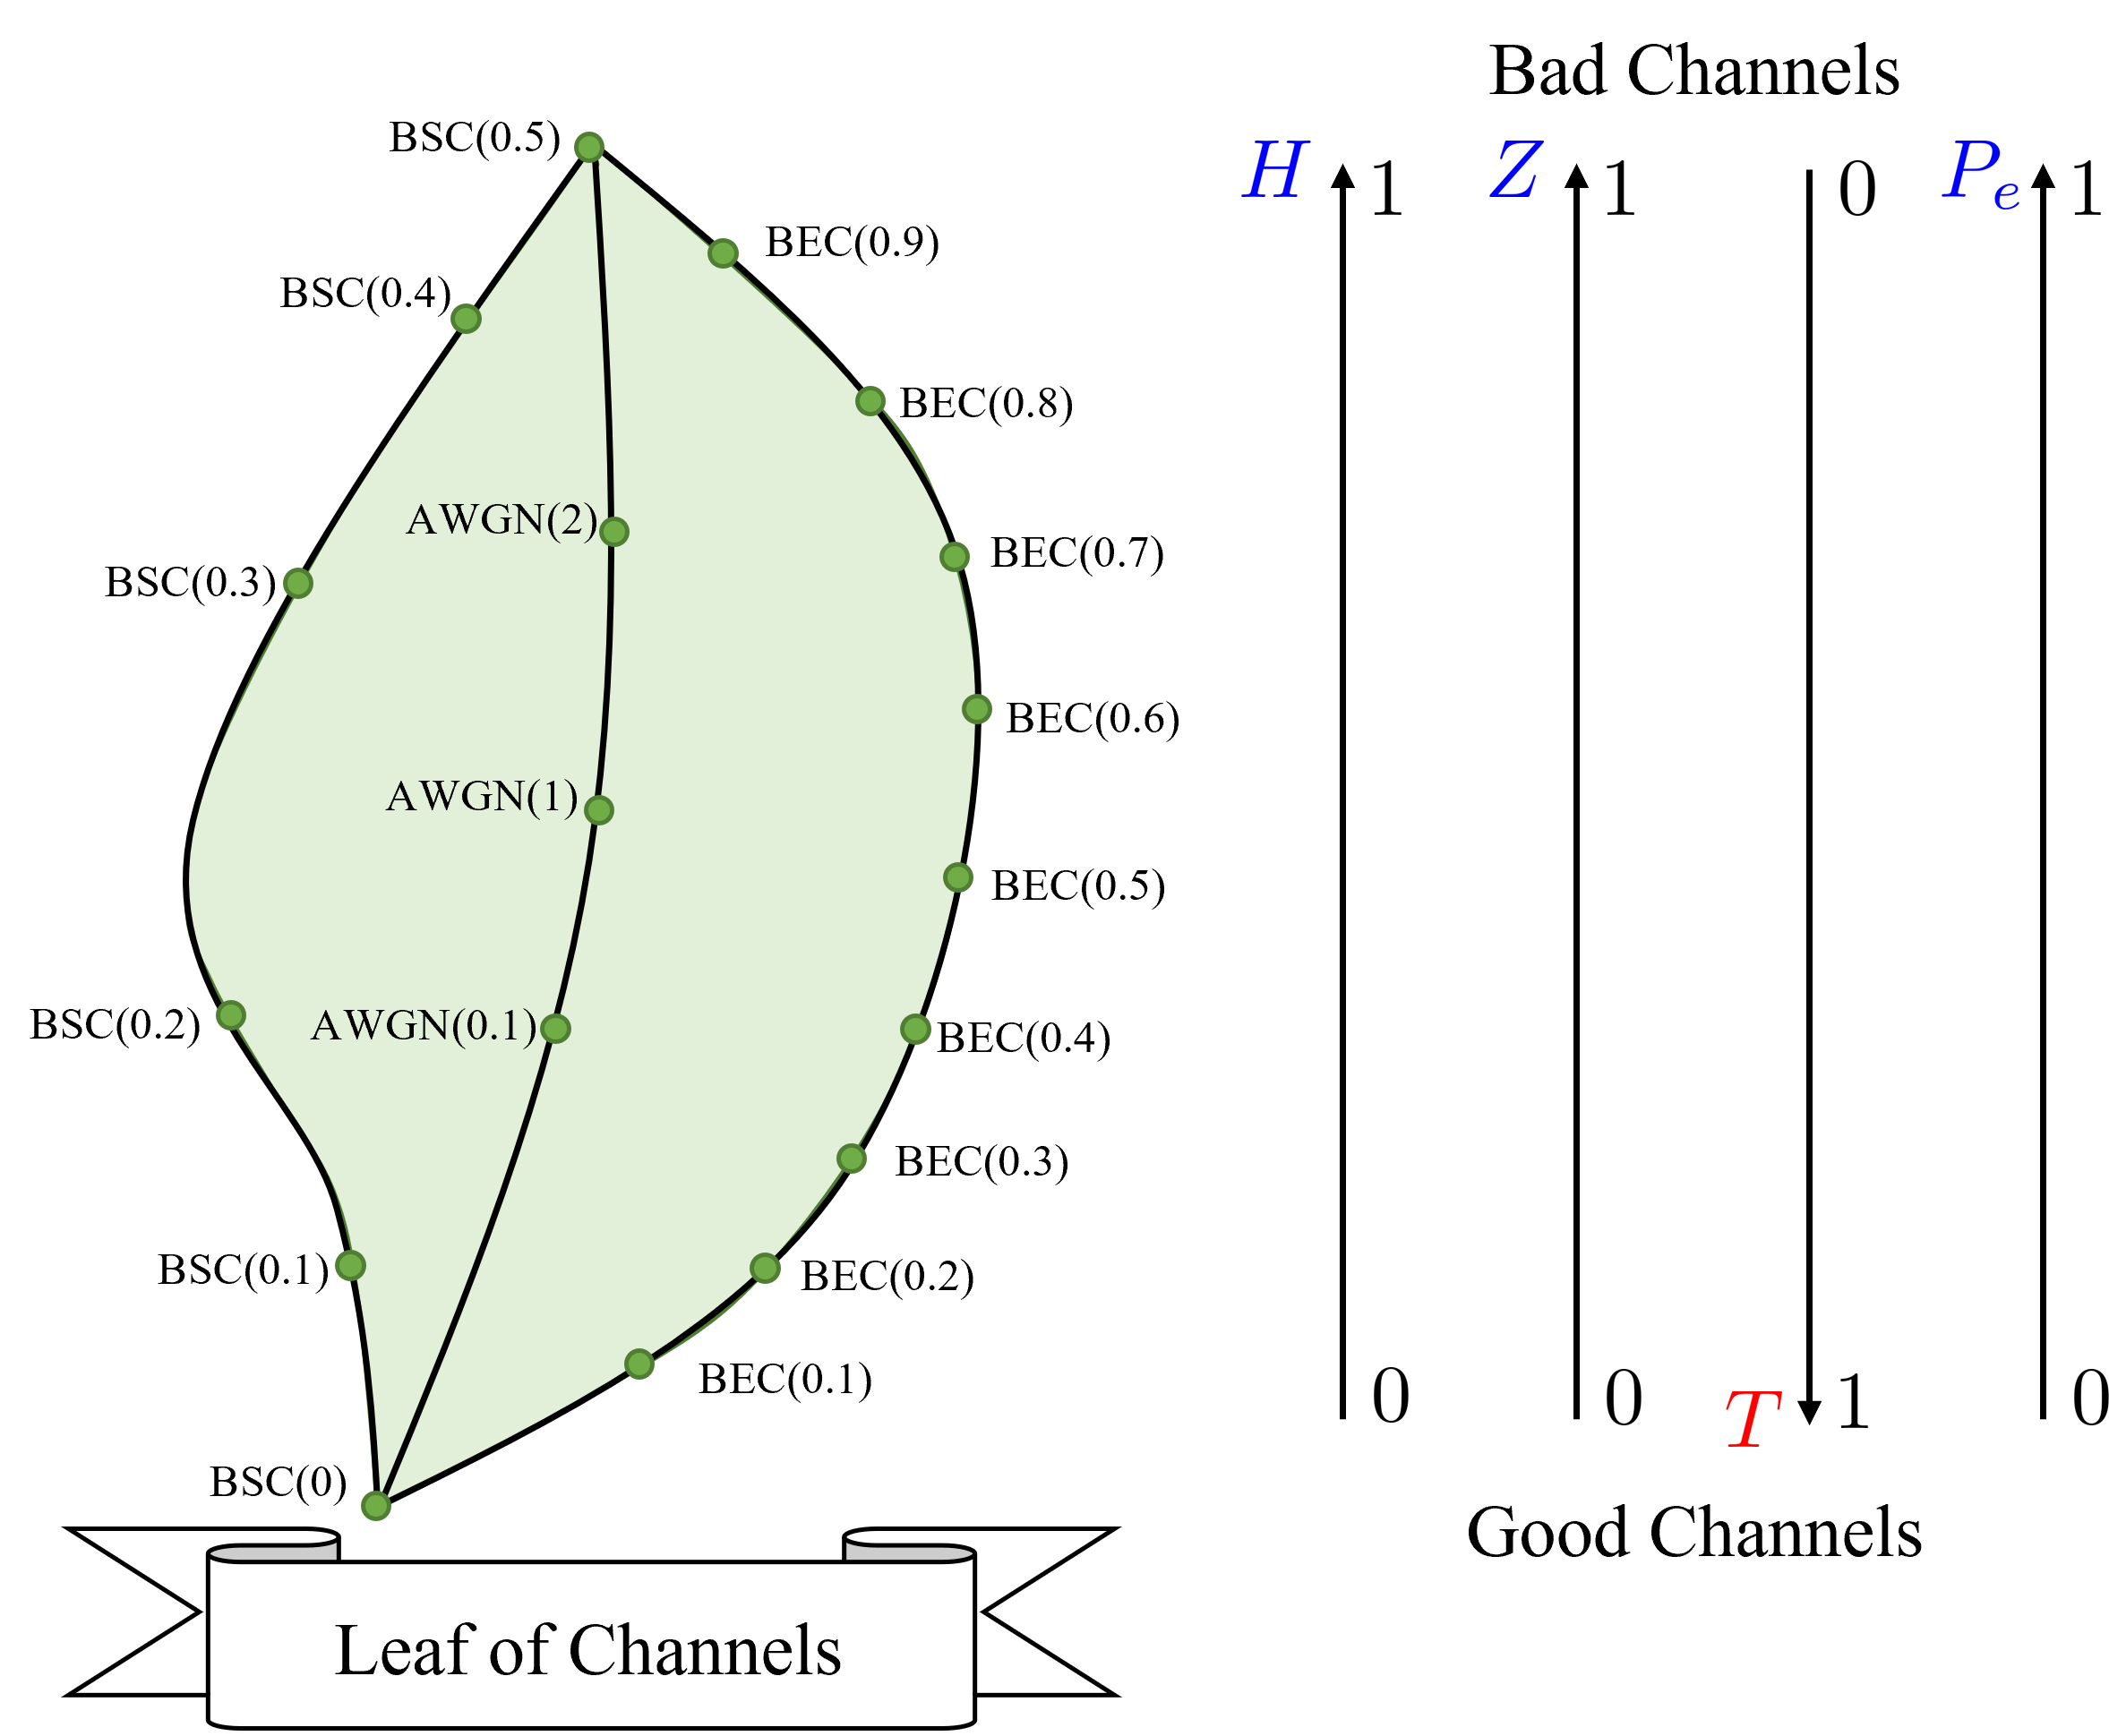
\includegraphics[width=0.8\linewidth]{figures/w5_leaf_of_channels.png}
    \caption{Leaf of channels representing the trend of channels from bad to good. The measures of the trend of how good a channel is are the channel parameters, coinciding on the value of 0 and 1 on $\mathrm{BSC}(0)$ and $\mathrm{BSC}(0.5)$ for the parameters $H$, $Z$, $P_e$ (measuring how bad a channel is), and vice versa for $T$.}
\end{figure}


\subsection{Inequalities of Channel Parameters}
For a more exhaustive list of results and proofs of the topic in this subsection, please refer to the papers ``A note on some inequalities used in channel polarization and polar coding'' \cite{Inequalities_Channel_Polarization} and ``Binary Polar Codes Based on Bit Error Probability'' \cite{Binary_PC_Bit_Err_Prob}.

\begin{theorem}
    For all BMSC $W$, we have
    \begin{equation}
        Z(W)^2\le H(W) \le Z(W).
    \end{equation}
\end{theorem}
\begin{proof}
    By plotting the respective values for the simple case $W=\mathrm{BSC}(p)$, we can see the above inequality holds true. Furthermore, the two inequalities still holds true under convex combination, but the first needs to further utilize the fact that $y=x^2$ is a convex functions.
\end{proof}
\begin{theorem}
    For a BMSC $W$,
    \begin{equation}
        1-T(W) \le H(W) \le h_b\left(\frac{1-T(W)}{2}\right)
    \end{equation}
\end{theorem}
\begin{proof}
    The proof is similar to the previous one, where one first show the inequality holds for BSCs, which is trivial. Then the first inequality is easily extended under convex combination. The second inequality still holds true since $h_b(p)$ is concave.
\end{proof}

\begin{remark}
    BEC is really special in that its $H=Z=P_e=1-T$ for all possible erasure probabilities.

    This is easy to show since that BECs are convex combination of the extremal BSCs, i.e., $\mathrm{BSC}(0)$ and $\mathrm{BSC}(1/2)$. The channel parameters coincide on these extremals.
\end{remark}

With the two inequalities above, we can actually bound regions of possible $(H,Z)$ and $(H,T)$ pairs as shown in \autoref{fig:w5_channel_parameter_region} below. Note that the upper curve in the $H$-$Z$ plot is not $Z^2=X$, it is not optimal.

\begin{figure}[H]
   \centering
   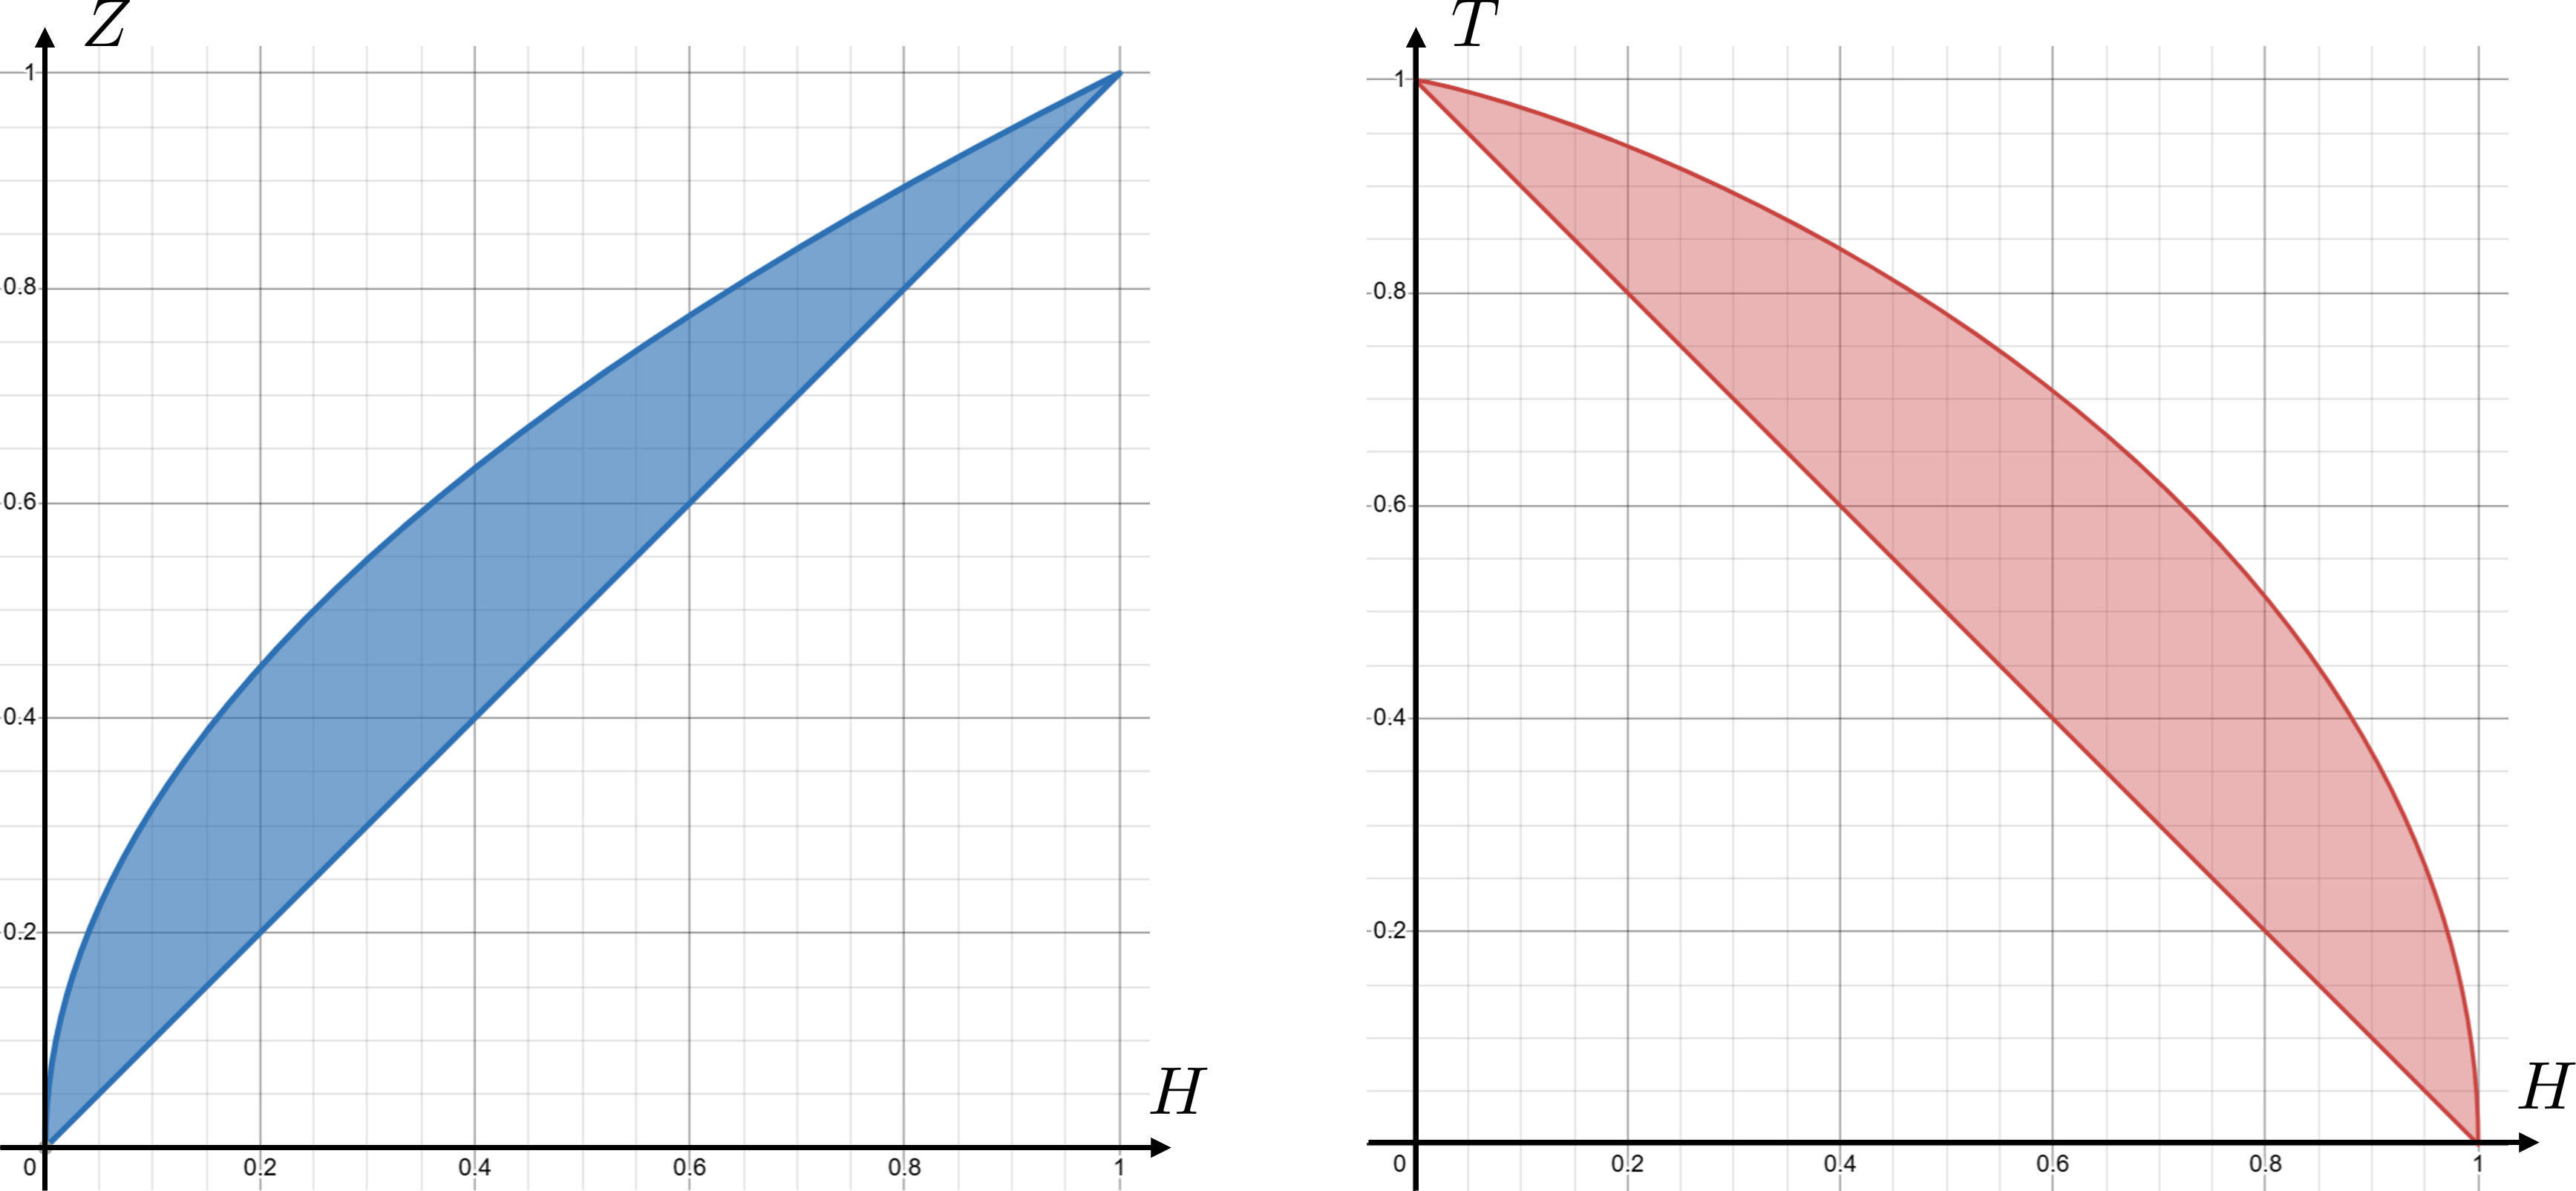
\includegraphics[width=0.8\linewidth]{figures/w5_region_parameter.png}
   \caption{Possible combinations of channel parameters.}
   \label{fig:w5_channel_parameter_region}
\end{figure}


\subsection{Channel Parameters as Martingales} 
Why do we study all these parameters? Because each one of them is good at one or two aspects, and only when combined together do we learn the full picture.
\begin{theorem}[Channel Parameters of Polarized Sub-Channels] \label{thm:channel_param_martingale}
    The following relations hold for the polarized sub-channels $W^+$ and $W^-$ of the BMSC $W$:
    \begin{align}
        &H(W^+) + H(W^-) = 2H(W),\\
        &Z(W^+) = Z(W)^2,\\
        &Z(W^-) \le 2Z(W) - Z(W)^2,\\
        &T(W^-) = T(W)^2,\\
        &T(W^+) \le 2T(W) - T(W)^2.
    \end{align}
    Hence, we know that for $s_{1:k}\in\{+,-\}^k$ $H(W^{s_{1:k}})$ is a martingale, and both $Z(W^{s_{1:k}})$ and $T(W^{s_{1:k}})$ are supermartingales. Furthermore, we have the more general results of
    \begin{align}
        Z(W_1\ostar W_2) &= Z(W_1)\cdot Z(W_2), \\
        T(W_1\boxstar W_2) &= T(W_1)\cdot T(W_2)
    \end{align}
    for channels $W_1$ and $W_2$.
\end{theorem}

\begin{remark}[Helliger Affinity]
    The Helliger affinity of a channel $W$ is defined as
    \begin{equation}
        Z_\alpha(W) = 2p^\alpha \bar{p}^{1-\alpha}.
    \end{equation}
    It is a (R\'enyi-like) generalization to the Bhatacharyya parameter (at $\alpha=1/2)$, also satisfying the multiplicative property of
    \begin{equation}
        Z_\alpha(W_1\ostar W_2) = Z_\alpha(W_1)\cdot Z_\alpha(W_2).
    \end{equation}
\end{remark}

The proof to parts of Theorem \autoref{thm:channel_param_martingale} will be shown later. But for now, let us analyze the consequences the martingales generated by the polarization process brought.
\begin{theorem}[Martingale Convergence Theorem]
    If $\{M_t\}$ is a bounded\footnote{For supermartingales $M_t$, the boundedness is in the sense of that $\sup_t \mathbb{E}[-\min(M_t,0)]<\infty$.} supermartingale / submartingale, then its limit exists: $M_t\xrightarrow{\text{a.s / $L^1$}}M_\infty$.
\end{theorem}
\begin{theorem}[Optional Stopping Time]
    For supermartingale $\{M_t\}$, we have $\mathbb{E}[M_\sigma] \le M_0$.

    For submartingale $\{M_t\}$, we have $\mathbb{E}[M_\sigma] \ge M_0$.
\end{theorem}
\begin{theorem}[Doob's Maximum Inequality]
    If $M_t\ge 0$ is a supermartingale, then $\mathrm{Pr}\{\max_tM_t\ge B\} \le M_0/B$.

    If $M_t\le 0$ is a submartingale, then $\mathrm{Pr}\{\max_tM_t\le -B\} \le -M_0/B$.
\end{theorem}

When applied to the channel parameters, one can have the following analyses:
\begin{example}
    Take the Bhattacharyya parameter as an example, define the Bhattacharyya martingale as
    \begin{equation}
        Z_0\defeq Z(W),\;Z_k\defeq Z(W^{s_{1:k}})\;\;\;\;\;(s^k\in\{+,-\}^k \text{ uniformly and random}).
    \end{equation}
    By the martingale convergence theorem, a limit should exist. It can be shown that $Z_\infty\in\{0,1\}$. Then we have
    \begin{equation*}
        \mathrm{Pr}\{Z_\infty=1\} = H_0 = H(W) \le Z_0.
    \end{equation*}
    Weirdly enough, one would expect the left hand side be equal to $Z_0$ by mirroring the proof from martingale. However, since now $Z_k$ is a supermartingale, the analysis should be: since $Z(W)\approx1$ if and only if $H(W)\approx 1$, we have
    \begin{equation}
        \mathrm{Pr}\{Z_\infty=1\} = \mathrm{Pr}\{H_\infty=1\} = H_0.
    \end{equation}
\end{example}

In fact, we have
\begin{equation}
    H_\infty = Z_\infty = 1 - T_\infty = P_{e,\infty}.
\end{equation}
Similarly, we have that as $k\rightarrow\infty$, $T_k$ converges to $T_\infty\in\{0,1\}$, with $\mathrm{Pr}\{T_\infty=1\} = 1-H_0$.

\subsection{Polar Decoder under Parallel and Serial Combination} \label{sec:w5_polar_dec_par_ser}
The general decoding scheme for a polar decoder is abstractly illustrated as below:
\begin{figure}[H]
    \centering
    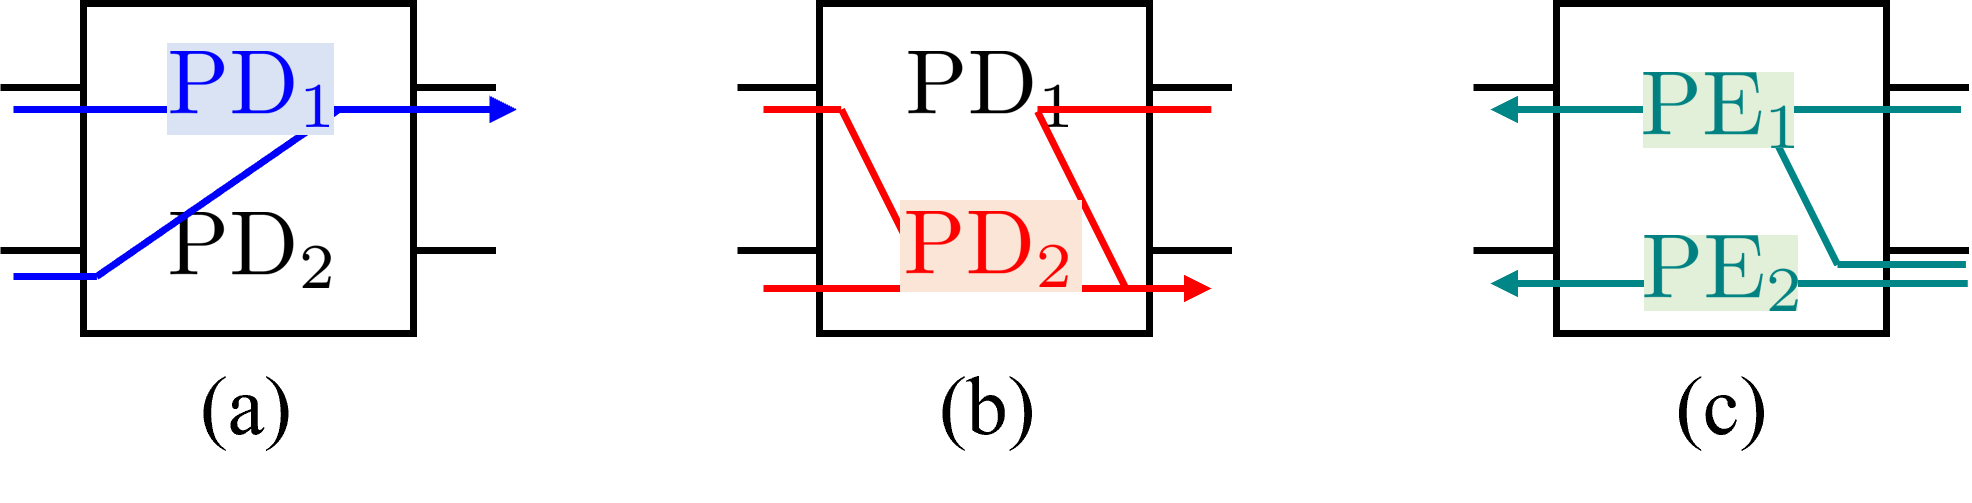
\includegraphics[width=0.6\linewidth]{figures/w5_dec_scheme.png}
    \caption{The three steps for decoding of polar code.}
\end{figure}
The decoding steps are implemented in real life by analyzing the likelihood ratio. To derive the likelihood ratio of the input symbols, let us introduce a new notion.
\begin{definition}[Posterior Probability Representation of Uncertain Symbols]
    If one were to guess the input $x\in\mathcal{X}=\{0,1\}$ given the received $y\in\mathcal{Y}$, the only crucial information are the posterior probabilities. Hence, one should represent $y$ by the pair of posterior probabilities
    \begin{equation}
        \left(W(0\vert y), W(1\vert y)\right)
    \end{equation}
    with a uniform prior, where the channel is $W:\mathcal{X}\rightarrow\mathcal{Y}$ .
\end{definition}

\begin{example}
    Consider the channel below:
    \begin{figure}[H]
        \centering
        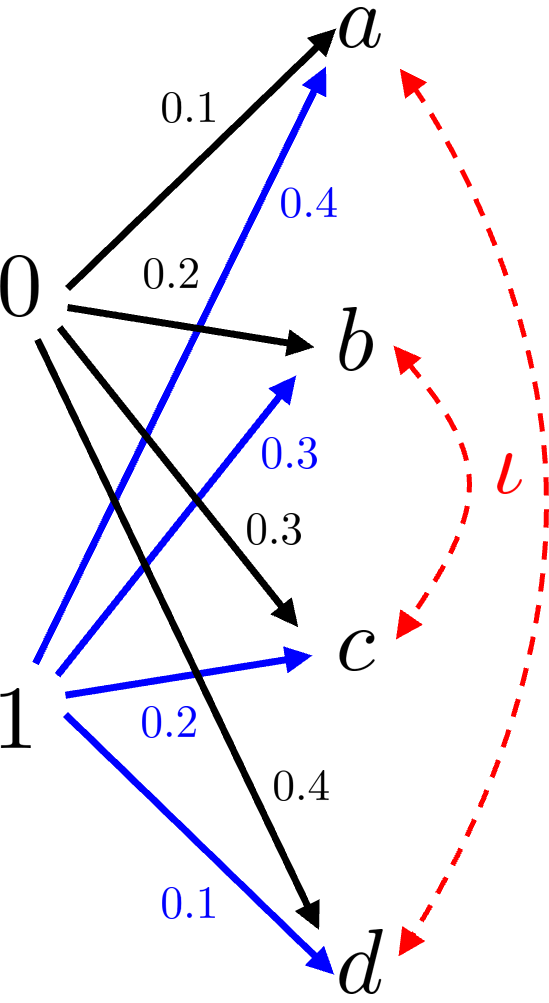
\includegraphics[width=0.2\linewidth]{figures/w5_post_rep1.png}
        \caption{Example of a BMSC for posterior representation.}
    \end{figure}
    In stead of ``$a$'', use the representation
    \begin{equation*}
        \left(W(0\vert a,W(1\vert a)\right) = \left(\frac{0.1}{0.1+0.4},\frac{0.4}{0.1+0.4}\right) = \left(\frac{1}{5},\frac{4}{5}\right).
    \end{equation*}
    Similarly, instead of ``$b$'', use $(2/5,3/5)$; instead of ``$c$'', use $(3/5,2/5)$; instead of ``$d$'', use $(4/5,1/5)$.
\end{example}
\begin{example}
    Consider the channel below
    \begin{figure}[H]
        \centering
        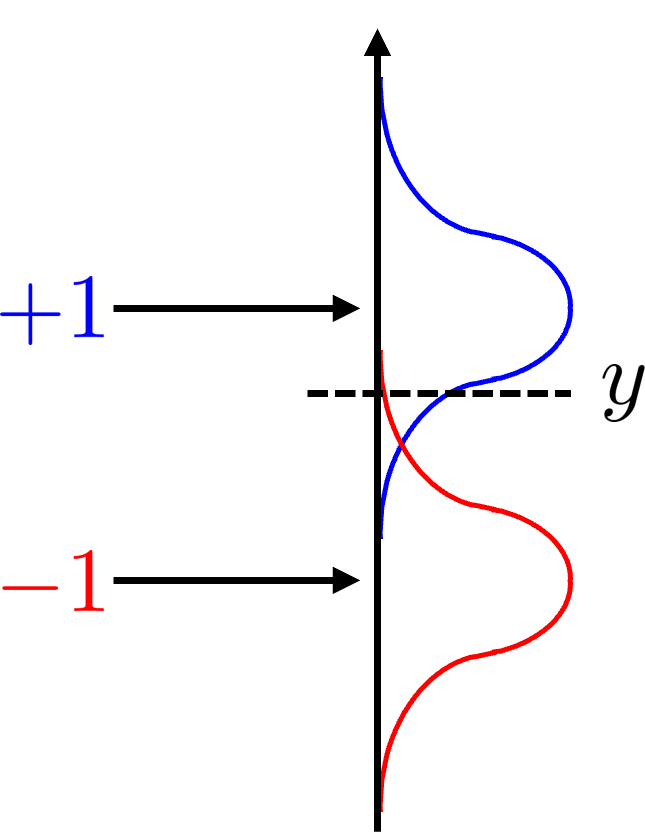
\includegraphics[width=0.2\linewidth]{figures/w5_post_rep2.png}
        \caption{Example of posterior representation on continuous random variables.}
    \end{figure}
    Since probabilities of outputs no longer make sense, we utilize the probability densities instead. Let the $\varphi(y)$ be the probability density function of the standard normal distribution. Then since $W(y\vert1)=\varphi(y-1)$ and $W(y\vert-1)=\varphi(y+1)$, we have the posterior representation of the output $y$ being
    \begin{equation*}
        \left(W(1\vert y),W(-1\vert y)\right) = \left(\frac{\varphi(y-1)}{\varphi(y-1)+\varphi(y+1)},\frac{\varphi(y+1)}{\varphi(y-1)+\varphi(y+1)}\right).
    \end{equation*}
\end{example}
Now let utilize both the posterior representation and the channel parameters introduced in the analysis of parallel and serial combination of channels.

\paragraph{Posterior Representation \& Parallel Combination:}

If one sends $X=x$ through $W$ and $W'$, and obtained posterior representations $(\alpha,\bar{\alpha})$ and $(\beta,\bar{\beta})$, respectively. Then what is the posterior probability of $x$ now? This can be readily solved by pretending $W$ and $W'$ as BSCs, and consider the figure below:
\begin{figure}[H]
    \centering
    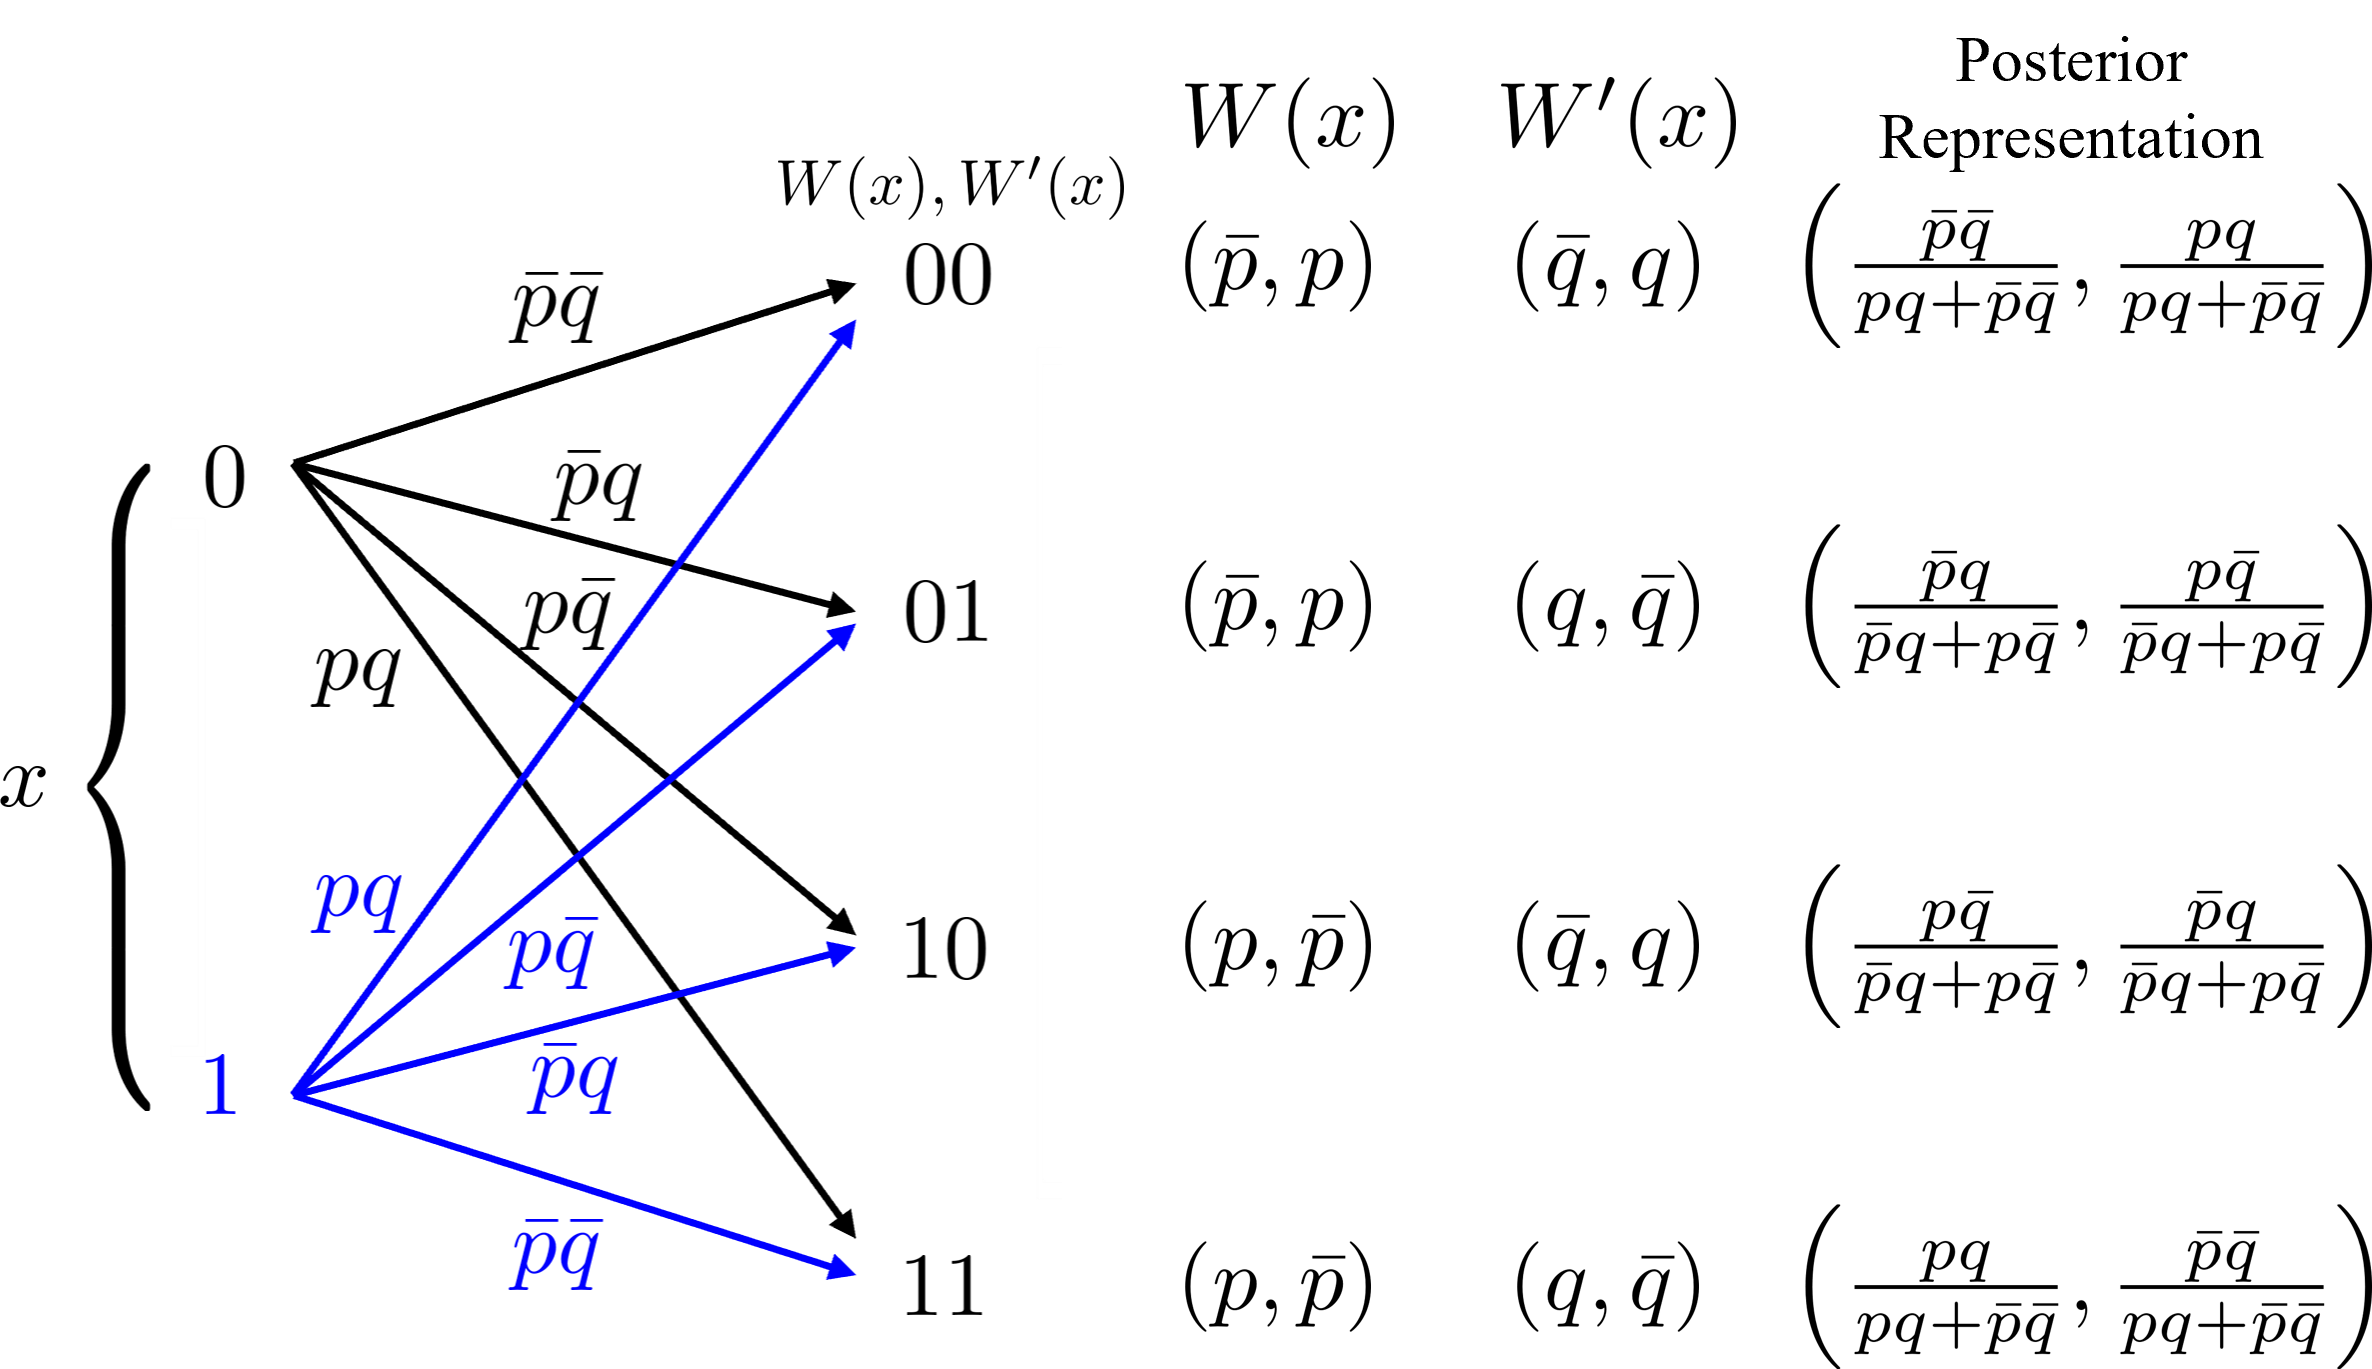
\includegraphics[width=0.7\linewidth]{figures/w5_post_parallel.png}
    \caption{Posterior representation for parallel combination of BSC's.}
\end{figure}
It is easily seen that if the received symbols are $(\alpha,\bar{\alpha})$ and $(\beta,\bar{\beta})$, they amount to a posterior representation of
\begin{equation}
    (\gamma,\bar{\gamma}) \defeq \left(W(x=0\vert W(x),W'(x)), W(x=1\vert W(x),W'(x))\right) = \left(\frac{\alpha\beta}{\alpha\beta + \bar{\alpha}\bar{\beta}} , \frac{\bar{\alpha}\bar{\beta}}{\alpha\beta + \bar{\alpha}\bar{\beta}}\right).
\end{equation}
Consider the likelihood ratios, especially, we can easily see that they are multiplicative!
\begin{equation}
    \frac{\gamma}{\bar{\gamma}} = \frac{\alpha}{\bar{\alpha}} \cdot \frac{\beta}{\bar{\beta}}.
\end{equation}
This serves as a mnemonic for one to remember the channel combination rule.

We hence have the following result:
\begin{theorem}[Bhattacharyya Parameter under Parallel Combination]
    For channels $W_1$ and $W_2$, we have
    \begin{equation}
        Z(W_1\ostar W_2) = Z(W_1)\cdot Z(W_2).
    \end{equation}
    Especially when $W_1=W_2=W$, we have
    \begin{equation}
        Z(W^+) = Z(W)^2.
    \end{equation}
\end{theorem}
\begin{proof}
    Since any BMSC can be decomposed into a convex combination of BSCs, we only need to proof the theorem above for parallel combination of BSCs. This can be directly proven by plugging in \autoref{w3:BSC_parallel}. 
    
    However, also observe that for a general channel $W=\sum_i a_i \mathrm{BSC}(p_i)$. By treating the output symbols $y_i$ in their posterior representations $(\alpha(y_i),\bar{\alpha}(y_i)) = (p_i,\bar{p}_i)$ as a random variable with distribution derived from sending only 1 as the input, we can construct the following expectation:
    \begin{equation*}
        Z(W) = \sum_i a_i\cdot2\sqrt{p_i\bar{p}_i} = \sum_i a_i\left(p_i\sqrt{\bar{p}_i/p_i} + \bar{p}_i \sqrt{p_i/\bar{p}_i}\right) = \mathbb{E}\left[\sqrt{\bar{\alpha}/\alpha}\right].
    \end{equation*}
    Then the result above can be simply derived from
    \begin{equation*}
        Z(W_1\ostar W_2) = \mathbb{E}\left[\sqrt{\gamma/\bar{\gamma}}\right] = \mathbb{E}\left[\sqrt{\alpha/\bar{\alpha}}\right] \cdot \mathbb{E}\left[\sqrt{\beta/\bar{\beta}}\right] = Z(W_1) \cdot Z(W_2).
    \end{equation*}
\end{proof}


\paragraph{Posterior Representation \& Serial Combination:}

If one sent $x$ through $W$ obtaining $(\alpha,\bar{\alpha})$ and sent $y$ through $W'$ obtaining $(\beta,\bar{\beta})$. Then what is the posterior representation to $x+y$? Similarly, pretend $W$ and $W'$ to be BSCs and consider the figure below:
\begin{figure}[H]
    \centering
    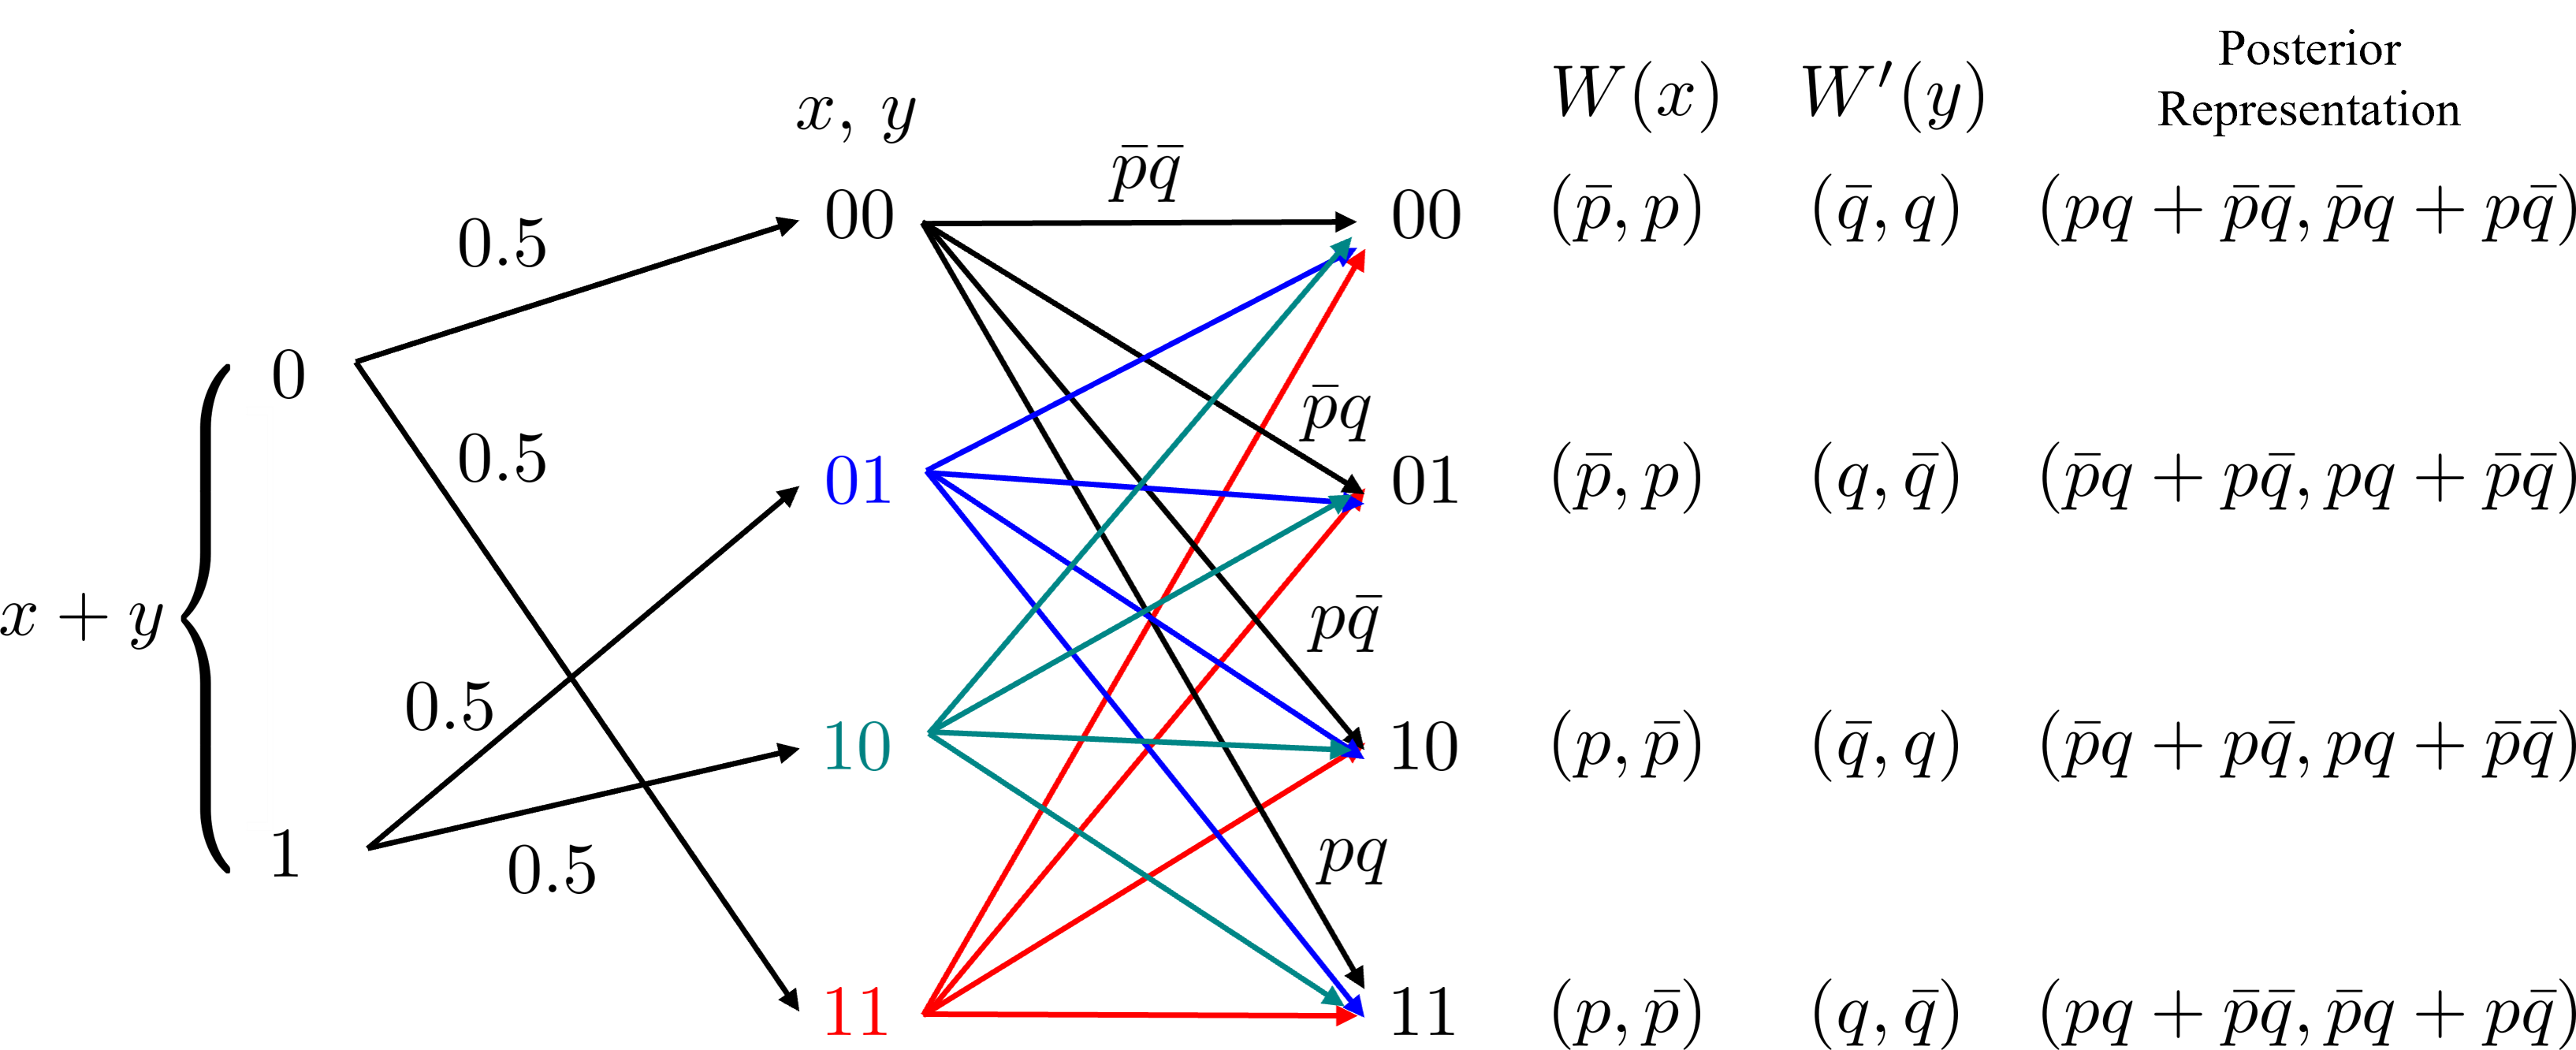
\includegraphics[width=0.9\linewidth]{figures/w5_post_serial.png}
    \caption{Posterior representation for serial combination of BSC's.}
\end{figure}
One can see that if the received symbols are $(\alpha,\bar{\alpha})$ and $(\beta,\bar{\beta})$, they amount to a posterior representation of
\begin{equation}
    (\gamma,\bar{\gamma}) \defeq \left(W(x+y=0\vert W(x),W'(y)), W(x+y=1\vert W(x),W'(y))\right) = \left(\alpha\beta + \bar{\alpha}\bar{\beta},\bar{\alpha}\beta + \alpha\bar{\beta}\right).
\end{equation}
One can also observe that the signed variation distance is multiplied:
\begin{equation}
    (\gamma-\bar{\gamma}) = (\alpha-\bar{\alpha}) \cdot (\beta-\bar{\beta}).
\end{equation}
This serves as yet another mnemonic.

The following result follows suit:
\begin{theorem}{Total Variation Distance under Serial Combination} \label{thm:w5_TV_multiply}
    For channels $W_1$ and $W_2$, we have
    \begin{equation}
        T(W_1\boxstar W_2) = T(W_1) \cdot T(W_2).
    \end{equation}
    Especially when $W_1=W_2=W$, we have
    \begin{equation}
        T(W^-) = T(W)^2.
    \end{equation}
\end{theorem}
\begin{proof}
    Again, we only need to proof the theorem above for serial combination of BSCs, and can be directly proven by plugging in \autoref{w3:BSC_serial}. However, the proof can also be done by constructing a random variable. Treating $(\alpha,\bar{\alpha})$ as a random variable following the distribution as sending only 1 through as input, then
    \begin{align*}
        \rightarrow T(W) &= \sum_{i} a_i \abs{p_i-\bar{p}_i} = \sum_i a_i \left(\bar{\alpha}(y_i) \abs{\alpha(y_i)-\bar{\alpha}(y_i)} + {\alpha}(y_i) \abs{\bar{\alpha}(y_i)-{\alpha}(y_i)}\right) \\
        &= \mathbb{E}\left[\abs{\alpha-\bar{\alpha}}\right].
    \end{align*}
    Hence,
    \begin{align*}
        T(W_1\boxstar W_2) = \mathbb{E}\left[\abs{\gamma-\bar{\gamma}}\right] = \mathbb{E}\left[\abs{\alpha-\bar{\alpha}}\right] \cdot \mathbb{E}\left[\abs{\beta-\bar{\beta}}\right] = T(W_1)\cdot T(W_2).
    \end{align*}
\end{proof}


In real applications, which representation is used? $(\alpha,\bar{\alpha})$, $\alpha/\bar{\alpha}$, or $\alpha-\bar{\alpha}$? The answer is that the log likelihood ratio (LLR) is used.

It is easy to see that under parallel combination, we have
\begin{equation}
    \mathrm{LLR}_\gamma = \mathrm{LLR}_\alpha + \mathrm{LLR}_\beta, \label{eq:w5_LLR_add}
\end{equation}
where $\mathrm{LLR}_\alpha = \ln(\alpha/\bar{\alpha})$. The additive property makes the calculation of channel parallel combination very easy. How about serial combination?

Under serial combination, we have that
\begin{equation}
    \mathrm{LLR}_\gamma = 2 \arctanh\left(\tanh\left(\mathrm{LLR}_\alpha/2\right) + \tanh\left(\mathrm{LLR}_\beta/2\right)\right).
\end{equation}
This can be easily seen by following the calculations below:
\begin{align*}
    &\because \alpha/\bar{\alpha} = \exp(\mathrm{LLR}_\alpha) \Rightarrow \bar{\alpha} = \frac{1}{1+\exp(\mathrm{LLR}_\alpha)} \\
    &\therefore \gamma-\bar{\gamma} = \frac{\exp(\mathrm{LLR}_\gamma) - 1}{\exp(\mathrm{LLR}_\gamma) + 1} = \frac{\exp(\mathrm{LLR}_\alpha) - 1}{\exp(\mathrm{LLR}_\alpha) + 1} \cdot \frac{\exp(\mathrm{LLR}_\beta) - 1}{\exp(\mathrm{LLR}_\beta) + 1} = (\alpha-\bar{\alpha})\cdot(\beta-\bar{\beta}) \\
    &\Rightarrow \tanh(\mathrm{LLR}_\gamma/2) = \tanh(\mathrm{LLR}_\alpha/2) \cdot \tanh(\mathrm{LLR}_\beta/2).
\end{align*}
Thus the relation is shown.

The two rules above constitutes the famous ``product-sum rule.'' Moreover, since hyperbolic-(arc)tangent is costly to compute, as simpler approximation formula exists:
\begin{equation}
    \mathrm{LLR}_\gamma \approx \mathrm{sgn(\mathrm{LLR}_\alpha\cdot\mathrm{LLR}_\beta}) \cdot \min\left\{\abs{\mathrm{LLR}_\alpha},\abs{\mathrm{LLR}_\beta}\right\}.
\end{equation}

\begin{figure}[H]
    \centering
    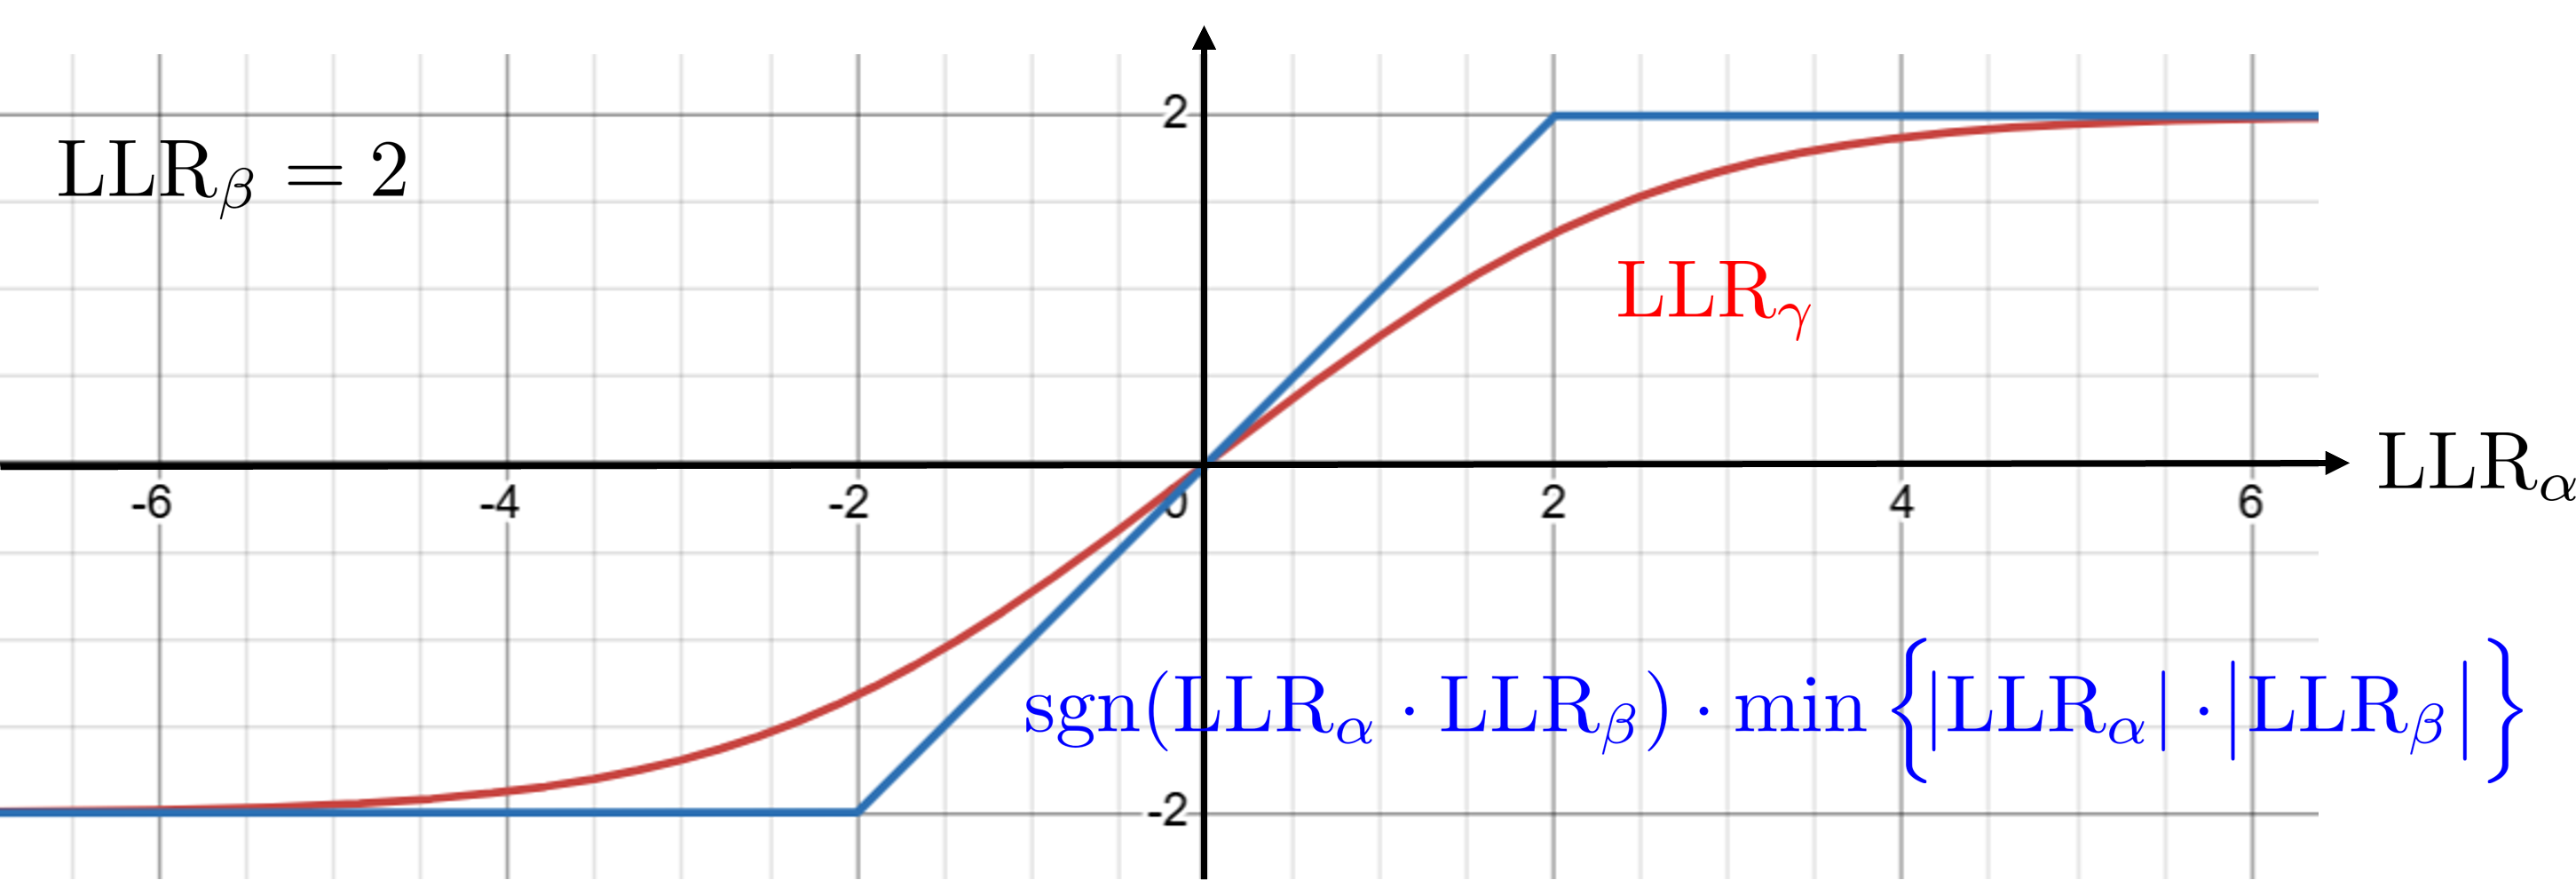
\includegraphics[width=0.7\linewidth]{figures/w5_approx_LLR.png}
    \caption{Approximation for the LLR of serial combination.}
\end{figure}

\begin{example}
    If one flips a biased coin with probability of landing on heads being $p$ a total of $n$ times, what is the probability that the number of heads obtained is even?

    This problem can be solved by using techniques from difference equations. However, we can recast this problem into a channel: Suppose one transmits the bit string $00\ldots 0$ (length $n$) through a $W=\mathrm{BSC}(p)$, then the probability of receiving obtaining an even amount of 1's is the same as the probability in question. This then also equals to the probability that summing (mod 2 summation) the received bits gives you 0. The summation of received bits is equivalent to the serial combination of channels! Since the signed total variation distance (temporarily denoted by $\tilde{T}$) is multiplicative under serial combination, let the probability of obtaining a sum of 0 be denoted by $q$, then
    \begin{equation*}
        \tilde{T}(W^{\boxstar n}) = q - (1-q) = \left((1-p) - p\right)^n = \tilde{T}(W)^n \Rightarrow q = \frac{1}{2}\left((1-2p)^{n} + 1\right).
    \end{equation*}
\end{example}

\section{Distributed Source Coding}
This section discusses the possibility of distributed source coding by the method of Slepian-Wolf.

\begin{figure}[H]
    \centering
    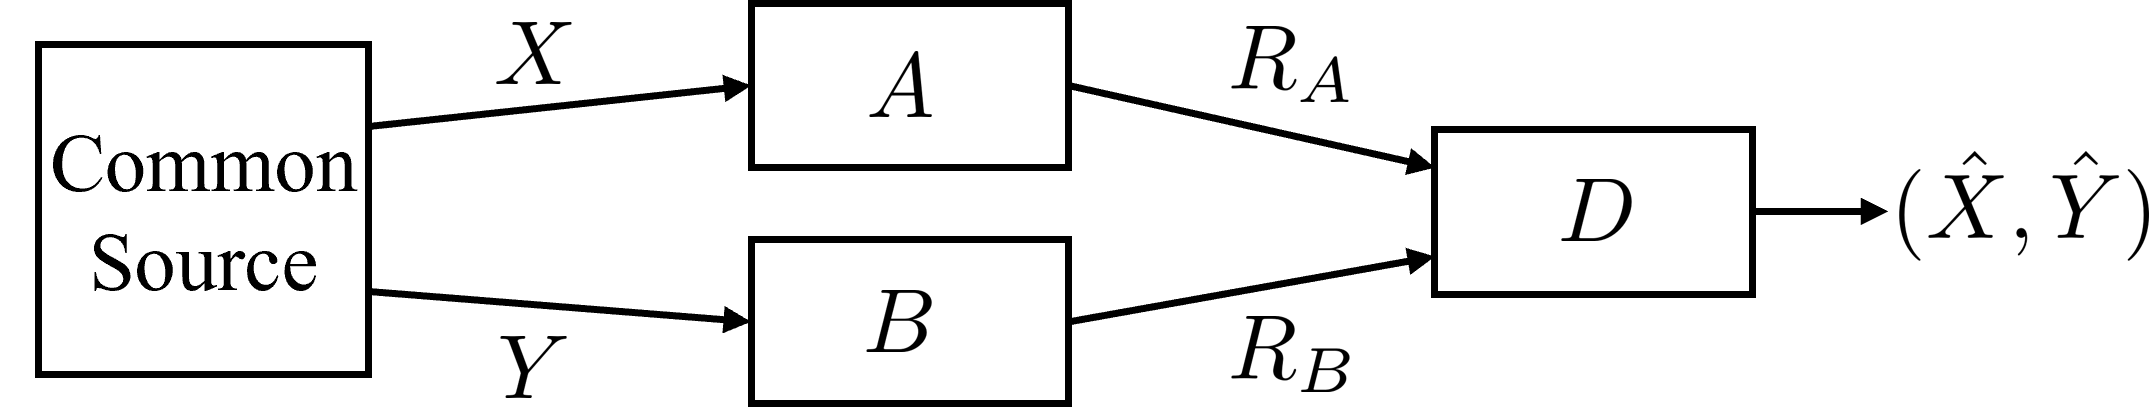
\includegraphics[width=0.6\linewidth]{figures/w5_distr_src_coding.png}
    \caption{Distributed source coding of a common source by two agents $A$ and $B$.}
\end{figure}

Consider the figure above: agent Alice ($A$) and Bob ($B$) has a common source and plan to send bit streams with rate $R_A$ and $R_B$ to decoder David ($D$) to learn about the source. What are the possible $(R_A,R_B)$ pairs?

From \autoref{sec:slepian_wolf_1}, we have learned that if Alice or Bob shares information with the other (say, Alice knows about the random variable $Y$ that Bob obtains), then Alice can send at a rate of $H(X\vert Y)$ while Bob sends at a rate of $H(Y)$. But now our question is restricted so that there are no information exchange between Alice and Bob, is there a way for the them to compress their information while still enabling David to decode the information losslessly? Our task then will be to find a way to describe the \textit{rate region}.

\begin{definition}[Rate Region]
    The rate region is a subset $\mathcal{R}\subset\mathbb{R}^2$ such that $(R_A,R_B)\in\mathcal{R}$ is feasible.
\end{definition}

The characterization to the rate region is the figure below:
\begin{figure}[H]
    \centering
    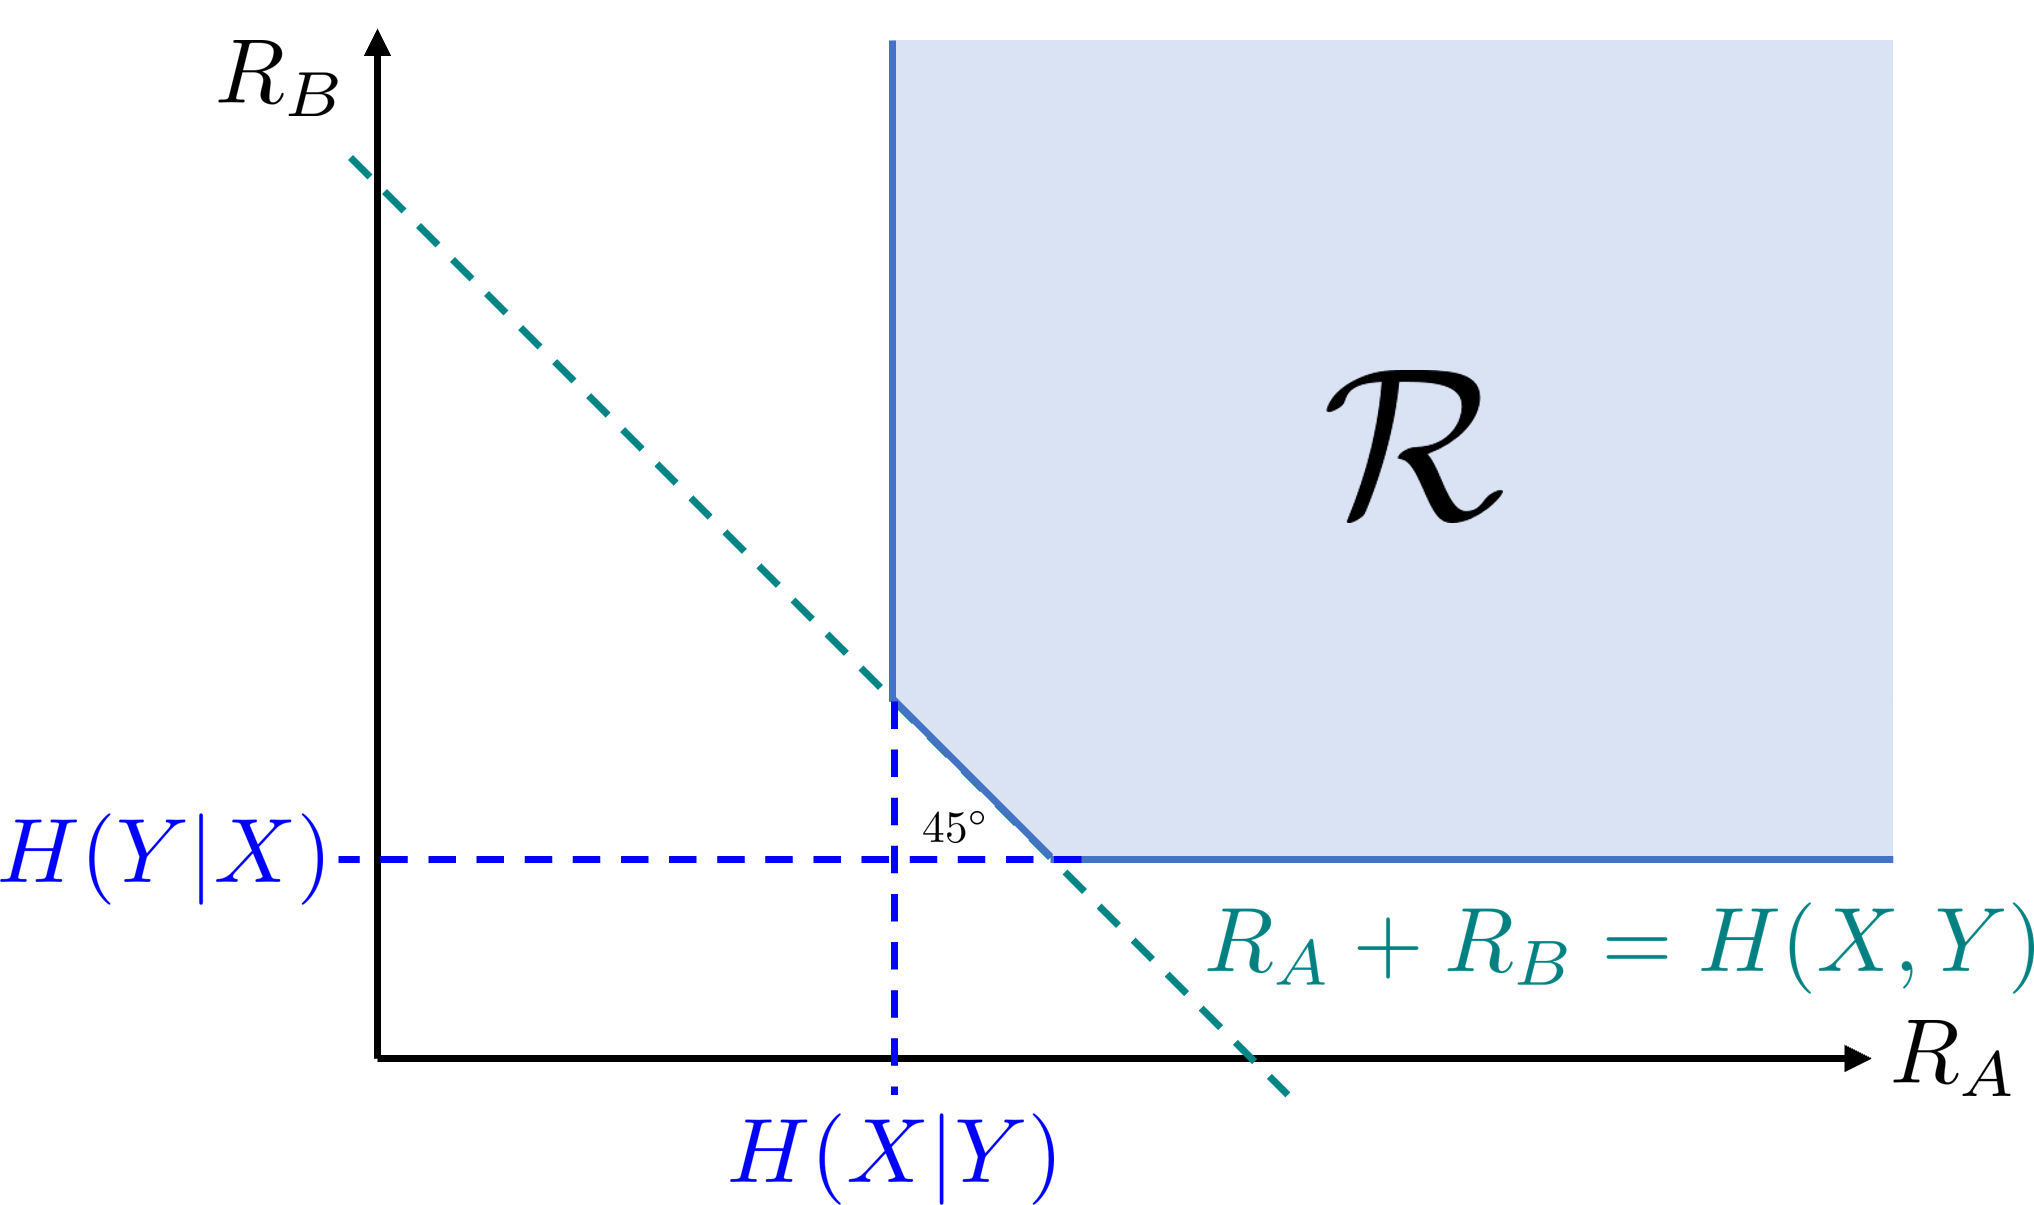
\includegraphics[width=0.6\linewidth]{figures/w5_slepian_wolf.png}
    \caption{Rate region of two agent distributed source coding.}
\end{figure}
\begin{remark}
    The more bits used to describe a single symbol, the more possible it is do decode. Hence, the region $\mathcal{R}$ is unbounded on the top right corner.

    If $X$ and $Y$ are independent, $H(Y\vert X) = H(Y)$ and $H(X\vert Y) = H(X)$, hence $H(X)+H(Y) = H(X,Y)$, the rate region simply becomes an unbounded rectangle.
\end{remark}

The strategy of the coding scheme for Alice and Bob is simple: ask Alice to send bit streams with a rate of $H(X\vert Y)$ and ask Bob to send with a rate of $H(Y)$. An immediate problem arises, however, without explicitly knowing the $Y$ Bob obtains, how can Alice compress the information? Luckily, this task is actually possible, and the technique used is called \textit{random binning}:
\begin{enumerate}
    \item Prepare $2^{n(H(X)+\varepsilon)}$ small balls for Alice. This corresponds to the typical set $\mathcal{A}(n,\varepsilon)$ of information in $X$. 
    \item Prepare $2^{n(H(X\vert Y)+\varepsilon)}$ large bins.
    \item Alice throws the balls into the bins randomly. (Note that if there is no side information, Shannon says that Alice should in fact send David the index of the balls which costs $n(H(X)+\varepsilon)$ bits.)
    \item Alice send the index of the bin a ball is in to David, costing $n(H(X\vert Y) +\varepsilon)$ bits.
    \item In order to show that this trick actually works, David should be able to find the correct ball that is in the bin which has an index Alice sent and David knows.
    \item Each ball is a different random stream of variable $X_{1:n}$. David will select the ball with the largest probability $\mathrm{Pr}\{X_{1:n}\vert Y_{1:n}\}$.
    \item Control and bound the error probabilities:
    \begin{itemize}
        \item The wrong ball has a higher probability.
        \item $\cdots$ (to be left as an exercise for the readers)
    \end{itemize}
\end{enumerate}
By bounding the error probabilities, we can show that the strategy of random binning is feasible, and the error probabilities reaches zero as $n$ becomes asymptotically large.
\section{Speed of Polarization}
\lecture{25 Mar.}

Referring back to Theorem \ref{thm:w1_polar_speed}, where we established the speed at which BECs polarize. Now let us delve deeper into the analysis and show some of the missing details while connecting with what we have learned. The papers ``Unified Scaling of Polar Codes: Error Exponent, Scaling Exponent, Moderate Deviations, and Error Floors'' \cite{Unified_Scaling_of_Polar_Codes} and ``Sub-4.7 Scaling Exponent of Polar Codes'' \cite{Sub_4_7_Scaling_Exponent} provide more recent advances in finding the scaling exponent and its relationship with other coding theoretical parameters.

Let us assume that there exists a special concave function $f(x)$ (an approximation would be $\approx[x(1-x)]^{2/3}$, with another commonly used exponent is 0.7). By concavity, we have that
\begin{align*}
    &f(x^2) + f(2x-x^2) \le 2f(x) \\&\Rightarrow f\left(P_e(\mathrm{BEC}(x)^+)\right) + f\left(P_e(\mathrm{BEC}(x)^-)\right) \le 2 f\left(P_e(\mathrm{BEC}(x))\right).
\end{align*}
This is how this special function is linked with BECs. Furthermore, we are interested in the following quotient (see also the figure below) that is between 0 and 1:
\begin{equation}
    \lambda \defeq \sup_{0\le x\le 1} \frac{f(x^2) + f(2x-x^2)}{2f(x)}. \label{eq:w6_polarization_lambda}
\end{equation}

We have already shown that
\begin{equation}
    \frac{1}{2^n}\sum_{s\in\{+,-\}^n}f\left(P_e(\mathrm{BEC}(x)^s)\right) \le \lambda^n f(x).
\end{equation}
Hence as $n\rightarrow\infty$, we have that $f\left(P_e(\mathrm{BEC}(x)^s)\right)$ approaches 0 for all $s$, meaning that $P_e(\mathrm{BEC}(x)^s)=0$ or $1$ for all $s$. This is our characterization of the speed of polarization. 

For all possible convex $f$, which produces the smallest $\lambda$? It is obvious that for $[x(1-x)]^{2/3}$, the $\lambda$ is not optimal. How do we find the optimal $f$? Simply by the power method.

\begin{remark}
    Let us take a small detour into the ``power method'' from linear algebra, which is very similar to the question proposed above.

    Given a matrix $A$, we would like to find the eigenvalue with the largest absolute value, i.e.
    \begin{equation*}
        \abs{\lambda_1} = \max_{\vec{x}} \frac{\norm{Ax}}{\norm{x}},
    \end{equation*}
    where the norm is the Euclidean norm. The maximum is achieved when $\vec{x}=\vec{x}_1$, the eigenvector corresponding to the eigenvalue $\lambda_1$. A useful method in finding $\vec{x}$, and hence $\lambda_1$, is the power method, in which one simply iterates the map
    \begin{equation*}
        \vec{x} \leftarrow \varphi(\vec{x}) = \frac{A\vec{x}}{\norm{\vec{x}}}.
    \end{equation*}
    Then we have $\varphi^n(\vec{x})\rightarrow\vec{x}_1$ as $n\rightarrow\infty$.
\end{remark}

For BECs, let us define the following operator
\begin{equation}
    T_{\mathrm{BEC}}(f) = \frac{f(x^2)+f(2x-x^2)}{2}.
\end{equation}
% Since the erasure probability of BECs under the polarization process is a martingale,
% \begin{equation}
%     \mathbb{E}[f(P_{e,n)}\vert P_{e,0}] = \overbrace{T_{\mathrm{BEC}}\circ T_{\mathrm{BEC}}\circ\cdots\circ T_{\mathrm{BEC}}}^{n\text{ times}}(f).
% \end{equation}
Then \autoref{eq:w6_polarization_lambda} will be equivalent to finding the largest eigenvalue to the eigenvalue problem
\begin{equation}
    T_{\mathrm{BEC}}(f) = \lambda f(x).
\end{equation}
However, we always have the trivial largest eigenvalue of $\lambda=1$ for $f(x)=1$ and $f(x)=x$. Hence, we are to find the largest eigenvalue $\lambda^*$ other than $1$.


By the power method, we define the following iteration scheme:
\begin{equation}
    f \leftarrow \frac{f(x^2) + f(2x-x^2)}{2\sup_{x\in[0,1]}f(x)}. \label{eq:w6_polar_speed_fxn}
\end{equation}
In the end when this iteration converges, the supremum is $\lambda^*=2^{-1/\mu^*}$, the value $\mu^*$ is coined the scaling exponent.

\begin{figure}[H]
    \centering
    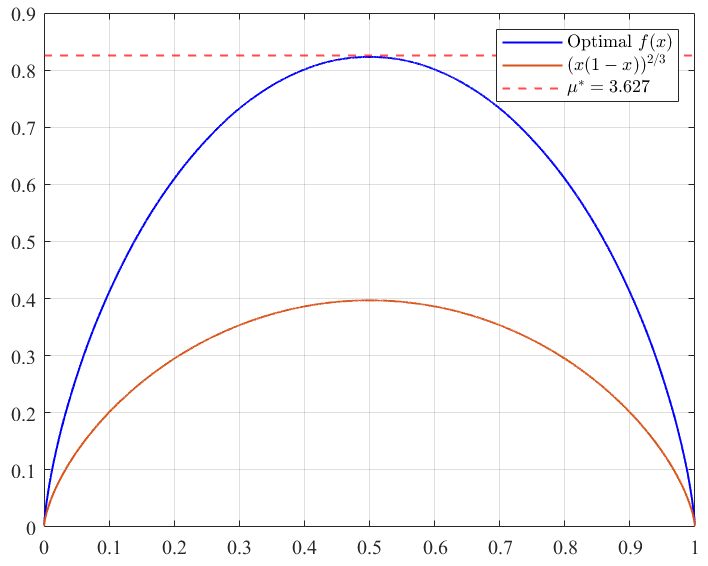
\includegraphics[width=0.6\linewidth]{figures/w6_polarization.png}
    \caption{Eigenfunction to $T_\mathrm{BEC}$.}
    \label{fig:w6_eigfxn}
\end{figure}

Using $(x(1-x))^{2/3}$ as the initial condition, the algorithm quickly converges to \autoref{fig:w6_eigfxn}, with the optimal scaling exponent equal to $\mu^*=3.627$.

\begin{remark}
    Why does \autoref{eq:w6_polar_speed_fxn} converge?
\end{remark}

Previously in \autoref{eq:w3_martingale_conv}, we considered $M_n$ as the polarization process of $\mathrm{BEC}(x)$, and by arguments of martingale convergence theorem, we have seen that
\begin{equation*}
    \mathrm{Pr}\{M_n\in(\varepsilon,1-\varepsilon)\} < \delta
\end{equation*}
is a constant bound on the converging probability. We can do better than this by introducing the optimal $f$ (optimal as in the arguments above) to have
\begin{align*}
    \mathrm{Pr}\{M_n\in(\varepsilon,1-\varepsilon)\} &= \mathrm{Pr}\{f(M_n) > f(\varepsilon)\} \\
    &\le \frac{\mathbb{E}[f(M_n)]}{f(\varepsilon)} \\
    &\approx 2^{-\frac{n}{3.627}} f(M_0) / f(\varepsilon).
\end{align*}
We can see that the speed of polarization is exponentially fast.

\begin{remark}
    Besides plugging in $x$ as the error probability, we have also learned that the Bhattacharyya parameter $Z$ as an equivalent description of channel quality! For BECs, the Bhattacharrya parameter $Z_n$ follows the same polarization process as $P_e$, and hence has the same polarization speed. 
    
    However, for more general BMSCs, the Bhattacharyya parameter becomes a supermartingale. By denoting $z=Z(W)$,
    \begin{equation}
        z\sqrt{2-z^2} \le Z(W^-) \le 2z-z^2,
    \end{equation}
    the iteration \autoref{eq:w6_polar_speed_fxn} hence needs to be updated as
    \begin{equation}
        f \leftarrow \sup_{x\sqrt{2-x^2} \le y \le 2x-x^2} \frac{f(x^2)+f(y)}{2\sup_{x\in[0,1]}f(x)}.
    \end{equation}
    In this case, the scaling exponent obtained will be $\mu^*=4.717$, just as described in \autoref{thm:w1_polar_speed}.
\end{remark}

\section{Large Kernel of Polar Code}
Previously in polar code, we have only been consider the $2\times 2$ kernel $\left[\begin{matrix}
    1 & 0 \\ 1 & 1
\end{matrix}\right]$ as proposed by Ar{\i}kan, where each encoding and decoding block has two input and two outputs. However, this can be modified to allow for a larger kernel.

If we consider
\begin{equation*}
    A = \left[\begin{matrix}
        a_{11} & \cdots & a_{\ell1} \\
        \vdots & \ddots & \vdots \\
        a_{1\ell} & \cdots & a_{\ell\ell}
    \end{matrix}\right] \in \mathbb{F}_2^{\ell\times\ell}
\end{equation*}
as our kernel for polar code, then given the input bits $[u_1,\ldots,u_\ell]$, the encoded bits will be $[x_1,\cdots,x_\ell] = [u_1,\ldots,u_\ell] A$. With the encoded bits as channel inputs, the channel outputs will be $[y_1,\cdots,y_\ell]$. The decoder is again operated by maximum likelihood estimation. The $\ell$ polarized channels will be:
\begin{itemize}
    \item $W^{(1)}$ is guessing $u_1$ given $y_1,\ldots,y_\ell$.
    \item $W^{(2)}$ is guessing $u_2$ given $y_1,\ldots,y_\ell$ and $u_1$.
    \item $W^{(3)}$ is guessing $u_3$ given $y_1,\ldots,y_\ell$ and $u_1,u_2$.
    \item $\vdots$
    \item $W^{(\ell)}$ is guessing $u_\ell$ given $y_1,\ldots,y_\ell$ and $u_1,\ldots,u_{\ell-1}$.
\end{itemize}
The matrix $A$ is termed the \textit{generator matrix} of the code. For more details, and also for the definitions of the terms used in the theorem below, please refer to \autoref{sec:w6_algebra}.

\begin{theorem}
    Consider a code with generator matrix $A$ for a BMSC $W$. Let $A_i$ be the $i$th row to $A$, and $\mathcal{C}_i$ as the code generated by $A_{i+1},A_{i+1},\ldots,A_\ell$. We have the following inequality for the Bhattacharyya parameter:
    \begin{equation}
        Z(W^{(i)}) \le \sum_{w\in\mathcal{C}_i} Z(W)^{\abs{w+A_i}}.
    \end{equation}
\end{theorem}
The function $\abs{w}=d_\mathrm{H}(w,0)$ is the Hamming weight of the codeword $w$. The theorem is stated without a proof. But as a sanity check, let us consider the example below.
\begin{example}
    Consider $W=\mathrm{BEC}(x)$, with $Z(W) = x$. Then let the generator matrix of the code be the Ar{\i}kan matrix
    \begin{align*}
        &A = \left[\begin{matrix}
            1 & 0 \\ 1 & 1
        \end{matrix}\right]\in\mathbb{F}_2^{2\times2}, & A_1=[\begin{matrix}
            1 & 0
        \end{matrix}], &&A_2 = [\begin{matrix}
            1 & 1
        \end{matrix}],
    \end{align*}
    with the code generated being
    \begin{align*}
        &\mathcal{C}_1 = \{00,11\}, &\mathcal{C}_2 = \{00\}.
    \end{align*}
    Then we have
    \begin{align*}
        Z(W^{(1)}) = Z(W^-) = 2x-x^2 &\le \sum_{w\in\mathcal{C}_1} x^{\abs{w+A_1}} = 2x, \\
        Z(W^{(2)}) = Z(W^+) = x^2 &= \sum_{w\in\mathcal{C}_2} x^{\abs{w+A_2}} = x^2.
    \end{align*}
    The theorem indeed holds true.
\end{example}
Moreover, consider the uniformly distributed indices $s_1,s_2,\ldots\in\{1,2,\ldots,\ell\}$. We can define a random process $W_{i+1}=(W_i)^{(s_{i+1})}$ with $W_0 = W$. Then the Bhattacharyya parameter $Z_i=Z(W_i)$ is also a random process. However,
\begin{equation*}
    \mathbb{E}[Z_{i+1}\vert Z_i] = \frac{1}{2}(2x) + \frac{1}{2}(x^2) \not\le x,
\end{equation*}
it is no longer a supermartingale, nor a martingale. This is different from \autoref{thm:channel_param_martingale}. Nevertheless, the following result holds true:
\begin{theorem}
    Define $a\wedge b = \min(a,b)$, then
    \begin{equation}
        X_n = (Z_n\wedge\delta)^\varepsilon
    \end{equation}
    is a supermartingale for $\delta$ and $\varepsilon$ small enough.
\end{theorem}
The theorem is stated without a proof.



\section{Polar Code with Joint Source-Channel Coding} 
We have seen that polar code doing source coding. We have also seen that polar code doing channel coding. Now let us see polar code doing both at the same time. The description of this section follows the paper `` Polar Coding without Alphabet Extension for Asymmetric Models'' \cite{Polar_Coding_wo_Alphabet_Extension_for_Asymmetric_Models} by J. Honda and H. Yamamoto.

As a first example, let us consider $W=(X\vert Y)$ as the $Z$ channel with the optimal input distribution that achieves the channel capacity. Define the channel $V=(X\vert\sim)$ that sends nothing. We can define both $W^{\pm\pm\ldots}$ and $V^{\pm\pm\ldots}$, and they will both be polarized: $H(W^s)\approx 0$ or $1$ and $H(V^s)\approx 0$ or $1$ for all $s\in\{+,-\}^n$. There are a total of four possible combinations (see table below), let us analyze their properties.

\begin{table}[H]
    \centering
    \begin{tabular}{|c||c|c|}
        \hline
        \multirow{2}{*}{\diagbox{$H(V^s)$}{$H(W^s)$}} & \multirow{2}{*}{0} & \multirow{2}{*}{1} \\ 
        & & \\
        \hline\hline
        0 & (A) & (B) \\ \hline
        1 & (C) & (D) \\ \hline
    \end{tabular}
    \caption{Classification of bits: A is for source coding. B is impossible. C is for channel coding. And D is the frozen bits.}
\end{table}

\begin{itemize}
    \item (B): One can show that $\mathrm{Pr}\{\text{B}\}=0$, hence this combination is not possible.
    \item (D): $\mathrm{Pr}\{\text{D}\} = H(W_0) = H(W)$.
    \item (C): Since $\mathrm{Pr}\{\text{C}\cup\text{D}\} = H(V_0) = H(X)$, hence $\mathrm{Pr}\{\text{C}\} = H(X)-H(W) = H(X) - H(X\vert Y) = I(W)$. If we let C be the information bits, then we see that it is in fact capacity-achieving. This is the channel coding part.
    \item (A): For $H(V^s)\approx0$, it implies that $u_s$ is almost predictable as it only depend on the previous bits $u_{1:s-1}$. This is the source coding part, to shape the input distribution to be no longer uniformly distributed.
\end{itemize}
\chapter{Linear Codes}
In this section we trace back to the more classical coding theory of linear codes. Special emphasis are put on the Reed--Solomon code. We will first give some more basic results on the prime fields of $\mathrm{GF}(p)$, these includes the not-so-trivial weight enumerator polynomial and the MacWilliams' identity. Then, after diving into the vast theory of abstract algebra and having the knowledge of a general field $\mathrm{GF}(p^n)$, we will give a general description to Reed--Solomon code and its properties.

\section{Binary Linear Code} \label{sec:w6_algebra}
\lecture{25 Mar.}
For half of the lecture, we have talked about polar codes and its non-trivial properties. Next, we will dive into the theory of LDPC codes. However, before that, we should first review the results of the classical linear codes.

\begin{definition}[Binary Linear Code]
    A (binary) linear code $\mathcal{C}\in\mathbb{F}^n_2$ is a subspace of the finite field $\mathbb{F}^n_2$ (also written as the Galois field $\mathrm{GF}(2)^n$), where
    \begin{enumerate}
        \item $n$ is the block length, and
        \item $k = \dim\mathcal{C}$ is the dimension of the code.
    \end{enumerate}
    We also say that $\mathcal{C}$ is an $[n,k]$-code.
\end{definition}
Besides the notation $[n,k]$-code, one might also see an $[n,k,d]$-code, where the variable $d$ is defined as the minimum Hamming distance between two codewords
\begin{equation}
    d \defeq \min_{x,y\in\mathcal{C}} d_\mathrm{H}(x,y).
\end{equation}
But note that since we are working with linear code, $\mathcal{C}$ is a subspace and $x-y\in\mathcal{C}$, so we also have that, in this case,
\begin{equation}
    d = \min_{x\in\mathcal{C}} d_\mathrm{H}(x,0) = \min_{x\in\mathcal{C}}\abs{x},
\end{equation}
where $\abs{x}$ again denotes the Hamming weight of $x$. We call the Hamming distance of a codeword from 0 the \textit{Hamming weight} of that codeword.

And this is the whole point of using linear code! By the properties inherited from its vector space definition, many of the equations can be simplified. But sometimes it simplifies too much, making the result too trivial to be useful.

\begin{remark}
    In comparison to linear code, we will see how polar code can be used to construct ``non-linear'' codes that can be better than linear code under certain circumstances later.
\end{remark}

\begin{definition}[Corrupted Codeword]
    For a codeword $x\in\mathcal{C}$, the output of a channel $W$ given input $x$ is called a \textit{corrupted (code)word}.    
\end{definition}

\begin{definition}[Weight Enumerator Polynomial]
    The weight enumerator of a linear code $\mathcal{C}$ is defined as the generating function of the form
    \begin{equation}
        A_\mathcal{C}(z) \defeq \sum_{w\in\mathcal{C}} z^{\abs{w}} = \sum_{i=0}^n A_i z^i,
    \end{equation}
    where $z$ is an arbitrary abstract variable, $\abs{\cdot}$ denotes the weight of a codeword, and $A_i$ is the number of codewords in $\mathcal{C}$ that has weight $i$. The weight enumerator is a polynomial in $z$. The sequence $(A_0,\ldots,A_n)$ is called the weight distribution of the code.
\end{definition}

\begin{definition}[Homogeneous Weight Enumerator]
    We can homogenize the weight enumerator of a linear code into
    \begin{equation}
        A_\mathcal{C}(x,y) \defeq \sum_{w\in\mathcal{C}} x^{\abs{w}} y^{n-\abs{w}} = \sum_{i=0}^n A_i x^i y^{n-i}.
    \end{equation}
    This is a homogeneous polynomial in the abstract variables $x$ and $y$.
\end{definition}
It is obvious to see that for $d$ being the minimum weight of a linear code $\mathcal{C}$, we have, as $z\rightarrow 0$,
\begin{equation*}
    A_\mathcal{C}(z)\in O(z^d).
\end{equation*}

Further, the two forms of the weight enumerator can be interchanged,
\begin{align}
    &A_\mathcal{C}(x,y) = y^n A_\mathcal{C}(x/y), &A_\mathcal{C}(z) = A_\mathcal{C}(z,1).
\end{align}
I.e., the two forms contain the same amount of information.

\begin{remark}
    When $\mathcal{C}$ is used over $\mathrm{BSC}(p)$, there is a probability of $p^{\abs{w}}\bar{p}^{n-\abs{w}}$ that $0\in\mathcal{C}$ is flipped into $w$.
    
    For decoding, flipping $d/2$ bits is confusing enough, and will result in a block error probability $\le O(p^{d/2})$ as $p\rightarrow 0$.

    Since the weight enumerator polynomial carries information about the error, it is important.
\end{remark}

Since $\mathcal{C}$ is a vector space, we can define a kind of scalar product on it:
\begin{definition}[Pairing]
    To put it in brief, a pairing is a bilinear map that satifies:
    \begin{enumerate}
        \item $\langle x,y+z\rangle = \langle x,y\rangle + \langle x,z\rangle$,
        \item $a\langle x,y\rangle = \langle ax,y\rangle = \langle x,ay\rangle$,
    \end{enumerate}
    where $a$, $x$, $y$ reside in a suitable ring / module. As for our case where $a\in\mathbb{F}_2$ and $x,y\in\mathbb{F}_2^{n\times1}$,
    \begin{equation}
        \langle x,y\rangle = x_1y_1 + \cdots + x_ny_n.
    \end{equation}
\end{definition}
Note that a pairing is NOT an inner product.

Given a pairing, we can define the \textit{dual} of a code.
\begin{definition}[Dual Code]
    The dual code to $\mathcal{C}$ is defined as
    \begin{equation}
        \mathcal{C}^\perp \defeq \setdef{y\in\mathbb{F}_2^{n\times1}}{y\perp \mathcal{C}}.
    \end{equation}
    The phrase ``$y\perp\mathcal{C}$'' is equivalent to $y\perp x$ for all $x\in\mathcal{C}$, or that $\langle y,x\rangle = 0$ for all $x\in\mathcal{C}$.
\end{definition}

\begin{theorem}
    For any code $\mathcal{C}$,
    \begin{equation}
        (\mathcal{C}^\perp)^\perp = \mathcal{C}.
    \end{equation}
\end{theorem}

Let us now introduce a few more terms that proves to be really useful later on.

\begin{definition}[Generation Matrix]
    A generation matrix of a code $\mathcal{C}$ is a matrix $G\in\mathbb{F}_2^{k'\times n}$ whose row space is $\mathcal{C}$. Given a message $u$, the corresponding code word would then be
    \begin{equation}
        x = uG.
    \end{equation}
\end{definition}

The generation matrix can be full rank or not. Generally, it is not, and $k'\ge k$. Some standard forms are of most use:
\begin{enumerate}
    \item row reduced echelon form (RREF):
    \begin{equation*}
        G = \left[\begin{matrix}
            1 & * & * & * & * & * \\
            ~ & ~ & 1 & * & * & * \\
            ~ & ~ & ~ & 1 & * & *
        \end{matrix}\right].
    \end{equation*}
    \item systematic form:
    \begin{equation*}
        G = \underbrace{\left[\begin{matrix}
            1 & ~ & ~ \\
            ~ & 1 & ~ \\
            ~ & ~ & 1 
        \end{matrix}\right.}_{\text{systematic part}}\underbrace{\left.\begin{matrix}
            * & * & * \\
            * & * & * \\
            * & * & * 
        \end{matrix}\right]}_{\text{check sums}}.
    \end{equation*}
    In early days of coding theory, it is often designed to have systematic part storing the information that needs to be protected, and the check sum bits are there to protect.
\end{enumerate}
\begin{definition}[Parity-Check Matrix]
    The parity-check matrix of a code $\mathcal{C}$ is denoted by $H\in\mathbb{F}_2^{ h'\times n}$ if $H$ is a generator matrix of the dual code $\mathcal{C}^\perp$. Or equivalently, the left null space of $H^\transpose$ is $\mathcal{C}$:
    \begin{equation}
        \mathcal{C} = \setdef{x\in\mathbb{F}_2^{1\times n}}{xH^\transpose=0}.
    \end{equation}
\end{definition}
Again, $H$ need not be full rank ($h'\ge n-k$), but it will be nice if it is. Moreover, the generator matrix of $\mathcal{C}$ is a parity-check matrix of $\mathcal{C}^\perp$; a parity-check matrix of $\mathcal{C}$ is a generator matrix of $\mathcal{C}^\perp$.

\begin{definition}[Low Density]
    A matrix with a low number of 1's in its rows is called \textit{low density}. Especially, if the parity matrix $H$ of a code is of low density, this is a low-density parity-check (LDPC) code. A typical LDPC code has only three 1's in each row. 
\end{definition}
\begin{example}
    A $(3,6)$ LDPC code has weight 6 columns and weight 3 rows.
\end{example}
\begin{remark}
    The reason why the number three is chosen as the density of a LDPC code is as demonstrated below:
    \begin{enumerate}
        \item If $\#1\text{'s in }H = 0$, then we have that $H$ is the zero matrix, making the parity-check matrix not useful at all.
        \item If $\#1\text{'s in }H = 1$, then the rows of $H$ must be of the form $y_i = \delta_{ij}$ where $j$ is fixed. Then when used as parity check, this only tells us that $\langle y,x\rangle=0 \Rightarrow x_j=0$, which in fact forces there to be zeros in the code.
        \item If $\#1\text{'s in }H = 2$, then we have that, for example, $y_2=y_5=1$. Hence, $\langle y,x\rangle=0\Rightarrow x_2=x_5$, meaning that $x_5$ is simply a copy of $x_2$. Not a particularly good parity check method either.
        \item If $\#1\text{'s in }H = 3$, then we have that, for exampling a row satisfying $y_2=y_3=y_5=1$. Hence, we have $\langle y,x\rangle=0\Rightarrow x_2+x_3+x_5=0$. This is a non-trivial equation, and may be really useful in checking for errors and fixing them.
    \end{enumerate}
\end{remark}

\begin{definition}[Syndrome]
    For a parity-check matrix $H\in\mathbb{F}_2^{(n-k)\times n}$ which is full rank, we can define the map $\psi:\mathbb{F}_2^{1\times n}\rightarrow\mathbb{F}_2^{1\times n-k}$
    \begin{equation}
        \psi(v) = vH^\transpose.
    \end{equation}
    The value $vH^\transpose$ is called the \textit{syndrome} of the word $v$. If $vH^\transpose\neq0$, then $v\notin\mathcal{C}$, meaning there is something wrong with $v$.
\end{definition}

\begin{theorem} 
    An equivalence of the rank-nullity theorem states that
    \begin{equation}
        \dim\mathcal{C} + \dim\mathcal{C}^\perp = n. \label{eq:rank-nullity}
    \end{equation}
\end{theorem}
\begin{proof}
    Consider the map $\psi(v)=vH^\transpose$ for $v\in\mathbb{F}_2^{1\times n}$ and $H$ the full rank parity check matrix of the code $\mathcal{C}$. We then have that
    \begin{equation*}
        \ker\psi = \setdef{x\in\mathbb{F}_2^{1\times n}}{\langle x,y\rangle=0 \text{ for all row vectors }y \text{ of }H} = \mathcal{C}.
    \end{equation*}
    Since the $H$ is full rank, we also have that $\mathrm{rank}~\psi=n-k$. Hence, by the rank-nullity theorem:
    \begin{equation*}
        n = \mathrm{rank}~\psi + \mathrm{null}~\psi = (n-k) + k.
    \end{equation*}
\end{proof}

\begin{remark} \label{rmk:w6_RM_self_dual}
    It should be noted that although $\mathcal{C}\cup \mathcal{C}^\perp \supseteq \{0\}$, the equality sign does not necessarily holds.

    A prime example is the so called \textit{self-dual codes}. An example is the following $[4,2]$-code:
    \begin{equation*}
        G = H = \left[\begin{matrix}
            1 & 0 & 1 & 0 \\ 1 & 1 & 1 & 1
        \end{matrix}\right].
    \end{equation*}
    Another prime example of a self-dual code is some special Reed--Muller codes, which were introduced back in \autoref{sec:RMcode}. The proof is given in \autoref{sec:w7_RM_RS}.
\end{remark}

\section{Punctured and Shortened Codes}
A powerful theorem relating the weight enumerator function of a code and its dual is the MacWilliams' identity. The following two operations are introduced so as to prove the MacWilliams' identity stated later, they are operations that reduce a code into smaller subcodes.

\begin{definition}[Punturing]
    The puncturing of an $[n,k]$-code $\mathcal{C}$ at position $i$ is defined as the following code of block length $n-1$:
    \begin{equation}
        \mathrm{Pun}_i(\mathcal{C}) \defeq \setdef{x_1\ldots x_{i-1}x_{i+1}\ldots x_n}{x=x_1\ldots x_n\in\mathcal{C}}.
    \end{equation}
\end{definition}
\begin{definition}[Shortening]
    The shortening of an $[n,k]$-code $\mathcal{C}$ at position $i$ is defined as the following code of block length $n-1$:
    \begin{equation}
        \mathrm{Sho}_i(\mathcal{C}) \defeq \setdef{x_1\ldots x_{i-1}x_{i+1}\ldots x_n}{x=x_1\ldots x_n\in\mathcal{C} \text{ and } x_i=0}.
    \end{equation}
\end{definition}

It is obvious to see that $\mathrm{Sho}_i(\mathcal{C})$ is a subspace of $\mathrm{Pun}_i(\mathcal{C})$. The fact that the two sets defined above are a vector space can be readily checked by the readers.

\begin{theorem}[Duality between Puncturing and Shortening]
    Given a linear code $\mathcal{C}$, the following two dualities hold:
    \begin{align}
        \mathrm{Pun}_i(\mathcal{C}^\perp) &= \mathrm{Sho}_i(\mathcal{C})^\perp, \\
        \mathrm{Sho}_i(\mathcal{C}^\perp) &= \mathrm{Pun}_i(\mathcal{C})^\perp. \label{eq:sho_pun_dual}
    \end{align}
\end{theorem}
Since the dual code of a dual code is the original code, we will only be proving \autoref{eq:sho_pun_dual}.
\begin{proof}
    Consider any $x'\in\mathrm{Pun}_i(\mathcal{C})$ and $y'\in\mathrm{Sho}_i(\mathcal{C}^\perp)$. Also define $x\in\mathcal{C}$ and $y\in\mathcal{C}^\perp$ to be the code words that maps to $x$ and $y$ when their $i$th letter is removed, respectively. Then we have
    \begin{equation*}
        \langle x',y'\rangle = \langle x,y\rangle - x'_iy'_i = -x'_i\cdot 0 = 0.
    \end{equation*}
    Hence $\mathrm{Pun}_i(\mathcal{C})^\perp \supseteq \mathrm{Sho}_i(\mathcal{C}^\perp)$.

    Furthermore, let us count the dimension:
    % consider the function $\varphi:\mathcal{C}\rightarrow\mathbb{F}_2$, $x\mapsto x_i$. Then we have $\ker\varphi = \setdef{x\in\mathcal{C}}{x_i=0}$. Since $\dim\ker\varphi = \dim\mathrm{Sho}_i(\mathcal{C})$,
    % \begin{equation}
    %     \dim\mathrm{Sho}_i(\mathcal{C}) = \begin{cases}
    %         k &\text{if $x_i=0$ for all $x\in\mathcal{C}$,}\\
    %         k-1 &\text{if $x_i=0$ for some $x\in\mathcal{C}$.}\\
    %     \end{cases}
    % \end{equation}
    % Henceforth, we have that $\dim\mathrm{Sho}_i(\mathcal{C}^\perp) = n-k$ or $n-k-1$ depending on whether $y_i=0$ for all $y\in\mathcal{C}^\perp$, which is exactly the same as $\dim\mathrm{Pun}_i(\mathcal{C})^\perp = n - \dim\mathrm{Pun}_i(\mathcal{C})$.
    \begin{enumerate}[label=(A\arabic*)]
        \item \label{w6:A-1}
        If $x_i=0$ for all $x\in\mathcal{C}$, then $(0,\ldots,0,1)\in\mathcal{C}^\perp$, and
        \begin{equation*}
            \mathrm{Pun}_i(\mathcal{C}) = \mathrm{Sho}_i(\mathcal{C}) = \mathcal{C} \Rightarrow \dim\mathrm{Pun}_i(\mathcal{C}) = \dim\mathrm{Sho}_i(\mathcal{C}) = \dim\mathcal{C}.
        \end{equation*}
        \item \label{w6:A-2}
        If $(0,\ldots,0,1,0,\ldots,0)\in\mathcal{C}$ (1 at $i$th position), then $x^\perp_i=0$ for all $x^\perp\in\mathcal{C}^\perp$, and
        \begin{equation*}
            \mathrm{Pun}_i(\mathcal{C}) = \mathrm{Sho}_i(\mathcal{C})\Rightarrow 
            \abs{\mathrm{Pun}_i(\mathcal{C})} = \abs{\mathrm{Sho}_i(\mathcal{C})} = \frac{1}{2}\abs{\mathcal{C}}.
        \end{equation*}
        \item \label{w6:A-3}
        If some $x_i=1$ but $(0,\ldots,0,1,0,\ldots,0)\not\in\mathcal{C}$, then some $x^\perp_i=1$ but $(0,\ldots,0,1,0,\ldots,0)\not\in\mathcal{C}^\perp$, and
        \begin{equation*}
            \abs{\mathrm{Sho}_i(\mathcal{C})} = \frac{1}{2}\abs{\mathcal{C}}, \abs{\mathrm{Pun}_i(\mathcal{C})} = \abs{\mathcal{C}}.
        \end{equation*}
    \end{enumerate}
    The notation $\abs{\mathcal{C}}$ denotes the number of codewords in the code $\mathcal{C}$. For all three cases above, we have that
    \begin{equation*}
        \dim\mathrm{Pun}_i(\mathcal{C}) + \dim\mathrm{Sho}_i(\mathcal{C}^\perp) = n-1.
    \end{equation*}    
    Since the dimension of $\mathrm{Pun}_i(\mathcal{C})^\perp$ and $\mathrm{Sho}_i(\mathcal{C}^\perp)$ are the same, as well as the former includes the latter, they are the same subspace.
\end{proof}

The technique of dividing the problem on a length $n$ code into its puncturing and shortening of length $n-1$ is really useful. Combined with the duality between puncturing and shortening, we here present a very non-trivial result on the relationship between the weight enumerator of a code and its dual.

\begin{theorem}[MacWilliams' Identity] \label{thm:w6_McWilliams}
    Denote the number of codewords in a code $\mathcal{C}$ as $\abs{\mathcal{C}}$, then the following identity holds:
    \begin{equation}
        A_{\mathcal{C}^\perp}(x,y) = \frac{1}{\abs{\mathcal{C}}} A_\mathcal{C}(y-x,y+x).
    \end{equation}
\end{theorem}
\begin{proof}
    Let us abbreviate $A_{\mathrm{Pun}_i(\mathcal{C})}$ by $A_{\mathrm{P}_i(\mathcal{C})}$ and $A_{\mathrm{Sho}_i}$ by $A_{\mathrm{S}_i(\mathcal{C})}$. Continue on with \ref{w6:A-1} to \ref{w6:A-3}, for a $w=(w_1,w_2,\ldots,w_n)\in\mathcal{C}$,
    \begin{enumerate}[label=(\Alph*)]
        \setcounter{enumi}{1}
        \item 
        If $w_n=0$, $w$ contributes 
        \begin{enumerate}[label=(B\arabic*)]
            \item \label{w6:B-1}
            $x^{\abs{w}}y^{n-\abs{w}}$ to $A_\mathcal{C}$,
            \item \label{w6:B-2}
            $x^{\abs{w}}y^{n-1-\abs{w}}$ to $A_{\mathrm{P}_n(\mathcal{C})}$, and 
            \item \label{w6:B-3}
            $x^{\abs{w}}y^{n-1-\abs{w}}$ to $A_{\mathrm{S}_n(\mathcal{C})}$.
        \end{enumerate}
        \item If $w_n=1$,
        \begin{enumerate}[label=(C\arabic*)]
            \item \label{w6:C-1}
            $w$ contributes $x^{\abs{w}}y^{n-\abs{w}}$ to $A_\mathcal{C}$, and
            \item \label{w6:C-2}
            further if \ref{w6:A-3}, $w$ contributes $x^{\abs{w}-1}y^{n-1-\abs{w}-1}=x^{\abs{w}-1}y^{n-\abs{w}}$ to $A_{\mathrm{P}_n(\mathcal{C})}$.
        \end{enumerate}
    \end{enumerate}
    For the cases below, we can represent $A_\mathcal{C}$ simply using $A_{\mathrm{P}_n(\mathcal{C})}$ and $A_{\mathrm{S}_n(\mathcal{C})}$:
    \begin{itemize}
        \item If \ref{w6:A-1}, then
        \begin{align*}
            A_\mathcal{C} = \bigg(\overbrace{\sum_{w_n=1}}^{\text{\ref{w6:C-1}}}+\overbrace{\sum_{w_n=0}}^{\text{\ref{w6:B-1}}}\bigg) x^{\abs{w}}y^{n-\abs{w}} &= 0 + y\cdot \text{\ref{w6:B-2}} = y A_{\mathrm{P}_n(\mathcal{C})} \\
            &= 0 + y\cdot \text{\ref{w6:B-3}} = y A_{\mathrm{S}_n(\mathcal{C})}.
        \end{align*}
        \item If \ref{w6:A-2}, then since $\mathrm{Pun}_n(\mathcal{C}) = \mathrm{Sho}_n(\mathcal{C})$ and $\mathcal{C} = \left(\mathrm{Pun}_n(\mathcal{C}),1\right) \cup \left(\mathrm{Pun}_n(\mathcal{C}),0\right)$,
        \begin{align*}
            A_\mathcal{C} = \text{\ref{w6:C-1}} + \text{\ref{w6:B-1}} &= (x+y)\cdot \text{\ref{w6:B-2}} = (x+y) A_{\mathrm{P}_n(\mathcal{C})}\\
            &= (x+y)\cdot \text{\ref{w6:B-2}} = (x+y) A_{\mathrm{S}_n(\mathcal{C})}.
        \end{align*}
        \item If \ref{w6:A-3}, then
        \begin{align*}
            A_\mathcal{C} = \text{\ref{w6:C-1}} + \text{\ref{w6:B-1}} &= x\cdot\text{\ref{w6:C-2}} + y\cdot\text{\ref{w6:B-3}} = x A_{\mathrm{P}_n(\mathcal{C}),w_n=1} + y A_{\mathrm{S}_n(\mathcal{C})}\\
            &= x \left(A_{\mathrm{P}_n(\mathcal{C})} - A_{\mathrm{S}_n(\mathcal{C})}\right) + y A_{\mathrm{S}_n(\mathcal{C})} = (y-x) A_{\mathrm{S}_n(\mathcal{C})} + x A_{\mathrm{P}_n(\mathcal{C})}.
        \end{align*}
    \end{itemize}
    Now, let us combine everything. In the base case where the code has length $1$, $\mathcal{C}=\{0\}$ or $\{0,1\}$, with $\mathcal{C}^\perp=\{0,1\}$ or $\{0\}$, respectively. Without loss of generality, let us consider $\mathcal{C}=\{0\}$ and $\mathcal{C}^\perp=\{0,1\}$, with $A_\mathcal{C}(x,y)=y$, $\abs{\mathcal{C}}=1$ and $A_{\mathcal{C}^\perp}(x,y)=x+y$. The statement obviously holds. Now let us suppose that codes up to length $n-1$ satisfy the statement. For a code $\mathcal{C}$ of length $n$, three cases can be considered:
    \begin{itemize}
        \item If \ref{w6:A-1},
        \begin{align*}
            A_{\mathcal{C}^\perp}(x,y) &= (x+y) A_{\mathrm{P}_n(\mathcal{C}^\perp)}(x,y) = (x+y) A_{\mathrm{S}_n(\mathcal{C})^\perp}(x,y) \\
            &\stackrel{(\text{i})}{=} \frac{x+y}{\abs{\mathrm{S}_n(\mathcal{C})}}A_{\mathrm{S}_n(\mathcal{C})}(y-x,y+x) = \frac{1}{\abs{\mathcal{C}}} A_{\mathcal{C}}(y-x,y+x).
        \end{align*}
        \item If \ref{w6:A-2},
        \begin{align*}
            A_{\mathcal{C}^\perp}(x,y) &= y A_{\mathrm{P}_n(\mathcal{C}^\perp)}(x,y) = y A_{\mathrm{S}_n(\mathcal{C})^\perp}(x,y) \\
            &\stackrel{(\text{i})}{=} \frac{y}{\abs{\mathrm{S}_n(\mathcal{C})}} A_{\mathrm{S}_n(\mathcal{C})}(y-x,y+x) = \frac{(y-x)+(y+x)}{2\abs{\mathrm{S}_n(\mathcal{C})}} A_{\mathrm{S}_n(\mathcal{C})}(y-x,y+x) \\
            &= \frac{1}{\abs{\mathcal{C}}} A_{\mathcal{C}}(y-x,y+x).
        \end{align*}
        \item If \ref{w6:A-3},
        \begin{align*}
            A_{\mathcal{C}^\perp}(x,y) &= (y-x) A_{\mathrm{S}_n(\mathcal{C}^\perp)}(x,y) + x A_{\mathrm{P}_n(\mathcal{C}^\perp)}(x,y) = (y-x) A_{\mathrm{P}_n(\mathcal{C})^\perp}(x,y) + x A_{\mathrm{S}_n(\mathcal{C})^\perp}(x,y) \\
            &\stackrel{(\text{i})}{=} \frac{y-x}{\abs{\mathrm{P}_n(\mathcal{C})}} A_{\mathrm{P}_n(\mathcal{C})}(y-x,y+x) + \frac{x}{\abs{\mathrm{S}_n(\mathcal{C})}} A_{\mathrm{S}_n(\mathcal{C})}(y-x,y+x) \\
            &= \frac{1}{\abs{\mathcal{C}}} \left((y-x)A_{\mathrm{P}_n(\mathcal{C})}(y-x,y+x) + ((y+x)-(y-x))A_{\mathrm{S}_n(\mathcal{C})}(y-x,y+x)\right) \\
            &= \frac{1}{\abs{\mathcal{C}}} A_\mathcal{C}(y-x,y+x).
        \end{align*}
    \end{itemize}
    The $\stackrel{(\text{i})}{=}$ implies by induction. Henceforth, the statement holds for all cases, and the theorem is proven.
\end{proof}

We see from the above proof a repeating scheme for proving these statements. First we reduce a code into a combination of the subcodes of puncturing and shortening, and three cases should be considered. Then by induction, the statement can be proven. We will see this technique being used yet again for the upcoming two lemmas.



% \begin{theorem}[MacWilliams' Identity]
%     Denote the number of codewords in a code $\mathcal{C}$ as $\abs{\mathcal{C}}$, then the following identity holds:
%     \begin{equation}
%         A_{\mathcal{C}^\perp}(x,y) = \frac{1}{\abs{\mathcal{C}}} A_\mathcal{C}(x+y,x-y).
%     \end{equation}
% \end{theorem}
% \begin{proof}
%     \hl{
%     Consider a codeword $w\in\mathcal{C}$, it contributes a term $x^{\abs{w}}y^{n-\abs{w}}$ in the sum of $A_\mathcal{C}(x,y)$. Similarly,
%     \begin{itemize}
%         \item if $w_n=0$, then $w$ contributes $x^{\abs{w}}y^{(n-1)-\abs{w}}$ to both $A_{\mathrm{Sho}_n(\mathcal{C})}(x,y)$ and $A_{\mathrm{Pun}_n(\mathcal{C})}(x,y)$;
%         \item if $w_n=1$, then $w$ contributes $x^{\abs{w}-1}y^{n-\abs{w}}$ to only $A_{\mathrm{Pun}_n(\mathcal{C})}(x,y)$.
%     \end{itemize}
%     Henceforth,
%     \begin{align*}
%         A_\mathcal{C}(x,y) &= A_{\mathcal{C},w_n=0}(x,y) + A_{\mathcal{C},w_n=1}(x,y) \\
%         &= yA_{\mathrm{Sho}_n(\mathcal{C})}(x,y) + x A_{\mathrm{Pun}_n(\mathcal{C}),w_n=1}(x,y) \\
%         &= yA_{\mathrm{Sho}_n(\mathcal{C})}(x,y) + x \left(A_{\mathrm{Pun}_n(\mathcal{C})}(x,y) - A_{\mathrm{Sho}_n(\mathcal{C})}(x,y)\right) \\
%         \Rightarrow A_\mathcal{C}(x,y) &= (y-x) A_{\mathrm{Sho}_n(\mathcal{C})}(x,y) + x A_{\mathrm{Pun}_n(\mathcal{C})}(x,y) \\
%         \Rightarrow A_{\mathcal{C}^\perp}(x,y) &= (y-x) A_{\mathrm{Pun}_n(\mathcal{C})^\perp}(x,y) + x A_{\mathrm{Sho}_n(\mathcal{C})^\perp}(x,y).
%     \end{align*}
%     Iteratively apply the last relation written above, while also omit the variable $(x,y)$ for the enumerator,
%     \begin{align*}
%         A_{\mathcal{C}^\perp} &= (y-x) \left[(y-x) A_{\mathrm{Pun}_{n-1}(\mathrm{Pun}_n(\mathcal{C}))^\perp} + x A_{\mathrm{Sho}_n(\mathrm{Pun}_n(\mathcal{C}))^\perp}\right]\\
%         &\;\;\;\;\;+ x\left[(y-x) A_{\mathrm{Pun}_n(\mathrm{Sho}_n(\mathcal{C}))^\perp} + x A_{\mathrm{Sho}_n(\mathrm{Sho}_n(\mathcal{C}))^\perp}\right] \\
%         &= \sum_{i\in\{p,s\}^n} (y-x)^{(\#\text{ of $p$ in $i$})}x^{(\#\text{ of $s$ in $i$})} A_{\mathcal{C}_i},
%     \end{align*}
%     where the indices $p$ and $s$ in the string $i$ of length $n$ denote which word is punctured and shortened, respectively; we denote the enumerator $A_{\mathcal{C}_i}$ as the resulting code of length 0 from the puncturing and shortening, it has a value of either 0 or 1. Then,
%      \begin{align*}
%         A_{\mathcal{C}^\perp}(x,y) &= \sum_{s=0}^n \sum_{p=0}^{n-s} (y-x)^p x^s \left(\sum_{w\in\mathcal{C}}(w\text{ has $s$ 0's})\right) \\
%         &= \sum_{w\in\mathcal{C}} \sum_{s=0}^{\#\text{ of 0's in $w$}} \sum_{p=0}^{n-s} (y-x)^px^s \\
%         &=
%     \end{align*}
%     }
% \end{proof}
\lecture{1 Apr.}

\begin{definition}[Corank-Nullity Generating Function]
    Let $G\in\mathbb{F}_2^{k\times n}$ be a generator matrix of an $[n,k]$-linear code $\mathcal{C}$. The \textit{corank-nullity generating polynomial} of $\mathcal{C}$ is
    \begin{equation}
        W_\mathcal{C}(x,y) \defeq \sum_{S\subseteq E}x^{k-r(S)}y^{\abs{S}-r(S)}.
    \end{equation}
    The notation $W$ is after Whitney, as $W_\mathcal{C}$ is also known as the Whitney rank generating function. The sum enumerates over all subsets $S$ of the columns of $G$ where $E=\{1,2,\ldots,n\}$, $\abs{S}$ is the number of columns in $S$, and $r(S)$ is the rank of $G$ restricted to the columns $S$. Usually, $k-r(S)$ is called the \textit{corank}, and $\abs{S}-r(S)$ is called the \textit{nullity}.
\end{definition}

\begin{definition}[Tutte Polynomial]
    The \textit{Tutte polynomial} of $\mathcal{C}$ is
    \begin{equation}
        T_\mathcal{C}(x,y) \defeq \sum_{S\subseteq E}(x-1)^{k-r(S)}(y-1)^{\abs{S}-r(S)}.
    \end{equation}
\end{definition}
Note that Tutte and Whitney polynomials are the same thing with a small change of variables.

\begin{lemma}
    The corank-nullity generating function of a code $\mathcal{C}$ is independent of the generator matrix $G$ used. Hence it is well defined.
\end{lemma}
The above lemma can easily be shown by observing that adding redundant rows or applying linear combinations over the rows of a generating matrix do not affect the $k$, $r(S)$ and $\abs{S}$ of a given subset of columns.

The corank-nullity generating function is introduced as a tool for us to proof the MacWilliams' identity. By proving the following two lemmas over its symmetry and its relation with the weight enumerator, we will finally obtain the MacWilliams' identity.
\begin{lemma}[Corank-Nullity Generating Function of the Dual Code] \label{lem:w7_corank_nullity}
    For $\mathcal{C}^\perp$ the dual code of $\mathcal{C}$,
    \begin{equation}
        W_{\mathcal{C}^\perp}(x,y) = W_\mathcal{C}(y,x).
    \end{equation}
\end{lemma}
\begin{proof}
    In this proof, we will try to relate $\mathcal{C}$ with $\mathrm{Pun}_n(\mathcal{C})$ and $\mathrm{Sho}_n(\mathcal{C})$, finally obtaining the result via induction. Three different cases can be considered:
    \begin{itemize}
        \item If \ref{w6:A-1}, then we separate $S$'s into those that include the $n$th column and those that doesn't. Since $k_{\mathrm{P}_n(\mathcal{C})}=k_\mathcal{C}$, $r(S)_{\mathrm{P}_n(\mathcal{C})}=r(S)_{\mathcal{C},S \text{ without col. }n} = r(S)_{\mathcal{C},S \text{ with col. }n}$, $\abs{S}_{\mathrm{P}_n(\mathcal{C})} = \abs{S}_{\mathcal{C}, S \text{ without col.n}}$, and $\abs{S}_{\mathrm{P}_n(\mathcal{C})} = \abs{S}_{\mathcal{C}, S \text{ with col.n}} -1$,
        \begin{equation*}
            W_\mathcal{C}(x,y) = W_{\mathcal{C}, S \text{ without col. } n}(x,y) + W_{\mathcal{C}, S \text{ with col. } n}(x,y) = (1+y) W_{\mathrm{P}_n(\mathcal{C})}(x,y).
        \end{equation*}
        \item If \ref{w6:A-2}, since $k_{\mathrm{S}_n(\mathcal{C})}=k_\mathcal{C}-1$, $r(S)_{\mathrm{S}_n(\mathcal{C})}=r(S)_{\mathcal{C},S \text{ without col. }n} = r(S)_{\mathcal{C},S \text{ with col. }n}-1$, $\abs{S}_{\mathrm{S}_n(\mathcal{C})} = \abs{S}_{\mathcal{C}, S \text{ without col.n}}$, and $\abs{S}_{\mathrm{S}_n(\mathcal{C})} = \abs{S}_{\mathcal{C}, S \text{ with col.n}} -1$,
        \begin{equation*}
            W_\mathcal{C}(x,y) = (1+x) W_{\mathrm{S}_n(\mathcal{C})}(x,y).
        \end{equation*}
        \item If \ref{w6:A-3}, then
        \begin{equation*}
            W_\mathcal{C}(x,y) = W_{\mathrm{P}_n(\mathcal{C})}(x,y) + W_{\mathrm{S}_n(\mathcal{C})}(x,y).
        \end{equation*}
    \end{itemize}
    Then the lemma can easily be proven via induction.
\end{proof}
\begin{lemma}[(Greene's)] \label{lem:w7_Greene}
    The weight enumerator polynomial and the corank-nullity generating function can be related by
    \begin{equation}
        A_\mathcal{C}(x,y) = (y-x)^kx^{n-k} W_\mathcal{C}\left(\frac{2x}{y-x},\frac{y-x}{x}\right).
    \end{equation}
\end{lemma}
\begin{proof}
    Again consider the three cases \ref{w6:A-1}, \ref{w6:A-2}, and \ref{w6:A-3}. The lemma can be proven by utilizing induction on the decomposition of a code $\mathcal{C}$ into its subcodes $\mathrm{Pun}_n(\mathcal{C})$ and $\mathrm{Sho}_n(\mathcal{C})$ and the subsequent decomposition of $A_\mathcal{C}$ and $W_\mathcal{C}$ seen in the proofs of \autoref{thm:w6_McWilliams} and \autoref{lem:w7_corank_nullity}, respectively.
\end{proof}

For a more elegant proof of the two lemmas above, see \aref{app:Whitney} and \aref{app:Greene}. These two lemmas can be used to give a cleaner derivation of the MacWilliams' identity, which is presented in \aref{app:MacWilliams}.








\section{Dual of Reed--Muller and Reed--Solomon Code} \label{sec:w7_RM_RS}

This section proves the statement regarding the dual of a Reed--Muller code mentioned back in \autoref{rmk:w6_RM_self_dual}. Along the way, we will ways to re-characterize the Reed--Muller code, and also introducing the Reed--Solomon which is very much similar.

Here we begin by providing a different definition to the Reed--Muller code from the one provided in \autoref{sec:RMcode}.
\begin{definition}[Reed--Muller Code]
    The Reed--Muller code is defined as
    \begin{equation}
        \mathrm{RM}(r,m) = \setdef{\left(f(0),f(1),\ldots,f(2^m-1)\right)}{f\in\mathbb{F}_2[x_1,\ldots,x_m]^{\le r}\text{ where }x_i\in\mathbb{F}_2}.
    \end{equation}
    The set $\mathbb{F}_2[x]^{\le r}$ denotes the polynomials in $x$ with degree less than or equal to $r$.
\end{definition}

\begin{example}
    Consider $\mathrm{RM}(2,3)$, we have the following monomials as a basis to all $f\in\mathbb{F}_2[x_1,x_2,x_3]^{\le2}$, the respective codewords are as follows.
    \begin{equation*}
    \begin{array}{c|c}
        f & \left(f(000),f(001),f(010),f(011),f(100),f(101),f(110),f(111)\right) \\ \hline
        0 & (0,0,0,0,0,0,0,0) \\
        1 & (1,1,1,1,1,1,1,1) \\
        x_1 & (0,0,0,0,1,1,1,1) \\
        x_2 & (0,0,1,1,0,0,1,1) \\
        x_3 & (0,1,0,1,0,1,0,1) \\
        x_1x_2 & (0,0,0,0,0,0,1,1) \\
        x_1x_3 & (0,0,0,0,0,1,0,1) \\
        x_2x_3 & (0,0,0,1,0,0,0,1)
    \end{array}
    \end{equation*}
    All other codewords can be generated as linear combination of the bases above.
\end{example}
\begin{theorem}[Minimum Distance of RM]
    The minimum distance of $\mathrm{RM}(r,m)$ is $2^{m-r}$.
\end{theorem}
\begin{proof}
    Can be shown by induction on $r$.
\end{proof}

\begin{theorem}[Dual of RM]
    The dual code to the Reed--Muller code $\mathrm{RM}(r,m)$ is again another Reed--Muller code:
    \begin{equation}
        \mathrm{RM}(r,m)^\perp = \mathrm{RM}(m-r-1,m).
    \end{equation}
\end{theorem}
\begin{proof}
    Consider a $g$ a polynomial in $x_1,\ldots,x_m$ with $\mathbb{F}_2$ coefficients that should generate the dual code to $\mathrm{RM}(r,m)$. Then for all $f\in\mathbb{F}_2[x_1,\ldots,x_m]^{\le r}$, $g$ should satisfy
    \begin{equation*}
        \sum_{i=0}^{2^m-1} f(i) g(i) = 0.
    \end{equation*}
    The dimension of all possible $g$ is then
    \begin{align*}
        \dim\mathrm{RM}(r,m)^\perp &= 2^m - \underbrace{\left[\binom{m}{0} + \binom{m}{1} + \cdots + \binom{m}{r}\right]}_{\dim\mathrm{RM}(r,m)} \\
        &= \binom{m}{r+1} + \ldots + \binom{m}{m} = \binom{m}{m-r-1} + \binom{m}{0} = \dim\mathrm{RM}(m-r-1,m).
    \end{align*}
\end{proof}

\begin{definition}[Reed--Solomon Code]
    A Reed--Solomon code is defined with $n$ distinct points $a_1,\ldots,a_n\in\mathbb{F}_p$ as follows
    \begin{equation}
        \mathrm{RS}(a_{1:n},k) = \setdef{\left(f(a_1),\ldots,f(a_n)\right)}{f\in\mathbb{F}_p[x]^{<k}}.
    \end{equation}
\end{definition}
\begin{theorem}[Minimum Distance of RS]\label{thm:w7_RS_min_dist}
    The minimum distance of $\mathrm{RS}(a_{1:n},k)$ is $n-k+1$.
\end{theorem}
\begin{proof}
    Consider the degrees of freedom: a degree $k-1$ single variable polynomial is uniquely defined by $k$ parameters.
\end{proof}

The dual of a Reed--Solomon code is not exactly another Reed--Solomon code. Some extensions are needed.
\begin{definition}[Generalized Reed--Solomon Code]
    A generalized Reed--Solomon code is defined with $2n$ distinct points $a_1,\ldots,a_n,b_1,\ldots,b_n\in\mathbb{F}_p$ as follows
    \begin{equation}
        \mathrm{GRS}(b_{1:n},a_{1:n},k) = \setdef{\left(b_1f(a_1),\ldots,b_nf(a_n)\right)}{f\in\mathbb{F}_p[x]^{<k}}.
    \end{equation}
\end{definition}

\begin{theorem}[Dual of GRS]\label{thm:w7_dual_GRS}
    The dual code to the generalized Reed--Solomon code is again another generalized Reed--Solomon code:
    \begin{equation}
        \mathrm{GRS}(b_{1:n},a_{1:n},k)^\perp = \mathrm{GRS}(c_{1:n},a_{1:n},n-k),
    \end{equation}
    where $c_i^{-1} = b_i\prod_{j\neq i}(a_j-a_i)$.
\end{theorem}
\begin{proof}
    For a code $\mathcal{C} = \mathrm{GRS}(b_{1:n},a_{1:n},k)$, consider another code $$\mathcal{C}' = \setdef{\left(c_1,f(a_1),\ldots,c_nf(a_n)\right)}{ f\in \mathbb{F}_p[t]^{<n-k}} = \mathrm{GRS}(c_{1:n},a_{1:n},n-k).$$ If codewords from $\mathcal{C}'$ were to be orthogonal to $\mathcal{C}$, then we only need to demonstrate the orthogonality of the bases: the monomials. Consider the monomials $g(t) = t^\ell \in \mathbb{F}_p[t]^{<n-k}$ and $f(t) = t^m \in \mathbbm{F}_p[t]^{<k}$, we have that $\ell+m<n-1$, and 
    \begin{equation*}
        0 = \sum_{i=1}^n b_if(a_i) \cdot c_ig(a_i) = \sum_{i=1}^n c_ib_i a_i^{\ell+m}.
    \end{equation*}
    Since the number of variables is $n$ and the number of constraints is $n-1$, a single non-zero solution for $c_i$(including its span) exists. Hence, $\mathcal{C}'\subseteq \mathcal{C}^\perp$. Lastly, by checking the dimension: $\dim\mathcal{C}' = n-k = \dim\mathcal{C}^\perp$, we can now state for sure that $\mathcal{C}'=\mathcal{C}^\perp$.

    The value to $c_i$ can be directly found by solving
    \begin{equation*}
        \left[\begin{matrix}
            1 & 1 & \cdots & 1 \\
            a_1 & a_2 & \cdots & a_n \\
            \vdots & \vdots & \ddots & \vdots \\
            a_1^{n-2} & a_2^{n-2} & \cdots & a_n^{n-2}
        \end{matrix}\right] \left[\begin{matrix}
            b_1c_1 \\ b_2c_2 \\ \vdots \\ b_nc_n
        \end{matrix}\right] = \left[\begin{matrix}
            0 \\ 0 \\ \vdots \\ 0
        \end{matrix}\right].
    \end{equation*}
    We can add an ancillary constraint such that
    \begin{equation}
        \left[\begin{matrix}
            1 & 1 & \cdots & 1 \\
            a_1 & a_2 & \cdots & a_n \\
            \vdots & \vdots & \ddots & \vdots \\
            a_1^{n-1} & a_2^{n-1} & \cdots & a_n^{n-1}
        \end{matrix}\right] \left[\begin{matrix}
            b_1c_1 \\ b_2c_2 \\ \vdots \\ b_nc_n
        \end{matrix}\right] = \left[\begin{matrix}
            0 \\ 0 \\ \vdots \\ 1
        \end{matrix}\right]. \label{eq:w7_vandermonde}
    \end{equation}
    Now we can utilize what we know about the Vandermonde determinant to aid our analysis:
    \begin{equation*}
        \left[\begin{matrix}
            b_1c_1 \\ b_2c_2 \\ \vdots \\ b_nc_n
        \end{matrix}\right] = \frac{1}{\Pi_{j>i}(a_j-a_i)} \left[\begin{matrix}
            \Pi_{j>i\neq 1}(a_j-a_i) \\
            \Pi_{j>i\neq 2}(a_j-a_i) \\
            \vdots \\
            \Pi_{j>i\neq n}(a_j-a_i)
        \end{matrix}\right].
    \end{equation*}
    Hence, $b_ic_i= [\Pi_{j\neq i}(a_j-a_i)]^{-1}$. The inclusion of 1 in \autoref{eq:w7_vandermonde} is arbitrary, and any multiple of it works.
\end{proof}
\section{Algebra of Finite Fields}
\lecture{14 Apr.}
\lecture{Birthday}

Reed--Solomon codes are really useful and we would like to extend it from $\mathbb{F}_p$ to more general fields of order (size) $q=p^d$. Henceforth, some algebra is needed as prior knowledge. For more details, please refer to the book ``Essential Coding Theory'' \cite{Essential_Coding_Theory}.

As one already knows, a field $\mathbb{F}$ is a set with the usual addition, subtraction, multiplication, division, zero element, and multiplicative identity. A finite field is a field with finite elements. Finite fields are often called Galois fields, denoted by $\mathrm{GF}(q)$. Some common examples of a field are the usual $\mathbb{R}$, $\mathbb{C}$, and $\mathbb{F}_p \cong \mathbb{Z}_p$ where $p$ is a prime.

\begin{definition}[Character]
    The character of a field is defined as
    \begin{equation}
        \mathrm{char}\,\mathbb{F}\defeq \text{the smallest positive integer $c$ such that }\underbrace{1+1+\cdots+1}_{c\text{ copies}}=0.
    \end{equation}
\end{definition}
\begin{example}
    \begin{itemize}
        \item We have $\mathrm{char}\,\mathbb{C} = \infty$ and $\mathrm{char}\,\mathbb{R}=\infty$, they are termed \textit{characteristic-zero fields}.
        \item $\mathrm{char}\,\mathrm{GF}(p)=p$.
    \end{itemize}
\end{example}

\begin{theorem}
    For a finite field $\mathbb{F}$, $\mathrm{char}\,\mathbb{F}$ is a prime.
\end{theorem}
\begin{proof}
    If we have $\mathrm{char}\,\mathbb{F}=ab$ as a product of two integers $a$ and $b$ bigger than $1$, then
    \begin{equation*}
        0 = \underbrace{1+1+\cdots+1}_{\times ab} = \underbrace{(1+\cdots+1)}_{\times a} \cdot \underbrace{(1+\cdots+1)}_{\times b},
    \end{equation*}
    meaning that one of $a$ and $b$ cannot have their inverse defined: $1\cdot b = a^{-1} a b = a^{-1}0 = 0$. Thus, a contradiction is met, $\mathrm{char}\,\mathbb{F}$ can only be zero or prime.
\end{proof}

\begin{definition}[Base Field]
    For any $\mathbb{F}$, if $\mathrm{char}\,\mathbb{F}>0$, the field $\mathrm{GF(\mathrm{char}\,\mathbb{F})}$ is termed the \textit{base field}, or the \textit{prime subfield} of $\mathbb{F}$.
\end{definition}
If we treat $\mathbb{F}$ as a vector space, then its base field is like the field the vector space is defined on. See the theorem below for a complete statement. For more details, refer to \autoref{thm:w9_gen_fin_field}.

\begin{theorem}
    For any field $\mathbb{F}$, we have its order (size) being $\abs{\mathbb{F}} = p^n$, where $\mathrm{char}\,\mathbb{F}=p$ and $n$ is the dimension of $\mathbb{F}$ over its base field $\mathrm{GF}(p)$. We have $\mathbb{F}\cong\mathrm{GF}(p)^n$ as a vector space.
\end{theorem}

\begin{definition}
    The set $\mathrm{GF}(p)[x]$ is the polynomials in $x$ with coefficients in $\mathrm{GF}(p)$. We say that $f\in\mathrm{GF}(p)[x]$, or that $f$ is a polynomial over $\mathrm{GF}(p)$.
\end{definition}

\begin{definition}[Reducibility]
    A polynomial $f\in\mathrm{GF}(p)[x]$ is \textit{reducible} if there exists polynomials $g$, $h\in\mathrm{GF}(p)[x]$ with $\deg g$, $\deg h>0$, such that $f=gh$. Else, the polynomial is called \textit{irreducible}.
\end{definition}
\begin{example}
    \begin{itemize}
        \item The polynomial $x^2+1$ over $\mathrm{GF}(2)$ is reducible, since $(x+1)^2 = x^2+2x+1=x^2+1$.
        \item The polynomial $x^2+x+1$ over $\mathrm{GF}(2)$ can be shown to be irreducible by enumerating all possibilities.
    \end{itemize}
\end{example}

\subsection{Constructing a Finite Field}
It is interesting to note that every time when we have an irreducible polynomial over a field, we can construct another finite field! Our end goal is to construct, from $\mathrm{GF}(p)$ where $p$ is prime, into a general field $\mathrm{GF}(q)$ where $q=p^n$, showing its existence and uniqueness. The construction procedure is as below

\begin{definition}[Companion Matrix]
    Given a polynomial
    \begin{equation}
        f(x) = a_0 + a_1x + a_2x^2 + \cdots + a_{d-1}x^{d-1} + x^d \in \mathrm{GF}(p)[x],
    \end{equation}
    the companion matrix of $f$ is defined as
    \begin{equation}
        A = \left[\begin{matrix}
            0 & 0 & & & -a_0 \\
            1 & 0 & & & -a_1 \\
            0 & 1 & \ddots & & \vdots \\
            & & \ddots & 0 & -a_{d-2} \\
            & & & 1 & -a_{d-1}
        \end{matrix}\right] \in \mathrm{GF}(p)^{d\times d},
    \end{equation}
    with the right-most column containing the negative coefficients to $f$, the lower-left triangular containing an identity matrix of size $(d-1)\times(d-1)$, and the remaining entries all being 0.
\end{definition}

\begin{theorem}
    Let the companion matrix of the polynomial $f$ be denoted by $A$. The characteristic polynomial of $A$ is equal to $f$.
\end{theorem}
\begin{proof}
    This can be directly shown by computing the characteristic polynomial from definition: $\det(\lambda\mathbbm{1}-A)$. But we will show another method here. Observe the powers to $A$:
    \begin{align*}
        &A^0 = \left[\begin{matrix}
            1 &   &        &   &   \\
              & 1 &        &   &   \\
              &   & \ddots &   &   \\
              &   &        & 1 &   \\
              &   &        &   & 1
        \end{matrix}\right],
        A^1 = \left[\begin{matrix}
            0 &   &        &   & -a_0     \\
            1 & 0 &        &   & -a_1     \\
              & 1 & \ddots &   & \vdots  \\
              &   & \ddots & 0 & -a_{d-2} \\
              &   &        & 1 & -a_{d-1}
        \end{matrix}\right],
        A^2 = \left[\begin{matrix}
            0 &   &        &   & -a_0     & * \\
            0 & 0 &        &   & -a_1     & * \\
            1 & 0 & \ddots & 0 & \vdots  & * \\
              & 1 & \ddots & 0 & -a_{d-2} & * \\
              &   &        & 1 & -a_{d-1} & *
        \end{matrix}\right], \\
        &\ldots, A^{d-1} = \left[\begin{matrix}
            0      & -a_0     & * & \cdots & * \\
            0      & -a_1     & * & \cdots & * \\
            \vdots & \vdots  & * & \cdots & * \\
            0      & -a_{d-2} & * & \cdots & * \\
            1      & -a_{d-1} & * & \cdots & *
        \end{matrix}\right],
        A^d = \left[\begin{matrix}
            -a_0      & * & \cdots & * & * \\
            -a_1      & * & \cdots & * & * \\
            \vdots   & * & \cdots & * & * \\
            -a_{d-2}  & * & \cdots & * & * \\
            -a_{d-1}  & * & \cdots & * & * 
        \end{matrix}\right].
    \end{align*}
    From the Cayley--Hamilton theorem, we know that the characteristic polynomial, and that $A^{d}$ can be represented as a linear combination of $A^0$ to $A^{d-1}$. Comparing the coefficients to the first column, we can immediately see that
    \begin{equation*}
        A^{d} = -a_0 A^0 - a_1 A^1 - a_2 A^2 - \cdots - a_{d-1} A^{d-1}.
    \end{equation*}
    Hence it is shown.
\end{proof}

\begin{remark}
    In MATLAB and many other mathematical programs, given a polynomial $f$, a simple method for finding the roots to $f$ is to first construct its companion matrix $A$, then find the eigenvalues to $A$. The eigenvalues of $A$ are identical to the roots of $f$.
\end{remark}

\begin{theorem}\label{thm:w9_gen_fin_field}
    Given an irreducible polynomial $f$ over $\mathrm{GF}(p)$, let the companion matrix of $f$ be denoted by $A$, then the set
    \begin{equation}
        \mathcal{F} \defeq \setdef{b_0 + b_1 A + \cdots + b_mA^m}{b_i\in\mathrm{GF}(p), m>0} \subseteq \mathrm{GF}(p)^{d\times d}
    \end{equation}
    is a finite field of order $p^d$.
\end{theorem}
\begin{proof}
    First of all, again by Cayley--Hamilton theorem, $A^d$ can be represented as a degree $d-1$ polynomial of $A$, hence, we can restrict $m\le d-1$. The set $\mathcal{F}$ is thus finite. Next, we need to check the closure of the four operations.
    \begin{itemize}
        \item Both addition and subtraction are trivial.
        \item Multiplication is just the convolution of coefficients, with suitable application of the Cayley--Hamilton theorem from time to time.
        \item Division is more involved: Let us first consider how division works in $\mathrm{GF}(p)$. For the first few integers, division (finding their inverse) is easy, we have
        \begin{align*}
            \frac{1}{2} &= \frac{p+1}{2}, \\
            \frac{1}{3} &= \frac{p+1}{3} \text{ or } \frac{2p+1}{3}, \\
            \frac{1}{4} &= \left(\frac{1}{4}\right)^2, \cdots.
        \end{align*}
        However, in implementations, we can not afford this trial-and-error strategy of finding inverses, it is way too time-consuming. What we can do instead is applying a famous result in number theory -- the B\'ezout's lemma.
        \begin{lemma}[B\'ezout's Lemma]
            If $\mathrm{gcd}(p,k)=1$, then there exists integers $a$ and $b$ such that $ap+bk=1$.
        \end{lemma}
        This lemma can be proven by induction on the Euclidean algorithm.

        Then the procedure to finding $1/k$ for any $k\in\mathrm{GF}(p)$ will be to first find $ak+bp=1$ via the extended Euclidean algorithm, then since $ak\equiv1$ modulo $p$, we have $a=1/k$ in $\mathrm{GF}(p)$.

        Let us now extend the above to the set $\mathcal{F}$ and polynomials. For $f$ the characteristic polynomial of $A$, consider $f$ and $g$ are coprime polynomials in $\mathrm{GF}(p)[x]$. Coprimality of polynomials means that they do not share any factors, and since $f$ is irreducible, any $g$ over $\mathrm{GF}(p)$ must be coprime to $f$. By an extension to the B\'ezout's lemma, there exists polynomials $a$ and $b$ such that $af+bg=1$, the constant 1 polynomial. And since $f$ satisfies $f(A)=0$, we have that
        \begin{equation*}
            b(A) \cdot g(A) = \mathbbm{1},
        \end{equation*}
        meaning that $g(A)^{-1} = b(A)$.
    \end{itemize}
    Having all the operations checked, we can now safely state that the set $\mathcal{F}$ is indeed a field of order $\abs{F} = p^d$.
\end{proof}
\begin{example}
    We have the following field of
    \begin{equation*}
        \mathrm{GF}(4) \cong \Bigg\{ \underbrace{\left[\begin{matrix}
            0 & 0 \\ 0 & 0
        \end{matrix}\right]}_{0}, \underbrace{\left[\begin{matrix}
            1 & 0 \\ 0 & 1
        \end{matrix}\right]}_{1}, \underbrace{\left[\begin{matrix}
            1 & 1 \\ 1 & 0
        \end{matrix}\right]}_{A}, \underbrace{\left[\begin{matrix}
            0 & 1 \\ 1 & 1
        \end{matrix}\right]}_{B} \Bigg\}.
    \end{equation*}
    The set satisfies $1+A=B$, $1+B=A$, $AB=1$, $A^2=B$, and $B^2=A$. In fact, we can see that this field is generated by the degree 2 irreducible polynomial $f(x)=1+x+x^2$ over $\mathrm{GF}(2)$, where $B$ is the companion matrix of $f$.
\end{example}

In conclusion, we can generate the finite field $\mathrm{GF}(p^n)$ by considering an irreducible polynomial $f$ of degree $n-1$ over $\mathrm{GF}(p)$, then we find the companion matrix $A$ of $f$, lastly, we have the field extension $\mathrm{GF}(p^n) \cong \mathrm{GF}(p)[A]$.

\begin{remark}
    A more often-seen scheme to introducing finite fields of general orders is by the notion of a quotient. Given an irreducible polynomial $f\in\mathrm{GF}(p)[x]$, the quotient
    \begin{equation}
        \mathrm{GF}(p)[x] / (f(x))
    \end{equation}
    is a field.
\end{remark}

There are a few things we have not yet checked, however. To be precise, we have yet check the \textit{existence} of irreducible polynomials of any degree over $\mathrm{GF}(p)$, nor the \textit{uniqueness} of $\mathrm{GF}(p^n)$ when generated using different irreducible polynomials of same degree.

\subsection{Uniqueness of a Finite Field}
In this subsection, we will discuss the uniqueness of a finite field given its order. We further assume the existence of a finite field. Let $\mathbb{F}$ be a finite field, denote the abelian (commutative) group of
\begin{equation}
    \mathbb{F}^\times \defeq \setdef{B\in\mathbb{F}}{B^{-1}\text{ exists}} = \mathbb{F}\backslash \{0\}.
\end{equation}
We further denote $\abs{\mathbb{F}}=p^n$, and hence $\abs{\mathbb{F}^\times}=p^n-1$.

\begin{lemma}
    The set $\mathbb{F}^\times$ is a cyclic group, i.e., there exists an element $B\in\mathbb{F}$ such that
    \begin{equation*}
        \mathbb{F}^\times=\{1,B,B^2,\ldots,B^{p^{n}-2}\}.
    \end{equation*}
\end{lemma}
Before we proof this lemma, we must first show that it is indeed non-trivial. The more educated ones may argue that a finite abelian group can always be written as a finite direct product of cyclic groups: $G=\mathbb{Z}_{r_1}\times\mathbb{Z}_{r_2}\times\cdots$. So how can we be so sure that $\mathbb{F}^\times$ is a cyclic group and not a direct product of cyclic groups? A straightforward counter example will be that $\mathbb{F}\times\mathbb{F}$ is not a field! Since $(1,0)\cdot(0,1)=(0,0)$, $(1,0)$ is a zero divisor.
\begin{proof}
    For every $k$ in 1 to $p^n-1$, let us denote the set
    \begin{equation*}
        T_k = \setdef{B\in\mathbb{F}}{\mathrm{order}(B)=k},
    \end{equation*}
    where order of an element is defined by the minimum $k>0$ such that $B^k=1$. Define $S_k$ as the set of solutions to $x^k-1=0$, and $T_k\subseteq S_k$. Since the size of $S_k$ is at most $k$, $\abs{T_k} \le \abs{S_k} \le k$. From this, one can deduce that the number of elements in $T_k$ must be $\abs{T_k} \le \varphi(k)$. The function $\varphi(k)$ is the Euler totient function, denoting the amount of numbers coprime to $k$ from $1$ to $k$. Thus, we have
    \begin{equation*}
        \mathbb{F}^\times = \bigsqcup_{k\mid p^n-1}T_k \Rightarrow p^n-1=\abs{\mathbb{F}^\times} = \sum_{k\mid p^n-1} \abs{T_k} \le \sum_{k\mid p^n-1}\varphi(k) = p^n-1.
    \end{equation*}
    The last equality is a famous result from number theory. Hence, $\abs{T_k}=\varphi(k)$ for all $k\mid n$. The notation $k\mid n$ reads ``$n$ is divisible by $k$.'' Finally, we know there exists at least an element in $\mathbb{F}^\times$ that has order $p^n-1$, it is a cyclic group.
\end{proof}

Every $0\neq B\in\mathbb{F}$ satisfying $B^{p^n-1}=1$ is a root to $x^{p^n-1}-1=0$, there can be at most $p^n-1$ of them, and we have just shown that there are indeed $p^n-1$ of them. We often write
\begin{equation}
    x^{p^n-1} - 1= \prod_{B\in\mathbb{F},B\neq0}(x-B) \Longleftrightarrow x^{p^n} - x= \prod_{B\in\mathbb{F}}(x-B).
\end{equation}
Since all elements of a finite field of order $p^n$ must be the solution to the polynomial $x^{p^n}-x$, all finite fields of order $p^n$ are isomorphic to each other, i.e., their differences can only be a similarity transformation on the matrix elements.


\subsection{Existence of a Finite Field}
Lastly, let us prove the existence of a finite field by showing the existence of an irreducible polynomial of any order $d$ over any prime field $\mathrm{GF}(p)$.

We will show the existence by building from a couple of lemmas.
\begin{lemma}
    If $f$ is an irreducible polynomial of degree $d$ over $\mathrm{GF}(p)$, then $f\mid x^{p^d}-x$.
\end{lemma}
\begin{proof}
    Since $f(x)=\prod(x-B)$, where $B\in \mathrm{GF}(p)[x]/(f)\cong\mathrm{GF}(p^d)$ enumerates over all roots of $f$. And we also have $(x-B)\mid x^{p^d}-x$.
\end{proof}
\begin{lemma}
    For all $m$, $x^{p^d}-x\mid x^{p^{md}}-x$.
\end{lemma}
\begin{proof}
    Consider any root $B$ to $x^{p^d}-x=0$, it satisfies $B^{p^d}=B$. Then, $B^{p^{md}} = (B^{p^d})^{p^{(m-1)d}} = B^{p^{(m-1)d}} = \ldots = B$.
\end{proof}

Combining the above two lemmas, we obtain the following.
\begin{lemma}
    If $f$ is an irreducible polynomial of degree $d$, then $f\mid x^{p^{n}}-x$ where $d\mid n$.
\end{lemma}

This leads to a final step in showing the existence of $\mathrm{GF}(p^n)$:
\begin{theorem}
    Let $M(d)$ denote the number of irreducible polynomials over $\mathrm{GF}(p)$ of order $d$, then
    \begin{equation}
        \sum_{d\mid n} d \cdot M(d) = p^n
    \end{equation}
\end{theorem}
\begin{proof}
    Since for any irreducible polynomial $f$ over $\mathrm{GF}(p)$ of degree $d$ with, we have $f\mid x^{p^d}-x$ where $d\mid n$, then
    \begin{equation}
        \left.\prod_{f:\text{irred.}, \deg f\mid n} f \;\right\vert\; x^{p^n}-x.
    \end{equation}
    Counting the highest degree, we have
    \begin{equation*}
        \sum_{d\mid n} d \cdot M(d) \le p^n.
    \end{equation*}
    
    Next, for any $B\in\mathrm{GF}(p^n)$, let $f$ be its \textit{minimum polynomial}, which is the polynomial over $\mathrm{GF}(p)$ with minimum degree such that $B$ is root of it. Consider the field extension $\mathrm{GF}(p)(B)\cong\mathrm{GF}(p)[x]/(f)$. Since $B\in\mathrm{GF}(p^n)$, we have
    \begin{equation*}
        \underbrace{[\mathrm{GF}(p)(B):\mathrm{GF}(p)]}_{\deg f} \,\Big|\, [\mathrm{GF}(p^n):\mathrm{GF}(p)(B)].
    \end{equation*}
    The notation $[K:F]$ means the dimension of the vector space $K$ over the field $F$. Since each element in $B\in\mathrm{GF}(p^n)$ maps to an irreducible polynomial $f_B$ of degree $d\mid n$, and $f_B$ is mapped to at least $d$ times since it has $d$ distinct roots,
    \begin{align*}
        \abs{\mathrm{GF}(p^n)} = \#\setdef{B}{B\in\mathrm{GF}(p^n)} &= \sum_{d\mid n} \#\setdef{B}{\deg f_B=d} \\
        &\le \sum_{d\mid n} d \#\setdef{f\in\mathrm{GF}(p)[x]}{\exists\,B\in\mathrm{GF}(p^n), f_B = f, \deg f_B = d} \\
        &\le \sum_{d\mid n} d\cdot M(d).
    \end{align*}
    The equality is proven.
\end{proof}

Finally, since $M(d)\le p^d$, if $M(n)=0$, then
\begin{equation*}
    \sum_{d\mid n, d\neq n} d\cdot M(d) \le \sum_{d\mid n, d\neq n} d\cdot p^d \le p^{n/2} \sum_{d=1}^{n/2}d < p^n.
\end{equation*}
Hence, we can argue that $M(n)>0$, and that their exists a degree $n$ irreducible polynomial. And hence $\mathrm{GF}(p^n)$ exists.

A more elegant description of $M(n)>0$ is via the M\"obius transform:
\begin{theorem} \label{thm:w9_mobius}
    Let $\mu(d)\in\{+1,-1\}$ be the M\"obius function, we have
    \begin{align}
        M(n) &= \frac{1}{n} \sum_{d\mid n} \mu(d) \cdot p^{n/d}, \\
        p^{n} &= \sum_{d\mid n} d \cdot M(d).
    \end{align}
\end{theorem}

For another application of the M\"obius transform, one can refer to \aref{app:Greene}.

\begin{remark}
    From the \autoref{thm:w9_mobius} above, we see that
    \begin{equation}
        M(n) \sim \frac{1}{n} p^n \sim \frac{\#\text{ of polynomial up to degree }n}{\ln(\text{numerator})}.
    \end{equation}
    This is exactly the form of the \textit{prime number theorem} over function fields!

    The prime number theorem over the field $\mathbb{N}$ states the following: let $\pi(n)$ be the number of primes up to $n$, then
    \begin{equation}
        \pi(n) \sim \frac{N}{\ln N}.
    \end{equation}
    In fact, the prime number theorem holds for numbers, extension fields, function fields, and even permutations!
\end{remark}

\begin{remark}
    For all possible $p$ and $d$, we have shown that there exists an irreducible polynomial, however, which one is the best? I.e., how can we fix a representation that is ``good'' enough?

    The \textit{Conway polynomials} are the first such representation, standardizing the choosing of the irreducible polynomials via lexicographic ordering.
\end{remark}



\section{Reed--Solomon Codes over $\mathrm{GF}(p^n)$}
Let us upgrade from the simpler Reed--Solomon code introduced back in \autoref{sec:w7_RM_RS}.

\begin{definition}
    Given a prime number $p$ and an integer $n$. Choose an integer $k$ and another integer $N \le p^n$, we can select distinct \textit{evaluation points} $a_1$, $a_2$, $\ldots$, $a_N\in\mathrm{GF}(p^n)$. Then, the Reed--Solomon code is defined as
    \begin{equation}
        \mathrm{RS}(a_{1:N},k) \defeq \setdef{\left(f(a_1),f(a_2),\ldots,f(a_N)\right)}{f\in\mathrm{GF}(p^n)[x]^{<k}}
    \end{equation}
    One often writes $q$ in place of $p^n$.
\end{definition}

\begin{remark}
    The Reed--Solomon code is a really widely used code, appearing in our daily lives. For example the case where $p=2$ and $n=8$ is used in AES and QR codes. However, the polynomials used in the representation of AES are not the Conway polynomials, hence AES is often criticized for this reduce in efficiency.
\end{remark}

\begin{theorem}
    $\mathrm{RS}(a_{1:N},k)$ is an $[N,k,N-k+1]$-code over $\mathrm{GF}(q)$.
\end{theorem}
The proof is same as that of \autoref{thm:w7_RS_min_dist} by using an argument on the degrees of freedom.
\begin{proof}
    An equivalent statement is that for all polynomials $f,g\in\mathrm{GF}(q)[x]^{<k}$, $d=n-k+1$ of the evaluation points, say $a_{i_1}$ to $a_{i_d}$, satisfy
    \begin{equation*}
        f(a_{i_j})\neq g(a_{i_j})\;\;\;\;\;\forall\,j=1\sim d.
    \end{equation*}
    If the minimum distance of the Reed-Solomon code is less than $d$, say it is $N-k$, then any two polynomials should differ at $n-k$ points, and coincide at $k$ points. Without loss of generality, let $f$ and $g$ coincide at $a_1, a_2,\ldots,a_k$, then
    \begin{equation*}
        \underbrace{(x-a_1)(x-a_2)\cdots(x-a_k)}_{\text{degree }k}\mid \underbrace{f-g}_{\text{degree }<k}.
    \end{equation*}
    The only possibility is if $f-g=0$, which is a contradiction. Hence it is proven.
\end{proof}
\begin{lemma}[Singleton Bound]
    All $[N,k]$ linear codes have a minimum distance $\le N-k+1$.
\end{lemma}
Thus, we can see that Reed--Solomon codes are optimal in terms of their minimum distances by using the Singleton bound!

Next, we can also define the general Reed--Solomon code over $\mathrm{GF}(q)$ as
\begin{definition}
    Continue on the setting of a Reed--Solomon code. Select $c_1$, $c_2$, $\ldots$, $c_N\in\mathrm{GF}(q)$ that need not be distinct. The generalized Reed--Solomon code is defined as
    \begin{equation}
        \mathrm{GRS}(c_{1:N},a_{1:N},k) \defeq \setdef{\left(c_1f(a_1),c_2f(a_2),\ldots,c_Nf(a_N)\right)}{f\in\mathrm{GF}(q)[x]^{<k}}.
    \end{equation}
\end{definition}
When using the generalized Reed--Solomon code, one simply divides the received codeword by $c_i$'s to obtain the Reed--Solomon code. The only interesting thing and reason that we introduce it is that the dual of a Reed--Solomon code is $\mathrm{RS}^\perp = \mathrm{GRS}$.

\begin{example}
    A Reed--Solomon code is called a \textit{full Reed--Solomon code} when the length $N=q$. 
    \begin{theorem}[Dual of a Full Reed--Solomon Code]
        Pick any dimension $k$ and form the full Reed--Solomon code $\mathcal{C}$. Them, $\mathcal{C}^\perp$ is also a full Reed--Solomon code of dimension $q-k$.
    \end{theorem}
    \begin{proof}
        Consider any polynomial $f\in\mathrm{GF}(q)[x]^{<k}$ and $g\in\mathrm{GF}(q)[x]^{<q-k}$. Then
        \begin{equation*}
            \left(f(a_1),\ldots,f(a_q)\right) \cdot \left(g(a_1),\ldots,g(a_q)\right) = \sum_{i=1}^q (\underbrace{f\cdot g}_{h})(a_i).
        \end{equation*}
        For any $h$ of degree less than $q$, we have by symmetry
        \begin{equation*}
            \sum_{i=1}^q h(a_i) = 0.
        \end{equation*}
        Hence we see that $f$ and $g$ are always orthogonal, and the theorem is proven.
    \end{proof}
    The dual to a full Reed--Solomon code is really simple.
\end{example}

\begin{example}
    For non-full Reed--Solomon codes, we can also have a simple description of its dual by viewing them as punctured full Reed--Solomon codes. This proof is different from the one given in \autoref{thm:w7_dual_GRS}. By the following diagram:
    \begin{center}
    \begin{tikzcd}
	{\mathcal{C}} && {\mathrm{Pun}_N(\mathcal{C})} \\
	{\mathcal{C}^\perp} && {\mathrm{Sho}_N(\mathcal{C}^\perp)}
	\arrow["{\mathrm{Pun}_N}", from=1-1, to=1-3]
	\arrow["\perp"', from=1-1, to=2-1]
	\arrow["\perp", from=1-3, to=2-3]
	\arrow["{\mathrm{Sho}_N}", from=2-1, to=2-3]
    \end{tikzcd}
    \end{center}
    We have, for the code
    \begin{equation*}
        \mathrm{Pun}_N(\mathcal{C}) = \setdef{\left(f(a_1),\ldots,f(a_{N-1})\right)}{f\in\mathrm{GF}(q)[x]^{<k}},
    \end{equation*}
    its dual code being
    \begin{align*}
        \mathrm{Sho}_N(\mathcal{C}^\perp) &= \mathrm{Sho}_N \setdef{\left(g(a_1),\ldots,g(a_{N-1}),g(a_N)\right)}{g\in\mathrm{GF}(q)[x]^{<N-k}} \\
        &= \setdef{\left(g(a_1),\ldots,g(a_{N-1})\right)}{g\in\mathrm{GF}(q)[x]^{<N-k}, g(a_N)=0} \\
        &= \setdef{\left(g(a_1),\ldots,g(a_{N-1})\right)}{g(x)=h(x)\cdot(x-a_N), h\in\mathrm{GF}(q)[x]^{< N-k-1}} \\
        &= \setdef{\left((a_1-a_N)h(a_1),\ldots,(a_{N-1}-a_N)h(a_{N-1})\right)}{h\in\mathrm{GF}(q)[x]^{< N-k-1}}.
    \end{align*}
    By continuing puncturing the code, we will have more Vandermonde-like terms in the front, and finally obtaining the dual code to a general Reed--Solomon code as in \autoref{thm:w7_dual_GRS}.
\end{example}
\section{Decoding Reed--Solomon Code}
\lecture{29 Apr.}

Though the Reed--Solomon is a very strong code, it is only used in QR codes and cloud storage (secretly). As we will discuss in the next chapter, modern day wireless communication utilizes polar codes or LDPC codes. Why the difference?

For wireless communication, agents communicate via sending electromagnetic waves. One of the oldest method to encode information into the wave is by sequentially turning on and off the wave to generate pulses which the decoder can decode. A modern dat method is to encode the information into the amplitude and phase of the wave:
\begin{equation*}
    A\ee^{i\theta} \ee^{i2\pi ft}.
\end{equation*}
Each codeword will be a different complex number $A\ee^{i\theta}$ on the complex plane, forming a \textit{constellation set}.

For cloud storage, a data center contains lots of hard disk drives containing information. Sometimes a disk fails, but we can fix it by employing a large alphabet. For example, we can let an entire 1TB hard disk be a single codeword, then we can have a Reed--Solomon code over $\mathrm{GF}(2^{2^{12}})$, this becomes really fault-tolerant.

\subsection{Decoding over BEC}
Given a string with erasure:
\begin{equation*}
    (y_1,\ldots,y_k,\underbrace{\mathcal{E},\ldots,\mathcal{E}}_{\times(N-k)}) \in \mathrm{GF}(q)^N,
\end{equation*}
we can recover it by finding the polynomial $f(x)=\gamma_0 + \gamma_1x+\cdots+\gamma_{k-1}x^{k-1}$ by solving the system
\begin{equation*}
    \left[\gamma_0,\ldots,\gamma_{k-1}\right] \left[\begin{matrix}
        1 & 1 & \cdots & 1 \\
        a_1 & a_2 & \cdots & a_k \\
        \vdots & \vdots & \ddots & \vdots \\
        a_1^{k-1} & a_2^{k-1} & \cdots & a_k^{k-1}
    \end{matrix}\right] = [y_1,\ldots,y_{k-1}].
\end{equation*}
This system is solvable since $a_i$'s are distinct and the determinant of the matrix above is non-zero by the well-known fact over Vandermonde determinant. In practice, the polynomial $f$ can be found in a much faster fashion via interpolation: either by Newton's, Lagrange's, or other interpolation schemes.

\subsection{Decoding over BSC}
Consider given a string $y=(y_1,y_2,\ldots,y_N)$ where it is guaranteed that some of the $y_i$'s are wrong, and that there are less than $d/2=(N-k+1)/2$ errors, then what can we do to uniquely decode?

As a first approach, we can simply compute $d_\mathrm{H}(w,y)$ for all codeword $w$ in $\mathcal{C}$, and see which one has the minimum distance with $y$. Since the amount of error is strictly less than $d/2$, we know that the minimizer $w$ must be unique. Good as this method may be, it is way too costly.

Another method is to find, again, a low complexity polynomial $f$ that passes through most of the points $(a_i,y_i)$, where $a_i$ is the $i$th evaluation point. As a tool to aid our evaluation, let us define the following polynomial:
\begin{definition}[Error Locating Polynomial]
    The error locating polynomial $\ell(t)$ satisfies $\ell(a_i)=0$ if and only if $y_i$ is an error ($y_i\neq f(a_i)$).
\end{definition}

For example, if the error locates only at $a_1$ and $a_2$, then $\ell(x) = (x-a_1)(x-a_2)$. For any $a_i$, we have either $\ell(a_i)=0$ or $f(a_i)=y_i$ holding true. Then,
\begin{equation}
    \ell(a_i) \cdot y_i = \ell(a_i) \cdot f(a_i)
\end{equation}
must hold true for all evaluation points. However, this equation cannot be directly used to compute $f$. Instead, we have the following decoding algorithm:

\paragraph{Welch--Berlekamp algorithm:} Let us define the polynomial $g \defeq f\ell$, then
\begin{equation}
    y_i \ell(a_i) = g(a_i)
\end{equation}
can be solved with linear algebra. By representing $g$ as a degree $q$ polynomial and $\ell$ as a degree $e$ polynomial,
\begin{align*}
    &\Rightarrow y_i \left[\ell_0,\ell_1,\ldots,\ell_{e}\right] \left[\begin{matrix}
        1 \\ a_i \\ \vdots \\ a_i^e
    \end{matrix}\right] = \left[g_o,g_1,\ldots,g_q\right]\left[\begin{matrix}
        1 \\ a_i \\ \vdots \\ a_i^q
    \end{matrix}\right] \;\;\;\;\;(\forall \, i\in\{1,2,\ldots,N\}) \\
    &\Rightarrow \left[\ell_0,\ldots,\ell_e,g_0,\ldots,g_q\right] \left[\begin{matrix}
        a_1^0y_1 & a_2^0y_2 & \cdots & a_N^0y_N \\
        \vdots & \vdots & & \vdots \\
        a_1^ey_1 & a_2^ey_2 & \cdots & a_N^ey_N\\
        -a_1^0 & -a_2^0 & \cdots & -a_N^0 \\
        \vdots & \vdots & & \vdots \\
        -a_1^q & -a_2^q & \cdots & -a_N^q
    \end{matrix}\right] = 0.
\end{align*}
An additional constraint of $\ell_e=1$ is often included, we then have
\begin{align*}\left[\ell_0,\ldots,\ell_{e-1},g_0,\ldots,g_q\right] \left[\begin{matrix}
        a_1^0y_1 & a_2^0y_2 & \cdots & a_N^0y_N \\
        \vdots & \vdots & & \vdots \\
        a_1^{e-1}y_1 & a_2^{e-1}y_2 & \cdots & a_N^{e-1}y_N\\
        -a_1^0 & -a_2^0 & \cdots & -a_N^0 \\
        \vdots & \vdots & & \vdots \\
        -a_1^q & -a_2^q & \cdots & -a_N^q
    \end{matrix}\right] = \left[a_1^ey_1, a_2^ey_2, \ldots, a_N^ey_N\right].
\end{align*}
For the system to be uniquely solvable, we require $q=N-e-1$.

At the start, we initialize $e$ with the largest amount of errors allowed, which is $e=\floor{(d-1)/2} = \floor{(N-k)/2}$. If the system is solvable, then we can obtain $g(x)$ and $\ell(x)$, and hence also $f(x)$. If the system is not solvable due to redundancy, then we set $e$ to $e-1$ and repeat the process all over again.

\subsection{List Decoding}
The task is the same: Given a word $y=(y_1,\ldots,y_N)$, we want a decoding scheme that uniquely determines $w$ that minimizes $d_\mathrm{H}(w,y)$. The method of \textit{list decoding} provides a list of possible candidates. By providing a list of candidates, we can actually decode beyond the $d/2$ bound.

Let us rephrase the Welch--Berlekamp algorithm finding the codeword-generating polynomial $f$:
\begin{enumerate}
    \item Define $Q(x,y) \defeq y\cdot \ell(x)-g(x)$, with $Q(a_i,b_i)=0$.
    \item Find polynomial $f$ such that $y-f(x)\mid Q(x,y)$.
    \item The function $Q$ thus has $\deg_y Q=1$.
\end{enumerate}
Now we consider $Q$ with higher $y$-degrees.
\begin{enumerate}
    \item Find a general $Q$ such that $Q(a_i,b_i)=0$ for all $i$.
    \item Factorize $Q$ to find all possible $f$ subject to $y-f(x)\mid Q(x,y)$.
    \item Add every such $f$ to the list of candidates $L$.
\end{enumerate}
We thus have a list of size equal to $\deg_yQ$.

\begin{example}
    For instance, if we want the list size to be $2$, we can have a general $Q$ be of the form
    \begin{align*}
        Q(x,y) &= y^0\left(Q_{00}+Q_{10}x+\cdots+Q_{\frac{N}{3}0}x^{N/3}\right) \\
        & \hspace{1cm} + y^1\left(Q_{01}+Q_{11}x+\cdots+Q_{\frac{N}{3}1}x^{N/3}\right) + y^2\left(Q_{02}+Q_{12}x+\cdots+Q_{\frac{N}{3}2}x^{N/3}\right). 
    \end{align*}
    There are a total of $N$ variables $Q_{ij}$ to be determined, hence it is solvable.
\end{example}

\section{Application: Group Testing} \label{sec:w11_GT}
Here we digress for a moment and discuss the interesting topic of group testing. In the end, we will see how, amazingly, a Reed--Solomon decoder can aid us in this task.

Let us consider a usual scenario of group testing: Some people are infected by a disease and some are not, given testing kits with 100\% accuracy (noiseless), how can we minimize the amount of testing kits used to determine exactly who are infected? Let the number of people be $n$, the amount of infected people be $k$, and the amount of test kits used be $m$.

A na\"ive approach is to use exactly $m=N$ test kits. But we can do much better than this by using shared tests!

\begin{figure}[H]
    \centering
    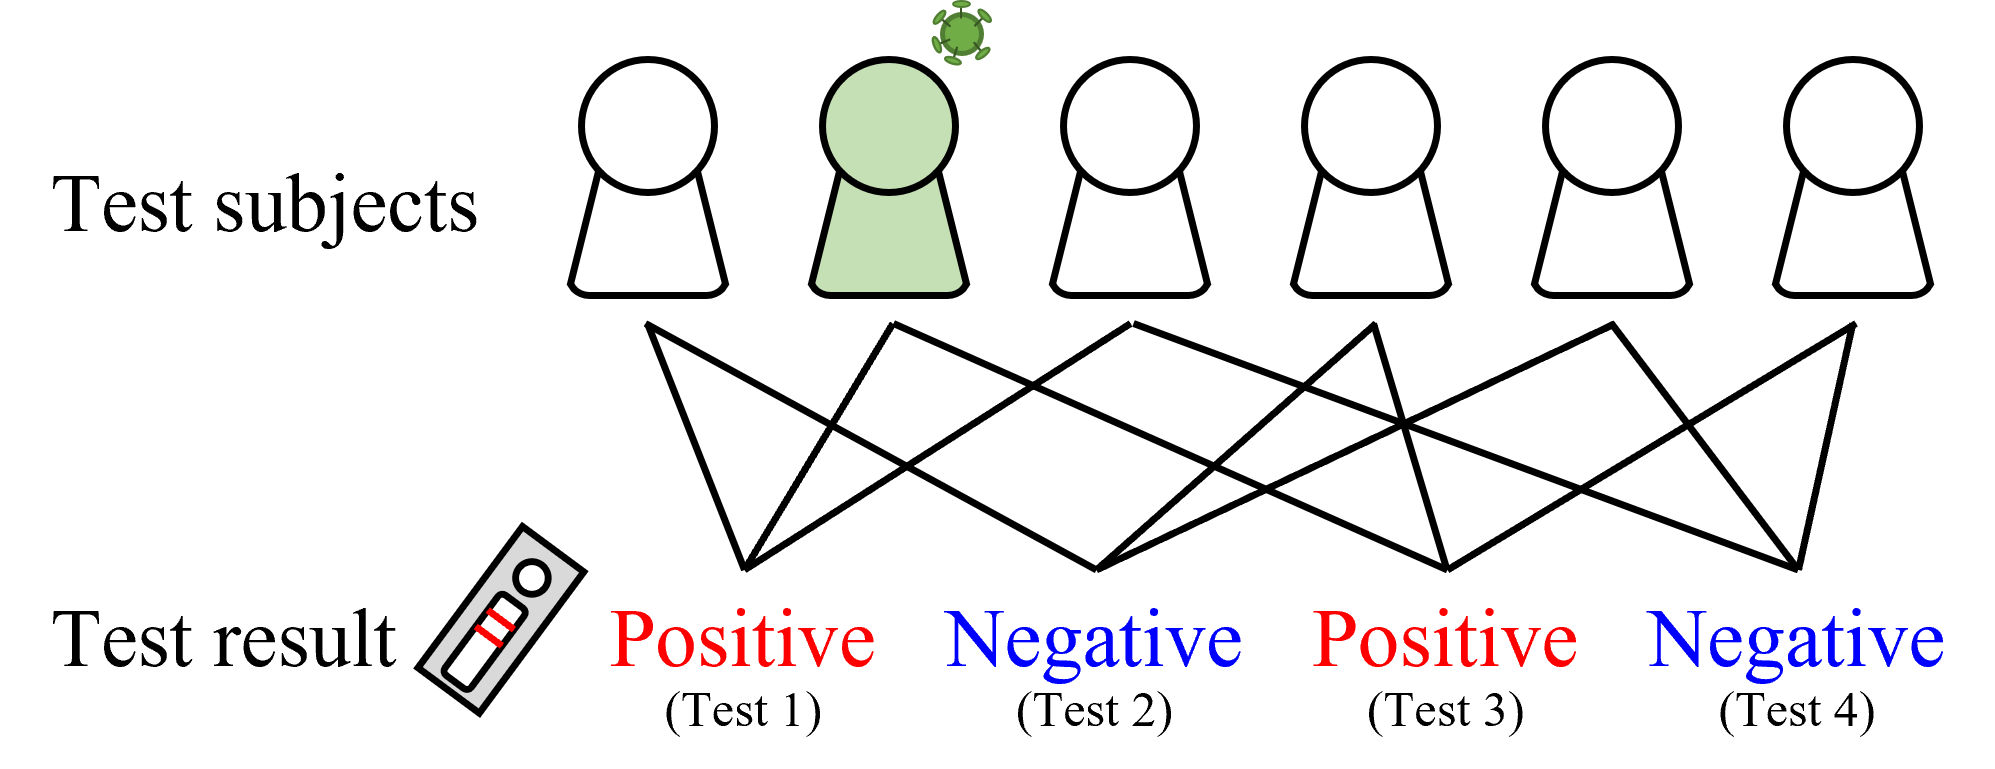
\includegraphics[width=0.6\linewidth]{figures/w11_group_test.png}
    \caption{Group testing. The connected lines show the test subjects sharing a test. The result of a test is negative only if all the people sharing the test is negative (doesn't carry the disease).}
    \label{fig:w11_group_test}
\end{figure}

See the bipartite graph of \autoref{fig:w11_group_test}, we only need $m=4$ tests to determine the infected ones out of $n=6$ people. If a person appears in a negative test, then that person must be negative. The remaining people that cannot be determined are suspicious, and require further testing.

Let us generalize the analysis. Let us use a matrix $A\in\{0,1\}^{m\times n}$ to represent the test schedule, with
\begin{equation}
    A_{ij}:\text{the $i$th test contains the $j$th person.}
\end{equation}
Then we have the result of the $i$th test as
\begin{equation}
    y_i = \bigvee_{j=1}^n (A_{ij} \wedge x_j),
\end{equation}
where $x_j\in\{0,1\}$ is 1 if and only if the $j$th person is infected. The symbol $\vee$ and $\wedge$ represents the logical (boolean) OR and AND operation. As an abuse of notation, one often rewrites the system of equations into the form of $y=Ax$. However, this is by no means a linear algebra problem, it is instead a logic problem.

How do we solve this system of equations to determine $x$?
\begin{example}
    Consider $n=2^5$ and $k=1$, the optimal test is by separating the test subjects into two sets. Consider
    \begin{equation*}
        A = \left[\begin{matrix}
            0 & 0 & 0 & 0 & 0 & 0 & \cdots & 1 \\
            0 & 0 & 0 & 0 & 0 & 0 & \cdots & 1 \\
            0 & 0 & 0 & 0 & 1 & 1 & \cdots & 1 \\
            0 & 0 & 1 & 1 & 0 & 0 & \cdots & 1 \\
            0 & 1 & 0 & 1 & 0 & 1 & \cdots & 1 
        \end{matrix}\right]
    \end{equation*}
    with the $j$th column of $A$ being the binary representation of the number $j$. Then if the $j$th person is infected, i.e. $x_k = \delta_{jk}$, we directly obtain the binary representation of $j$ as $y=Ax$. We only need $m=5$ tests to find the $k=1$ infected person in $n=2^5$ people.
\end{example}

\begin{example}
    \color{red}
    Consider this time $k=2$. For the $j$th column of $A$, let it represent $j$ in its $q$-ary representation ($q=p^n$), for example, $(a_0,a_1,a_2)$. Then we can map $j$ to a polynomial $f(x) = a_0 + a_1x + a_2x^2\in\mathbb{F}_q[x]$. We then evaluate $f$ at $0$, $1$, $\ldots$, $q-1$ and obtain the values $(b_0,b_1,\ldots,b_{q-1})\in\mathbb{F}_q^{q-1}$. We then further turn each $b_i\in\mathbb{F}_q$ into its binary representation, this large vector of 0's and 1's will be the $j$th column of $A$. The decoding then reduces to using the decoding scheme for Reed--Solomon codes.
\end{example}




For more discussions on group testing, please refer to the work by Kautz and Singleton \cite{Kautz_Singleton_64} and \autoref{sec:w12_GT}.
\chapter{Low Density Parity Check Code}
\lecture{22 Apr.}

Coding theory is very much related to the communication protocols we use. In 3G networks, turbo code was used; in 4G, LDPC code was used; and now as of 2025, in 5G, we use a combination of LDPC code and polar code. It would be interesting to see which will appear in our future use of 6G.

Though, as we have seen, polar code is capacity-achieving and it has good second order scaling properties, it is only used in a quarter of the scenarios in 5G; LDPC code, on the other hand, is not capacity-achieving! However, for the block lengths that we cared about, LDPC code is actually better, but it is more of an engineering problem than a theoretical one.

In this chapter, we will dive into the theory and analysis of LDPC code, and see what it has to offer. For more details, one should refer to chapter 3 of ``Modern Coding Theory'' \cite{Modern_Coding_Theory}.

\section{LDPC}
To define a low-density parity-check (LDPC) code, we draw a bipartite graph:

\begin{figure}[H]
    \centering
    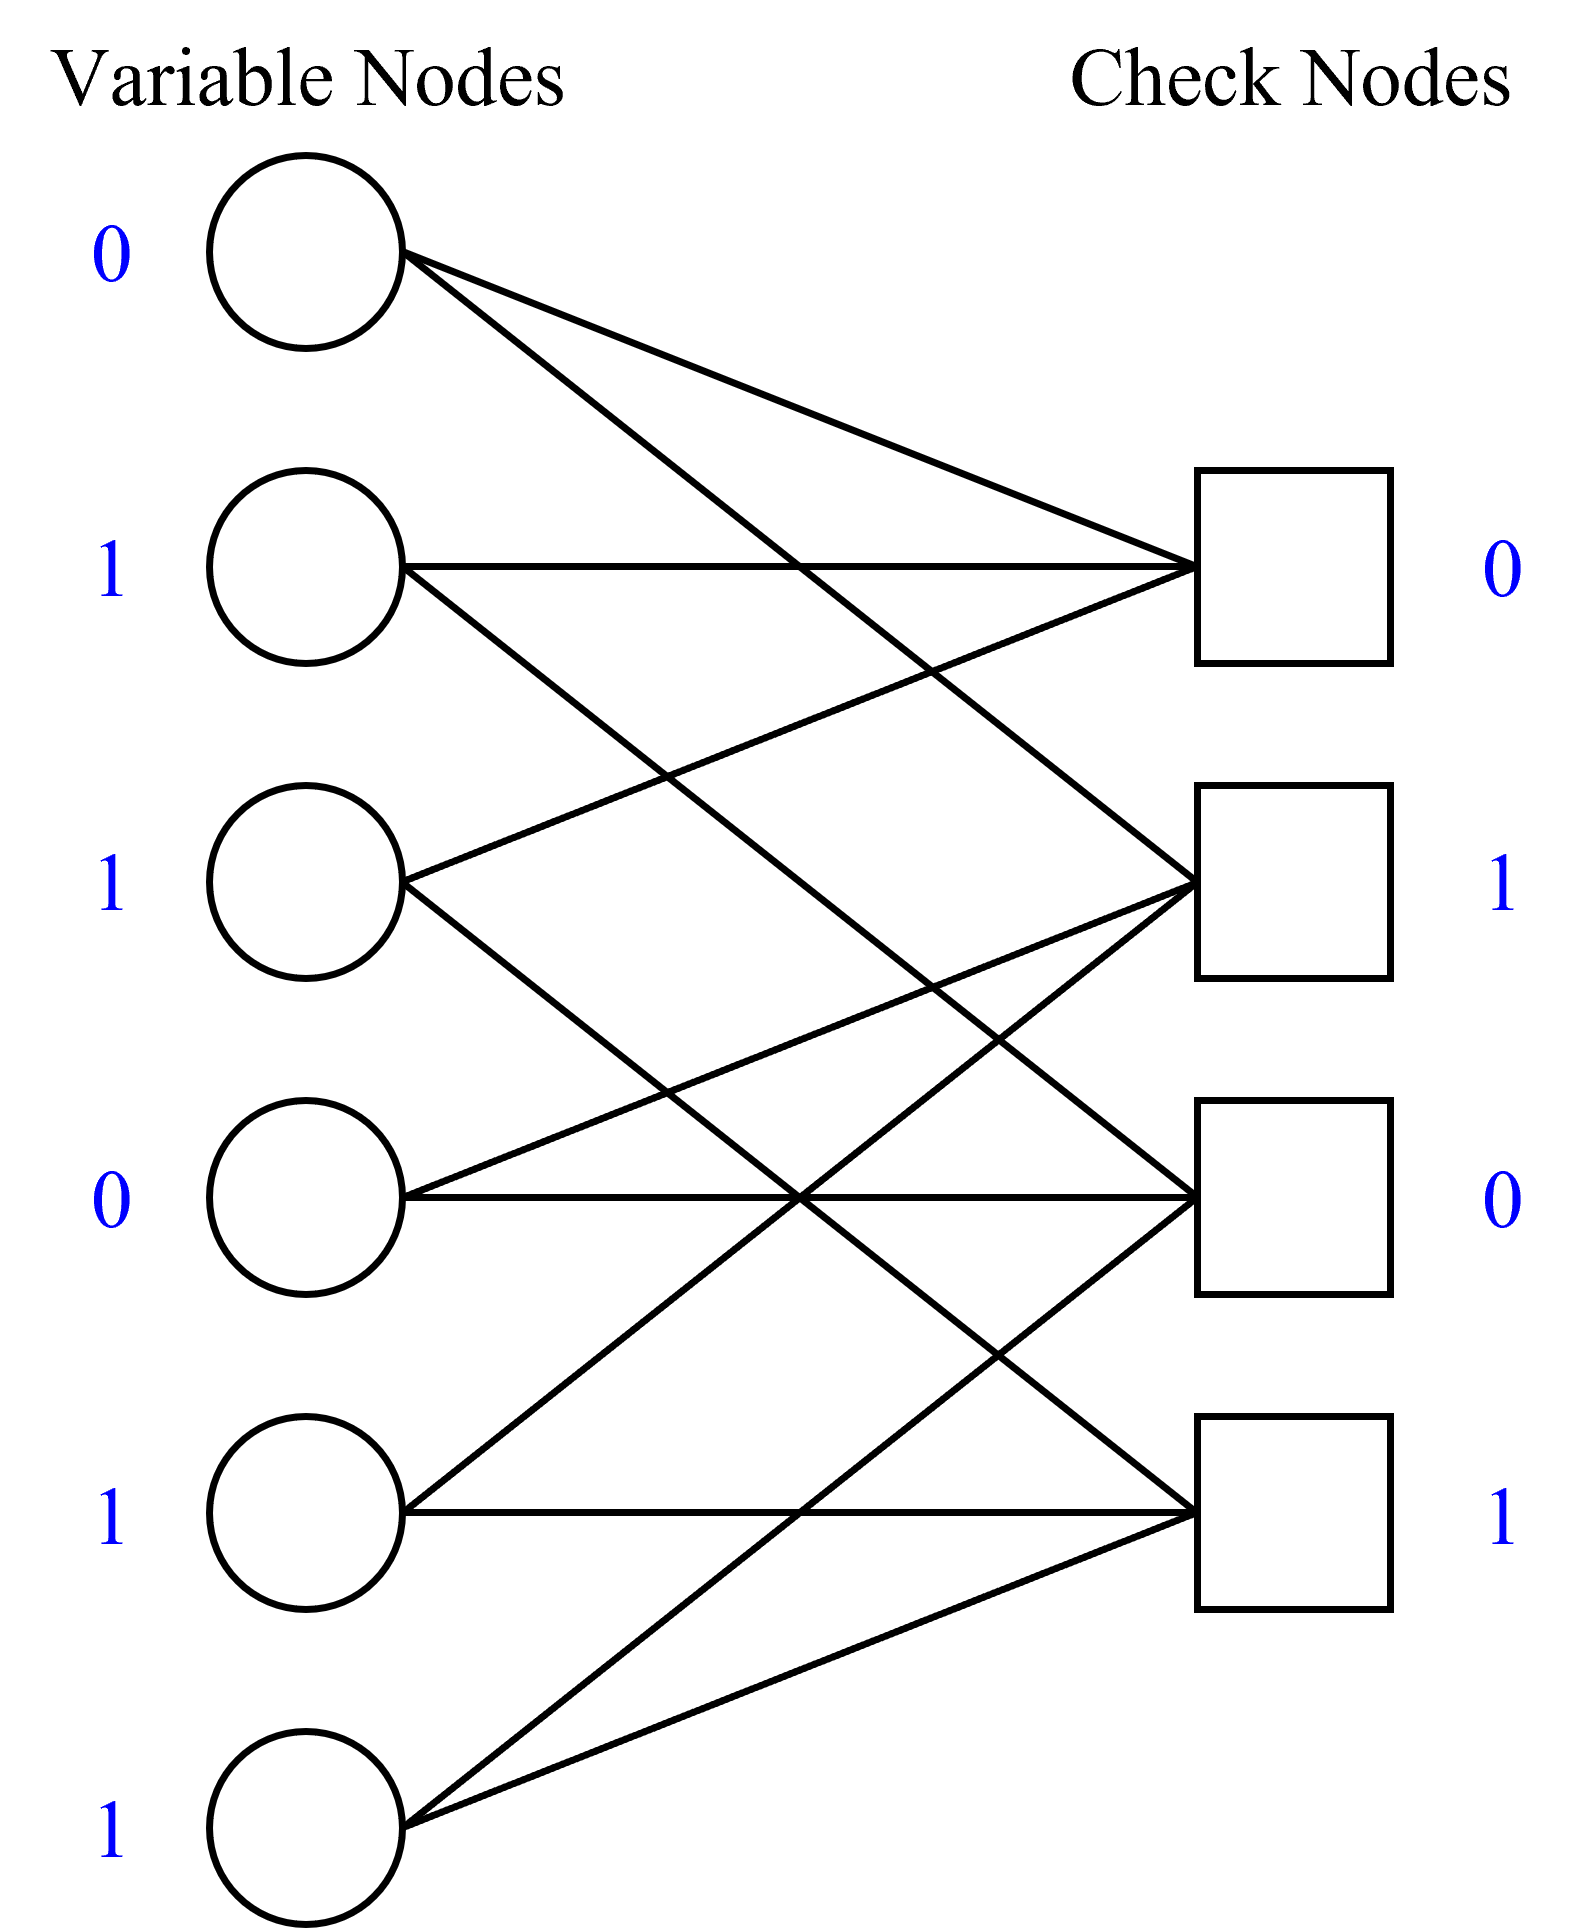
\includegraphics[width=0.4\linewidth]{figures/w10_LDPC.png}
    \caption{Tanner graph of an LDPC code.}
    \label{fig:w10_LDPC}
\end{figure}

The graph consists of two types of nodes: variable nodes (VN) which carry information, and check nodes (CN) who's check sums determine the symptom of a received word. A valid codeword is equal to a vector of assignments on the variable nodes such that all values to the check nodes are zero, else the word is corrupted.

To draw a Tanner graph, it is required that the VN's are drawn on the left, indicated by circular nodes, and the CN's are drawn on the right, indicated by square nodes. Besides \autoref{fig:w10_LDPC}, the only allowed variant of drawing a Tanner graph is \autoref{fig:w10_LDPC_horizontal}.

\begin{figure}[H]
    \centering
    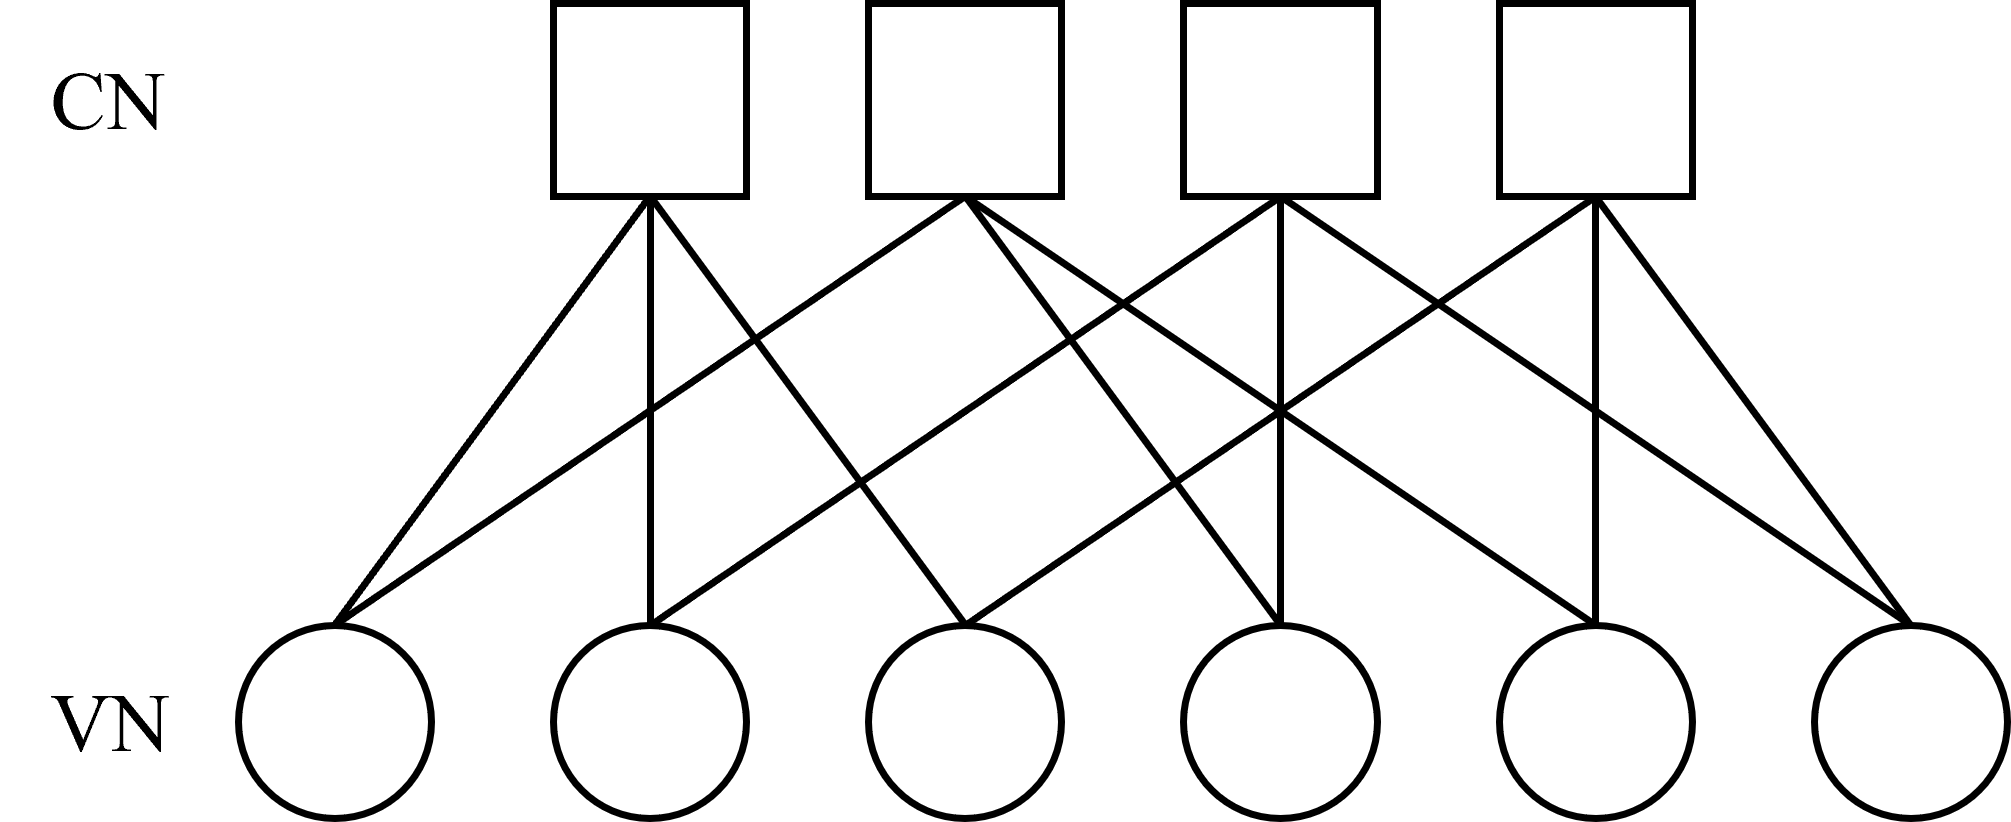
\includegraphics[width=0.5\linewidth]{figures/w10_LDPC_horizontal.png}
    \caption{Horizontal Tanner graph.}
    \label{fig:w10_LDPC_horizontal}
\end{figure}

\begin{definition}[Parity-Check Matrix Formulation]
    An LDPC code can be uniquely defined by the \textit{biadjacency matrix} $H\in\mathbb{F}_2^{\abs{\mathrm{VN}}\times\abs{\mathrm{CN}}}$ of the bipartite graph, where $\mathrm{VN}$ is the set of variable notes, and $\mathrm{CN}$ is the set of check nodes. The graph is also called a \textit{Tanner graph}.

    The biadjacency matrix is related to the \textit{adjacency matrix} of the Tanner graph by
    \begin{equation}
        A = \left[\begin{matrix}
            0 & H \\ H^\transpose & 0
        \end{matrix}\right],
    \end{equation}
    where the first $\abs{\mathrm{VN}}$ rows and columns are the VN's, and the latter $\abs{\mathrm{CN}}$ rows and columns are the CN's.
\end{definition}

\begin{example}
    Take \autoref{fig:w10_LDPC} as an example. Listing the ten vertices in order from VN to CN, from top to bottom, we have the following biadjacency matrix:
    \begin{equation*}
        H = \left[\begin{matrix}
            1 & 1 & 0 & 0 \\
            1 & 0 & 1 & 0 \\
            1 & 0 & 0 & 1 \\
            0 & 1 & 1 & 0 \\
            0 & 1 & 0 & 1 \\
            0 & 0 & 1 & 1 
        \end{matrix}\right].
    \end{equation*}
    Given a word $w\in\mathbb{F}_2^{\abs{\mathrm{VN}}\times 1}$, one can check whether it is a valid codeword by seeing if $Hw$ is the zero vector or not.
\end{example}

\begin{theorem}[Rate of LDPC Code]
    The rate $R$ of an LDPC code satisfies
    \begin{equation}
        R \ge 1- \frac{\abs{\mathrm{CN}}}{\abs{\mathrm{VN}}},
    \end{equation}
    where the equality is met if and only if $H$ is full rank.
\end{theorem}



\section{LDPC over BEC}
Below we see a couple of examples of LDPC over BEC,

\begin{figure}
    \centering
    \subfloat[Single parity-check code.]{
        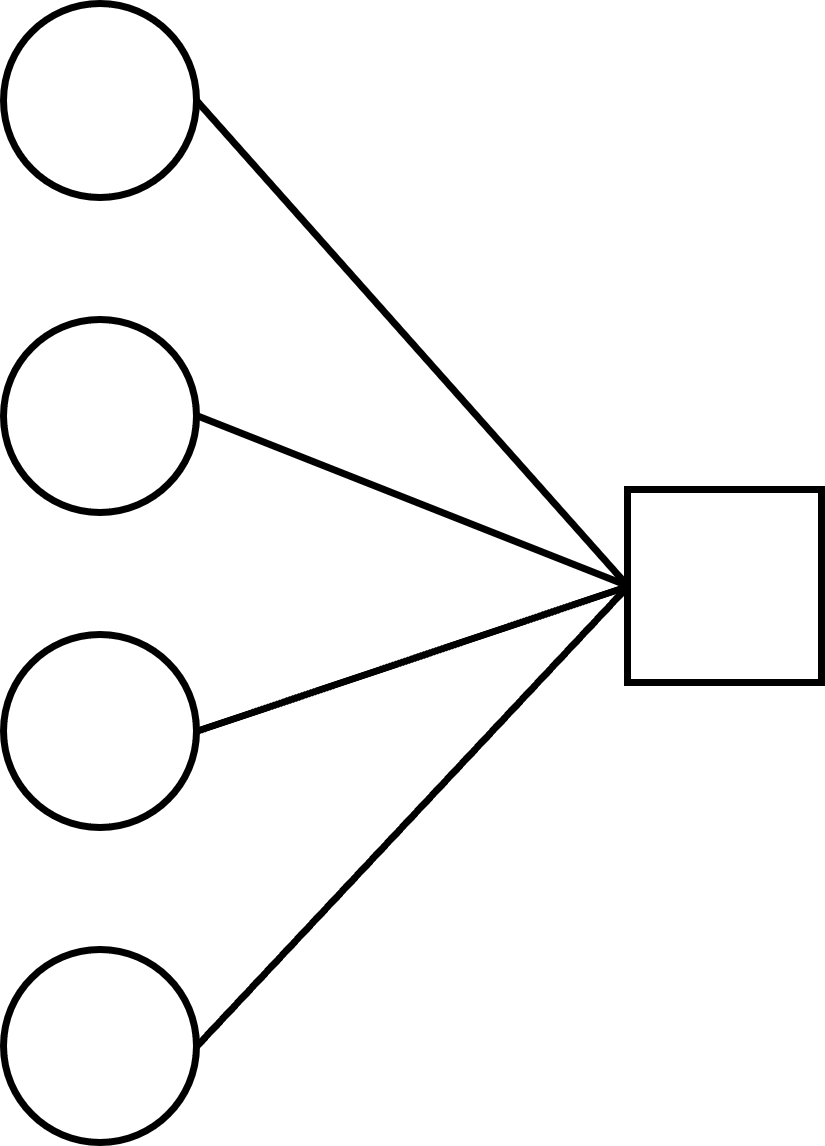
\includegraphics[width=0.25\textwidth]{figures/w10_SPC.png}
        \label{fig:w10_SPC}
    }
    \hspace{1cm}
    \subfloat[Repetition code.]{
        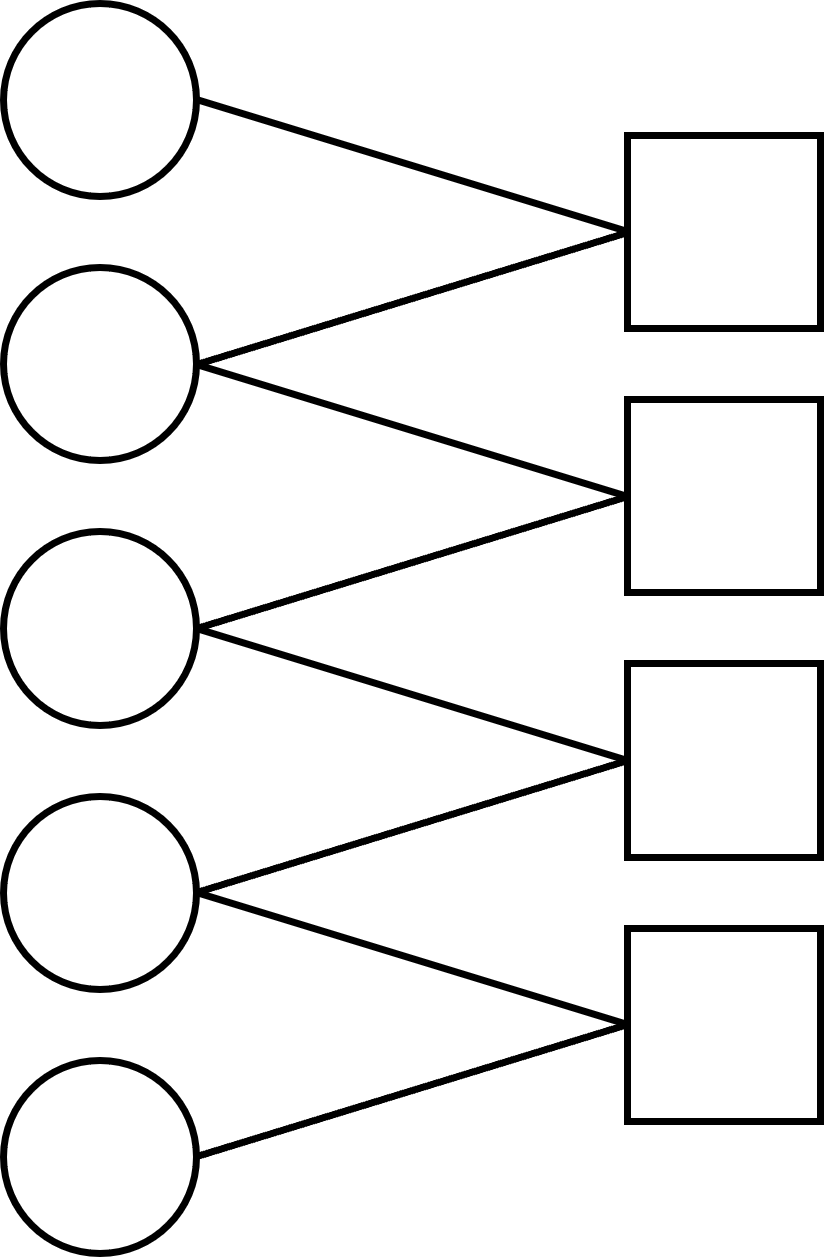
\includegraphics[width=0.25\textwidth]{figures/w10_RC.png}
        \label{fig:w10_RC}
    }
    \hspace{1cm}
    \subfloat[Onion-peeling decoding.]{
        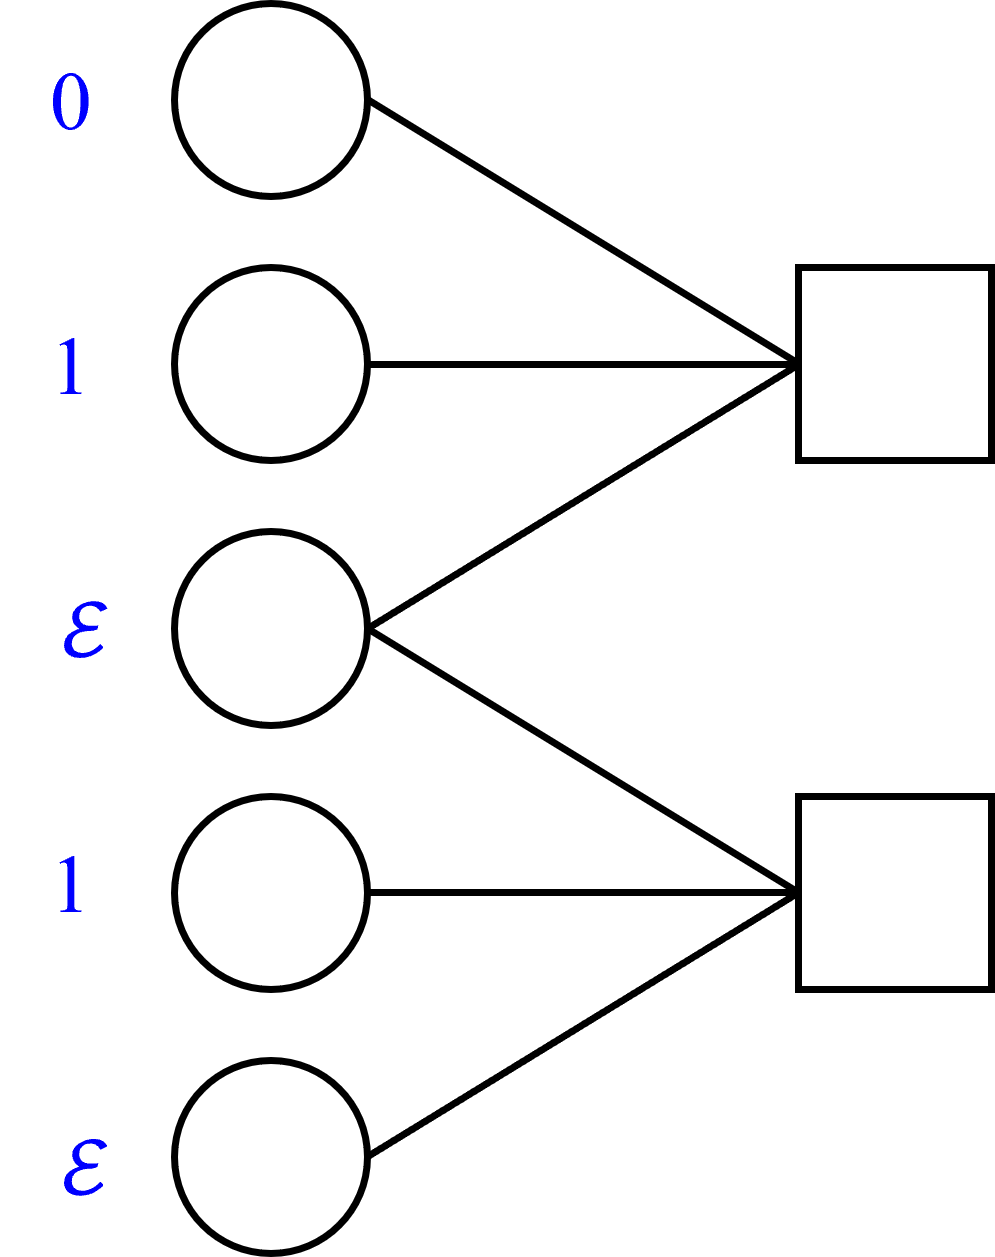
\includegraphics[width=0.28\textwidth]{figures/w10_onion.png}
        \label{fig:w10_onion}
    }
    \caption{LDPC over BEC}
\end{figure}

\begin{example}
    \autoref{fig:w10_SPC} shows the Tanner graph of a single parity-check (SPC) code. The biadjacency matrix of the code is the matrix of ones $H = [1,1,1,1]^\transpose$. If one receives a codeword with a single erasure, say $[0,1,0,\mathcal{E}]^\transpose$, it can be readily seen from the check sum that the erasure should be a 1. However, if there are more than one erasures, say $[0,\mathcal{E},0,\mathcal{E}]^\transpose$, nothing can be learned. Hence, we see that SPC can deal with code having only one erasure.
\end{example}

\begin{example}
    \autoref{fig:w10_RC} shows the Tanner graph of a repetition code (RC). Its biadjacency matrix is a \textit{Toeplitz matrix} of the form
    \begin{equation*}
        H = \left[\begin{matrix}
            1 \\
            1 & 1 \\
            & 1 & 1 \\
            & & 1 & 1 \\
            & & & 1
        \end{matrix}\right],
    \end{equation*}
    and the generator matrix of the codebook is $G=[1,1,1,1,1]$.
\end{example}

\begin{example}
    In \autoref{fig:w10_onion}, we consider decoding with a not-so-trivial LDPC code over a BEC channel. Upon receiving $[0,1,\mathcal{E},0,\mathcal{E}]$, the first CN can immediately recognize that the first erasure is 1. After finding out the first erasure, the second erasure can be determined to be 0 from the second CN.

    This decoding method is called the ``\textit{onion-peeling decoder}.'' Other names exist, too, including the iterative decoder, and my favorite -- the ``sudoku decoder.''
\end{example}

\begin{definition}[Stopping Set / Trapping Set]
    A subset of VN that cannot be decoded if they are all erasure is called a stopping set.
\end{definition}
A stopping set can be removed by adding a new check node, connecting to variable nodes both in the stopping set and outside of the stopping set. However, this decreases the code rate.

\begin{example}
    A common example of stopping sets are cycles. \autoref{fig:w10_cycles} are some examples.
    \begin{figure}[H]
        \centering
        \subfloat[4-cycle.]{
            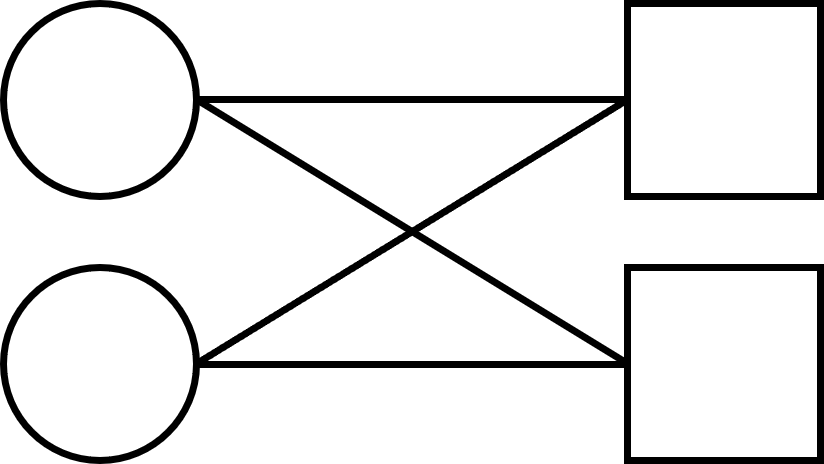
\includegraphics[width=0.2\textwidth]{figures/w10_4cycle.png}
        }
        \hspace{1cm}
        \subfloat[6-cycle.]{
            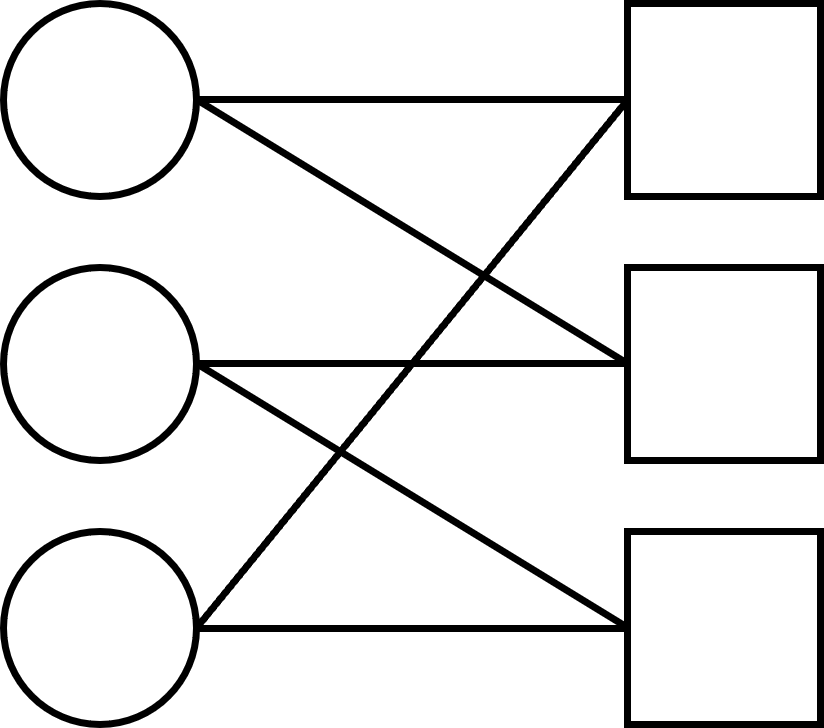
\includegraphics[width=0.2\textwidth]{figures/w10_6cycle.png}
        }
        \caption{Cycles as trapping sets.}
        \label{fig:w10_cycles}
    \end{figure}
    Let the block length of the code be $N$, which is often in the orders of thousands, finding a 4-cycle requires traversing the graph by brute force, requiring a complexity of $O(N^4)$. Similarly, for 6-cycles, $O(N^6)$ computations are needed. The complexity quickly go out of control as the size of the cycle one wish to check increases.
\end{example}


\subsection{Decoding Analysis}
To see whether a setup of VN's and CN's can be decoded, we can analyze the performance on a random graph instead.

\begin{definition}[Regular Graph]
    A graph is regular if $\deg v$ is a constant for all vertex $v$, where $\deg v$ is the amount of edges the vertex is connected to.
\end{definition}

\begin{definition}[Regular LDPC]
    An LDPC code is regular if the degree of the VN's (variable degree) and the degree of the CN's (check degree) are constants.
\end{definition}

\begin{example}
    A $[3,6]$-LDPC is one where its variable degree is 3, and its check degree is 6.
\end{example}

Here we will be dealing with regular LDPC codes, especially having the degree of VN's be 3 and the degree of CN's be 6 such that the rate is $R=1/2$.

Pick a random graph that satisfies the above setup and send a codeword over $\mathrm{BEC}(x)$. Initially, the fraction of VN's that remain as erasures is $x_0\defeq x$.
\begin{figure}[H]
    \centering
    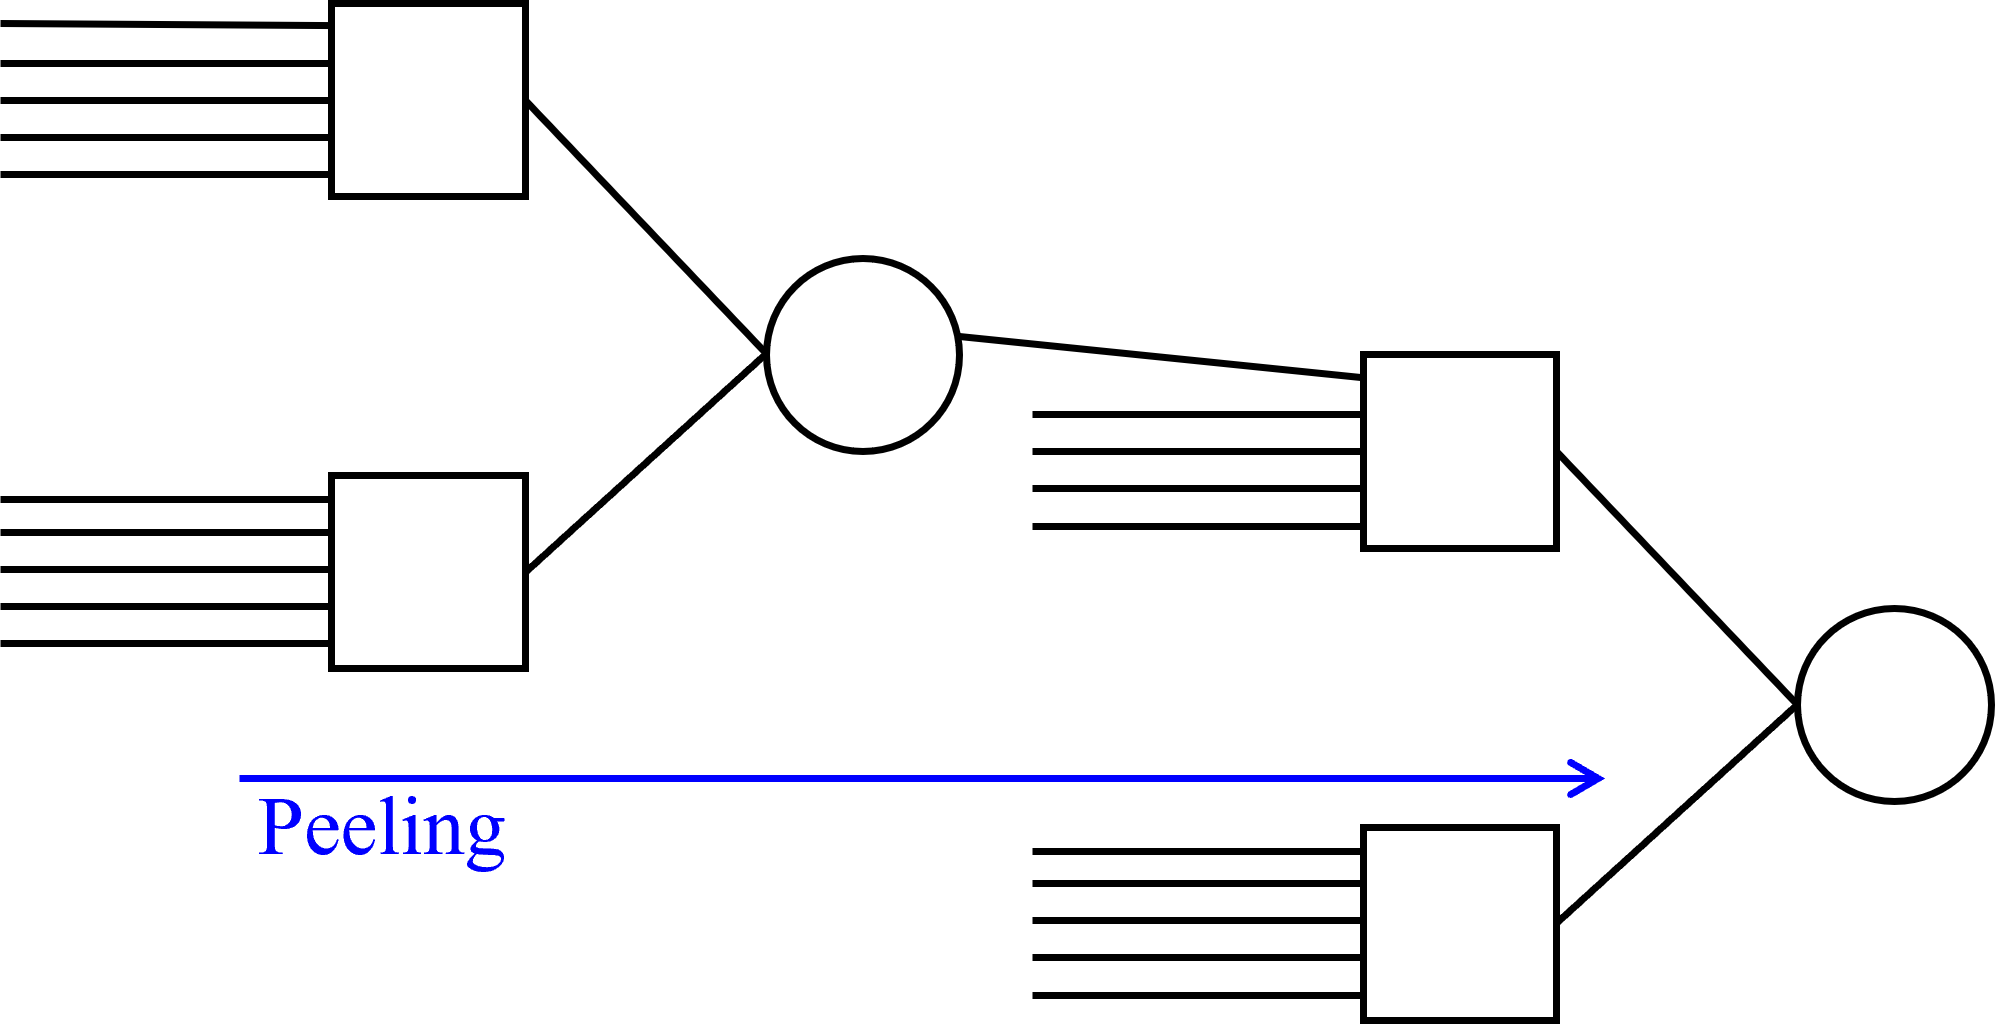
\includegraphics[width=0.5\linewidth]{figures/w10_decoding.png}
    \caption{Tree of onion-peeling / sudoku decoding.}
    \label{fig:w10_decoding}
\end{figure}
After a layer of onion-peeling decoding, a VN that was originally an erasure (say the first VN drawn in \autoref{fig:w10_decoding}) can be decoded if at least one of the check nodes on its left connects to no other erasures. I.e., the remaining fraction of erasures after an iteration becomes
\begin{equation*}
    x_1 \defeq x \left(1-(1-x)^5\right)^2
\end{equation*}
on expectation. If we peel again, the remaining fraction of erasures become
\begin{equation*}
    x_2 \defeq x\left(1-(1-x_1)^5\right)^2.
\end{equation*}
And we do this again and again until achieving $x_n\rightarrow0$, then we ``believe'' that this code is good enough.

Though the iteration is strictly decreasing, it does not always converge to zero. See \autoref{fig:w10_iter_conv} below. Let us consider the code having a rate $R=1/2$, what parameters can the $x_0$ in $\mathrm{BEC}(x_0)$ be so that codewords can be successfully decoded? In theory, the optimal case is $x_0=1/2$. However, by drawing out the iteration
\begin{equation}
    x_n = x_0 \left(1-(1-x_{n-1})^5\right)^2 \label{eq:w10_iteration_example}
\end{equation}
via \autoref{fig:w10_iter_conv_1}, we can see that only when $x_0\lesssim 0.42944$ will the sequence converge to zero. Hence, LDPC code is NOT capacity-achieving.

\begin{figure}[H]
    \centering
    \subfloat[(Part of a) Cobweb plot.]{
        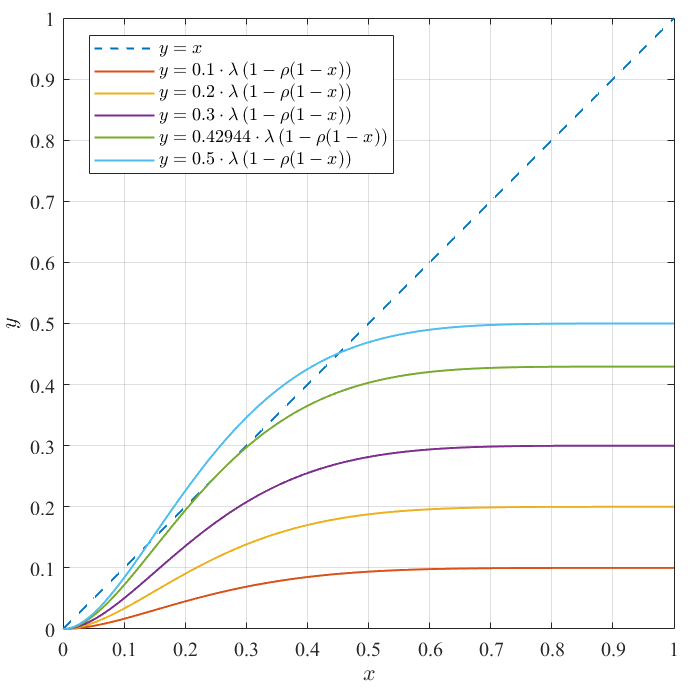
\includegraphics[width=0.475\linewidth]{figures/w10_iter_conv.png}
        \label{fig:w10_iter_conv_1}
    }
    \hspace{0.1cm}
    \subfloat[EXIT chart.]{
        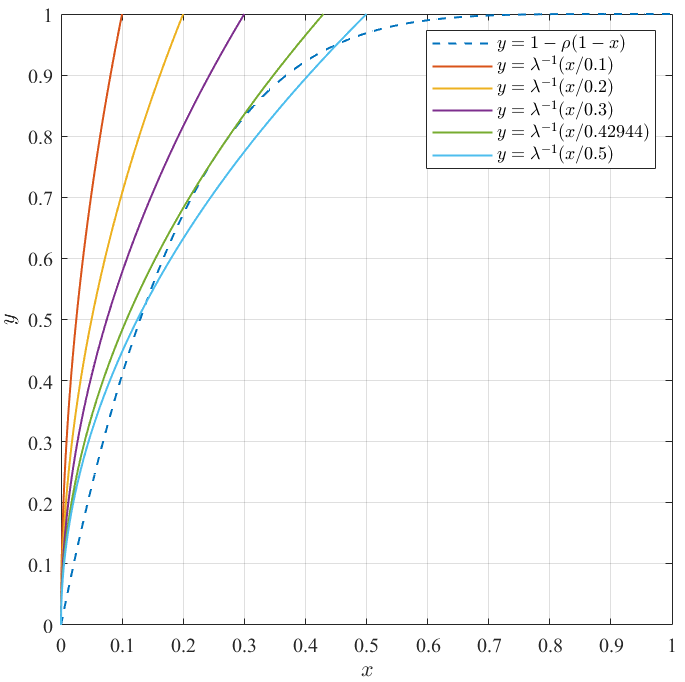
\includegraphics[width=0.475\textwidth]{figures/w10_EXIT_chart.png}
        \label{fig:w10_iter_conv_EXIT}
    }
    \caption{Convergence of fraction of erasures through decoding.}
    \label{fig:w10_iter_conv}
\end{figure}

Another often seen diagram of showing the convergence of the fraction of erasures is the EXIT graph, as seen in \autoref{fig:w10_iter_conv_EXIT}. It performs a transformation on the two curves $y=x$ and $y=x_0(1-(1-x)^5)^2$ to make the analysis for more complicated Tanner graphs simpler, as we will see in the next section.

\section{Irregular LDPC}
In this section we discuss a general LDPC code, containing nodes of various degrees not constrained to be constants, called irregular LDPC.

\begin{definition}[Irregular LDPC]
    For an irregular LDPC, various terms can be defined:
    \begin{itemize}
        \item From the perspective of nodes:
        \begin{align}
            \Lambda_i &\defeq \#\text{ of VN with degree } i, \\
            P_i &\defeq \#\text{ of CN with degree } i,
        \end{align}
        The generating function of the two enumerators are denoted as
        \begin{align}
            \Lambda(x) &\defeq \sum_{i} \Lambda_i x^i, \\
            P(x) &\defeq \sum_{i} P_i x^i.
        \end{align}
        $\Lambda$ and $P$ are the \textit{variable} and $\textit{check degree distributions from a node perspective}$. The normalized degree distributions are
        \begin{align}
            L_i &\defeq \frac{\#\text{ of VN of degree } i}{\#\text{VN}} = \frac{\Lambda_i}{\Lambda(1)}, &L(x) \defeq \sum_{i} L_i x^i = \frac{\Lambda(x)}{\Lambda(1)}, \\
            R_i &\defeq \frac{\#\text{ of CN of degree } i}{\#\text{CN}} = \frac{P_i}{P(1)}, &R(x) \defeq \sum_{i} R_i x^i = \frac{P(x)}{P(1)},
        \end{align}
        the letter $L$ and $R$ stands for left and right, respectively.
        \item From the perspective of edges:
        \begin{align}
            \lambda(x) = \sum_{i} \lambda_i x^{i-1} &\defeq \frac{\Lambda'(x)}{\Lambda'(1)} = \frac{L'(x)}{L'(1)}, \\
            \rho(x) = \sum_{i} \rho x^{i-1} &\defeq \frac{P'(x)}{P'(1)} = \frac{R'(x)}{R'(1)}.
        \end{align}
        The coefficient $\lambda_i\propto i\Lambda_i$ (resp. $\rho_i\propto iP_i$) equals to the fractions of edges that connect to VN's (resp. CN's) of degree $i$. We call $\lambda$ and $\rho$ are the \textit{variable} and \textit{check degree distributions from an edge perspective}.
    \end{itemize}
\end{definition}

\begin{example}
    For a regular LDPC, say the $[3,6]$-LDPC, we have $L(x)=x^3$ and $R(x)=x^6$, with $\lambda(x)=x^2$ and $\rho(x)=x^5$. Note that the iteration \autoref{eq:w10_iteration_example} can be rewritten as
    \begin{equation}
        x_{n} = x_0 \cdot \lambda\left(1-\rho(1-x)\right).
    \end{equation}
    This result can be further generalized.
\end{example}

Consider $L(x) = \frac{1}{2}x^3 + \frac{1}{2}x^4$ and $R(x) = \frac{2}{3}x^6 + \frac{1}{3}x^{20}$. We have $\lambda(x) = \frac{3}{7}x^2 + \frac{4}{7}x^3$ and $\rho(x) = \frac{3}{8}x^5 + \frac{5}{8}x^{19}$. Its Tanner graph can be roughly drawn as in \autoref{fig:w10_irregular_LDPC}, it is a random ensemble of LDPC codes.

\begin{figure}[h]
    \centering
    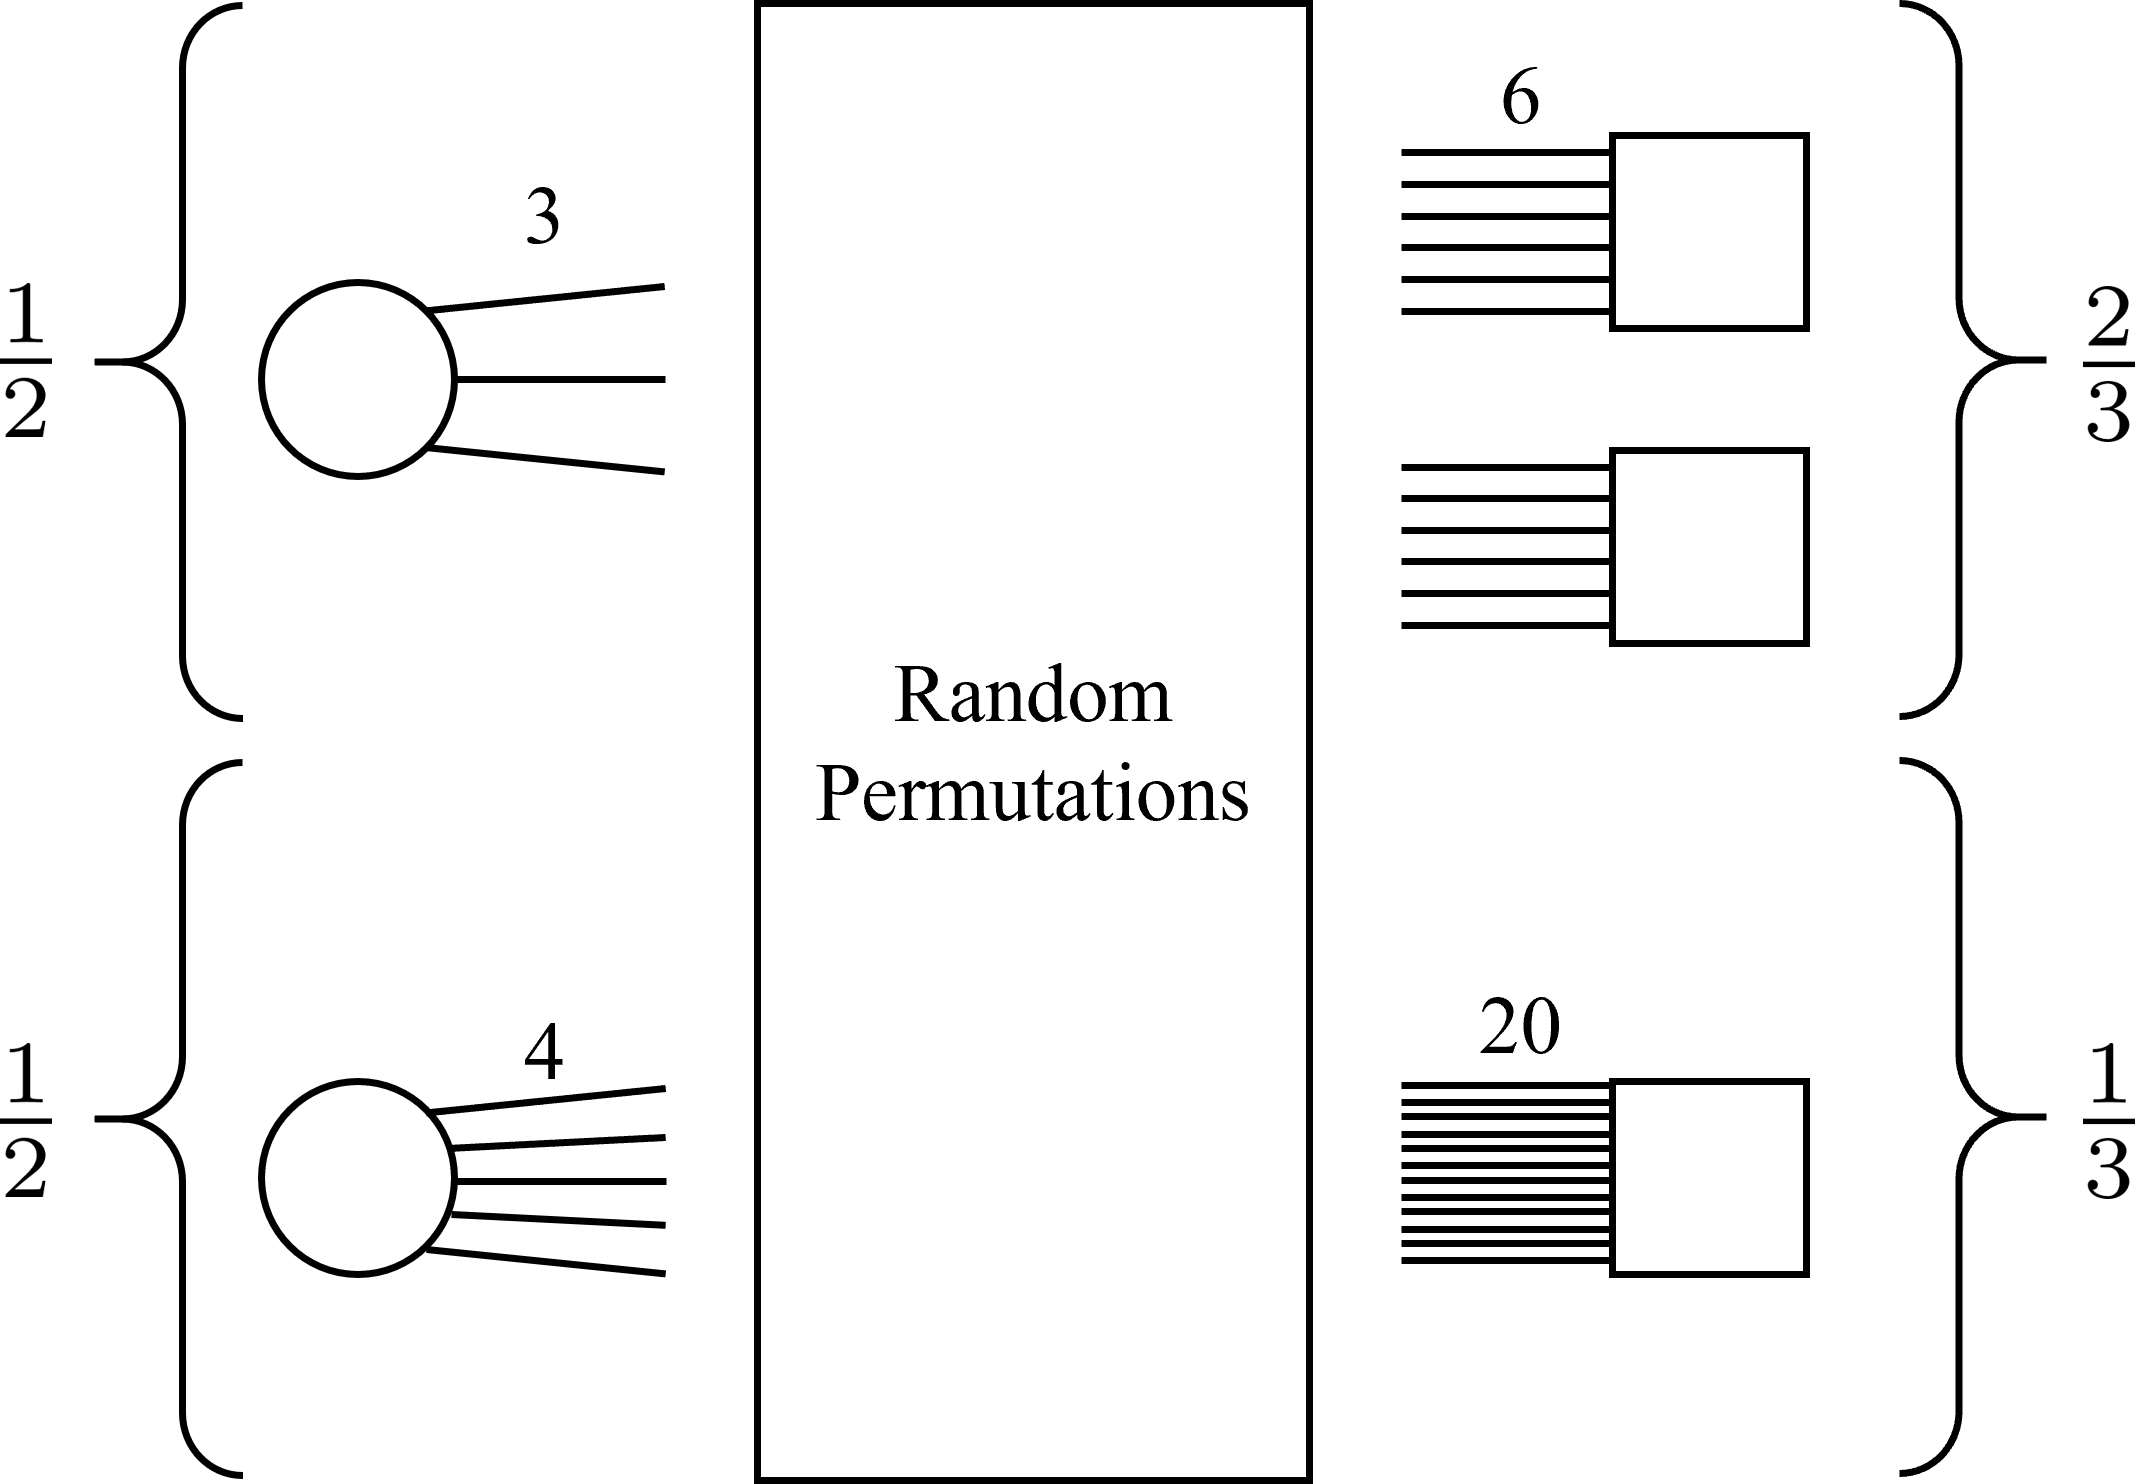
\includegraphics[width=0.5\linewidth]{figures/w10_irregular_LDPC.png}
    \caption{Irregular LDPC with $L(x) = \frac{1}{2}x^3 + \frac{1}{2}x^4$ and $R(x) = \frac{2}{3}x^6 + \frac{1}{3}x^{20}$.}
    \label{fig:w10_irregular_LDPC}
\end{figure}

When applying onion-peeling decoding (refer to \autoref{fig:w10_decoding}), a VN (say $\mathrm{VN}_1$) connects to CN's with 6 edges with probability $\rho_6$, and CN's with 20 edges with probability $\rho_{20}$. Of these CN's with 6 or 20 edges, only 5 or 19 edges are connected to the other VN's. If $\mathrm{VN}_1$ can be decoded successfully, it requires that at least one of the CN's that it is connected to connects to no other erasures. Suppose the fraction of erasures is $x$, the probability on average for a single CN to connect to no erasure is
\begin{equation*}
    \frac{3}{8}(1-x)^5 + \frac{5}{8}(1-x)^{19} = \rho_6(1-x)^5 + \rho_{20}(1-x)^{19} = \rho(1-x).
\end{equation*}
And for each CN, it connects to a degree 3 $\mathrm{VN}_1$ with probability $\lambda_3$, and to a degree 4 $\mathrm{VN}_1$ with probability $\lambda_4$. Since one extra edge of $\mathrm{VN}_1$ should be used to help the future decoding, if $\mathrm{VN}_1$ has degree $i$, we only need one of the remaining $i-1$ check nodes it connected to be helpful. The probability on average that none of the CN's it is connected to is helpful in its decoding will be
\begin{equation*}
    \frac{3}{7}(1-\rho(1-x))^2 + \frac{4}{7}(1-\rho(1-x))^3 = \lambda_3(1-\rho(1-x))^2 + \lambda_4(1-\rho(1-x))^3 = \lambda(1-\rho(1-x)).
\end{equation*}
Henceforth, we see:
\begin{theorem}[Density Evolution] \label{thm:w10_density_evolution}
    The evolution of the density of erasures of an LDPC over $\mathrm{BEC}(x_0)$ after $n$ iterations of decoding follows the following iteration:
    \begin{equation}
        x_{n} = x_0 \cdot \lambda(1-\rho(1-x_{n-1})).
    \end{equation}
\end{theorem}

The iteration between the functions
\begin{align*}
    y_{n} &= x_0\cdot\lambda(1-\rho(1-x_{n-1})),\\
    x_{n} &= y_n
\end{align*}
can be translated the iteration between the functions
\begin{align*}
    y_{n} &= 1 - \rho(1-x_{n-1}), \\
    x_n &= x_0\lambda(y_{n}).
\end{align*}
We can again draw the cobweb plot and EXIT chart as \autoref{fig:w10_iter_conv_2} below. 

The design of a suitable code will hence be translated to the design of suitable polynomials $\rho$ and $\lambda$.

\begin{figure}[H]
    \centering
    \subfloat[Cobweb plot.]{
        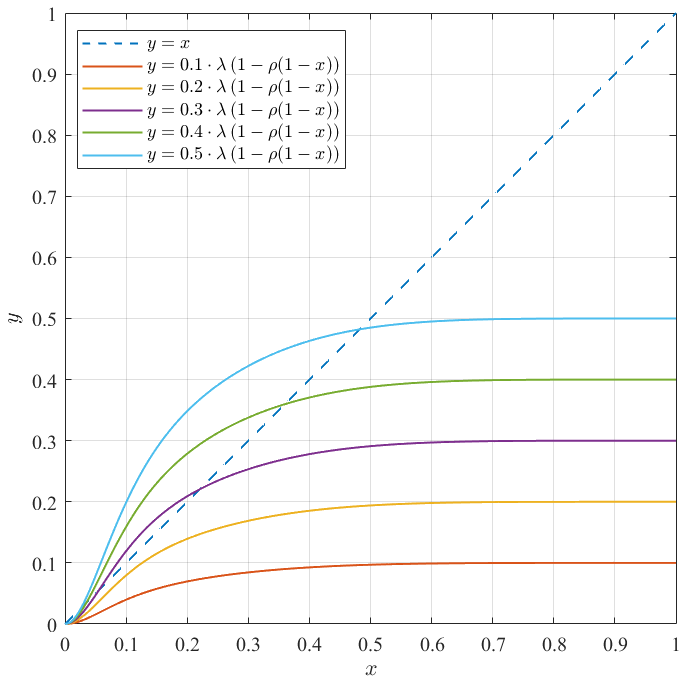
\includegraphics[width=0.475\textwidth]{figures/w10_iter_conv_2.png}
    }
    \hspace{0.1cm}
    \subfloat[EXIT chart.]{
        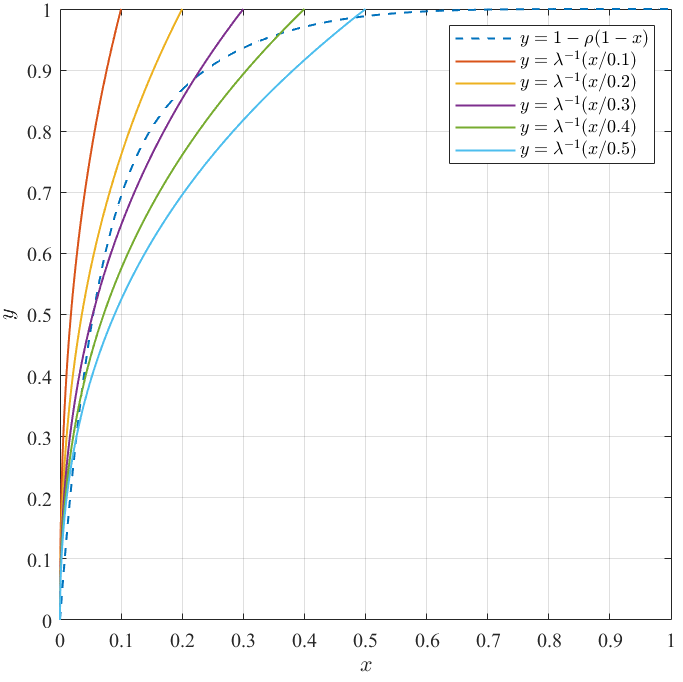
\includegraphics[width=0.475\textwidth]{figures/w10_EXIT_chart_2.png}
    }
    \caption{Convergence of fraction of erasures for $\lambda(x) = \frac{3}{7}x^2 + \frac{4}{7}x^3$ and $\rho(x) = \frac{3}{8}x^5 + \frac{5}{8}x^{19}$.}
    \label{fig:w10_iter_conv_2}
\end{figure}

\section{LDPC over BSC}
\lecture{29. Apr}

Previously, we have studied how to decode an LDPC code over BEC. It is really a simple task, with the erasure density evolving acoording to \autoref{thm:w10_density_evolution}. However, if the decoding is over BSC, this task becomes much more difficult.

Consider the following figure, where we again consider the decoding of a $[3,6]$-LDPC.
\begin{figure}[H]
    \centering
    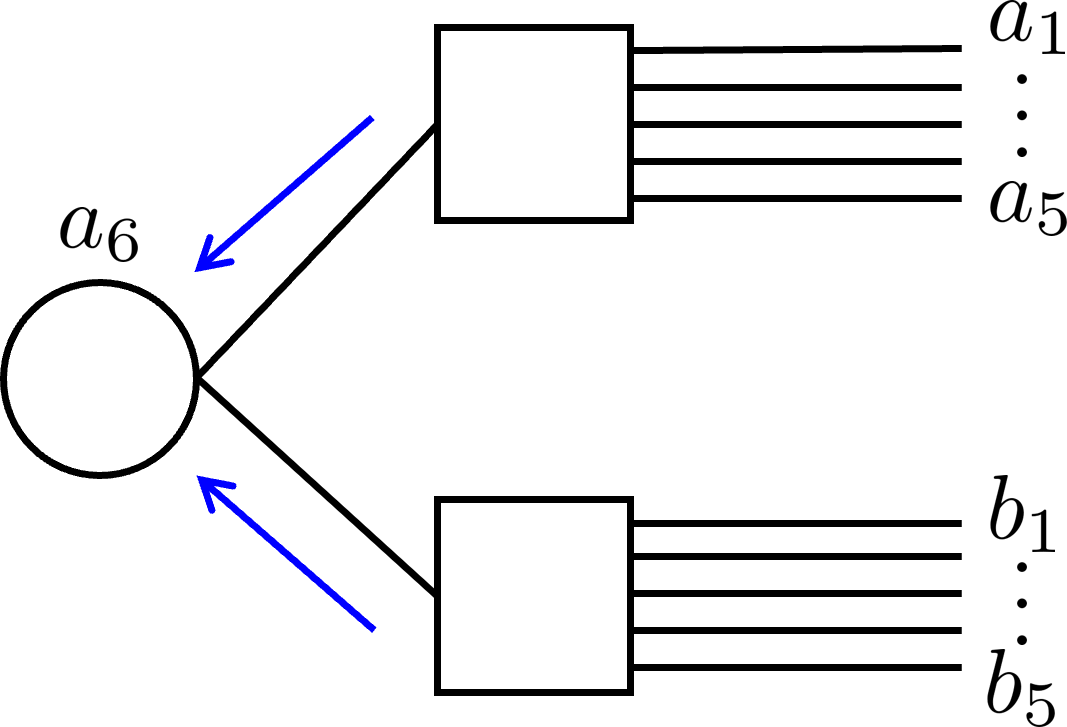
\includegraphics[width=0.3\linewidth]{figures/w11_LDPC_BSC.png}
    \caption{Belief propagation over BSC.}
    \label{fig:w11_belief_prop_BSC}
\end{figure}
If we propagate the value of $a_6$ directly from $a_1$ to $a_5$, then
\begin{equation*}
    a_6 = a_1 + \cdots a_5,
\end{equation*}
where the addition is over $\mathbb{F}_2$. However, there might be conflict with the lower branch of
\begin{equation*}
    a_6 = b_1 + \cdots + b_5.
\end{equation*}
One way to solve this conflict is by majority voting, where a variable node updates its value based on the suggestion that is the majority. However, this doesn't work in our case since both options are equally feasible.

A better method will be to utilize a \textit{soft decoder}.

\subsection{Gallager's Algorithm}
Instead of a strong decoder forcing a node to be an exact value causing major conflicts, we can use a soft decoder that \textit{suggests} the value a variable node should be.

For the following discussion, please also refer to \autoref{sec:w5_polar_dec_par_ser}, especially \autoref{thm:w5_TV_multiply} and \autoref{eq:w5_LLR_add}. Each variable node, for example $\mathrm{VN}_i$ now carries the log-likelihood ratio (LLR) of value
\begin{equation}
    \mathrm{LLR}_i = \ln\frac{\mathrm{Pr}\{\mathrm{VN}_i=0\}}{\mathrm{Pr}\{\mathrm{VN}_i=1\}}.
\end{equation}
The LLR can also be transformed into the signed total variational distance (TV) via
\begin{equation}
    \mathrm{TV}_i = \tanh\left(\frac{\mathrm{LLR}_i}{2}\right).
\end{equation}
When the information are sent from $a_1,a_2,\ldots,a_5$ to $a_6$, the combined information is
\begin{equation}
    \mathrm{TV}_{a_6,a_{1:5}} = \prod_{i=1}^5 \mathrm{TV}_{a_i} = \tanh\left(\frac{\mathrm{LLR}_{a_6,a_{1:5}}}{2}\right). 
\end{equation}
However, information from the branch of $b_1,b_2,\ldots,b_5$ should also be considered. Combining with the original LLR that $a_6$ has, its updated LLR will be
\begin{equation}
    \mathrm{LLR}_{a_6,\text{new}} = \mathrm{LLR}_{a_6,\text{old}} + \mathrm{LLR}_{a_6,a_{1:5}} + \mathrm{LLR}_{a_6,b_{1:5}}.
\end{equation}
The propagation and update of the probability of a VN being 0 or 1 is termed the belief propagation.

However, remember that the use of TV's and LLR's are just a matter of representation, and are only used since they are easy to combine under channel serial and parallel combination, respectively. For the example above, $a_6$ is originally a BSC. But after a single iteration of belief propagation, the $a_6$ channel updates to
\begin{equation}
    a_6 \ostar \left(a_1\boxstar\cdots\boxstar a_5\right) \ostar \left(b_1\boxstar\cdots\boxstar b_5\right).
\end{equation}

For a general LDPC over general channels, we have
\begin{theorem}[Density Evolution]
    Given an LDPC code with degree distributions from an edge perspective $\lambda(x)$ and $\rho(x)$. If the channel one communicates over with is $x_0=\mathcal{E}$, then through decoding, the equivalent channel updates according to
    \begin{equation}
        x_{n+1} = \mathcal{E}\ostar \lambda^{\ostar}\left(\rho^{\,\boxstar}(x_n)\right).
    \end{equation}
    The function $\lambda^{\ostar}$ is a polynomial with multiplication as parallel combination (equiv. to addition in the LLR representation); the function $\rho^{\,\boxstar}$ is a polynomial with multiplication as serial combination (equiv. to multiplication in the TV representation).
\end{theorem}

The step $\rho^{\,\boxstar}(x_n)$ worsens the channel, but the step $\mathcal{E}\ostar\lambda^{\ostar}(\ldots)$ improves the channel. As the iteration goes on, we would like to expect that $x_n\rightarrow \mathrm{BSC}(0)$ (the distribution over LLR goes to $\pm\infty$), then the LDPC code can be decoded as the quality of the bits becomes better and better, and the words converges to the correct codeword. If the distribution over LLR stays around zero, however, then we cannot decode the LDPC code. We can see whether decoding is possible or not given $\lambda$ and $\rho$ by plotting the EXIT chart.

\begin{figure}[H]
    \centering
    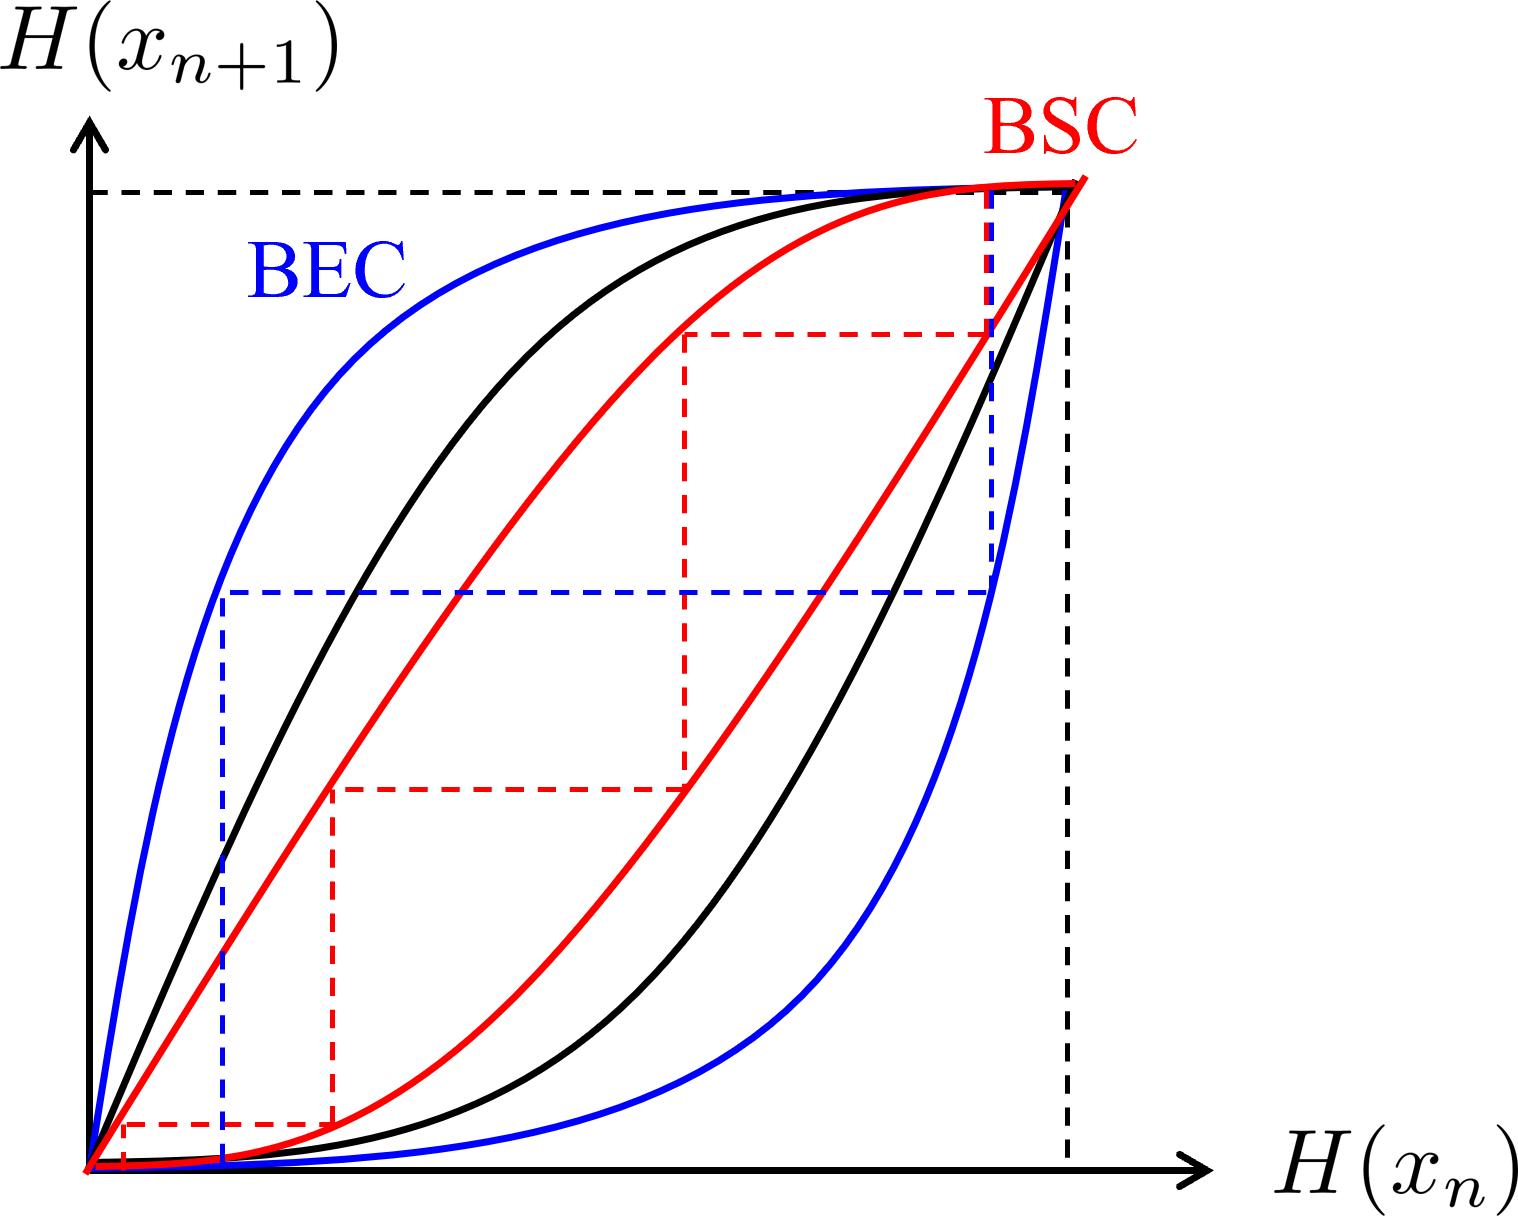
\includegraphics[width=0.5\linewidth]{figures/w11_EXIT.png}
    \caption{Illustration of the EXIT chart of LDPC code over general channels. The blue curves represent BEC, with the best performance; the red curves represent BSC, with the worst performance; the black curves represent any other channel, with intermediate performance.}
    \label{fig:w11_EXIT}
\end{figure}

See \autoref{fig:w11_EXIT}, we use the conditional entropy as an index of the channel quality. The two curves drawn is $(H(x_n),H(y_{n+1})$ and $(H(x_{n+1}),H(y_{n+1}))$, where
\begin{equation}\begin{aligned}
    y_{n+1} &= \rho^{\,\boxstar}(x_n),\\
    x_{n+1} &= \mathcal{E} \ostar \lambda^{\ostar}(y_{n+1}).
\end{aligned}\end{equation}

One can see that BEC converges faster to $(0,0)$ in comparison to BSC, and any other channel has performances in between the former two. Moreover, since the parallel and serial combination of both BEC and BSC remain as BEC and BSC, respectively, we can actually trace the dotted lines on the EXIT chart to see how the entropy evolves as one iterates the decoding scheme. This is not the case for other channels, however. For example, though the parallel combination of AWGN remains AWGN, the serial combination of AWGN becomes a different channel. Hence, one cannot use the EXIT chart to see how the channel conditional entropy iterates.

\begin{remark}
    Even though the serial combination of AWGN is not an AWGN, it is approximately one. Henceforth, as more of an engineering practice, we can assume it to be so and trace the evolution of the mean and variance of the channel output distribution. We can also argue the quality of the channel by seeing how the mean and variance evolve.
\end{remark}
\chapter{Other Topics}
\section{Entropy Complexity}
\lecture{22 Apr.}

This section considers the following task: given $\mathrm{Ber}(1/2)$, how do we generate $\mathrm{Ber}(1/3)$? But before any of that, why is the generation of a random variable so important? If the random numbers generated for security purposes are not ``random'' enough, attackers knowing this knowledge can tailor their attack design to make the encryption scheme especially vulnerable. The generation of a random number is so vital in many of our algorithm design that our societies cannot afford it breaking.

A solution algorithm to the initial problem is shown below:

\begin{figure}[H]
    \centering
    \begin{tikzcd}
	& {\text{ root}} \\
	A && \bullet \\
	& B && {\text{redo}}
	\arrow["{1/2}"', from=1-2, to=2-1]
	\arrow["{1/2}", from=1-2, to=2-3]
	\arrow["{1/2}"', from=2-3, to=3-2]
	\arrow["{1/2}", from=2-3, to=3-4]
    \end{tikzcd}
    \caption{Generating $\mathrm{Ber}(1/3)$ from $\mathrm{Ber}(1/2)$.}
    \label{fig:w10_ber(1/3)}
\end{figure}

See the decision tree above in \autoref{fig:w10_ber(1/3)}. The algorithm starts at the root, and go to either left or right based on the output of a single $\mathrm{Ber}(1/2)$ trial. If ``redo'' is reached, one returns back to the root. The process is repeated until one lands on either $A$ or $B$. The probability of obtaining the two results is
\begin{equation*}
    \mathrm{Pr}\{A\}:\mathrm{Pr}\{B\} = \frac{1}{2}:\frac{1}{4}=2:1 \Rightarrow \mathrm{Pr}\{A\} = \frac{2}{3}, \mathrm{Pr}\{B\}=\frac{1}{3}.
\end{equation*}

This algorithm can be easily generalized. Suppose that we want to generate a random variable following $\mathrm{Pr}\{A\}:\mathrm{Pr}\{B\}:\mathrm{Pr}\{C\} = 1:2:3$, the algorithm can be drawn by a tree of height 3 (since $2^3 > 6 = 1 + 2 + 3$), as shown in the figure below:

\begin{figure}[H]
    \centering
    \begin{tikzcd}
	&&&& {\text{root}} \\
	&& \bullet &&&& \bullet \\
	& \bullet && \bullet & {} & \bullet && \bullet \\
	B & B & A & C && C & C & {\text{redo}} & {\text{redo}}
	\arrow[from=1-5, to=2-3]
	\arrow[from=1-5, to=2-7]
	\arrow[from=2-3, to=3-2]
	\arrow[from=2-3, to=3-4]
	\arrow[from=2-7, to=3-6]
	\arrow[from=2-7, to=3-8]
	\arrow[from=3-2, to=4-1]
	\arrow[from=3-2, to=4-2]
	\arrow[from=3-4, to=4-3]
	\arrow[from=3-4, to=4-4]
	\arrow[from=3-6, to=4-6]
	\arrow[from=3-6, to=4-7]
	\arrow[from=3-8, to=4-8]
	\arrow[from=3-8, to=4-9]
    \end{tikzcd}
    \caption{Generating $\mathrm{Pr}\{A\}:\mathrm{Pr}\{B\}:\mathrm{Pr}\{C\} = 1:2:3$ from $\mathrm{Ber}(1/2)$.}
    \label{fig:w10_tree_1}
\end{figure}

The figure above is a waster of resource, however, and we don't really need to do $\mathrm{Ber}(1/2)$ as many times as it suggests. Of course! We can reduce the tree above to a simpler one below:
\begin{figure}[H]
    \centering
    \begin{tikzcd}
	&&& {\text{root}} \\
	& \bullet &&&& \bullet \\
	B && \bullet & {} & C && {\text{redo}} \\
	& A && C
	\arrow[from=1-4, to=2-2]
	\arrow[from=1-4, to=2-6]
	\arrow[from=2-2, to=3-1]
	\arrow[from=2-2, to=3-3]
	\arrow[from=2-6, to=3-5]
	\arrow[from=2-6, to=3-7]
	\arrow[from=3-3, to=4-2]
	\arrow[from=3-3, to=4-4]
    \end{tikzcd}
    \caption{Reduced tree of \autoref{fig:w10_tree_1}.}
\end{figure}

Let the average number of trials in the above algorithm be $T$, it satisfies
\begin{equation*}
    T = 2\cdot \frac{1}{2} + 3\cdot \frac{1}{4} + 
    T\cdot\frac{1}{4} \Rightarrow T= \frac{7}{3}.
\end{equation*}
This is the optimal algorithm for this example, but in general, how do we know if we can do better? Is there a theoretical bound?

\begin{theorem}[(Knuth \& Yao, 1976) \cite{Complexity_Nonunif_Rand}]
    The amount of bits needed to describe a discrete random variable $X$ is on average at most
    \begin{equation}
        H(X) + 2 \text{ bits}.
    \end{equation}
\end{theorem}
This describes the \textit{entropy complexity} of a random variable. To demonstrate, consider the following example:
\begin{example}
    The worst case possible is if the distribution is the extreme case where the denominator of the distribution is $2^{k}+1$, then we need a tree of $k+1$ layers. Say $\mathrm{Pr}\{A\}:\mathrm{Pr}\{B\} = 2^k:1$, then expected number of $\mathrm{Ber}(1/2)$ trials will be
    \begin{align*}
        x &= \frac{1}{2} + \frac{1}{2^2}(x+1)+\frac{1}{2^3}(x+2)+\cdots+\frac{1}{2^{k+1}}(x+k)+\frac{k+1}{2^{k+1}} \\
        &= \frac{1}{2}\left(1+\frac{k+1}{2^k}\right) + \frac{1}{2}\left(2-\frac{k}{2^k} - \frac{1}{2^{k-1}}\right) + x\left(1-\frac{1}{2^{k}}\right) \\
        \rightarrow x &= \frac{2-(k+2)/2^k}{1-1/2^k}.
    \end{align*}
    The entropy is
    \begin{equation*}
        H(X) = \frac{2^k}{2^k+1}\lg\left(\frac{2^k+1}{2^k}\right) + \frac{1}{2^k+1}\lg(2^k+1).
    \end{equation*}
    We have $x-H(X)$ strictly increasing, and its limit is
    \begin{equation}
        x - H(X) \xrightarrow{k\rightarrow\infty} 2 \text{ bits}. 
    \end{equation}
\end{example}

It seems like $H(X)+2$ is the best guarantee that we can have, and the extra cost of 2 bits is inevitable. Or is it? Given a random vector $Y = (X_1,X_2)$, where $X_1$ and $X_2$ are both i.i.d. copies of $X$. Then, by the theorem above, we will only need
\begin{equation*}
    H(Y) + 2 = 2\left(H(X)+1\right) \text{ bits}.
\end{equation*}
On average, we only need $H(X)+1$ times $\mathrm{Ber}(1/2)$ to generate each $X$. If we want to generate $n$ copies of $X$, then the amount of trials needed becomes $H(X)+\frac{2}{n}$. In the limit, we can achieve the entropy. For example, to simulate rolling a dice, you would need $7+1/3$ times $\mathrm{Ber}(1/2$ trials; however, if you were to simulate two rolls of a dice, you only need to do the Bernoulli trial $13 + 1/3$ times \cite{Complexity_Nonunif_Rand}.

Though we saved the number of Bernoulli trials (the entropy complexity), it tradeoffs with a higher computational complexity.

\begin{remark}
    In the 1976 work by Knuth and Yao \cite{Complexity_Nonunif_Rand}, they discussed the optimality of generating any finite or countably infinite set of rational or irrational probabilities. It is definitely worth a read if one wishes to seek deeper understanding of the topic.
\end{remark}
\section{Group Testing} \label{sec:w12_GT}
\lecture{6 May}

Here we continue on with the discussions on group testing from \autoref{sec:w11_GT}. Let us recap the problem setting: we have $x\in\{0.1\}^{n\times1}$ where $x_i=1$ if and only if the $i$th person is infected, with $m$ being the number of test / measurement. Normally, $k=\norm{x}_0$ is small, for example, $k\sim\sqrt{n}$ or $n^c$ with $c\in[0,1)$, or else the population simply dies out as the disease is so widespread and group testing will be the last of our concerns. Our task is to solve the system of \textit{logical} equations $y=Ax$. One can rewrite this system of logical equations using the usual linear algebra:
\begin{align}
    y^\star &= Ax,\, y^\star_i = \sum_{j}A_{ij}x_j \notag\\
    \Rightarrow y_i &= \min(y^\star_i,1) \\
    \Rightarrow y &= \min(y^\star,\vec{1}),
\end{align}
where $\vec{1}\in\mathbb{R}^{n\times1}$ is the vector of ones.

Besides using the \textit{activation function} $\min(\cdot,1)$, one can opt for arbitrary functions of similar behavior. For example, the ReLU, sigmoid, or $\arctan$ are some suitable replacements. All that is needed is the monotonicity of the activation function. For more information, please refer to the reference \cite{Generalized_Group_Testing}.

\subsection{Applications of Group Testing}
The study of group testing originated during the WWI\!I, where it is used to reduce the amount of test required to find out syphilitic males in soldiers. Nowadays, its applications become almost pervasive, appearing in every corner of modern science. Some examples are listed below, with special emphasis put on heavy hitters and bloom filter.

\paragraph{Genotyping:} The task of genotyping is to find out whether you have a certain strand of gene that, for example, may cause cancer. The human DNA consists of around 3 billion base pairs, it is too costly and impossible to test one-by-one whether a sequence of gene appears in the DNA. Instead, we can use group testing to aid our task. Given a solution of one's DNA, we can apply the CRISPR (a DNA scissor technology) to cut the DNA into suitable strands and heat up the solution so that the double helix unwinds. Next, we prepare a bunch of already-known sequences of cancer genes and connect them with probes that are light emitting when the sequences are bound by its complementary sequence. By mixing the cancer gene sequences with the DNA solution, some of them combines and emits light. Our detector captures this light emission and determines whether a cancer gene is present. Due to the noise inherent in the experiment, this is actually a harder problem of noisy group testing.

\paragraph{Unsourced access:} Given $n$ cellphones near a base station with $k$ of them wanting to talk, how does the base station know which phone is talking what? The time-frequency spectrum is cut into different regions in the communication frequency band: each time slot and frequency slot allows for only one phone transmitting their data (with error correcting code of course). A phone sends its signals by \textit{randomly} choosing a slot. Inevitably, collision may occur where two different phones are talking, and the signals they sent become undecodable. How then, can we resolve collisions in a simplest possible way? The result also requires group testing.

\paragraph{Computer forensics:} Imagine having files saved on your computer and a hacker comes along and modified some of them. How do you detect the modification and fix it, or even better, prevent the modification from even happening? The simplest way is to have your computer never connect to the internet, which is impossible for most practical purposes. Instead, one can utilize what is called a \textit{hash function}. A hash function is a special kind of function that is easy to compute, but \textit{very} difficult to invert, viz., $y=\mathrm{hash}(x)$ is easy to compute, $x=\mathrm{hash}^{-1}(y)$ is hard to compute. For each file, we can create their hash values and store it in a separate database -- so that if a file doesn't match its hash value, we know that it is modified. Except that it doesn't, the hash values can also be modified by the hacker, and a document may be regarded as modified even though it is not! Instead of having a hash value for each file separately, we can group multiple files together to form a single hash value. These hash values are stored in a separate computer. Since the data size for the hash values is smaller then the previous case, we can apply a higher security level on these data to make them difficult to be modified. Just like the bipartite graph of \autoref{fig:w11_group_test}, if a file is modified, some of the hash values do not match, and we can use group testing to pinpoint exactly which file is modified.

\paragraph{Image compression:} An image can be compressed or be represented by fewer bits than its na\"ive representation due to the fact that most natural images are sparse in its Fourier domain. Viz., when applying the Fourier transform to a natural image, most of the Fourier coefficients are close to zero and can be omitted. How do we quickly find out the non-zero coefficients? This task, again, can be solved via group testing. For the more educated readers, one might also draw parallel of this task with the research of \textit{compressed sensing} (or compressive sensing). In fact, they are the same! The only difference lies in their choice of the activation function. For generalized group testing, one might use the logarithmic function as an activation function since it mimics the log-scale sensitivity of human perception (in visual and auditory system).

\paragraph{Heavy hitter:} The task of heavy hitter is to find out which elements are more popular, i.e., which YouTuber has the most subscribers, who's videos has the most view count, which computer file is used most often. Take the last one for example: In a server, we have SSD (solid state drive) and HDD (hard disk drive) as hardware disks, the former is faster in its read and write processing but more expensive, while the latter is slower but cheaper. A reasonable setup is to have, for exmaple, 250GB to SSD used as system disk and 4TB of HDD allocated for saving less-commonly used documents or old photos. Our task is to find out, out of all the $n$ files, which of the $k$ ones are the most popular? It should be noted that the probability of a file being used follows the famous \textit{Zipf distribution}\footnote{This distribution appears everywhere!}, hence only a small fraction of files are actually commonly used, and we can order them from the most often-used ones to the least used ones by allocating them to registers, caches, RAM, SSD, then finally HDD. To efficiently count the frequency of each entry, one can use a \textit{bloom filter}, which will be introduced immediately.

\subsection{Bloom Filter}
When registering for an account on a website, one often sees the sentence ``Invalid username, the username is already taken." How does the server immediately knows that a username appears in the database? It seems impossible to check for every single username in the database for repetition on the fly.

And you are absolutely correct, the server indeed does not check the entire database. Instead, it prepares a string of, for example, 200 bits at hand. The string is all-zero initially when there are no accounts in the database. When an account is added, the database computes a few hash values to the username, these hash values are between 1 to 200. If the username ``apple" is registered, the database computes $\mathrm{hash}(0\text{ apple}) = 10$, $\mathrm{hash}(1\text{ apple}) = 3$, and $\mathrm{hash}(2\text{ apple}) = 5$, then it sets the position 10, 3, and 5 of the bit string to 1. The same applies to all usernames created. Then the final string should consist of 0's and 1's. If one register for a username, the server quickly computes the hash values and compare with its bit string. If all the positions corresponding to the hash values are 1 one the bit string, then it is likely that the username is already taken, and the server rejects your registration (see \autoref{fig:w12_bloom_filter} below). This is the task of membership testing. Although this method has no missed detection, false positives are still possible. That is not a problem, however, since the company is the boss, and it gets to decide which usernames are possible and you can't argue with it. There is one thing this na\"ve bloom filter cannot do, that is, it cannot delete accounts.

\begin{figure}[H]
    \centering
    \begin{equation*}\begin{array}{|c|c|c|c|c|c|c|c|c|c|c|c}
        \hline
        0 & 1 & 1 & 0 & 1 & 0 & 1 & 0 & 0 & 1 & 0 & \cdots \\
        \hline
    \end{array}\end{equation*}
    \caption{Bloom filter. Assume two strings ``apple" and ``banana" added. They have hash values of $10$, $3$, $5$, and $2$, $5$, $7$. If one wants to add ``cherry" into the database, we have to check whether its hash values collide with the 1's in the list.}
    \label{fig:w12_bloom_filter}
\end{figure}

\paragraph{Bloom counter:} Unlike the bloom filter, setting the hash value positions of registered usernames to 1 with logical arithmetic; the bloom counter \textit{adds 1} to the string with usual integer arithmetic. However, now the string will be 200 \textit{bytes} long (1 byte = 8 bits). With this small modification, the bloom counter can delete members. Nevertheless, it cannot delete false positives... why would one implement such functionality anyways?

\begin{figure}[H]
    \centering
    \begin{equation*}\begin{array}{|c|c|c|c|c|c|c|c|c|c|c|c}
        \hline
        0 & 1 & 1 & 0 & 2 & 0 & 1 & 0 & 0 & 1 & 0 & \cdots \\
        \hline
    \end{array}\end{equation*}
    \caption{Bloom counter. Having the same settings as \autoref{fig:w12_bloom_filter}.}
    \label{fig:w12_bloom_counter}
\end{figure}

\paragraph{Database summary:} Given a bloom filter, can we quickly summarize who is in the database? The answer is yes! Though up to a small chance of false positives. The simplest approach is to enumerate all possible accounts and check if they are in the database. If the format of the usernames is restricted, then the set of usernames is finite, and the algorithm converges... after a long time. Instead, we can use a bloom filter to quickly summarize the \textit{heavy hitters} in the database. The technique we will introduce now is called the ``count sketch" or the ``min count sketch", some other algorithms like GroTesQuE (group testing quick and efficient), AC/DC, SAFFRON can also be utilized. We will touch on a few of these methods in a later subsection.

The count sketch method is basically just a bloom counter but with a really nice hash function. Consider having a string of 1000 integers ($\mathbb{Z}^{1000}$), we will now describe the procedure and details of adding an item into the database and summarizing the whole database.
\begin{enumerate}[label=(\arabic*)]
    \item To add ``apple" into the database, turn it into a string of integers, for example, $10010001$. How this string is chosen will be clarified later on.
    \item Find the hash values to ``apple", say we have $\mathrm{hash}(0\text{ apple})=2$ and $\mathrm{hash}(1\text{ apple})=4$.
    \item Add the string $10010001$ to the subarrays with index coinciding with the hash values. See \autoref{fig:w12_database_summary_1}.
    \begin{figure}[H]
        \centering
        \begin{equation*}\begin{array}{|c|c|c|c|c|c}
            \hline
            0\,0\,0\,0\,0\,0\,0\,0 &
            1\,0\,0\,1\,0\,0\,0\,1 &
            0\,0\,0\,0\,0\,0\,0\,0 &
            1\,0\,0\,1\,0\,0\,0\,1 &
            0\,0\,0\,0\,0\,0\,0\,0 &
            \cdots \\
            \hline
        \end{array}\end{equation*}
        \caption{Count sketch: adding an item ``apple" into the database.}
        \label{fig:w12_database_summary_1}
    \end{figure}
    \item Anytime I see ``apple", I add $10010001$ to the above hash-value positions again.
    \item Say we added ``apple" a total of 25 times, and ``banana" a total of 75 times. The string ``banana" is represented by $11001001$, with hash values $4$ and $5$. The fourth subarray should have a value of $100\,75\,0\,25\,75\,0\,0\,100$.
    \item Some other not-so-important entries are added, like ``cherry" 10 times, ``durian" 5 times, and so on. There might also be noise within the data. The final string should have a form similar to \autoref{fig:w12_database_summary_2}.
    \item However, due to the noise present, we cannot immediately find out the heavy hitters. The solution is simple, we can use threholding by, for example, 20.
    \begin{figure}[H]
        \centering
        \begin{align*}
        &\begin{array}{|c|c|c|c|c|c|c}
            \hline
            7\,1\,0\,0\,1\,0\,3\,10 &
            25\,0\,5\,25\,1\,0\,6\,25 &
            0\,3\,0\,3\,1\,0\,0\,10 &
            100\,75\,0\,27\,75\,0\,2\,110 &
            75\,85\,3\,0\,75\,0\,0\,77 &
            \cdots \\
            \hline
        \end{array} \\
        &\downarrow \text{ thresholding by 20} \\
        &\begin{array}{|c|c|c|c|c|c}
            \hline
            0\,0\,0\,0\,0\,0\,0\,0 &
            1\,0\,0\,1\,0\,0\,0\,1 &
            0\,0\,0\,0\,0\,0\,0\,0 &
            1\,1\,0\,1\,1\,0\,0\,1 &
            1\,1\,0\,0\,1\,0\,0\,1 &
            \cdots \\
            \hline
        \end{array}
        \end{align*} 
        \caption{Count sketch: final database followed by thresholding to find the heavy hitters.}
        \label{fig:w12_database_summary_2}
    \end{figure}
    \item The second subarray tells us that ``apple" is a heavy hitter, and the fifth subarray tells us that ``banana" is also a heavy hitter. The fourth subarray, however, is a combination of ``apple" and ``banana", hence it is undecodable. In the case where there is larger noise, we can use error correcting codes (ECC) to set the string representations of ``apple" and ``banana." With ECC used, we can counter with 1 or 2 errors.
\end{enumerate}


\subsection{Binary Search + Group Testing}
The tactics and algorithms for group testing are vast, for further reading, one can refer to the references \cite{CombinatorialGT_SparseRecovery,NoisyNonadaptiveGT,Quickly_Decodable_GT}.

{\color{red}Below, we start our discussion of the na\"ive tactic of binary search. }



\begin{theorem}[Dwass] \label{thm:w12_Dwass}
    The 
\end{theorem}

\begin{remark}
    The original proof to \autoref{thm:w12_Dwass} is given by complex analysis. As a simple excercise, can you think of a combinatorial proof?
\end{remark}
\subsection{Tradeoffs of Group Testing}
\lecture{13 May}

As a final remark to group testing, let us consider the tradeoffs between the five dimensions of group testing:
\begin{enumerate}
    \item Non-adaptive / adaptive: The group testing is done a single round for non-adaptive ones. For adaptive ones it can be done with multiple round, and future rounds can utilize the knowledge gained from past rounds.
    \item The number of tests $m$: we often want $m=O(k\log n)$ since it is the information-theoretic bound. In reality, it might be hard to reach.
    \item Noisy / noiseless: whether you can trust the test results.
    \item Decode complexity: we want it to be $O(k\log n)$, $O(k\,\mathrm{polylog}\,n)$, or $\mathrm{poly}(k\log n)$.
    \item Number of false positives and false negative (\#FP \& FN): should be $O(1)$ or $o(k)$.
\end{enumerate}
Our preferred combination would be to have a nonadaptive noiseless group testing with $O(k\log n)$ tests, $O(k\,\mathrm{polylog}\,n)$ decoding complexity, and 0 FN \& FP with high probability.

The current state of the art can only achieve any combination of four of the above, but never all five.
\begin{enumerate}
    \item If we give up the first:


    \item If we give up the second:


    \item If we give up the third:


    \item If we give up the fourth:


    \item If we give up the fifth:

    
\end{enumerate}

\section{Distributed Matrix Multiplication}

\begin{remark}
    Interestingly enough, just a few days after the lecture, the team of Google Deepmind published a result on fast matrix multiplication from their AI AlphaTensor on 15th of May, 2025. The traditional method of multiplying a $4\times4$ matrix using the Strassen method requires $49$ scalar multiplications. Amazingly, the method proposed by Deepmind requires only $48$ scalar multiplications! What a breakthrough.
\end{remark}
%%%%%%%%%%%%%%%%%%%%%%%%%%%%%%%%%%%%%%%%%%%%%%%%%%%%%%%%

\newpage
\addcontentsline{toc}{chapter}{Bibliography}
\printbibliography
\nocite{*}

\appendix
% \chapter{Weekly Summary} \label{sec:weekly_summary}
% \begin{summary}{1}
    During the first week, the lecturer gave an introduction to how Ar{\i}kan came up with turbo code: as a means to increase the cutoff rate. However, the separation of a channel into sub-channels of inner code is so effective that the outer code can be neglected as a whole. 
    
    An example of given to illustrate the observations is the binary erasure channel. We showed that it is capacity achieving, with capacity of the sub-channels quickly polarize into useful and useless ones.

    The properties of capacity-achieving and polarization is to be discussed in future lectures. One should also pay heeds to the tradeoff between $R$, $p$, and $N$ in coding theory (and their correspondence to deviation theory).
\end{summary}

\begin{summary}{2}
    The Chernoff bound is really useful in showing the achievability of zero error probability in the limit of $n\rightarrow 0$.

    It is truly amazing how the polar code decoder works. Further, the architecture of its structure is also worth noting, especially how the reordering is done in both encoding and decoding stages. The design of the structure is related to how the decoder is defined.
\end{summary}

\begin{summary}{3}
    The sequential decoding of polar code is: first decode, then send back true values via encoder. The bad channels can be set to have frozen bits so as to be sure of their true values.

    The polarization process of polar code over BEC is a martingale.

    The parallel and serial combination of a BSC is linked to the good and bad sub-channels of polar code. Moreover, the result can be generalized to other channels by the fact that all BMSC can be decomposed into convex combination of BSCs.
\end{summary}

\begin{summary}{4}
    This week, we reviewed the maximum inequality from martingale theory. Moreover, generalized versions of the concentration inequality, namely the Azuma's and McDiarmid's inequalities are also introduced.

    Next, we introduced various methods of source coding. The proof for the different methods are all very much similar. One thing to note is that polar code, besides being capacity-achieving for noisy-channel coding, also proven to be very useful in source coding.
\end{summary}

\begin{summary}{5}
    Many new channel parameters are proposed, forming martingales and supermartingales. Many of the inequalities and equalities still requires further study of their details to make sure that they are in fact written correctly.
    
    By switching between the parameters, one can relate with the polar transformation introduced very early on. Interestingly, we also discussed how, in real life, the polar decoder is implemented using log likelihood ratios.

    Lastly, we discussed the topic of distributed source coding, where the Slepian-Wolf algorithm is of huge importance. We left of with the result of its rate region and a brief illustration of the algorithm.
\end{summary}

\begin{summary}{6}
    This week starts off with the algebra of linear code. The duality of codes is also an interesting property worth investigating. The MacWilliams' identity is also stated without a complete proof. I should spend some time investigate how to prove it.

    Next, many results surrounding polar code were given. The first one was regarding the ``eigenvalue problem'' of the polarization speed. Some details to the proof were glossed over, and simulation is required to convince myself of the result.

    Another result that I still cannot really trust is that for polar codes of large kernels, the sequence $\sqrt{Z_n\wedge\varepsilon}$ is a supermartingale. It is truly amazing how we can just ``construct'' martingales. Speaking of construction, the proof of $Z(W_1\ostar W_2)$ and $T(W_1\boxstar W_2)$ from last week also uses constructed random variables, they require further examination.

    Last result is about the source-channel joint coding property of polar codes. I can understand but can't really accept logically the results brought up. Should spend time look up the paper by Honda and Yamamoto.
\end{summary}

\begin{summary}{7}
    The mock test is hard, but it sheds light on many of the previous not-yet-proven results that we have mentioned in the class. These include the proof to MacWilliams' identity and the fact that the dual of Reed-Muller code is still Reed-Muller.
\end{summary}
\chapter{Extra Proofs to Theorems and Lemmas}
\section{MacWilliams' Identity}

The following proofs follows from the paper ``Weight Enumeration and the Geometry of Linear Codes'' \cite{Greene} by C. Greene.

\subsection{Corank-Nullity Generating Function of the Dual Code} \label{app:Whitney}
This is an alternate proof to \autoref{lem:w7_corank_nullity}.

\begin{proof}
    Denote $E=\{1,2,\ldots,n\}$ be the indices and $S$ a subset of $E$. We denote $r(S)$ the rank of the columns $S$ of a generator matrix of a code $\mathcal{C}$, and $r^*(S)$ the rank of the columns $S$ of a generator matrix of the dual code $\mathcal{C}^\perp$.

    A result from \textit{matroid theory} states that
    \begin{equation}
        r^*(S) = \abs{S} + r(E\backslash S) - r(E).
    \end{equation}
    This equation is related to Tutte-Grothedieck invariance, and is in essence, derived from combinatorics arguments. Hence, this proof actually still uses counting. Nevertheless, let us assume that this equation is known and continue on.

    Let us consider the corank-nullity generating function of the dual code:
    \begin{align*}
        W_{\mathcal{C}^\perp}(x,y) &= \sum_{S\subseteq E} x^{r^*(G) - r^*(S)} y^{\abs{S} - r^*(S)} \\
        &= \sum_{S\subseteq E} x^{(n-k) - (\abs{S} + r(E\backslash S) - r(G))} y^{\abs{S} - (\abs{S} + r(E\backslash S) - r(G))} \\
        &= \sum_{S\subseteq E} y^{r(G) - r(E\backslash S)} x^{(n-\abs{S}) - r(E\backslash S)} = W_\mathcal{C}(y,x).
    \end{align*}
    Thus it is shown.
\end{proof}


\subsection{Greene's Lemma} \label{app:Greene}
This is an alternate proof to \autoref{lem:w7_Greene}.

\begin{proof}
    Let $E=\{1,2,\ldots,n\}$ be the indices for a codeword. The support of a codeword $c\in\mathcal{C}$ is defined as
    \begin{equation*}
        \mathrm{supp}(c) \defeq \setdef{i\in E}{c_i=1}.
    \end{equation*}
    The weight enumerator can then be rewritten as
    \begin{equation*}
        A_\mathcal{C}(x,y) = \sum_{S\subseteq E} \#\setdef{c\in\mathcal{C}}{\mathrm{supp}(c)=S} x^{\abs{S}} y^{n-\abs{S}}.
    \end{equation*}
    The RHS of the statement can then be reduced to
    \begin{align*}
        (y-x)^kx^{n-k} W_\mathcal{C}\left(\frac{2x}{y-x},\frac{y-x}{x}\right) &= \sum_{T\subseteq E} 2^{k-r(T)} x^{n-\abs{T}} (y-x)^{\abs{T}} \\
        &= \sum_{T\subseteq E}\sum_{m=0}^{\abs{T}} (-1)^{\abs{T}-m} 2^{k-r(T)} \binom{\abs{T}}{m} x^{n-m} y^m \\
        &= \sum_{T\subseteq E} \sum_{S\subseteq T} (-1)^{\abs{T}-\abs{S}} 2^{k-r(T)} x^{n-\abs{S}}y^{\abs{S}} \\
        &= \sum_{S\subseteq E} \sum_{T\supseteq S} (-1)^{\abs{T}-\abs{S}} 2^{k-r(T)} x^{n-\abs{S}}y^{\abs{S}}.
    \end{align*}
    Next, we replace $S\mapsto S^\mathrm{c}$ and $T\mapsto T^\mathrm{c}$,
    \begin{align*}
        &= \sum_{S^\mathrm{c}\subseteq E} \sum_{T^\mathrm{c}\supseteq S^\mathrm{c}} (-1)^{\abs{T^\mathrm{c}}-\abs{S^\mathrm{c}}} 2^{k-r(T^\mathrm{c})} x^{n-\abs{S^\mathrm{c}}}y^{\abs{S^\mathrm{c}}} \\
        &= \sum_{S\subseteq E} \left(\sum_{T\subseteq S} (-1)^{\abs{S}-\abs{T}} 2^{k-r(T^\mathrm{c})}\right) x^{\abs{S}} y^{n-\abs{S}}.
    \end{align*}
    We need to show that the term in the bracket is equal to $\#\setdef{c\in\mathcal{C}}{\mathrm{supp}(c)=S}$. This can easily be done by introducing the following lemma.
    \begin{lemma}[M{\"o}bius Inversion]
        For set functions $f$ and $g$, we have
        \begin{equation}
            f(S) = \sum_{T\subseteq S} (-1)^{\abs{S}-\abs{T}} g(T) \Leftrightarrow g(S) = \sum_{T\subseteq S} f(T).
        \end{equation}
    \end{lemma}
    \textit{Proof. (M\"obius inversion)}\;
        The lemma is simply proven below:
        \begin{align*}
            \sum_{T\subseteq S} (-1)^{\abs{S}-\abs{T}} \sum_{V\subseteq T} f(V) &= \sum_{V\subseteq S} \sum_{T\supseteq V} (-1)^{\abs{S}-\abs{T}} f(V) \\
            &= \sum_{V\subseteq S} (-1)^{\abs{S}-\abs{V}} f(V) \sum_{m=0}^{\abs{S}-\abs{V}} \binom{\abs{S}-\abs{V}}{m} (-1)^m \\
            &= \begin{dcases}
                \sum_{V\subseteq S} (-1)^{\abs{S}-\abs{V}} f(V) (1-1)^{\abs{S}-\abs{V}} = 0, &S\neq V;\\
                \sum_{V = S} (-1)^{\abs{S}-\abs{V}} f(V) = f(S), &S=V.
            \end{dcases}\;\;\;\;\;\square
        \end{align*}
        
    % \end{proof}
    With the lemma proven, let us continue with the proof of Greene's lemma. Let the set functions be $f(S) = \#\setdef{c\in\mathcal{C}}{\mathrm{supp}(c)=S}$ and $g(S) = 2^{k-r(S^\mathrm{c})}$. Since
    \begin{align*}
        \sum_{T\subseteq S} \#\setdef{c\in\mathcal{C}}{\mathrm{supp}(c)=T} &= \#\setdef{c\in\mathcal{C}}{\mathrm{supp}(c)\subseteq S} = 2^{k-r(S^\mathrm{c})},
    \end{align*}
    where the last equality is obtained since the generator matrix can be written in the full rank form below through column operations:
    \begin{equation*}
        G = \left[\begin{array}{c:c}
            \mathbb{F}_2^{r(S^\mathrm{c})\times\abs{S}} & \mathbb{F}_2^{r(S^\mathrm{c})\times(n-\abs{S})} \vspace{0.1cm} \\ \hdashline 
            \mathbb{F}_2^{r(S)\times\abs{S}} & 0
        \end{array}\right] \in\mathbb{F}_2^{k\times n}.
    \end{equation*}
    The Greene's lemma is finally proven by applying M\"obius inversion.
\end{proof}

\subsection{MacWilliam's Identity}  \label{app:MacWilliams}
This is an alternate proof to \autoref{thm:w6_McWilliams}.
\begin{proof}
    By directing applying the two lemmas above:
    \begin{align*}
        \frac{1}{\abs{\mathcal{C}}}A_{\mathcal{C}}(y-x,y+x) &= \frac{1}{2^k} (2x)^k(y-x)^{n-k} W_\mathcal{C}\left(\frac{y-x}{x},\frac{2x}{y-x}\right) \\
        &= x^k (y-x)^{n-k} W_{\mathcal{C}^\perp}\left(\frac{2x}{y-x},\frac{y-x}{x}\right) \\
        &= A_{\mathcal{C}^\perp}(x,y).
    \end{align*}
\end{proof}


\section{Catalan Number}
\textcolor{red}{The Catalan numbers show up in numerous combinatorial problems. This section gives a brief introduction to the Catalan number, derive its general formula, and derive its generating function. This section fills in the details missing in the proof of }

\end{document}